\documentclass{report}
\usepackage{ngerman}
\usepackage[latin1]{inputenc}
\usepackage{enumerate}
\usepackage{a4wide}
\usepackage{amssymb}
\usepackage{amsmath}
\usepackage{wasysym}
\usepackage{textcomp}
\usepackage{fancyvrb}
\usepackage{alltt}
\usepackage{fleqn}
\usepackage{epsfig}
\usepackage{theorem}
\usepackage{eurosym}
\usepackage{color}
\usepackage{hyperref}

\usepackage[all]{hypcap}
\hypersetup{
	colorlinks = true, 
	linkcolor  = blue,
	citecolor  = red,
        filecolor  = blue,
        urlcolor   = [rgb]{0.5, 0.0, 0.5},
	pdfborder  = {0 0 0} 
}
\usepackage{fancyhdr}
\usepackage{lastpage} 

\renewcommand*{\familydefault}{\sfdefault}

\pagestyle{fancy}

\fancyfoot[C]{--- \thepage/\pageref{LastPage}\ ---}

\fancypagestyle{plain}{%
\fancyhf{}
\fancyfoot[C]{--- \thepage/\pageref{LastPage}\ ---}
\renewcommand{\headrulewidth}{0pt}
}

\renewcommand{\chaptermark}[1]{\markboth{\chaptername \ \thechapter.\ #1}{}}
\renewcommand{\sectionmark}[1]{\markright{\thesection. \ #1}{}}
\fancyhead[R]{\leftmark}
\fancyhead[L]{\rightmark}

\definecolor{amethyst}{rgb}{0.2, 0.4, 0.6}
\definecolor{orange}{rgb}{1, 0.9, 0.0}
\newcommand{\blue}[1]{{\color{blue}#1}}
\newcommand{\red}[1]{{\color{red}#1}}
\newcommand{\yellow}[1]{{\color{yellow}#1}}

\newcommand{\next}{\vspace*{0.1cm}

\noindent}

\newcommand{\exercise}{\vspace*{0.2cm}
\stepcounter{aufgabe}

\noindent
\textbf{Aufgabe \arabic{aufgabe}}: }

\newcommand{\proof}{\vspace*{0.2cm}

\noindent
\textbf{Beweis}: }

\newcommand{\remark}{\vspace*{0.2cm}

\noindent
\textbf{Bemerkung}: }

\newcommand{\solution}{\vspace*{0.2cm}

\noindent
\textbf{L�sung}: }

\newcommand{\example}{\vspace*{0.2cm}

\noindent
\textbf{Beispiel}: \ }

\newcommand{\dx}{\,\textrm{d}}
\newcommand{\bruch}[2]{\frac{\displaystyle#1}{\displaystyle #2}}
\newcommand{\folge}[1]{\bigl(#1\bigr)_{n\in\mathbb{N}}}
\def\pair(#1,#2){\langle #1, #2 \rangle}

\newcommand{\qed}{\hspace*{\fill} $\Box$
\vspace*{0.2cm}

}
\newcommand{\qeds}{\hspace*{\fill} $\Box$}
\newcommand{\eox}{\hspace*{\fill} $\diamond$
\vspace*{0.2cm}

}
\newcommand{\eoxs}{\hspace*{\fill} $\diamond$}

\newcommand{\var}{\mathrm{Var}}
\newcommand{\ds}{\displaystyle}


{\theorembodyfont{\em}
\newtheorem{Definition}{Definition}
\newtheorem{Satz}[Definition]{Satz}
\newtheorem{Lemma}[Definition]{Lemma}
}

\newcounter{aufgabe}

\title{Wahrscheinlichkeits-Rechnung und Statistik \\[0.3cm]
       {\large --- Eine Einf�hrung --- \\ }
       {\large Unterlagen f�r das Sommersemester 2018}
     }
\author{Prof.~Dr.~Karl Stroetmann}
\date{today}

\date{\today\\[1.5cm]
\begin{minipage}[t]{1.0\linewidth}
\noindent
Dieses Skript ist einschlie�lich der \LaTeX-Quellen sowie der in diesem Skript diskutierten
Programme unter
\\[0.2cm]
\hspace*{1.3cm}
\href{https://github.com/karlstroetmann/Statistik}{\texttt{https://github.com/karlstroetmann/Statistik}}
\\[0.2cm]
im Netz verf�gbar.  Das Skript selbst finden Sie in dem Unterverzeichnis
\href{https://github.com/karlstroetmann/Statistik/tree/master/Skript}{Skript}.
Dort ist das Skript in der Datei
\href{https://github.com/karlstroetmann/Lineare-Algebra/blob/master/Statistik/statistik.pdf}{\texttt{statistik.pdf}}
abgespeichert.
Wenn Sie auf Ihrem Rechner \href{http://git-scm.com/download}{\texttt{git}}
installieren und mein Repository mit Hilfe des Befehls
\\[0.2cm]
\hspace*{1.3cm}
\mbox{\texttt{git clone https://github.com/karlstroetmann/Statistik.git}}
\\[0.2cm]
klonen, dann k�nnen Sie durch den Befehl
\\[0.2cm]
\hspace*{1.3cm}
\texttt{git pull}
\\[0.2cm]
die aktuelle Version meines Skriptes aus dem Netz laden.  Falls Sie Fehler in dem Skript finden,
so bin ich f�r Hinweise an die Email-Adresse
\\[0.2cm]
\hspace*{1.3cm}
\href{mailto:karl.stroetmann@dhbw-mannheim.de}{\texttt{karl.stroetmann@dhbw-mannheim.de}}
\\[0.2cm]
dankbar.  Wer sich mit \href{https://en.wikipedia.org/wiki/Git}{git} und
\href{https://www.latex-project.org}{\LaTeX} auskennt, darf mir auch gerne einen 
\href{https://help.github.com/articles/about-pull-requests/}{Pull-Request} schicken.
\end{minipage}
}


\begin{document}

\maketitle
\tableofcontents

\chapter{Einf�hrung}
Die Vorlesung ``\blue{Wahrscheinlichkeits-Theorie und Statistik}'' besch�ftigt sich sowohl mit der
\href{https://de.wikipedia.org/wiki/Wahrscheinlichkeitstheorie}{Wahr\-scheinlichkeits-Theorie}, als auch mit der Anwendung dieser Theorie in der 
\href{https://de.wikipedia.org/wiki/Mathematische_Statistik}{induktiven Statistik}.  Die induktive Statistik
hat im wesentlichen zwei Aufgaben:
\begin{enumerate}
\item Das Sch�tzen von Parameter.

      Nehmen Sie an, Sie m�chten die Lebensdauer einer LED-Lampe herausfinden.  Eine M�glichkeit, diese
      Lebensdauer zu bestimmen, besteht darin, eine Menge verschiedene Lampen solange brennen zu lassen, bis
      sie defekt sind.  Aus der Lebensdauer der einzelnen Lampen versuchen wir dann die
      durchschnittliche Lebensdauer von LED-Lampen abzuleiten.  Hier stellt sich die Frage, wieviele Lampen zu
      testen sind, damit wir eine ausreichende Sicherheit bei der Sch�tzung der Lebensdauer haben.
\item Das Testen von Hypothesen.

      Wird ein neues Medikament entwickelt, so muss unter anderem untersucht werden, ob das Medikament
      einen Beitrag zur Heilung liefert oder ob der Patient ohne das Medikament genauso schnell gesund geworden
      w�re. 
\end{enumerate}
Statistik und Wahrscheinlichkeits-Theorie sind eine der  
Grundlagen des \href{https://en.wikipedia.org/wiki/Machine_learning}{maschinellen Lernens}, das in den letzten
Jahren das Gebiet der \href{https://en.wikipedia.org/wiki/Artificial_intelligence}{k�nstlichen Intelligenz}
revolutioniert hat.  Neben der induktiven Statistik gibt es noch die
\href{https://de.wikipedia.org/wiki/Mathematische_Statistik}{deskriptive Statistik}, deren Aufgabe es ist,
umfangreiche Daten in Kennzahlen zusammenzufassen und diese Daten in Grafiken �bersichtlich anzuordnen.  Aus
Zeitgr�nden werden wir uns mit diesem Teilgebiet der Statistik nur am Rande besch�ftigen k�nnen.

Wir verdeutlichen das grunds�tzliche Vorgehen der induktiven Statistik an einem einfachen Beispiel.
Ein Biologe hat im Wald einen Ameisenhaufen entdeckt und m�chte wissen, wieviele Ameisen
in dieser Kolonie wohnen.  Da es zu aufwendig ist, alle Ameisen zu z�hlen, w�hlt er ein
statistisches Verfahren:  Er f�ngt $1\,000$ Ameisen und markiert diese Ameisen mit einem
Farbtupfer.   Anschlie�end entl�sst er die markierten Ameisen in die Freiheit.
Am n�chsten Tag kommt er wieder und f�ngt  $200$ Ameisen.  Er stellt fest, dass
sich unter diesen Ameisen $5$ Tiere befinden, die einen Farbtuper haben.  Unter der
Annahme, dass sich die Ameisen in der Nacht gut durchmischt haben und dass folglich die
Wahrscheinlichkeit f�r eine Ameise, bei der zweiten Z�hlung gefangen zu werden, unabh�ngig
davon ist, ob die Ameise farblich markiert ist, kann der Biologe nun die Anzahl aller
Ameisen sch�tzen:
\begin{enumerate}
\item Bezeichnet $n$ die Gesamtzahl der Ameisen, so ist der Prozentsatz $p$ der markierten
      Ameisen durch die Formel 
      \begin{equation}
        \label{eq:a0}
        p = \frac{1000}{n}
      \end{equation}
      gegeben.
\item Aus der Voraussetzung, dass die Wahrscheinlichkeit daf�r, dass eine Ameise
      bei der zweiten Z�hlung gefangen wird, unabh�ngig von der Markierung ist,
      folgt, dass f�r die Zahl der gefangenen Tiere, die farblich markiert sind, in 
      etwa 
      \begin{equation}
        \label{eq:a1}
        5 = p \cdot 200
      \end{equation}
      gilt.
\end{enumerate}
Setzen wir den Wert von $p$ aus Gleichung (\ref{eq:a0}) in Gleichung (\ref{eq:a1}) ein, so
finden wir 
\begin{equation}
  \label{eq:a2}
  5 = \frac{1000}{n} \cdot 200 \quad \Leftrightarrow \quad n = \frac{1000 \cdot 200}{5} = 40\,000.
\end{equation}
Der Biologe wird also vermuten, dass die Kolonie von etwa $40\,000$ Ameisen bewohnt wird.
Die hier abgeleitete Formel f�r die Anzahl der Ameisen wird in der Literatur als 
\href{https://en.wikipedia.org/wiki/Mark_and_recapture}{Lincoln-Petersen Sch�tzer}
bezeichnet.

Neben dem Sch�tzwert f�r die Anzahl der Ameisen beantwortet die Statistik zus�tzlich die Frage, wie genau
der angegebene Sch�tzwert ist.  Wir werden im Laufe der Vorlesung ein Verfahren entwickeln, mit
dessen Hilfe wir ein Intervall 
$[n_1,n_2]$ berechnen k�nnen, so dass f�r die Anzahl $n$ der Ameisen die Aussage 
\\[0.1cm]
\hspace*{1.3cm}
$n \in [n_1, n_2]$
\\[0.1cm]
mit einer \blue{Konfidenz} von $95,0\%$ gilt.  Um den Begriff eines solchen
 \href{https://de.wikipedia.org/wiki/Konfidenzintervall}{Kondidenz-Intervalls}
exakt fassen zu k�nnen, m�ssen wir uns zun�chst mit der Wahrscheinlichkeits-Theorie auseinander setzen.


\section{Anwendungen der Theorie der Statistik}
Eine der wichtigsten Anwendungen von Wahrscheinlichkeits-Theorie und Statistik ist das \blue{maschinelle Lernen}, das
im Laufe der letzten Jahre die Grundlage verschiedener spektakul�rer Durchbr�che im Bereich der k�nstlichen
Intelligenz war.  Stellvertretend f�r andere Erfolge m�chte ich hier zuerst das Programm
\href{https://en.wikipedia.org/wiki/AlphaGo}{AlphaGo} nennen, das im Jahre 2017 die Nummer 1 der Weltrangliste
in Go, \href{https://en.wikipedia.org/wiki/Ke_Jie}{Ke Jie} besiegt hat.  Ein anderer Bereich, in dem maschinelles
Lernen einen Durchbruch gebracht hat, ist die Entwicklung
\href{https://en.wikipedia.org/wiki/Autonomous_car}{selbstfahrender Kraftfahrzeuge}, die nach den 
Pl�nen f�hrender Autohersteller im Laufe der n�chsten f�nf Jahre Marktreife erlangen werden.
Neben diesen spektakul�ren Anwendungen der Statistik der letzten Jahre gibt es eine gro�e Zahl von Bereichen,
in denen Statistik schon seit langem eingesetzt wird.  An Stelle einer vollst�ndigen Liste solcher Anwendungen,
die leicht mehrere Seiten f�llen w�rde, m�chte einige wenige Anwendungen herausgreifen, bei denen Statistik
entscheidend ist.
\begin{enumerate}
\item Bei der Messung der Wirksamkeit von \blue{Medikamenten} und \blue{medizinischen Therapien}
      werden seit langem statistische Tests durchgef�hrt.  
      Wird ein neues Medikament eingef�hrt, so reicht es bei der Zulassung nicht aus, jemanden zu kennen, der
      behauptet, dass das Medikament der Tante seines Nachbarn das Leben gerettet hat.  Statt dessen werden
      umfangreiche statistische Tests durchgef�hrt, mit denen die Wirksamkeit eines Medikaments oder einer
      Behandlungsmethode untersucht werden.  Beispielsweise wurde im Jahre 2012 eine umfangreiche statistische
      \href{http://www.telegraph.co.uk/news/health/news/9181445/Breast-cancer-screening-resulting-in-unnecessary-treatment.html}{Studie}
      in Norwegen durchgef�hrt, bei der festgestellt wurde, dass das Brustkrebs-Screening in der bisher
      durchgef�hrten Form sehr fragw�rdig ist und h�ufig zu sinnlosen Behandlungen gef�hrt hat.
\item Im \blue{Versicherungswesen} m�ssen Risiken bewertet werden.  Wahrscheinlichkeits-Theorie und Statistik bilden
      die Grundlage einer solchen Bewertung.
\item Die \blue{Vorhersage eines Wahlausgangs} beruht auf statistischen Erhebungen und
      wahrscheinlichkeits-theoretischen Berechnungen.  Bei der US-amerikanischen Pr�sidentschaftswahl 2016 war
      es entscheidend, das Trump sein Geld genau in den Staaten f�r Werbung eingesetzt hat, die bei der Wahl das Z�nglein
      an der Waage waren.  Bei einer demokratischen Wahl in einem Land wie den USA kommt es entscheidend
      darauf an, wer die besseren Statistiker hat.  Einen interessanten Artikel dazu finden Sie unter
      \\[0.2cm]
      \hspace*{1.3cm}
      \href{https://motherboard.vice.com/en_us/article/mg9vvn/how-our-likes-helped-trump-win}{https://motherboard.vice.com/en\_us/article/mg9vvn/how-our-likes-helped-trump-win}
      \\[0.2cm]
      Das Interessante ist, das Trump bei der Wahl 2016 nur 957,6 Millionen Dollar ausgegeben hat, w�hrend
      Hillary Clinton �ber 1,4 Milliarden Dollar verf�gen konnte, siehe
      \href{https://www.washingtonpost.com/graphics/politics/2016-election/campaign-finance/}{hier}.
      Er konnte die Wahl trotzdem gewinnen, weil sein Team genau ausgerechnet hatte, welche Wahlbezirke mit
      wieviel Geld zu gewinnen waren.  Das erkl�rt auch, warum insgesamt deutlich weniger W�hler f�r Trump
      gestimmt haben als f�r Clinton.  Im US-amerikanischen Wahlsystem kommt es nicht auf die Gesamtzahl
      aller Stimmen an, sondern auf die Gesamtzahl der gewonnenen Wahlbezirke und da lag Donald Trump am Ende
      der Ausz�hlung dann vorne. 
\item In vielen Mannschaft-Sportarten wird heute Statistik eingesetzt, um die Teams optimal zusammen zu
      stellen.  In dem Bestseller \href{https://en.wikipedia.org/wiki/Moneyball}{Moneyball} \cite{lewis:2004}
      beschreibt Michael Lewis, wie es dem Manger \href{https://en.wikipedia.org/wiki/Billy_Beane}{Billy Beane} 
      der \href{https://www.mlb.com/athletics}{Oakland Athletics} Baseball-Mannschaft gelang, das Team aus
      Oakland konkurrenzf�hig zu den \href{https://www.mlb.com/yankees}{New York Yankees} zu machen.  
      Das Buch wurde 2011 verfilmt.
\item Die Anf�nge der Statistik gehen auf Untersuchungen von \blue{Gl�cksspielen} zur�ck.  Da Gl�cksspiele relative
      leicht zu verstehen sind, werden wir uns bei der Einf�hrung der Wahrscheinlichkeits-Theorie bei den
      Anwendungen auf die Untersuchung von Gl�cksspielen beschr�nken.
\end{enumerate}


\section{Literatur}
Es folgt eine subjektive Zusammenstellung von Literatur zur Statistik.  Zus�tzlich zu dem vorliegenden Skript
kann ich Ihnen die folgende Literatur empfehlen.
\begin{enumerate}
\item Das meiner Ansicht nach beste Buch zur Wahrscheinlichkeits-Theorie ist das Buch 
      \blue{Introduction to Probability} von Joseph K.~Blitzstein und Jessica Hwang
      \cite{blitzstein:2014}.  Professor Blitzstein hat die
      \href{https://itunes.apple.com/us/course/statistics-110-probability/id502492375}{Vorlesung}, die diesem
      Buch zu Grunde liegt, auf Video aufgenommen und auf \href{http://stat110.net}{stat110.net} zur Verf�gung 
      gestellt.  
\item Ein weiteres Buch mit dem Titel \blue{Introduction to Probability} stammt von den Autoren
      Charles M.~Grinstead und Laurie J.~Snell \cite{grinstead:97}. Dieses Buch ist ebenfalls sehr
      empfehlenswert und kann unter der  Adresse 
      \\[0.2cm]
      \hspace*{-1.3cm}
      \href{https://www.dartmouth.edu/~chance/teaching_aids/books_articles/probability_book/amsbook.mac.pdf}{
        https://www.dartmouth.edu/\symbol{126}chance/teaching\_aids/books\_articles/probability\_book/amsbook.mac.pdf}
      \\[0.2cm]
      kostenlos aus dem Netz geladen werden.
\item Im Gegensatz zu den beiden vorgenannten B�chern behandelt das Buch \blue{Principles of Statistics} von Michael
      Bulmer \cite{bulmer:1979} sowohl die Wahrscheinlichkeits-Theorie als auch die Anwendung dieser Theorie in der
      Statistik.  Amazon bietet eine preiswerte
      \href{https://www.amazon.de/Principles-Statistics-Dover-Books-Mathematics-ebook/dp/B008TVLLIM/ref=sr_1_1?s=books-intl-de&ie=UTF8&qid=1518381000&sr=1-1&keywords=Bulmer+statistics}{Kindle-Edition}
      f�r \euro\ 9.99 an.
      
\item Das Buch \blue{Statistik --- Der Weg zur Datenanalyse} von Ludwig Fahrmeir und anderen \cite{fahrmeir:2016}
      ist ein gutes
      deutsches Buch zur Statistik.  Es enth�lt allerdings wesentlich mehr Stoff als wir im Rahmen der
      Vorlesung behandeln k�nnen.  Dieses Buch ist in unserer Bibliothek verf�gbar.
\item Als Nachschlagewerk zur Statistik eignet sich das Buch 
      \href{http://www.itl.nist.gov/div898/handbook/index.htm}{Engineering Statistics} \cite{nist:2012}, das vom 
      US-amerikanischen \href{http://www.nist.gov}{National Institute of Standards} herausgegeben wird.
\end{enumerate}



%%% Local Variables: 
%%% mode: latex
%%% TeX-master: "statistik"
%%% ispell-local-dictionary: "deutsch8"
%%% eval: (setenv "LANG" "de_DE.UTF-8")
%%% End: 

\chapter[Wahrscheinlichkeits-Rechnung]{Einf�hrung in die Wahrscheinlichkeits-Rechnung}
Das Leben ist voller Unw�gbarkeiten und Risiken.  Schon die Kelten wussten, dass ihnen jederzeit der Himmel auf
den Kopf fallen konnte.  Gl�cklicherweise passiert so etwas nicht sehr h�ufig.  Trotzdem stellt sich die Frage,
wie \blue{wahrscheinlich} ein solches Ereignis ist.  Zur Beantwortung dieser Frage ist zun�chst der Begriff der
\blue{Wahrscheinlichkeit} festzulegen.  Intuitiv sagen wir, dass ein Ereignis $A$ mit einer Wahrscheinlichkeit
$p$ eintritt, wenn bei $n$-maliger Wiederholung des Experiments das Ereignis $A$ in etwa mit der H�ufikeit
$p \cdot N$ auftritt.  Um der Wahrscheinlichkeits-Begriff genauer festzulegen,  definieren wir den
Begriff des \blue{Zufalls-Experiments}.  Darunter verstehen wir ein Experiment, dessen Ausgang nicht
eindeutig vorbestimmt ist.  Ein Beispiel f�r ein solches Experiment w�re der Wurf einer
M�nze, bei dem als \blue{Ergebnis} entweder \textsl{Wappen} oder \textsl{Zahl} auftritt.  Ein
anderes Zufalls-Experiment w�re der Wurf eines W�rfels, dessen Seiten mit den Zahlen $1$ bis $6$ beschriftet
sind.  Hier k�nnen als Ergebnisse die nat�rlichen Zahlen $1$ bis $6$ auftreten.  Mathematisch werden solche
Zufalls-Experimente durch den Begriff des \blue{Wahrscheinlichkeits-Raums} erfasst.  Wir betrachten zun�chst
den Fall, dass die Menge der Ergebnisse endlich oder abz�hlbar unendlich ist.  In diesem Fall wollen wir von 
einen \blue{diskreten Wahrscheinlichkeits-Raum} sprechen.  Sp�ter werden wir noch den allgemeinen Fall
untersuchen, bei dem die Menge der Ergebnisse �berabz�hlbar ist.  Dieser Fall tritt meistens dann auf, wenn es
sich bei den Ergebnissen des Zufalls-Experiments um reelle Zahlen handelt.


\section{Diskrete Wahrscheinlichkeits-R�ume}
\begin{Definition}[Wahrscheinlichkeits-Raum] \hspace*{\fill} \\
Ein \href{https://de.wikipedia.org/wiki/Wahrscheinlichkeitsraum}{diskreter Wahrscheinlichkeits-Raum}  ist ein Tripel 
 $\langle \Omega, 2^\Omega, P \rangle$, f�r das gilt:
\begin{enumerate}
\item $\Omega$ ist eine Menge, die entweder endlich ist, dann gilt also 
      \\[0.2cm]
      \hspace*{1.3cm} $\Omega = \{ \omega_1, \omega_2, \cdots, \omega_n \}$, 
      \\[0.2cm]
      oder $\Omega$ ist \blue{abz�hlbar unendlich}, dann gilt 
      \\[0.2cm]
      \hspace*{1.3cm}
      $\Omega = \{ \omega_n \mid n \in \mathbb{N} \}$.
      \\[0.2cm]
      Die Elemente von $\Omega$ bezeichnen wir als die \blue{Ergebnisse}
      eines Zufalls-Experiments und die Menge $\Omega$ nennen wir die \blue{Ergebnis-Menge}.
\item $2^\Omega$ ist die Potenzmenge von $\Omega$, also die Menge aller Teilmengen der
      Menge $\Omega$.  Diese Teilmengen bezeichnen wir auch als
      \blue{Ereignisse} und die Menge $2^\Omega$ nennen wir die \blue{Ereignis-Algebra}.
      Mengen der Form $\{\omega_i\}$, die genau ein Element aus $\Omega$ enthalten,
      nennen wir \blue{Elementar-Ereignisse}.
\item $P: 2^\Omega \rightarrow \mathbb{R}$ ist eine Abbildung, die jedem Ereignis 
      $A \subseteq \Omega$ eine reelle Zahl $P(A)$ zuordnet.  Die Zahl $P(A)$ bezeichnen wir als 
      die \blue{Wahrscheinlichkeit}, mit der das Ereignis $A$ eintritt.  
      Die Wahrscheinlichkeit $P$ muss den folgenden \blue{Kolmogorow-Axiomen}
      (\href{https://de.wikipedia.org/wiki/Andrei_Nikolajewitsch_Kolmogorow}{Andrei Nikolajewitsch Kolmogorow};
      1903 -- 1987) gen�gen:
      \begin{enumerate}
      \item $0 \leq P(A) \leq 1$ \quad f�r alle $A \subseteq \Omega$.

            Da wir die Wahrscheinlichkeit $P(A)$ als den Bruchteil aller F�lle, in denen das Ereignis $A$ im
            Durchschnitt eintritt, interpretieren wollen, muss $P(A)$ eine nicht-negative Zahl sein, die
            nicht gr��er als $1$ sein kann.
      \item $P(\emptyset) = 0$.

            Die leere Menge $\emptyset$ bezeichnen wir als das \blue{unm�gliche Ereignis}.
      \item $P(\Omega) = 1$.

            Die Menge $\Omega$ bezeichnen wir als das \blue{sichere Ereignis}.
      \item $A \cap B = \emptyset \rightarrow P(A \cup B) = P(A) + P(B)$ \quad f�r alle $A, B \subseteq \Omega$.

            Schlie�en sich zwei Ereignisse $A$ und $B$ gegenseitig aus,
            gilt also $A \cap B = \emptyset$, so nennen wir diese Ereignisse \blue{unvereinbar}.
            Sind $A$ und $B$ unvereinbare Ereignisse, so ergibt sich die Wahrscheinlichkeit
            des Ereignisses $A\cup B$ als die Summe der Wahrscheinlichkeiten
            der einzelnen Ereignisse.
      \end{enumerate}
      Die Funktion $P$ bezeichnen wir als das \blue{Wahrscheinlichkeits-Ma�}.
\end{enumerate}
\end{Definition}

\noindent
\textbf{Schreibweise}: Das vierte Kolmogorow-Axiom bezeichnen wir als die 
\blue{Additivit�t} des Wahrscheinlichkeits-Ma�es.  Um dieses Axiom einfacher
schreiben zu k�nnen, vereinbaren wir folgende Schreibweise:
 Sind $A$ und $B$ zwei \underline{dis}j\underline{unkte} Mengen, so schreiben wir die
Vereinigung von $A$ und $B$ als $A \uplus B$.  Der Term $A \uplus B$ steht also f�r
zweierlei:
\begin{enumerate}
\item F�r die Vereinigungs-Menge $A \cup B$.
\item F�r die Aussage $A \cap B = \emptyset$.
\end{enumerate}
Mit dieser Schreibweise lautet das Axiom der Additivit�t 
\\[0.2cm]
\hspace*{1.3cm}
$P(A \uplus B) = P(A) + P(B)$.
\\[0.2cm]
Diese Gleichung gilt genau dann, wenn $A \uplus B$ definiert ist und das ist genau dann
der Fall, wenn $A \cap B = \emptyset$ gilt.
\vspace*{0.3cm}

\noindent
\textbf{Beispiel}:  Ein m�glicher Wahrscheinlichkeits-Raum f�r das Zufalls-Experiment 
``W�rfeln mit einem kubischen W�rfel'' ist $\langle \Omega, 2^\Omega, P \rangle$ wobei $\Omega$ und $P$ wie
folgt definiert sind:
\begin{itemize}
\item $\Omega = \{1,2,3,4,5,6\}$,
\item $\ds P(A) = \frac{|A|}{|\Omega|} = \frac{1}{6} \cdot |A|$.

      Hier bezeichnet $|A|$ die Anzahl der Elemente der Menge $A$.  Beachten Sie, dass wir im ersten Semester
      f�r die Anzahl der Elemente die Schreibweise $\textsl{card}(A)$ verwendet haben.  Diese Schreibweise ist
      mir jetzt zu aufwendig.
\end{itemize}
Das Ereignis ``es wurde eine gerade Zahl gew�rfelt'' wird dann durch die Menge
$G = \{2, 4, 6\}$ beschrieben.  F�r die Wahrscheinlichkeit von $G$ gilt 
\\[0.2cm]
\hspace*{1.3cm}
$\ds P(G) = \frac{1}{6} \cdot |G| = \frac{1}{6} \cdot 3 = \frac{1}{2}$.
\\[0.2cm]
Bei dem oben angegebenen Wahrscheinlichkeits-Raum sind wir davon ausgegangen, dass alle
Elementar-Ereignisse dieselbe Wahrscheinlichkeit haben.  Diese Annahme ist  aus
Symmetrie-Gr�nden naheliegend.  In diesem Fall nennen wir das
Wahrscheinlichkeits-Ma� $P$ auch \blue{gleich\-m��ig},  das zugeh�rige
Zufalls-Experiment hei�t dann ein \blue{Laplace-Experiment}
(\href{https://de.wikipedia.org/wiki/Pierre-Simon_Laplace}{Pierre Simon Laplace}; 1749 -- 1827).
Falls die Wahrscheinlichkeit f�r alle Seiten eines W�rfels den selben Wert hat, so
sprechen wir von einem Laplace-W�rfel. \eox

\begin{Definition}[Laplace-Experiment]
Ein Zufalls-Experiment ist ein \blue{Laplace-Experiment} falls der \\
Wahrscheinlichkeits-Raum die Form 
$\langle \Omega, 2^\Omega, P \rangle$ hat, wobei $\Omega$ eine \red{endliche} Menge ist und  und das
Wahrscheinlichkeits-Ma� $P$ f�r eine Ereignis $A \subseteq \Omega$ nach der Formel
\\[0.2cm]
\hspace*{1.3cm}
 $\ds P(A) = \frac{|A|}{|\Omega|}$
\\[0.2cm]
berechnet wird.  Die G�ltigkeit der Kolmogorow-Axiome kann in diesem Fall sofort nachgerechnet werden.
\eoxs
\end{Definition}

\exercise
Es sei $\Omega$ eine endliche Menge.  F�r alle $A \subseteq \Omega$ definieren wir
\\[0.2cm]
\hspace*{1.3cm}
$\ds P(A) := \frac{|A|}{|\Omega|}$.
\\[0.2cm]
Beweisen Sie, dass das Tripel $\langle \Omega, 2^\Omega, P \rangle$ dann ein diskreter Wahrscheinlichkeits-Raum ist.  
\eox


Die Annahme der Gleichm��igkeit des Wahrscheinlichkeits-Ma�es ist logisch nicht
zwingend.  Wenn der W�rfel beispielsweise auf einer Seite mit Blei beschwert ist,
so k�nnte das Wahrscheinlichkeits-Ma� auch wie folgt gegeben sein: 
\\[0.2cm]
\hspace*{1.3cm}
$P\bigl(\{1\}\bigr) = 0.5,\quad P\bigl(\{2\}\bigr) = P\bigl(\{3\}\bigr) = P\bigl(\{4\}\bigr) = P\bigl(\{5\}\bigr) = P\bigl(\{6\}\bigr) = 0.1$.
\\[0.2cm]
Dann w�rden wir f�r das Ereignis ``es wurde eine gerade Zahl gew�rfelt'' gelten: 
\\[0.2cm]
\hspace*{1.3cm}
$P(G) = P\bigl(\{2\}\bigr) + P\bigl(\{4\}\bigr) + P\bigl(\{6\}\bigr) = 0.1 + 0.1 + 0.1 =
0.3$.


\section{Additionss�tze}
Die Kolmogorow-Axiome geben an, wie sich die Wahrscheinlichkeit eines Ereignisses 
$A \cup B$ dann aus den Wahrscheinlichkeiten der Ereignisse $A$ und $B$ berechnen l�sst, wenn die
Ereignisse $A$ und $B$ unvereinbar sind.  Wir wollen jetzt den Fall untersuchen, in dem
$A \cap B \not= \emptyset$ ist, in dem also die Ereignisse $A$ und $B$ gleichzeitig auftreten k�nnen.  In diesem
Fall zerlegen wir die Menge $A \cup B$ in drei 
Teilmengen: 
\\[0.2cm]
\hspace*{1.3cm}
$A \cup B = (A \backslash B) \uplus (B \backslash A) \uplus (A \cap B)$
\\[0.2cm]
Da die drei Mengen $A \backslash B$, $B \backslash A$ und $A \cap B$ paarweise
disjunkt sind, gilt 
\begin{equation}
  \label{eq:u1}
  P(A \cup B) = P(A \backslash B) + P(B \backslash A) + P(A \cap B)
\end{equation}
Au�erdem gilt 
\\[0.2cm]
\hspace*{1.3cm}
$A = (A \backslash B) \uplus (A \cap B)$ \quad und \quad
$B = (B \backslash A) \uplus (A \cap B)$.
\\[0.2cm]
Daraus folgt sofort 
\\[0.2cm]
\hspace*{1.3cm}
$P(A) = P(A \backslash B) + P(A \cap B)$ \qquad und \qquad
$P(B) = P(B \backslash A) + P(A \cap B)$.
\\[0.2cm]
Subtrahieren wir auf beiden Seiten dieser Gleichungen den Term $P(A \cap B)$, so erhalten wir 
\\[0.2cm]
\hspace*{1.3cm}
$P(A) - P(A \cap B) = P(A \backslash B)$ \qquad und \qquad
$P(B) - P(A \cap B) = P(B \backslash A)$.
\\[0.2cm]
Aus Gleichung (\ref{eq:u1}) folgt nun 
\begin{equation}
  \label{eq:u3}
\begin{array}[b]{lcll}
  P(A \cup B) & = & P(A \backslash B) + P(B \backslash A) + P(A \cap B) \\[0.2cm]
              & = & \bigl(P(A) - P(A\cap B)\bigr) + \bigl(P(B) - P(A\cap B)\bigr) + P(A \cap B) \\[0.2cm]
              & = & P(A) + P(B) - P(A \cap B). 
\end{array}  
\end{equation}
Es gibt eine ganz analoge Formel zur Berechnung der Anzahl der Elemente einer Menge.
Bezeichnen wir f�r eine Menge $M$ die Anzahl ihrer Elemente mit $|M|$, so gilt 
\\[0.2cm]
\hspace*{1.3cm}
$|A \cup B| = |A| + |B| - | A \cap B|$.
\\[0.2cm]
Diese Formel l�sst sich wie folgt interpretieren:
Wenn wir zuerst die Elemente von $A$ z�hlen und anschlie�end die Elemente von $B$ z�hlen, so
z�hlen wir die Elemente der Schnittmenge $A \cap B$ doppelt und m�ssen daher die Anzahl
dieser Elemente abziehen.

Die Gleichung (\ref{eq:u3}) l�sst sich verallgemeinern.  Betrachten wir die Vereinigung
dreier Mengen $A$, $B$ und $C$ so finden wir 
\\[0.2cm]
$
\begin{array}[t]{cl}
 & P(A \cup B \cup C) \\[0.2cm]
=& P\bigl((A \cup B) \cup C\bigr) \\[0.2cm]
=& P(A \cup B) + P(C) - P\bigl((A \cup B) \cap C\bigr) \\[0.2cm] 
 & \mbox{Gleichung (\ref{eq:u3}) auf $A \cup B$ anwenden}\\[0.2cm]
=& P(A) + P(B) - P(A \cap B) + P(C) - P\bigl((A \cup B) \cap C\bigr) \\[0.2cm]
 & \mbox{ Distributiv-Gesetz $(A \cup B) \cap C = (A \cap C) \cup (B \cap C)$ ber�cksichtigen} \\[0.2cm]
=& P(A) + P(B) - P(A \cap B) + P(C) - P\bigl((A \cap C) \cup (B \cap C)) \\[0.2cm]
 & \mbox{Gleichung (\ref{eq:u3}) auf $(A \cap C) \cup (B \cap C)$ anwenden}\\[0.2cm]
=& P(A) + P(B) - P(A \cap B) + P(C) - \bigl(P(A \cap C) + P(B \cap C) - P((A \cap C) \cap (B \cap C))\bigr) \\[0.2cm]
 & \mbox{$(A \cap C) \cap (B \cap C) = A \cap B \cap C$ ber�cksichtigen} \\[0.2cm]
=& P(A) + P(B) - P(A \cap B) + P(C) - \bigl(P(A \cap C) + P(B \cap C) - P(A \cap B \cap C)\bigr) \\[0.2cm]
 & \mbox{Klammer aufl�sen und umsortieren} \\[0.2cm]
=& P(A) + P(B) + P(C) - P(A \cap B) - P(A \cap C) - P(B \cap C) + P(A \cap B \cap C) \\[0.2cm]
\end{array}
$
\\[0.2cm]
In �hnlicher Weise l�sst sich eine Formel herleiten, die die Wahrscheinlichkeit einer
Vereinigung von $n$ Ereignissen angeben.  

\begin{Satz}[Siebformel von Poincar� und Sylvester]
Ist $\bigl[A_1, A_2, \cdots, A_n\bigr]$ eine Liste von Ereignissen, so gilt
\\[0.2cm]
\hspace*{1.3cm}
$\ds P\left(\bigcup\limits_{i=1}^n A_i\right) = 
\sum\limits_{k=1}^n (-1)^{k+1} \cdot \sum\limits_{I \subseteq \{1,\cdots,n\} \atop |I|=k} P\left(\bigcap\limits_{i \in I}A_i\right)$.
\end{Satz}

\exercise
Beweisen Sie die Siebformel von Poincar� und Sylvester durch vollst�ndige Induktion.
\eox

Ist ein Wahrscheinlichkeits-Raum $\langle \Omega, 2^\Omega, P \rangle$ gegeben, so
definieren wir f�r ein Ereignis $A \in 2^\Omega$ das \blue{Komplement} von $A$ als 
\\[0.2cm]
\hspace*{1.3cm}
$A^\mathrm{c} = \Omega \backslash A$.
\\[0.2cm]
Wegen $A \uplus A^\mathrm{c} = \Omega$ und $P(\Omega) = 1$ gilt dann 
\\[0.2cm]
\hspace*{1.3cm}
$P(A) + P(A^\mathrm{c}) = 1$ \quad und daraus folgt \quad  $P(A^\mathrm{c}) = 1 - P(A)$.
\\[0.2cm]
F�r das Komplement von Mengen gelten die beiden folgenden
\href{https://de.wikipedia.org/wiki/De_Morgansche_Gesetze}{De Morganschen Gesetze}:
\\[0.2cm]
\hspace*{1.3cm}
$(A \cup B)^\mathrm{c} = A^\mathrm{c} \cap B^\mathrm{c}$ \quad und \quad
$(A \cap B)^\mathrm{c} = A^\mathrm{c} \cup B^\mathrm{c}$.
\\[0.2cm] 
Diese Gesetze lassen sich wie folgt verallgemeinern:
\\[0.2cm]
\hspace*{1.3cm}
$\ds \biggl(\bigcup\limits_{i=1}^n A_i \biggr)^\mathrm{c} = \bigcap\limits_{i=1}^n A_i^\mathrm{c}$ \quad und \quad
$\ds \biggl(\bigcap\limits_{i=1}^n A_i \biggr)^\mathrm{c} = \bigcup\limits_{i=1}^n A_i^\mathrm{c}$
\\[0.2cm]
Gelegentlich ist es so, dass es schwer f�llt, die Wahrscheinlichkeit f�r ein gegebenes Ereignis $A$ unmittelbar
zu berechnen.  Manchmal ist es in solchen F�llen m�glich, stattdessen die Wahrscheinlichkeit f�r das Ereignis
$A^\mathrm{c}$ zu berechnen.  Die gesuchte Wahrscheinlichkeit $P(A)$ ergibt sich dann nach der Formel $P(A) = 1 - P(A^\mathrm{c})$.
Die n�chste Aufgabe liefert ein Beispiel f�r eine solche Situation.


\exercise
An einer Schule k�nnen  die Sch�ler Spanisch, Englisch und
Franz�sisch lernen.
\begin{enumerate}[(a)]
\item $40\%$ der Sch�ler lernen Spanisch.
\item $60\%$ der Sch�ler lernen Englisch.
\item $55\%$ der Sch�ler lernen Franz�sisch.
\item $30\%$ der Sch�ler lernen Spanisch und Englisch.
\item $20\%$ der Sch�ler lernen Spanisch und Franz�sisch.
\item $35\%$ der Sch�ler lernen Franz�sisch und Englisch.
\item $10\%$ der Sch�ler lernen Spanisch, Franz�sisch und Englisch.
\end{enumerate}
Wie gro� ist der Prozentsatz der Sch�ler, die �berhaupt keine Fremdsprache lernen?

\solution
Wir f�hren folgende Bezeichnungen ein.
\begin{enumerate}
\item $S$: Menge der Sch�ler, die Spanisch lernt.
\item $F$: Menge der Sch�ler, die Franz�sisch lernt.
\item $E$: Menge der Sch�ler, die Englisch lernt.
\item $K$: Menge der Sch�ler, die keine Fremdsprache lernt.
\end{enumerate}
Dann gilt 
\\[0.2cm]
\hspace*{0.5cm}
$
\begin{array}{lcl}
  P(K) & = & P\bigl((S \cup F \cup E)^\mathrm{c}\bigr) \\[0.2cm]
       & = & 1 - P(S \cup F \cup E) \\[0.2cm]
       & = & 1 - P(S) - P(F) - P(E) + P(S \cap F) + P(S \cap E) + P(F \cap E) - P(S \cap E \cap F) \\[0.2cm]
       & = & 1 - 0.4 - 0.55 - 0.6 + 0.2 + 0.3 + 0.35 - 0.1 \\[0.2cm]
       & = & 0.2 \\[0.2cm]
\end{array}
$
\\[0.2cm]
Also lernen $20\%$ der Sch�ler �berhaupt keine Fremdsprache.
\hspace*{\fill} $\Box$

\exercise
Zur Ermittelung der Noten w�rfelt ein Lehrer mit zwei Laplace-W�rfeln.  Die Note ergibt
sich dann als das Minimum der gew�rfelten Augenzahlen.  
\begin{enumerate}[(a)]
\item Geben Sie den Wahrscheinlichkeits-Raum f�r dieses Zufalls-Experiment an.
\item Geben Sie die f�r die Notenvergabe relevanten Ereignisse an.
\end{enumerate}

\solution
Wir definieren
\\[0.2cm]
\hspace*{1.3cm}
$\Omega = \bigl\{ \langle i, j \rangle \mid i\in\{1,2,3,4,5,6\},\; j\in\{1,2,3,4,5,6\} \bigr\}$
\\[0.2cm]
Da es sich um zwei Laplace-W�rfel handelt, sind alle Ereignisse gleich wahrscheinlich.
Da $|\Omega| = 36$ ist, hat das Wahrscheinlichkeits-Ma� f�r eine beliebige Menge $A\in 2^\Omega$ den Wert
\\[0.2cm]
\hspace*{1.3cm}
$\ds P(A) = \frac{1}{36}\cdot |A|$.
\\[0.2cm]
Die f�r die Notenvergabe interessanten Ereignisse sind:
\begin{enumerate}
\item Vergabe einer 1: 
      \\[0.2cm]
      \hspace*{1.3cm}
      $A_1 = \bigl\{ \langle 1, n \rangle \mid n \in \{1,\cdots,6\} \bigr\} \cup \bigl\{ \langle n, 1 \rangle \mid n \in \{1,\cdots,6\} \bigr\}$
      \\[0.2cm]
      Die Menge $A_1$ besteht aus $6 + 6 - 1 = 11$ Elementen, denn 
      \\[0.2cm]
      \hspace*{1.3cm}
      $\bigl\{ \langle 1, n \rangle \mid n \in \{1,\cdots,6\} \bigr\} \cap \bigl\{ \langle n, 1 \rangle \mid n \in \{1,\cdots,6\} \bigr\} = \bigl\{\langle 1, 1 \rangle\}$.
      \\[0.2cm]
      Also hat die Wahrscheinlichkeit f�r die Note 1 den Wert $\frac{11}{36} = 0.30\overline{5}$.
\item Vergabe einer 2: 
      \\[0.2cm]
      \hspace*{1.3cm}
      $A_2 = \bigl\{ \langle 2, n \rangle \mid n \in \{2,\cdots,6\} \bigr\} \cup \bigl\{ \langle n, 2 \rangle \mid n \in \{2,\cdots,6\} \bigr\}$
      \\[0.2cm]
      Die Menge $A_2$ besteht aus $5 + 5 - 1 = 9$ Elementen.
      Also hat die Wahrscheinlichkeit f�r die Note 2 den Wert $\frac{9}{36} = 0.25$.
\item Vergabe einer 3: 
      \\[0.2cm]
      \hspace*{1.3cm}
      $A_3 = \bigl\{ \langle 3, n \rangle \mid n \in \{3,4,5,6\} \bigr\} \cup \bigl\{ \langle n, 3 \rangle \mid n \in \{3,4,5,6\} \bigr\}$
      \\[0.2cm]
      Die Menge $A_3$ besteht aus $4 + 4 - 1 = 7$ Elementen.
      Also hat die Wahrscheinlichkeit f�r die Note 3 den Wert $\frac{7}{36} = 0.19\overline{4}$.
\item Vergabe einer 4: 
      \\[0.2cm]
      \hspace*{1.3cm}
      $A_4 = \bigl\{ \langle 4, n \rangle \mid n \in \{4,5,6\} \bigr\} \cup \bigl\{ \langle n, 4 \rangle \mid n \in \{4,5,6\} \bigr\}$
      \\[0.2cm]
      Die Menge $A_4$ besteht aus $3 + 3 - 1 = 5$ Elementen.
      Also hat die Wahrscheinlichkeit f�r die Note 4 den Wert $\frac{5}{36} = 0.13\overline{8}$.
\item Vergabe einer 5: 
      \\[0.2cm]
      \hspace*{1.3cm}
      $A_5 = \bigl\{ \langle 5, n \rangle \mid n \in \{5,6\} \bigr\} \cup \bigl\{ \langle n, 5 \rangle \mid n \in \{5,6\} \bigr\}$
      \\[0.2cm]
      Die Menge $A_5$ besteht aus $2 + 2 - 1 = 3$ Elementen.
      Also hat die Wahrscheinlichkeit f�r die Note 5 den Wert $\frac{3}{36} = 0.08\overline{3}$.
\item Vergabe einer 6: 
      \\[0.2cm]
      \hspace*{1.3cm}
      $A_6 = \bigl\{ \langle 6, 6 \rangle \bigr\}$
      \\[0.2cm]
      Die Menge $A_6$ enth�lt offenbar nur ein Element.  Also hat die Wahrscheinlichkeit f�r die
      Note 6 den Wert $\frac{1}{36} = 0.02\overline{7}$. 
      \hspace*{\fill} $\Box$
\end{enumerate}

\exercise
Der Lehrer aus der letzten Aufgabe stellt fest, dass sich bei seinem
Verfahren  ein zu guter Notendurchschnitt ergibt.  Daher �ndert er das Verfahren 
ab: Zur Ermittelung der Note wird jetzt die Summe der Augenzahlen durch zwei geteilt.  Falls
das Ergebnis keine ganze Zahl ist, wird aufgerundet.
Geben Sie die f�r die Notenvergabe relevanten Ereignisse an und berechnen Sie die
Wahrscheinlichkeiten f�r das Auftreten dieser Ereignisse.
\hspace*{\fill} $\Box$
\vspace*{0.3cm}

\section{Kombinatorik}
Die letzten beiden Aufgaben zeigen, dass die Berechnung von Wahrscheinlichkeiten oft auf
die Berechnung der Anzahl der Elemente einer Menge zur�ck gef�hrt werden kann.  Dies liegt daran, dass es sich
bei den zu Grunde liegenden Zufalls-Experimenten jeweils um ein Laplace-Experiment handelt.  Bei allen
Laplace-Experimenten l�uft die Berechnung der Wahrscheinlichkeiten auf die Bestimmung der Anzahl der Elemente
einer Menge heraus.  Diese Anzahl nennen wir auch die \blue{Kardinalit�ten} der Menge.  Wir werden jetzt
die Kardinalit�ten f�r diejenigen Mengen-Typen, die in der Praxis h�ufig vorkommen, berechnen.  

Wir nehmen als erstes an, dass wir $n$ Mengen $A_1$, $A_2$, $\cdots$, $A_n$ gegeben haben.
Wir untersuchen die Menge $M$ aller Listen der L�nge $n$, f�r die das $i$-te Element ein
Element der Menge $M_i$ ist.  Die Menge $M$ ist nichts anderes als das kartesische Produkt
der Mengen  $A_1$, $A_2$, $\cdots$, $A_n$, es gilt also
\\[0.2cm]
\hspace*{1.3cm}
$M = A_1 \times A_2 \times \cdots \times A_n = \bigl\{ [x_1, \cdots, x_n ] \;\big|\; \forall i\in\{ 1,\cdots,n\}: x_i \in A_i \bigr\}$.
\\[0.2cm]
F�r die M�chtigkeit dieser Menge gilt 
\begin{equation}
  \label{eq:produkt-regel}
  |M| = |A_1| \cdot |A_2| \cdot \dots \cdot |A_n| = \prod\limits_{i=1}^n |A_i|,
\end{equation}
denn f�r das erste Element einer Liste gibt es $|A_1|$ M�glichkeiten,
f�r das zweite Element gibt es $|A_2|$ M�glichkeiten und f�r das letzte
Element gibt es $|A_n|$ M�glichkeiten. Da die einzelnen M�glichkeiten beliebig kombiniert
werden k�nnen, ist die Gesamtzahl aller M�glichkeiten durch das Produkt gegeben.
Die Gleichung (\ref{eq:produkt-regel}) bezeichnen wir daher als \blue{Produkt-Regel}.


\paragraph{Anzahl der $k$-Tupel mit Wiederholung:}
Ist $M$ eine Menge der M�chtigkeit $n$, so gibt es nach der Produkt-Regel insgesamt
$n^k$ M�glichkeiten, ein Tupel der L�nge $k$ mit Elementen aus $M$ zu bilden, denn es gilt
\begin{equation}
  \label{eq:tupel-wiederholung}
  \bigl|M^k\bigr| = |M|^k = n^k.
\end{equation}

\paragraph{Anzahl der $k$-Tupel ohne Wiederholung:}
Oft sind nur solche $k$-Tupel interessant, die kein Element mehrfach enthalten.
Solche $k$-Tupel bezeichnen wir als \blue{Permutationen}.  Ist $M$ eine Menge und
$k\in\mathbb{N}$, so definieren wir die \blue{Menge der $k$-Permutationen aus $M$} als 
\\[0.2cm]
\hspace*{1.3cm}
$P(M,k) = \bigl\{ [ x_1, \cdots, x_k] \in M^k \;\big|\; i\not=j\rightarrow x_i \not= x_j \bigr\}$.
\\[0.2cm]
Gilt $|M| = n$, so haben wir
f�r das Element $x_1$ insgesamt $n$ M�glichkeiten.  F�r das zweite Element $x_2$ einer
Permutation haben wir eine M�glichkeit weniger, also nur noch $n-1$ M�glichkeiten der
Auswahl.  Allgemein haben wir f�r das $i$-te Element $x_i$ nur noch $n-(i-1)$
M�glichkeiten, denn wir haben ja schon $i-1$ Elemente vorher ausgew�hlt.   Damit ergibt sich 
\begin{equation}
  \label{eq:permutation}
 \bigr|P(M,k)\bigr| = n \cdot (n-1) \cdot \dots \cdot \bigr(n-(k-1)\bigr) = \frac{n!}{(n-k)!}.  
\end{equation}
Wenn wir f�r $k$ den Wert $n$ einsetzen, ergibt sich als Spezialfall die Formel
\\[0.2cm]
\hspace*{1.3cm}
$\ds \bigr|P(M,n)\bigr| = n!$.
\\[0.2cm]
Damit gibt es insgesamt $n!$ M�glichkeiten um die Elemente einer Menge  der M�chtigkeit
$n$ so in einer Liste anzuordnen, dass jedes Element der Menge genau einmal in der Liste auftritt.



\paragraph{Anzahl der $k$-Kombinationen ohne Wiederholung:}
Wir bestimmen jetzt die Anzahl der $k$-elementigen Teilmengen einer $n$-elementigen Menge.
Dazu definieren wir $C(M,k)$ als die Menge aller $k$-elementigen Teilmengen von $M$:
\\[0.2cm]
\hspace*{1.3cm}
$C(M,k) = \bigl\{ N \in 2^M \;\big|\; |N| = k \bigr\}$.
\\[0.2cm]
Diese Teilmengen bezeichnen wir auch als die $k$-elementigen \blue{Kombinationen} der
Menge $M$.
Um die M�chtigkeit von $C(M,k)$ zu bestimmen, �berlegen wir uns, wie die Mengen $P(M,k)$
und $C(M,k)$ zusammenh�ngen.  Ist eine Kombination 
\\[0.2cm]
\hspace*{1.3cm}
$\{x_1,x_2, \cdots, x_k\} \in C(M,k)$
\\[0.2cm]
gegeben, so gibt es $k!$ M�glichkeiten, um diese $k$ Elemente in einem Tupel anzuordnen.
Daher erhalten wir die Anzahl der $k$-Permutationen aus der Anzahl der $k$-Kombinationen
durch Multiplikation mit der Zahl $k!$ und sehen, dass
\\[0.2cm]
\hspace*{1.3cm}
$|P(M,k)| = |C(M,k)| \cdot k!$
\\[0.2cm]
gilt.  Setzen wir hier den Wert ein, den wir in Gleichung (\ref{eq:permutation}) f�r die Anzahl
der $k$-Permutationen gefunden haben, so erhalten wir 
\\[0.2cm]
\hspace*{1.3cm}
$\ds \frac{n!}{(n-k)!} = |C(M,k)| \cdot k!$. 
\\[0.2cm]
Division dieser Gleichung durch $k!$ liefert 
\begin{equation}
  \label{eq:kombination}
  |C(M,k)| = \frac{n!}{k!\cdot (n-k)!}.
\end{equation}
Der Ausdruck, den wir hier auf der rechten Seite der Gleichung erhalten haben, tritt in der Mathematik an
vielen Stellen auf.  Wir definieren daher f�r $n \in \mathbb{N}$ und $k \in \{0, \cdots, n\}$
\\[0.2cm]
\hspace*{1.3cm}
$\ds {n \choose k} := \frac{n!}{k!\cdot (n-k)!}.$
\\[0.2cm]
Der Ausdruck $\ds {n \choose k}$ wird als \blue{$n$ �ber $k$} gelesen und als 
\href{https://de.wikipedia.org/wiki/Binomialkoeffizient}{Binomial-Koeffizient}
bezeichnet.  Falls $k > n$ ist, wollen wir zus�tzlich definieren
\\[0.2cm]
\hspace*{1.3cm}
$\ds {n \choose k} := 0$ \quad falls $k > n$,
\\[0.2cm]
denn es ist nicht m�glich, aus einer $n$-elementigen Menge eine Teilmenge mit $k$ Elementen auszuw�hlen, falls
$k > n$ ist.
Der Ausdruck ${n \choose k}$ gen�gt der folgenden \blue{Rekursions-Gleichung}:
\\[0.2cm]
\hspace*{1.3cm}
$\ds {n \choose k} + {n \choose k + 1} = {n+1 \choose k+1}$.

\proof
Wir wollen uns anschaulich �berlegen, warum diese Gleichung wahr ist.  Die Zahl auf der rechten Seite der
obigen Gleichung gibt an, auf wieviel verschiedene M�glichkeiten wir aus einer Menge von $n+1$ Personen ein
Team von $k+1$ Personen ausw�hlen k�nnen.  Wir nehmen nun an, dass sich unter den $n+1$ Personen genau eine
Frau befindet.  Dann gibt es zwei M�glichkeiten: 
\begin{enumerate}
\item Die Frau wird f�r das Team ausgew�hlt.  Dann m�ssen wir dann aus den
      verbleibenden $n$ Personen noch $k$ Personen ausw�hlen.  Daf�r gibt es $\ds {n \choose k}$ M�glichkeiten.
\item Die Frau wird nicht f�r das Team ausgew�hlt.  In diesem Fall m�ssen wir aus den $n$ M�nnern genau $k+1$
      M�nner ausw�hlen.  Daf�r gibt es $\ds {n \choose k+1}$ M�glichkeiten.
\end{enumerate}
Damit gibt es insgesamt 
\\[0.2cm]
\hspace*{1.3cm}
$\ds {n \choose k} + {n \choose k + 1}$
\\[0.2cm]
M�glichkeiten, um aus $n+1$ Personen ein Team von $k+1$ Personen auszuw�hlen.  Diese Zahl muss folglich gleich
$\ds {n+1 \choose k+1}$ sein.  

\exercise
Beweisen Sie die Gleichung 
\\[0.2cm]
\hspace*{1.3cm}
$\ds {n \choose k} + {n \choose k + 1} = {n+1 \choose k+1}$
\\[0.2cm]
auf algebraischem Wege indem Sie f�r $\ds {n \choose k}$ den Wert $\ds \frac{n!}{k! \cdot (n-k)!}$ einsetzen. 
\eox

Der Name ``Binomial-Koeffizient'' f�r den Ausdruck ${n \choose k}$ r�hrt daher, dass dieser Ausdruck in dem 
\href{https://de.wikipedia.org/wiki/binomischer_Lehrsatz}{Binomischen Lehrsatz} auftritt.

\begin{Satz}[Binomischer Lehrsatz, Alessandro Binomi]
Ist $n \in \mathbb{N}$ und sind $x,y \in \mathbb{R}$, so gilt
\\[0.2cm]
\hspace*{1.3cm}
$\ds (x + y)^n = \sum\limits_{i=0}^n  {n \choose k} \cdot x^k \cdot y^{n-k}$.
\end{Satz}

\proof
Falls wir die Rekursions-Gleichung ${n \choose k} + {n \choose k + 1} = {n +1 \choose k + 1}$ verwenden,  kann
der binomische Lehrsatz ohne gro�e M�he durch vollst�ndige Induktion nach $n$ bewiesen werden.    
Ein solcher Beweis liefert aber keine Erkl�rung daf�r, warum in dem binomischen Lehrsatz der Ausdruck ${n \choose k}$ auftritt.
Wir geben daher einen anderen Beweis.  Dazu betrachten wir das Produkt
\\[0.2cm]
\hspace*{1.3cm}
$\ds (x_1 + y_1) \cdot (x_2 + y_2) \cdot \dots \cdot (x_n + y_n) = \prod\limits_{k=1}^n (x_k + y_k)$.
\\[0.2cm]
Beachten Sie, dass dieses Produkt mit dem Ausdruck $(x+y)^n$ �bereinstimmt, wenn
\\[0.2cm]
\hspace*{1.3cm}
$x_1 = x_2 = \cdots = x_n = x$ \quad und \quad $y_1 = y_2 = \cdots = y_n = y$ 
\\[0.2cm]
gilt.  Um das obige Produkt auszumultiplizieren, m�ssen wir alle Produkte aus der Menge
\\[0.2cm]
\hspace*{1.3cm}
$\bigl\{ z_1 \cdot z_2 \cdot \dots \cdot z_n \bigm| \forall i \in \{1,\cdots,n\}: z_i \in \{x_i,y_i\}\bigr\}$ 
\\[0.2cm]
bilden, wobei wir f�r $z_i$ jeweils einen der Werte $x_i$ oder $y_i$ einsetzen.  Betrachten wir nun alle
M�glichkeiten ein Produkt auszuw�hlen, bei 
denen $k$ der $z_i$ den Wert $x_i$ haben.  Dies sind ${n \choose k}$ M�glichkeiten, denn wir m�ssen aus der
Menge der $n$ Indizes $\{1,\cdots,n\}$ insgesamt $k$ Indizes ausw�hlen.  Nehmen wir jetzt an, dass
$x_1 = x_2 = \cdots = x_n = x$ und $y_1 = y_2 = \cdots = y_n = y$ ist, so hat das entsprechende
Produkt die Form $x^k \cdot y^{n-k}$, denn alle $n-k$ der $z_i$, die nicht gleich $x_i$ sind, m�ssen gleich
$y_i$ sein.  Zusammen liefern diese Produkte den Term
\\[0.2cm]
\hspace*{1.3cm}
$\ds {n \choose k} \cdot x^k \cdot y^{n-k}$.
\\[0.2cm]
Wenn wir diese Terme aufsummieren, erhalten wir den binomischen Lehrsatz.  \qed


\begin{Satz}[Vandermonde-Gleichung, Alexandre-Th�ophile Vandermont, 1735-1796\label{satz:vandermonde}]
\hspace*{\fill} \\
Sind $m$, $n$ und $k$ nat�rliche Zahlen, so gilt
\\[0.2cm]
\hspace*{1.3cm}
$\ds {m + n \choose k} = \sum\limits_{i=0}^k {m \choose i} \cdot {n \choose k-i}$.
\end{Satz}

\proof
Zwar kann die \href{https://en.wikipedia.org/wiki/Vandermonde%27s_identity}{Vandermonde-Gleichung}
algebraisch bewiesen werden, aber es ist instruktiver, wenn wir versuchen zu 
verstehen, was die beiden Seiten der Gleichung eigentlich aussagen.  Die linke Seite der Gleichung gibt an, wie
viele M�glichkeiten es gibt, aus einer Menge mit $m + n$ Personen ein Team von $k$ Personen auszuw�hlen.  
Wir nehmen nun an, dass die ersten $m$ Personen m�nnlich sind, w�hrend es sich bei den restlichen $n$ Personen
um Frauen handelt.  Zur Vereinfachung betrachten wir zun�chst nur den Fall, dass sowohl $m$ als auch $n$
mindestens so gro� wie $k$ ist.  Das Team aus $k$ Personen, das wir ausw�hlen, enth�lt $i$ M�nner, wobei $i$
eine Zahl von $0$ bis maximal $k$ ist.  Nehmen wir an das Team besteht aus $i$ M�nnern und folglich $k - i$ 
Frauen.  Dann gibt es ${m \choose i}$ M�glichkeiten, die $i$ M�nner aus der Menge von insgesamt $m$ M�nnern
ausw�hlen und au�erdem ${n \choose k-i}$ M�glichkeiten, um die $k-i$ Frauen aus den insgesamt $n$ Frauen auszuw�hlen.
Das Produkt
\\[0.2cm]
\hspace*{1.3cm}
$\ds {m \choose i} \cdot {n \choose k-i}$
\\[0.2cm]
gibt also an, wie viele M�glichkeiten es gibt, aus einer Gruppe, die aus $m$ M�nnern und $n$ Frauen besteht,
ein Team zusammen zu stellen, dass aus $i$ M�nnern und $k - i$ Frauen besteht.  Summieren wir diese
M�glichkeiten f�r alle in Betracht kommenden Werte von $i$ auf, so haben wir insgesamt die Anzahl der
M�glichkeiten, aus $m + n$ Personen ein Team von $k$ Personen zu bilden.

Beachten Sie, dass die obige Argumentation auch dann noch richtig ist, wenn  $m$ oder $n$ kleiner als $k$ ist.
Das liegt daran, dass beispielsweise ${m \choose k} = 0$ ist wenn $m < k$ gilt.
\qed

\exercise
Zeigen Sie die folgenden Gleichungen indem Sie darlegen, wie die beiden Seiten der jeweiligen Gleichungen als 
Auswahl von Mengen interpretiert werden k�nnen.
\begin{enumerate}
\item $\ds {n \choose k} = {n \choose n - k}$

      \textbf{Bemerkung}: Diese Gleichung wird als \blue{Symmetrie-Eigenschaft} der Binomial-Koeffizienten bezeichnet.
\item $\ds (n+1) \cdot {n \choose k} = (k+1) \cdot {n+1 \choose k+1}$

      \textbf{Hinweis}:  Nehmen Sie an, dass Sie aus einer Gruppe von $n+1$ Personen ein Projektteam von $k+1$
      Personen zusammen stellen sollen.  Zus�tzlich m�ssen Sie eines der Teammitglieder zum Projekleiter
      ernennen.
\item $\ds \sum\limits_{i=1}^n i = {n + 1 \choose 2}$

      \textbf{Hinweis}:  Stellen Sie sich vor, Sie veranstalten eine Party mit $n+1$ G�sten, bei der jeder Gast
      jedem anderen Gast die Hand gibt und stellen Sie sich die Frage, wie viele H�nde insgesamt gesch�ttelt
      werden. \eox
\end{enumerate}

\exercise
In einem Swinger-Club besuchen $n$ Paare eine Veranstaltung.  Die $n$ Herren werden nummeriert und f�r jeden
Herren wird ein Chip mit der Nummer dieses Herren in einen Hut gelegt.  Anschlie�end ziehen die Damen eine
Nummer aus dem Hut.  Diese Nummer legt fest, mit welchem der Herren die Damen den Rest des Abends verbringen.
Die Damen w�ren sehr entt�uscht, wenn Sie die Nummer Ihres Gemahls ziehen w�rden, denn dann h�tten Sie ja auch
gleich zu Hause bleiben k�nnen.  Wie gro� ist die Wahrscheinlichkeit, dass keine der Damen die Nummer Ihres
Gemahls zieht?  Untersuchen Sie au�erdem, ob diese Zahl f�r gro�e $n$ gegen einen Grenzwert strebt.
\vspace*{0.2cm}

\noindent
\textbf{Hinweis}: Benutzen Sie die Siebformel von Poincar� und Sylvester.

\solution
Wir �berlegen uns zun�chst, wie die Ergebnis-Menge $\Omega$ f�r unser Zufalls-Experiment aussieht.  Wir wollen
die Ziehung aller Chips durch die Damen als ein Ergebnis des Zufalls-Experiments auffassen.  Nummerieren wir
die Damen analog zu den Herren, so k�nnen wir ein solches Ergebnis als eine Liste der Zahlen von 1 bis $n$
darstellen.  Beispielsweise w�rde die Liste
\\[0.2cm]
\hspace*{1.3cm}
$[2,3,1]$
\\[0.2cm]
festlegen, dass die erste Dame den Abend mit dem Herren Nummer 2 verbringt, die zweite Dame verbringt den Abend
mit dem Herren Nummer 3 und die dritte Dame verbringt den Abend mit dem Herren Nummer 1.  Wir definieren also
\\[0.2cm]
\hspace*{1.3cm}
$\ds \Omega = \bigl\{ [x_1,\cdots,x_n] \,\bigm|\, \forall i \in \{1,\cdots,n\} : x_i \in \{1,\cdots,n\} \bigr\}$.
\\[0.2cm]
Wir haben oben gesehen, dass es insgesamt $n!$ Listen gibt, in denen die Zahlen von $1$ bis $n$ jeweils einmal
auftreten, es gilt also
\\[0.2cm]
\hspace*{1.3cm}
$|\Omega| = n!$.
\\[0.2cm]
Weiter definieren wir f�r $k=1, \cdots, n$ das Ereignis $A_k$ als das Ereignis, bei dem die $k$-te Dame Gl�ck
hat und nicht die Nummer des $k$-ten Herren aus dem Hut zieht.  Es gilt dann
\\[0.2cm]
\hspace*{1.3cm}
$A_k := \{ L \in \Omega \,|\, L[k] \not= k \}$.
\\[0.2cm]
Das Ereignis $E$, f�r das wir uns interessieren, ist das Ereignis, bei dem alle Damen Gl�ck haben, es gilt also
\\[0.2cm]
\hspace*{1.3cm}
$\ds E = \bigl\{ L \in \Omega \,\bigm|\, \forall k \in \{1,\cdots,n\}: L[k] \not= k \bigr\} = \bigcap\limits_{k=1}^n A_k$.
\\[0.2cm]
Da nicht zu sehen ist, wie $P(E)$ unmittelbar berechnet werden kann, betrachten wir zun�chst das
Komplement�r-Ereignis 
\\[0.2cm]
\hspace*{1.3cm}
$E^\mathrm{c} = \Omega \backslash E$
\\[0.2cm]
und berechnen $P(E)$ dann nach der Formel
\\[0.2cm]
\hspace*{1.3cm}
$P(E) = 1 - P(E^\mathrm{c})$.
\\[0.2cm]
Nach De Morgan gilt
\\[0.2cm]
\hspace*{1.3cm}
$\ds E^\mathtt{c} = \Omega \backslash \bigcap\limits_{k=1}^n A_k = \bigcup\limits_{k=1}^n A_k^\mathrm{c}$.
\\[0.2cm]
Hier ist $A_k^\mathrm{c}$ das Ereignis, bei dem die $k$-te Dame Pech hat, es gilt also
\\[0.2cm]
\hspace*{1.3cm}
$A_k^\mathrm{c} = \{ L \in \Omega \,|\, L[k] = k \}$.
\\[0.2cm]
Da wir $E^\mathrm{c}$ als Vereinigung von Mengen dargestellt haben, erfolgt die Berechnung von $P\bigl(E^\mathrm{c}\bigr)$
�ber die Formel von Poincar� und Sylvester.  Also gilt
\\[0.2cm]
\hspace*{1.3cm}
$\ds P\bigl(E^\mathrm{c}\bigr) = 
\sum\limits_{j=1}^n (-1)^{j+1} \cdot \sum\limits_{I \subseteq \{1,\cdots,n\} \atop |I|=j} P\left(\bigcap\limits_{k \in I}A_k^\mathrm{c}\right)$.
\\[0.2cm]
Ist $I$ eine Teilmenge der Menge $\{1,\cdots,n\}$, so ist die Menge
\\[0.2cm]
\hspace*{1.3cm}
$\ds\bigcap\limits_{k \in I}A_k^\mathrm{c}$
\\[0.2cm]
gerade das Ereignis, bei dem alle Damen aus der Menge $I$ die Nummer Ihres Gemahls aus dem Hut ziehen, es gilt
\\[0.2cm]
\hspace*{1.3cm}
$\ds\bigcap\limits_{k \in I}A_k^\mathrm{c} = \bigl\{ L \in \Omega \,\bigm|\, \forall k \in I: L[k] = k \bigr\} =: B_I$.
\\[0.2cm]
Wenn wir die Kardinalit�t der Menge $B_I$ bestimmen wollen, dann m�ssen wir uns �berlegen, wie viele
M�glichkeiten wir haben, um die Elemente der Listen $L$ festzulegen.  Falls die Menge $I$ aus $j:= |I|$ Elementen
besteht, haben wir also noch $n-j$ Elemente, die wir auf die restlichen $n-j$ Listen-Positionen verteilen
k�nnen.  Da jedes Element genau einmal vorkommen darf,  gibt es daf�r $(n-j)!$ verschiedene M�glichkeiten.
Also haben wir 
\\[0.2cm]
\hspace*{1.3cm}
$|B_I| = (n - j)!$ \quad mit $j = |I|$.
\\[0.2cm]
Als n�chstes m�ssen wir uns �berlegen, wie viele M�glichkeiten es gibt, um eine Menge
$I \subseteq \{1,\cdots,n\}$ mit $|I| = j$ zu bilden:  Dies ist die Anzahl der Teilmengen der Menge $\{1,\cdots,n\}$,
die aus $j$ verschiedenen Elementen besteht.  Nach dem, was wir in dieser Vorlesung bisher gezeigt haben, gibt
es daf�r ${n \choose j}$ M�glichkeiten.  Da $|\Omega| = n!$ ist, haben wir damit insgesamt:
\\[0.2cm]
\hspace*{1.3cm}
$
\begin{array}[t]{lcl}
\ds P(E^\mathrm{c}) & = & \ds
\sum\limits_{j=1}^n (-1)^{j+1} \cdot \sum\limits_{I \subseteq \{1,\cdots,n\} \atop |I|=j} P\left(\bigcap\limits_{k \in I}A_k^\mathrm{c}\right) \\[0.7cm]
& = & \ds
\sum\limits_{j=1}^n (-1)^{j+1} \cdot {n \choose j} \cdot \frac{(n-j)!}{n!} \\[0.5cm]
& = & \ds
\sum\limits_{j=1}^n (-1)^{j+1} \cdot \frac{n!}{j! \cdot (n-j)!} \cdot \frac{(n-j)!}{n!} \\[0.5cm]
& = & \ds
\sum\limits_{j=1}^n (-1)^{j+1} \cdot \frac{1}{j!} 
\end{array}
$
\\[0.2cm]
Damit finden wir
\\[0.2cm]
\hspace*{1.3cm}
$\ds P(E) = 1 - P(E^\mathrm{c}) = 1 - \sum\limits_{j=1}^n (-1)^{j+1} \cdot \frac{1}{j!} = 
\frac{(-1)^0}{0!} + \sum\limits_{j=1}^n \frac{(-1)^j}{j!} = \sum\limits_{j=0}^n \frac{(-1)^j}{j!}
$.
\\[0.2cm]
Interessant ist, wie sich $P(E)$ verh�lt, wenn $n$ gro� wird.  Aus der Analysis kennen wir die Exponential-Funktion
\\[0.2cm]
\hspace*{1.3cm}
$\ds \exp(x) = \sum\limits_{j=0}^\infty \frac{x^n}{n!}$
\\[0.2cm]
und wissen, dass $\exp(x) = \mathrm{e}^x$ ist.  Damit sehen wir
\\[0.2cm]
\hspace*{1.3cm}
$\ds \lim\limits_{n \rightarrow \infty} P(E) = \sum\limits_{j=0}^\infty \frac{(-1)^j}{j!} = \exp(-1)
= \mathrm{e}^{-1} = \frac{1}{\,\mathrm{e}\,}$.  
\\[0.2cm]
Wir stellen fest, dass die \href{https://de.wikipedia.org/wiki/Eulersche_Zahl}{Eulersche Zahl} $\mathrm{e}$ in der Natur allgegenw�rtig ist.
\eox



\paragraph{Anzahl der $k$-Kombinationen mit Wiederholung:}
Als letztes stellen wir uns die Frage, wie viele M�glichkeiten es gibt, aus einer Menge $M$, die aus
$n$ Elementen besteht, eine \blue{Multimenge} auszuw�hlen, die aus insgesamt $k$ Elementen besteht.  Den Begriff
der \href{https://de.wikipedia.org/wiki/Multimenge}{Multimenge} m�ssen wir zun�chst formal definieren.

\begin{Definition}[Multimenge]
  Eine \blue{Multimenge} ist eine Zusammenfassung von Objekten, f�r die folgendes gilt:
  \begin{enumerate}
  \item Die Reihenfolge der Elemente in einer Multimenge spielt keine Rolle.

        \emph{In dieser Hinsicht unterscheiden sich Multimengen also nicht von Mengen.}
  \item In einer Multimenge k�nnen Objekte auch mehrfach auftreten.

        \emph{Dieser Aspekt ist der wesentliche Unterschied zwischen Mengen und Multimengen, den eine Menge
        enth�lt jedes Objekt h�chstens einmal.} \eox
  \end{enumerate}
\end{Definition}

Multimengen werden �hnlich wie Mengen mit Hilfe von geschweiften Klammern notiert.  Zur Unterscheidung
zwischen Mengen und Multimengen setzen wir den Index $_\textrm{\scriptsize m}$ an die schlie�ende Klammer, wir
schreiben also beispielsweise 
\\[0.2cm]
\hspace*{1.3cm}
$A = \{ 1, 2, 2, 2, 2, 3 \}_\textrm{\scriptsize m}$
\\[0.2cm]
um auszudr�cken, dass $A$ eine Multimenge ist, die die Elemente $1$, $2$ und $3$ enth�lt und bei der
au�erdem das Element $2$ mit der \blue{Vielfachheit}
$4$ auftritt.  Die \blue{M�chtigkeit}
von $A$ ist dann $6$.  Analog benutzen wir f�r die Vereinigung von Multimengen den
Operator $\cup_\textrm{\scriptsize m}$, es gilt also beispielsweise 
\\[0.2cm]
\hspace*{1.3cm}
$\{1,2,2,3\}_\textrm{\scriptsize m} \cup_\textrm{\scriptsize m} \{1,2,3,4,4\}_\textrm{\scriptsize m} = \{1,1,2,2,2,3,3,4,4\}_\textrm{\scriptsize m}$
\\[0.2cm]
Mit dieser Definition der Vereinigung von Multimengen gilt offenbar 
\\[0.2cm]
\hspace*{1.3cm}
$|A \cup_\textrm{\scriptsize m} B| = |A| + |B|$ \quad f�r beliebige Multimengen $A$ und $B$,
\\[0.2cm]
denn wenn ein Element sowohl in $A$ als auch in $B$ vorkommt, dann kommt es in der Multimenge
$A \cup_\textrm{\scriptsize m} B$ mehrfach vor.  Die Menge aller Multimengen der M�chtigkeit $k$ mit Elementen
aus der Menge $M$ bezeichnen wir mit 
\\[0.2cm]
\hspace*{1.3cm}
$C_\textrm{\scriptsize m}(M,k)$.
\\[0.2cm]
Da wir nur an der Anzahl der Elemente der Menge $C_\textrm{\scriptsize m}(M,k)$ interessiert sind, k�nnen wir
O.B.d.A. annehmen, dass die Menge $M$ aus den ersten $n$ nat�rlichen Zahlen besteht, es gilt also
\\[0.2cm]
\hspace*{1.3cm}
$M = \{1,2,3, \cdots, n\}$.  
\\[0.2cm]
Wir m�ssen uns �berlegen, wie viele Multimengen mit $k$ Elementen wir aus den
Elementen der Menge $M$ bilden k�nnen.  Am einfachsten wird dieses Problem, wenn wir diese Multimengen als
geordnete Listen aufschreiben, wobei wir die verschiedenen Zahlen durch 
senkrechte Striche trennen.  Mit dieser Vereinbarung schreibt sich die Multimenge 
\\[0.2cm]
\hspace*{1.3cm}
$\{1, 2, 2, 4, 4\}_\textrm{\scriptsize m}$ 
\\[0.2cm]
als die Liste
\\[0.2cm]
\hspace*{1.3cm}
$[\,1\, |\, 2\, 2\, | \,|\, 4\, 4\, 4\,]$.
\\[0.2cm]
Beachten Sie, dass wir auch die (nicht vorhandenen) Dreien durch senkrechte Striche von den Zweien und den
Vieren getrennt haben und deswegen zwischen den Zweien und Vieren zwei senkrechte Striche sind.  Aufgrund der
Tatsache, dass die obige Liste geordnet ist, liefern die Zahlen in der Liste keine Information mehr.  Wir
k�nnen daher die Darstellung weiter vereinfachen, wenn wir die Zahlen durch das Symbol $\star$ ersetzen.
Zus�tzlich lassen wir noch die eckigen Klammern weg.  Damit wird die Multimenge 
$\{1, 2, 2, 4, 4\}_\textrm{\scriptsize m}$  also in den String
\\[0.2cm]
\hspace*{1.3cm}
${\star}|{\star}{\star}||{\star}{\star}{\star}$
\\[0.2cm]
�berf�hrt.  Wir sehen, dass die senkrechten Striche die Sternchen so in Gruppen einteilen, dass wir daraus die
urspr�ngliche Liste wiederherstellen k�nnen, denn die Sternchen der ersten Gruppe entsprechen den Einsen, die
Sternchen der zweiten Gruppe entsprechen den Zweien und so weiter.  Insgesamt besteht die Liste nun aus 
$k + n - 1$ Zeichen: Zun�chst haben wir jedes der $k$ Elemente der Multimenge durch einen Stern ersetzt und dann
haben wir zwischen den $n$ Gruppen von Elementen noch jeweils einen senkrechten Strich eingef�gt.  Wir �berlegen uns
jetzt, wie viele Strings es gibt, die insgesamt die L�nge $k + n -1$ haben und die nur aus den beiden Zeichen
$\star$ und $|$ bestehen.  Um einen String dieser Art zu spezifizieren reicht es aus, wenn wir wissen, an
welchen Positionen sich die $n-1$ senkrechten Striche befinden, welche die Gruppen aus Sternchen trennen, 
denn an den anderen $k$ Positionen m�ssen dann ja Sternchen stehen.  Die Positionen der senkrechten Striche
sind Zahlen aus der Menge $\{1, \cdots, k + n - 1\}$, denn der String hat ja insgesamt die L�nge $k+n-1$.  Der
String ist also dann eindeutig festgelegt, wenn wir eine Teilmenge der Menge $\{1, \cdots, k + n - 1\}$ mit genau
$n-1$ Elementen festlegen, welche die Positionen der senkrechten Striche spezifiziert.  Eine Menge mit $k+n-1$
Elementen hat nach dem, was wir fr�her bewwiesen haben,  
\\[0.2cm]
\hspace*{1.3cm}
$\ds {k+n-1 \choose n-1}$
\\[0.2cm]
Teilmengen, die aus $n-1$ Elementen bestehen.  Aufgrund der Symmetrie der Binomial-Koeffizienten gilt
\\[0.2cm]
\hspace*{1.3cm}
$\ds {k+n-1 \choose n-1} =  {k+n-1 \choose (k+n-1) - (n-1)} = {n + k - 1 \choose k}$.
\\[0.2cm]
Damit gibt es f�r eine Menge $M$ mit $n$ Elementen genau 
\begin{equation}
  \label{eq:kombination-wiederholung}
\ds |C_\textrm{\scriptsize m}(M,k)| = {n+k-1 \choose k}
\end{equation}
Multimengen, die Teilmengen von $M$ sind und aus insgesamt $k$ Elementen bestehen.
In der Wahr\-schein\-lich\-keits-Theorie werden solche Multimengen auch
als \blue{Kombinationen mit Wiederholung} bezeichnet.

\exercise
\begin{enumerate}[(a)]
\item Wie viele M�glichkeiten gibt es, ein Tripel nat�rliche Zahlen $\langle x, y,z \rangle$ zu w�hlen,
      so dass
      \\[0.2cm]
      \hspace*{1.3cm}
      $x + y + z = 5$
      \\[0.2cm]
      gilt?  Schreiben Sie ein Programm, dass die Menge dieser Tripel explizit berechnet.
      % {[1, 1, 3], [1, 2, 2], [1, 3, 1], [2, 1, 2], [2, 2, 1], [3, 1, 1]}
\item Es sei $s\in \mathbb{N}$.  Wie viele M�glichkeiten gibt es, $n$ nat�rliche Zahlen $x_1,x_2,\cdots,x_n$ so
      zu w�hlen, dass 
      \\[0.2cm]
      \hspace*{1.3cm}
      $\ds \sum\limits_{k=1}^n x_k = s$
      \\[0.2cm] 
      gilt?

      \textbf{Hinweis}: Stellen Sie die Summe durch einen String dar, der aus $s$ Sternchen und 
      $n-1$ senkrechten Strichen besteht.  Beispielsweise k�nnen 
      Sie die Summe $3 + 2 + 0 + 1$ durch den String $\star\star\star|\star\star||\star$ darstellen.
      % L�sung: ${s + n - 1 \choose s}$
\item Wieder sei $t\in \mathbb{N}$.  Wie viele M�glichkeiten gibt es, $n$ \blue{positive} 
      nat�rliche Zahlen $y_1,y_2,\cdots,y_n$ so
      zu w�hlen, dass 
      \\[0.2cm]
      \hspace*{1.3cm}
      $\ds \sum\limits_{k=1}^n y_k = t$
      \\[0.2cm] 
      gilt?

      \textbf{Hinweis}:  F�hren Sie diese Teilaufgabe durch eine geeignete Transformation auf 
      Teil (b) dieser Aufgabe zur�ck.  \eoxs
\end{enumerate}

\exercise
Wie viele M�glichkeiten gibt es, mit drei nummerierten W�rfeln in der Summe die Zahl 8 zu w�rfeln?  
Die W�rfel sind nummeriert, damit wir beispielsweise die beiden folgenden Ergebnisse unterscheiden
k�nnen: 
\begin{enumerate}
\item Der erste W�rfel zeigt eine 3, der zweite W�rfel zeigt eine 4 und der dritte W�rfel zeigt eine 1.
\item Der erste W�rfel zeigt eine 1, der zweite W�rfel zeigt eine 3 und der dritte W�rfel zeigt eine 4.
\end{enumerate}

\noindent
\textbf{Hinweis}:  Sie k�nnen ein Programm schreiben, dass die Menge aller Tripel
der Form $\langle x, y, z\rangle$ berechnet, f�r die einerseits $x,y,z \in \{1,\cdots,6\}$ und
andererseits $x+y+z = 8$ gilt.  \eox

Wenn die Anzahl der W�rfel wesentlich gr��er wird als in der letzten Aufgabe, dann kann es schnell sehr aufwendig werden,
die Anzahl der F�lle zu berechnen, mit denen eine vorgegebene Zahl als Summe gew�rfelt werden kann.  Der
folgende Satz liefert daher eine explizite Formel, mit der diese Anzahl berechnet werden kann.

\begin{Satz}[\blue{W�rfel-Summen-Satz}] \label{satz:wuerfel_anzahl}
  Es seien $n$ und $s$ positive nat�rliche Zahlen.  Wir definieren
  \\[0.2cm]
  \hspace*{1.3cm}
  $W(s) := \bigl\{\langle x_1, \cdots, x_n \rangle \in \{1,\cdots,6\}^n \bigm| x_1+\cdots+x_n=s\bigr\}$.
  \\[0.2cm]
  Die Menge $W(s)$ beschreibt gerade die Menge der M�glichkeiten, die es gibt, um mit $n$ W�rfeln in der Summe
  die Zahl $s$ zu w�rfeln.   Dann gilt
  \\[0.2cm]
  \hspace*{1.3cm}
  $\ds |W(s)| =\sum\limits_{k=0}^n (-1)^k \cdot {n \choose k} \cdot {s - 6 \cdot k - 1 \choose s - 6 \cdot k - n}$.
\end{Satz}

\proof
Wir betrachten zun�chst ein etwas einfacheres Problem:  Wir nehmen an, dass die W�rfel anstatt mit den Zahlen
von Eins bis Sechs mit den Zahlen von Null bis F�nf beschriftet sind und in der Summe die Zahl $t$ ergeben.
Wir definieren dazu die Menge 
\\[0.2cm]
\hspace*{1.3cm}
$V(t) := \bigl\{\langle x_1, \cdots, x_n \rangle \in \{0,\cdots,5\}^n \bigm| x_1+\cdots+x_n = t \bigr\}$
\\[0.2cm]
und berechnen zun�chst $|V(t)|$.  Das urspr�ngliche Problem kann auf dieses Problem zur�ck gef�hrt werden, denn
zwischen den Mengen $V(s-n)$ und $W(s)$ besteht der Zusammenhang
\\[0.2cm]
\hspace*{1.3cm}
$\langle x_1, \cdots, x_n \rangle \in W(s) \;\Leftrightarrow\; \langle x_1-1, \cdots, x_n-1 \rangle \in V(s-n)$,
\\[0.2cm]
denn wenn wir in dem urspr�nglichen Problem von jedem der $n$ W�rfel die Zahl 1 abziehen, sind einerseits die W�rfel mit den
Zahlen von $0$ bis $5$ beschriftet und andererseits zeigen die W�rfel dann in der Summe die
Zahl $s - n$.  Diese Gleichung zeigt, dass
\\[0.2cm]
\hspace*{1.3cm}
$|W(s)| = |V(s-n)|$
\\[0.2cm]
gilt.  Wir m�ssen also in der L�sung des modifizierten Problems sp�ter nur f�r $t$ die Zahl $s-n$
einsetzen und haben dann das urspr�ngliche Problem gel�st.  Wir definieren 
\\[0.2cm]
\hspace*{1.3cm}
$B(t) := \bigl\{ \langle x_1, \cdots, x_n \rangle \in \mathbb{N}^n \bigm| x_1+\cdots+x_n = t \bigr\}$.
\\[0.2cm]
Aus der letzten Aufgabe wissen wir, dass es ${t + n - 1 \choose t}$
M�glichkeiten gibt, $n$ Variablen $x_1$, $x_2$, $\cdots$, $x_n$ so mit nat�rlichen Zahlen zu belegen,
dass die Summe $x_1 + x_2 + \cdots + x_n = t$ ist, es gilt also
\\[0.2cm]
\hspace*{1.3cm}
$\ds |B(t)| = {t + n - 1 \choose t}$.
\\[0.2cm]
Setzen wir hier f�r $t$ den Wert $s-n$ ein, so sehen wir, dass die Anzahl $|B(t)|$ gerade dem Summand mit dem
Index $k=0$ in der zu beweisenden Summen-Formel entspricht.
Die Menge $B(t)$ kann im Allgemeinen auch solche Tupel $\langle x_1,\cdots,x_n \rangle$ enthalten, bei denen ein $x_i$ gr��er als $5$ ist.
Wir m�ssen nun die Anzahl der M�glichkeiten berechnen, bei denen die Summe $x_1 + \cdots + x_n = t$ ist,
aber wenigstens eine der Variablen $x_i$ echt gr��er als $5$ ist, denn diese Anzahl m�ssen wir von $|B(t)|$ wieder
abziehen.  Wir definieren daher f�r $i=1,\cdots,n$ die
Mengen $A_i(t)$ wie folgt: 
\\[0.2cm]
\hspace*{1.3cm}
$A_i(t) := \bigl\{ \langle x_1, \cdots, x_n \rangle \in B(t) \bigm| x_i \geq 6 \bigr\}$.
\\[0.2cm]
Die Menge $A_i$ fasst also die F�lle zusammen, bei denen die $i$-te Variable mindestens $6$ ist.
Zwischen der gesuchten Menge $V(t)$ und den Mengen $B(t)$ und $A_i(t)$ besteht der folgende Zusammenhang
\\[0.2cm]
\hspace*{1.3cm}
$\ds V(t) = B(t) \backslash \bigcup_{i=1}^n A_i(t)$.
\\[0.2cm]
Da die Mengen $A_i(t)$ Teilmengen der Menge $B(t)$ sind, folgt daraus f�r die Kardinalit�t von $V(t)$ die Formel  
\\[0.2cm]
\hspace*{1.3cm}
$\ds|V(t)| = |B(t)| - \biggl|\bigcup_{i=1}^n A_i(t)\biggr|$
\\[0.2cm]
Da die verschiedenen Mengen $A_i(t)$ nicht paarweise disjunkt sind, m�ssen wir die Siebformel von Poincar� und
Sylvester verwenden um die Kardinalit�t der Vereinigungs-Menge zur berechnen.  Es gilt
\\[0.2cm]
\hspace*{1.3cm}
$\ds\biggl|\bigcup_{i=1}^n A_i(t)\biggr| = 
\sum\limits_{k=1}^n (-1)^{k+1} \cdot\sum\limits_{I\subseteq \{1,\cdots,n\} \atop |I| = k} \biggl|\bigcap\limits_{i\in I} A_i(t)\biggr|$.
\\[0.2cm]
Um f�r eine gegebene Teilmenge $I \subseteq \{1,\cdots,n\}$ die Kardinalit�t der Schnitt-Menge
\\[0.2cm]
\hspace*{1.3cm}
$\ds A_I(t) := \bigcap\limits_{i\in I} A_i(t)$
\\[0.2cm]
berechnen zu k�nnen, �berlegen wir uns, dass $A_I(t)$ gerade die Tupel $\langle x_1, \cdots, x_n \rangle \in
B(t)$ enth�lt, f�r die f�r alle $i \in I$
die Ungleichung $x_i \geq 6$ gilt, wir haben also
\\[0.2cm]
\hspace*{1.3cm}
$A_I(t) := \bigl\{ \langle x_1, \cdots, x_n \rangle \in B(t) \bigm| \forall i \in I: x_i \geq 6 \bigr\}$.
\\[0.2cm]
Diese Menge transformieren wir in die Menge $A_I'(t)$ bei der wir von den Tupel aus $A_I(t)$ in den Komponenten
$x_i$ mit $i \in I$ jeweils 6 abziehen.  Diese Menge k�nnen wir am einfachsten formal definieren, wenn
wir vorher die Hilfsfunktion 
\\[0.2cm]
\hspace*{1.3cm}
$\mathrm{ite}:\mathbb{B} \times \mathbb{Z} \times \mathbb{Z}$
\\[0.2cm]
wie folgt definieren:
\\[0.2cm]
\hspace*{1.3cm}
$\mathrm{ite}(c,x,y) := \left\{
\begin{array}{ll}
  x & \mbox{falls $c = \mathtt{true}$;} \\
  y & \mbox{falls $c = \mathtt{false}$.} \\
\end{array}
\right.
$
\\[0.2cm]
Der Name $\mathrm{ite}$ steht hier als Abk�rzung f�r \textsl{if-then-else}.
\\[0.2cm]
\hspace*{1.3cm}
$
A_I'(t) := 
\bigl\{ \langle \mathrm{ite}(1\in I,x_1-6, x_1), \cdots, \mathrm{ite}(n\in I,x_n-6,x_n\rangle 
 \bigm| 
        \langle x_1,\cdots,x_n\rangle \in A_I(t) \bigr\}
$.
\\[0.2cm]
Ist $k := |I|$, so gilt offenbar
\\[0.2cm]
\hspace*{1.3cm}
$A_I'(t) = B(t - k \cdot 6)$
\\[0.2cm]
und damit ist klar, dass 
\\[0.2cm]
\hspace*{1.3cm}
$\ds |A_I(t)| = |B(t - k \cdot 6)| = {t - k \cdot 6 + n - 1 \choose t - k \cdot 6}$
\\[0.2cm]
gilt.  Wir sehen, dass die Kardinalit�t der Menge $|A_I(t)|$ nicht wirklich von der Index-Menge $I$ sondern nur
von der M�chtigkeit $k$ dieser Menge abh�ngt.  Da es insgesamt ${n \choose k}$ M�glichkeiten gibt, eine Menge
$I$ der M�chtigkeit $k$ als Teilmenge der Menge $\{1,\cdots,n\}$ auszuw�hlen, haben wir jetzt insgesamt
folgende Formel gefunden:
\\[0.2cm]
\hspace*{1.3cm}
$
\begin{array}[t]{rcl}
 |V(t)| & = & 
 \ds |B(t)| - \biggl|\bigcup_{i=1}^n A_i(t)\biggr| 
 \\[0.6cm] 
 & = & \ds
 {t + n - 1 \choose t} - \sum\limits_{k=1}^n (-1)^{k+1} \cdot\sum\limits_{I\subseteq \{1,\cdots,n\} \atop |I| \leq k} |A_I(t)|
 \\[0.6cm] 
 & = & \ds
 {t + n - 1 \choose t} - \sum\limits_{k=1}^n (-1)^{k+1} \cdot {n \choose k} \cdot {t - k \cdot 6 + n - 1 \choose t - k \cdot 6}
 \\[0.6cm] 
 & = & \ds 
 \sum\limits_{k=0}^n (-1)^{k} \cdot {n \choose k} \cdot {t - k \cdot 6 + n - 1 \choose t - k \cdot 6}
\end{array}
$
\\[0.2cm]
Beachten Sie, dass die Zahl $t - k \cdot 6$ negativ werden kann.  F�r diesen Fall legen wir fest, dass
der Binomial-Koeffizient
\\[0.2cm]
\hspace*{1.3cm}
$\ds {t - k \cdot 6 + n - 1 \choose t - k \cdot 6}$
\\[0.2cm]
den Wert $0$ hat.  Setzen wir in der Formel f�r $|V(t)|$ f�r $t$ den Wert $s-n$ ein, so ergibt sich 
wegen $|W(s)| = |V(s-n)|$ die Behauptung.   
\qed



\exercise
Es sei eine Gruppe von $n$ Personen gegeben. Berechnen Sie die Wahrscheinlichkeit daf�r,
dass von diesen $n$ Personen wenigstens zwei Personen am selben Tag Geburtstag haben.
Zur Vereinfachung d�rfen Sie folgendes annehmen:
\begin{enumerate}
\item Keine der Personen hat an einem Schalttag Geburtstag.
\item F�r alle anderen Tage ist das Wahrscheinlichkeits-Ma� gleichm��ig.
\item Die Geburtstage der verschiedenen Personen sind voneinander unabh�ngig.  Insbesondere gibt es unter den 
      Personen kein Zwillings-Paar.
\end{enumerate}
Wie gro� muss die Zahl $n$ sein, damit es sich lohnt darauf zu wetten, dass wenigstens
zwei Personen am selben Tag Geburtstag haben.

\solution
Wir definieren $T := \{1,\cdots, 365\}$.  Unser Zufalls-Experiment besteht
darin, dass wir eine Liste der L�nge $n$ mit Elementen aus $T$ ausw�hlen.  Die Menge
$\Omega$ ist also durch 
\\[0.2cm]
\hspace*{1.3cm}
$\Omega = \bigl\{ [x_1,\cdots,x_n] \;\big|\; \forall i\in\{1,\cdots,n\}: x_i \in T \bigr\} = T^n$
\\[0.2cm]
gegeben. Nach dem oben gezeigten gilt also 
\\[0.2cm]
\hspace*{1.3cm}
$|\Omega| = |T|^n = 365^n$.
\\[0.2cm]
Das uns interessierende Ereignis $A_n$, dass wenigstens zwei Personen am selben Tag
Geburtstag haben, l�sst sich nicht unmittelbar angeben.  Wir betrachten daher zun�chst das
komplement�re Ereignis $A_n^\mathrm{c}$, das ausdr�ckt, dass alle $n$ Personen an verschiedenen Tagen
Geburtstag haben.  Es gilt 
\\[0.2cm]
\hspace*{0.3cm}
$A_n^\mathrm{c} = \bigl\{ [x_1,\cdots,x_n] \;\big|\; \forall i\in\{1,\cdots,n\}: x_i \in T\bigr) \;\wedge\; 
                                          \forall i,j\in\{1,\cdots,n\}: \bigl(i\not=j \rightarrow x_i \not=x_j \bigr) \bigr\}$
\\[0.2cm]
Bei der Menge $A_n^\mathrm{c}$ handelt es sich gerade um die Menge aller $n$-Permutationen der Menge
$T = \{1,\cdots,365\}$.  Daher gilt 
\\[0.2cm]
\hspace*{1.3cm}
$\ds \bigl|A_n^\mathrm{c}\bigr| = \frac{365!}{(365-n)!}$.
\\[0.2cm] 
Da wir von einem gleichm��igen Wahrscheinlichkeits-Ma� ausgehen, gilt f�r die
Wahrscheinlichkeit des gesuchten Ereignisses $A_n$ 
\\[0.2cm]
\hspace*{1.3cm}
$\ds P(A_n) = 1 - P(A_n^\mathrm{c}) = 1 - \frac{|A_n^\mathrm{c}|}{|\Omega|} = 1 - \frac{365!}{(365-n)!\cdot 365^n}$.
\\[0.2cm]

Tragen wir f�r $n=1,\cdots,60$ die Wahrscheinlichkeiten $P(A_n)$ in eine Tabelle ein, so erhalten 
wir die in Tabelle \ref{tab:birthday} gezeigten Werte.  Abbildung \ref{fig:birthday} zeigt
diese Werte graphisch.  Wir erkennen, dass bereits bei einer Gruppe von 23 Personen die
Wahrscheinlichkeit daf�r, dass zwei Personen am selben Tag Geburtstag haben, gr��er als
$0.5$ ist. Die Wette lohnt sich also ab einer Gruppengr��e von 23 Personen. 
\qed

\remark
In der Realit�t gibt es Jahreszeiten, an denen die Wahrscheinlichkeit einer Geburt h�her ist als in anderen
Jahreszeiten.  Das f�hrt dazu, dass die Wahrscheinlichkeit daf�r, dass zwei Personen am selben Tag Geburtstag
haben, in der Praxis etwas h�her als in Tabelle \ref{tab:birthday} angegeben ist. 





\begin{table}[!ht]
  \centering
\framebox{
  \begin{tabular}{|r|r|r|r|r|r|}
\hline
   $n$ & $P(A_n)$ & $n$ & $P(A_n)$ & $n$ & $P(A_n)$ \\
\hline
\hline
 1 &          0.0 &  2 & 0.0027397260 &  3 & 0.0082041659 \\
\hline
 4 & 0.0163559124 &  5 & 0.0271355737 &  6 & 0.0404624837 \\
\hline
 7 & 0.0562357031 &  8 & 0.0743352924 &  9 & 0.0946238339 \\
\hline
10 & 0.1169481777 & 11 & 0.1411413783 & 12 & 0.1670247888 \\
\hline
13 & 0.1944102752 & 14 & 0.2231025120 & 15 & 0.2529013198 \\
\hline
16 & 0.2836040053 & 17 & 0.3150076653 & 18 & 0.3469114179 \\
\hline
19 & 0.3791185260 & 20 & 0.4114383836 & 21 & 0.4436883352 \\
\hline
22 & 0.4756953077 & 23 & 0.5072972343 & 24 & 0.5383442579 \\
\hline
25 & 0.5686997040 & 26 & 0.5982408201 & 27 & 0.6268592823 \\
\hline
28 & 0.6544614723 & 29 & 0.6809685375 & 30 & 0.7063162427 \\
\hline
31 & 0.7304546337 & 32 & 0.7533475278 & 33 & 0.7749718542 \\
\hline
34 & 0.7953168646 & 35 & 0.8143832389 & 36 & 0.8321821064 \\
\hline
37 & 0.8487340082 & 38 & 0.8640678211 & 39 & 0.8782196644 \\
\hline
40 & 0.8912318098 & 41 & 0.9031516115 & 42 & 0.9140304716 \\
\hline
43 & 0.9239228557 & 44 & 0.9328853686 & 45 & 0.9409758995 \\
\hline
46 & 0.9482528434 & 47 & 0.9547744028 & 48 & 0.9605979729 \\
\hline
49 & 0.9657796093 & 50 & 0.9703735796 & 51 & 0.9744319933 \\
\hline
52 & 0.9780045093 & 53 & 0.9811381135 & 54 & 0.9838769628 \\
\hline
55 & 0.9862622888 & 56 & 0.9883323549 & 57 & 0.9901224593 \\
\hline
58 & 0.9916649794 & 59 & 0.9929894484 & 60 & 0.9941226609 \\
\hline
  \end{tabular}}
  \caption{Die ersten 60 Werte f�r das Geburtstags-Problem.}
  \label{tab:birthday}
\end{table}


\begin{figure}[!ht]
  \centering
   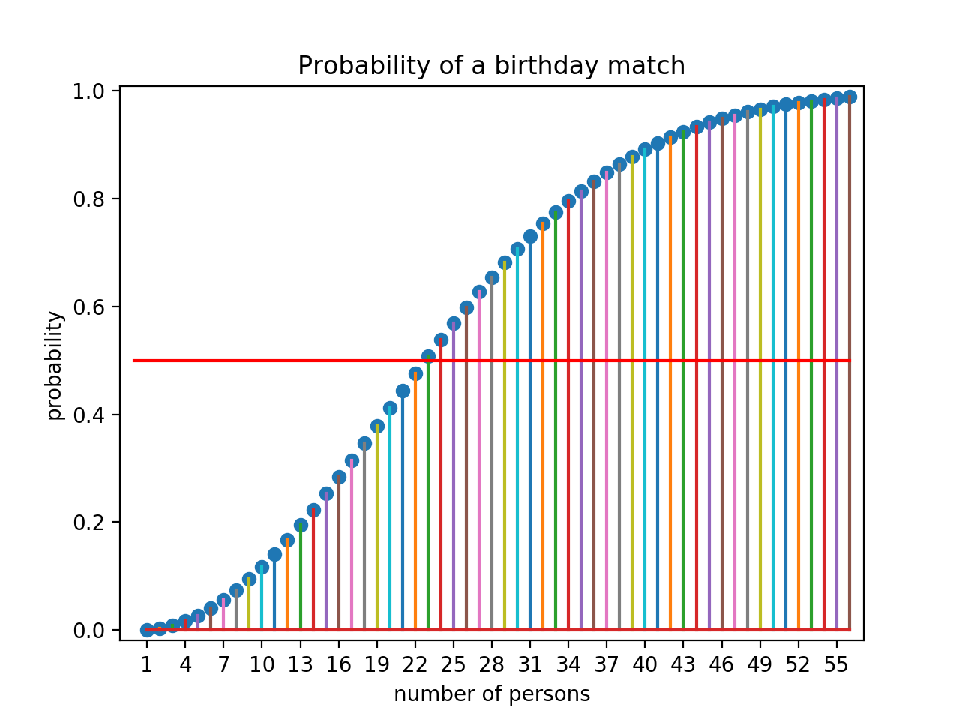
\epsfig{file=Abbildungen/birthday.pdf,scale=1.0}
   \caption{Das Geburtstags-Problem.}
  \label{fig:birthday}
\end{figure}
\section{Die hypergeometrische Verteilung}
\exercise In einer Ameisen-Kolonie, in der $40\,000$ Ameisen leben, sind $1\,000$ Ameisen
mit Farbe markiert worden.  Ein Forscher f�ngt nun zuf�llig $200$ dieser Ameisen.
Berechnen Sie die Wahrscheinlichkeit, dass er genau $k$ markierte Tiere f�ngt.  Gehen Sie
dabei von einem gleichm��igen Wahrscheinlichkeits-Ma� aus, nehmen Sie also an, dass
die Wahrscheinlichkeit daf�r, dass eine Ameise gefangen wird, unabh�ngig von der
farblichen Markierung f�r alle Ameisen gleich gro� ist.  Tabellieren
Sie die Werte f�r  $k=0,\cdots,20$ und  tragen Sie die gefundenen Werte in einem Diagramm auf.

\solution Wir modellieren die Ameisen-Kolonie durch die Menge $M := \{1,\cdots,40\,000\}$.
Die Menge der farblich markierten Ameisen bezeichnen wir mit $F$. Wir legen willk�rlich
fest, dass die ersten Tausend Ameisen diejenigen Ameisen sind, die markiert sind. Also
gilt
\\[0.2cm]
\hspace*{1.3cm} $F := \{1,\cdots,1\,000\}$
\\[0.2cm]
Das der Aufgabe zugrunde liegende Zufalls-Experiment besteht darin, dass wir aus der Menge
$M$ eine Teilmenge der Gr��e $200$ ausw�hlen.  Damit l�sst sich die Ergebnis-Menge als
\\[0.2cm]
\hspace*{1.3cm} $\Omega := \bigl\{ A \in 2^M \;\big|\; |A| = 200 \}$
\\[0.2cm]
definieren.  $\Omega$ ist also die Menge aller der Teilmengen von $M$, die genau $200$
Elemente enthalten.  Nach Gleichung (\ref{eq:kombination}) gilt f�r die M�chtigkeit dieser
Menge
\\[0.2cm]
\hspace*{1.3cm} $\ds |\Omega| = |C(M,200)| = {|M| \choose 200} = {40\,000 \choose 200}$
\\[0.2cm]
Das uns interessierende Ereignis $\Lambda_k$ ist das Ereignis, bei dem genau $k$ farblich markierte Ameisen
gefangen werden.  Wir k�nnen daher $\Lambda_k$ als
\\[0.2cm]
\hspace*{1.3cm} $\Lambda_k := \bigl\{ B \in 2^M \;\big|\; |B| = 200 \wedge |B \cap F| = k
\bigr\}$
\\[0.2cm]
definieren: $\Lambda_k$ besteht aus genau den Teilmengen von $M$, die einerseits 200 Elemente
enthalten und die andererseits genau $k$ Elemente aus der Menge $\{1,\cdots,1\,000\}$
enthalten.  Die Berechnung der Wahrscheinlichkeit des Ereignisses $\Lambda_k$ l�uft auf die
Berechnung von $|\Lambda_k|$ hinaus.  
Dazu formen wir die Definition von $\Lambda_k$ etwas um.  Eine Menge $B$ liegt genau dann
in $\Lambda_k$, wenn $B$ insgesamt $k$ Elemente aus der Menge $F$ und 
$200 - k$ Elemente aus der Menge $M \backslash F$ enth�lt.  Folglich gilt 
\\[0.2cm]
\hspace*{1.3cm}
$
\begin{array}{lcl}
|\Lambda_k| & = & 
\bigl|\bigl\{ C \cup D \bigm| C \subseteq F \wedge D \subseteq M \backslash F \wedge |C| = k \wedge |D| = 200 - k \bigr\}\bigr| \\[0.2cm]
 & = & 
\Bigl|\Bigl\{ C \cup D \Bigm| 
     C \in \bigl\{ C' \in 2^F \bigm| |C'| = k \bigr\}\; \wedge\; D \in \bigl\{ D' \in 2^{M \backslash F} \bigm| |D'| = 200 - k\bigr\} \Bigr\}\Bigr| \\[0.2cm]
 & = & 
\bigl|\{ C' \in 2^F \bigm| |C'| = k \}\bigr| \cdot \bigl|\{ D' \in 2^{M \backslash F} \bigm| |D'| = 200 - k\} \bigr| \\[0.2cm]
 & = & \ds
{|F| \choose k} \cdot {|M \backslash F| \choose 200 - k} \qquad \mbox{nach Gleichung   (\ref{eq:kombination})} \\[0.4cm] 
 & = & \ds
{1000 \choose k} \cdot {39\,000 \choose 200 - k}.  
\end{array}
$
\\[0.2cm]
Damit haben wir f�r die Wahrscheinlichkeit des Ereignisses $\Lambda_k$ die Formel 
\\[0.2cm]
\hspace*{1.3cm}
$\ds P(\Lambda_k) = \frac{|\Lambda_k|}{|\Omega|} =
     \frac{\ds{1000 \choose k} \cdot {39\,000 \choose 200 - k}}{\ds {40\,000 \choose 200}}
$
\\[0.2cm]
gefunden.  In Tabelle \ref{tab:ameisen} sind die Wahrscheinlichkeiten aufgelistet.
F�r $k\geq 17$ sinkt die Wahrscheinlichkeit unter $10^{-5}$ und ist damit vernachl�ssigbar.


\begin{table}[!ht]
  \centering
\framebox{
  \begin{tabular}{|r|r|r|r|r|r|}
\hline
   $k$ & $P(\Lambda_k)$ & $n$ & $P(\Lambda_k)$ & $k$ & $P(\Lambda_k)$ \\
\hline
\hline
  0 & 0.0062425837 &  1 & 0.0321774371 &  2 & 0.0824301154 \\
\hline
  3 & 0.1399249245 &  4 & 0.1770598037 &  5 & 0.1781466648 \\
\hline
  6 & 0.1484517284 &  7 & 0.1053817150 &  8 & 0.0650519877 \\
\hline
  9 & 0.0354730483 & 10 & 0.0173006288 & 11 & 0.0076226006 \\
\hline
 12 & 0.0030592431 & 13 & 0.0011261811 & 14 & 0.0003825168 \\
\hline
 15 & 0.0001204896 & 16 & 0.0000353530 & 17 & 0.0000096999 \\
\hline
  \end{tabular}}
  \caption{Wie viele markierte Ameisen werden gefangen?}
  \label{tab:ameisen}
\end{table}


\begin{figure}[!ht]
  \centering
   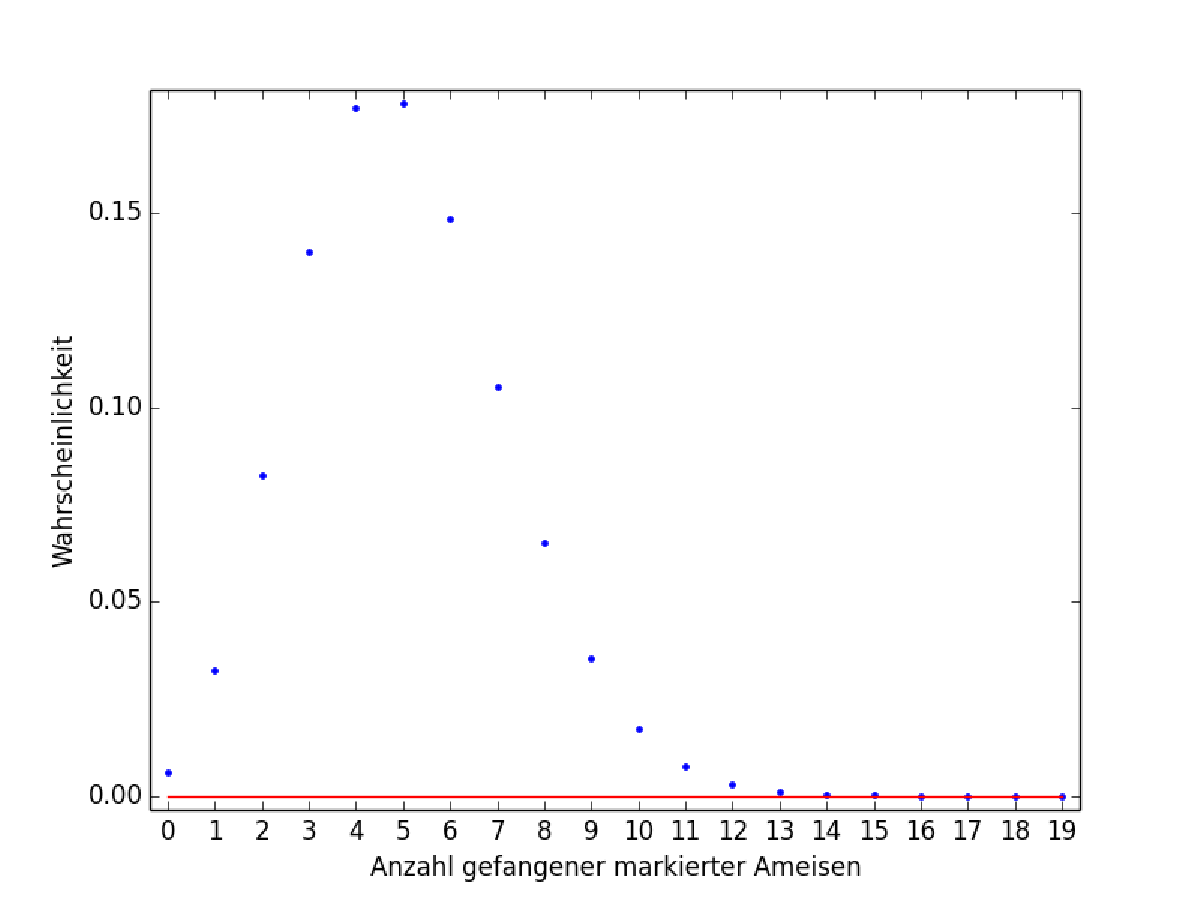
\epsfig{file=Abbildungen/ants.pdf,scale=0.5}
   \caption{Die Wahrscheinlichkeit, $k$ markierte Ameisen zu fangen.}
  \label{fig:ameisen}
\end{figure}


Die in der letzten Aufgabe behandelte Situation kommt in der Praxis h�ufig vor.
Ein Beispiel liefert die �berwachung der Qualit�t der Produktion von elektronischen
Bauteilen.  Eine Fertigungsanlage produziert am Tag eine bestimmte Zahl $N$ solcher 
Bauteile.  Davon sind $K$ Bauteile defekt, w�hrend die restlichen $N-K$
Bauteile funktionieren.  Zur �berpr�fung der Produktions-Qualit�t wird eine \blue{Stichprobe} vom
Umfang $n$ genommen.  In dieser Stichprobe findet man dann $k$ defekte Bauteile, w�hrend
die restlichen $n-k$ Bauteile einwandfrei sind.  Falls die Zahlen $N$, $K$ und $n$ gegeben sind, k�nnen
wir uns fragen, wie wahrscheinlich es ist, dass unter den $n$ Bauteilen der Stichprobe
insgesamt $k$ Bauteile defekt sind.  Die Situation ist dann dieselbe wie in der letzten
Aufgabe:  
\begin{enumerate}
\item Die Gesamtzahl $N$ entspricht der Anzahl aller Ameisen.
\item Die Anzahl $K$ der defekten Bauteile entspricht der Zahl der markierten Ameisen.
\item Die Umfang $n$ der Stichprobe entspricht der Zahl der gefangenen  Ameisen.
\item Die Anzahl $k$ der defekten Bauteile in der Stichprobe entspricht der Anzahl
      der gefangenen Ameisen, die markiert sind.
\end{enumerate}
Zur Berechnung des Wahrscheinlichkeits-Ma�es gehen wir daher wie bei der L�sung der
letzten Aufgabe vor und definieren  die Menge $\mathcal{M} := \{1,\cdots,N\}$, wobei wir die Bauteile
durchnummerieren und also jedes Bauteil durch eine Zahl der Menge $\mathcal{M}$ darstellen.
Die Menge der defekten Bauteile bezeichnen wir mit $\mathcal{F}$. 
Wir gehen ohne Beschr�nkung der Allgemeinheit davon aus, dass die defekten Bauteile in der
Aufz�hlung aller Bauteile am Anfang stehen, die Bauteile mit den Nummern
$1,\cdots,K$ sind also defekt.  Folglich gilt
\\[0.2cm]
\hspace*{1.3cm} $\mathcal{F} = \{1,\cdots,K\}$.
\\[0.2cm]
Das der Aufgabe zugrunde liegende Zufalls-Experiment besteht darin, dass wir aus der Menge
$\mathcal{M}$ eine Teilmenge der Gr��e $n$ ausw�hlen.  Damit l�sst sich die Ergebnis-Menge als
\\[0.2cm]
\hspace*{1.3cm} $\Omega = \bigl\{ A \in 2^\mathcal{M} \;\big|\; |A| = n \}$
\\[0.2cm]
Nach Gleichung (\ref{eq:kombination}) gilt f�r die M�chtigkeit dieser Menge
\\[0.2cm]
\hspace*{1.3cm} $\ds |\Omega| = |C(\mathcal{M},n)| = {|\mathcal{M}| \choose n} = {N \choose n}$
\\[0.2cm]
Das uns interessierende Ereignis $\Lambda_k$ ist dann durch die Menge
\\[0.2cm]
\hspace*{1.3cm} 
$\Lambda_k := \bigl\{ B \in 2^\mathcal{M} \;\big|\; |B| = n \wedge |B \cap \mathcal{F}| = k\bigr\}$
\\[0.2cm]
definiert: $\Lambda_k$ besteht aus genau den Teilmengen von $\mathcal{M}$, die  $n$ Elemente
enthalten von denen $k$ defekt sind.  Die Berechnung der Wahrscheinlichkeit des Ereignisses $\Lambda_k$ l�uft
auf die Berechnung von $|\Lambda_k|$ hinaus.  
Dazu formen wir die Definition von $\Lambda_k$ etwas um.  Eine Menge $B$ liegt genau dann
in $\Lambda_k$, wenn $B$ insgesamt $k$ Elemente aus der Menge $\mathcal{F}$ und 
$n - k$ Elemente aus der Menge $\mathcal{M} \backslash \mathcal{F}$ enth�lt.  Folglich gilt 
\\[0.2cm]
\hspace*{1.3cm}
$
\begin{array}{lcl}
|\Lambda_k| & = & 
\bigl|\bigl\{ C \cup D \bigm| C \subseteq \mathcal{F} \wedge D \subseteq \mathcal{M} \backslash \mathcal{F} \wedge |C| = k \wedge |D| = n - k \bigr\}\bigr| \\[0.2cm]
 & = & 
\bigl|\bigl\{ C \cup D \bigm| C \in \{ C' \in 2^\mathcal{F} \bigm| |C'| = k \}\; \wedge\; D \in \{ D' \in 2^{\mathcal{M} \backslash \mathcal{F}} \bigm| |D'| = n - k\} \bigr\}\bigr| \\[0.2cm]
 & = & 
\bigl|\{ C' \in 2^\mathcal{F} \bigm| |C'| = k \}\bigr| \cdot \bigl|\{ D' \in 2^{\mathcal{M} \backslash \mathcal{F}} \bigm| |D'| = n - k\} \bigr| \\[0.2cm]
 & = & \ds
{|\mathcal{F}| \choose k} \cdot {|\mathcal{M} \backslash \mathcal{F}| \choose n - k} \qquad \mbox{nach Gleichung   (\ref{eq:kombination})} \\[0.4cm] 
 & = & \ds
{n \choose k} \cdot {N - K \choose n - k}.  
\end{array}
$
\\[0.2cm]
Damit haben wir f�r das Wahrscheinlichkeits-Ma� die Formel 
\begin{equation}
  \label{eq:hypergeometrisch}  
 P(\Lambda_k) = \frac{|\Lambda_k|}{|\Omega|} =\frac{\ds{K \choose k} \cdot {N - K \choose n - k}}{\ds{N \choose n}}
\end{equation}
gefunden.  In der Statistik wird das obige Beispiel abstrahiert.  Statt von Bauteilen
sprechen wir hier von Kugeln in einer Urne.  Von diesen Kugeln sind dann $K$ Kugeln
schwarz, was den defekten Bauteilen entspricht, die restlichen Kugeln sind wei�.
Dann gibt die obige Formel die Wahrscheinlichkeit daf�r an, dass bei einer Entnahme von
$n$ Kugeln $k$ Kugeln schwarz sind.  Das in Gleichung \ref{eq:hypergeometrisch} angegebene
Wahrscheinlichkeits-Ma� wird in der Literatur als 
\href{https://de.wikipedia.org/wiki/Hypergeometrische_Verteilung}{hypergeometrische Verteilung}
bezeichnet. 

\exercise
Eine Firma erh�lt eine Lieferung von 100 Ger�ten.  Der zust�ndige Pr�fer w�hlt zuf�llig 10
Ger�te aus.  Die Lieferung wird genau dann akzeptiert, wenn dabei kein defektes Ger�t
gefunden wird.  Nehmen Sie an, dass von den gelieferten 100 Ger�ten 10 Ger�te defekt sind.
Wie hoch ist die Wahrscheinlichkeit daf�r, dass die Lieferung trotzdem akzeptiert wird?

\section{Die Binomial-Verteilung}
Wir greifen das Beispiel aus der Einleitung zur Ameisen-Z�hlung wieder auf und
modifizieren es mit dem Ziel, die Durchf�hrung zu vereinfachen:
\begin{enumerate}
\item Am ersten Tag markieren wir wie vorher insgesamt $1\,000$ Ameisen farblich.
\item Der zweite Tag ist schwieriger, denn hier m�ssten wir tats�chlich erst  $200$
      Ameisen einsammeln bevor wir mit dem Z�hlen der markierten Ameisen beginnen.
      Also �ndern wir das Experiment so ab, dass wir nacheinander $200$ Ameisen
      untersuchen und jedes Mal �berpr�fen, ob die Ameise markiert ist.  
\end{enumerate}
Am zweiten Tag kann es jetzt durchaus passieren, dass wir dieselbe Ameise mehrmal z�hlen.
Dadurch �ndert sich nat�rlich auch das Wahrscheinlichkeits-Ma�.  Wenn wir berechnen
wollen, mit welcher Wahrscheinlichkeit wir nun $k$ markierte Ameisen finden, 
werden die Dinge erfreulicherweise einfacher.  Wir behandeln gleich den allgemeinen Fall
und nehmen folgendes an:
\begin{enumerate}
\item F�r jede einzelne Ameise hat die Wahrscheinlichkeit, dass die Ameise markiert ist,
      den Wert \\[0.2cm]
      \hspace*{1.3cm}
      $\ds p = \frac{K}{N}$.
      \\[0.2cm]
      Hier bezeichnet $N$ die Gesamtzahl der Ameisen und $K$ ist die Anzahl der insgesamt
      markierten Ameisen.  Die Menge $\mathcal{M}$  der Ameisen hat also die Form 
      \\[0.2cm]
      \hspace*{1.3cm}
      $\{ a_1,a_2,\cdots,a_N\}$
      \\[0.2cm]
      Ohne Beschr�nkung der Allgemeinheit gehen wir davon aus, dass die Ameisen
      $a_1$ bis $a_K$ markiert sind.
\item Das Zufalls-Experiment besteht darin, dass wir $n$ Ameisen auf ihre F�rbung
      untersuchen.  Dabei erhalten wir als Ergebnis eine Liste $[x_1,x_2,\cdots,x_n]$
      von Ameisen.   Stellen wir die Ameisen durch nat�rliche Zahlen von $1$ bis $N$ dar,
      so gilt also $x_i \in \{a_1,\cdots,a_N\}$.
\end{enumerate}
Da Listen der L�nge $n$ nichts anderes als $n$-Tupel sind, ist  die Ergebnis-Menge unseres
Zufalls-Experiments also das $n$-fache kartesische Produkt der Menge $\mathcal{M}$:
\\[0.2cm]
\hspace*{1.3cm}
$\Omega = \mathcal{M}^n$.
\\[0.2cm]
Nach Gleichung (\ref{eq:tupel-wiederholung}) folgt daraus 
\\[0.2cm]
\hspace*{1.3cm}
$|\Omega| = |\mathcal{M}|^n = N^n$.
\\[0.2cm]
Wir definieren nun $\Lambda_k$ als die Menge aller $n$-Tupel, die aus $k$ markierten
Ameisen bestehen.  Wir denken uns ein solches $n$-Tupel aus zwei Teilen bestehend:
 einem $k$-Tupel von markierten Ameisen und einem $(n-k)$-Tupel von unmarkierten Ameisen.  Es gibt insgesamt
$K^k$ solcher $k$-Tupel und $(N-K)^{n-k}$ solcher $(n-k)$-Tupel.
Als n�chstes �berlegen wir uns, wieviele M�glichkeiten es gibt, aus einem 
$k$-Tupel und einem $(n-k)$-Tupel ein $n$-Tupel zu erzeugen.  
Betrachten wir zun�chst ein konkretes Beispiel: Um aus dem $3$-Tupel $[x_1,x_2,x_3]$ und 
dem $2$-Tupel $[y_1,y_2]$  ein $5$-Tupel zu erstellen m�ssen wir die Menge $I$ der Indizes
festlegen, an denen wir die Elemente $x_i$ einf�gen.  Setzen wir beispielsweise $I:=
\{1,2,3\}$, so w�rden die Elemente $x_i$ am Anfang stehen und wir h�tten 
\\[0.2cm]
\hspace*{1.3cm}
$I = \{1,2,3\}$: \qquad $[x_1,x_2,x_3,y_1,y_2]$.
\\[0.2cm]
F�r $I = \{1,3, 4\}$ w�rde sich 
\\[0.2cm]
\hspace*{1.3cm}
$I = \{1,3,4\}$: \qquad $[x_1,y_1,x_2,x_3,y_2]$.
\\[0.2cm]
ergeben.  Jede solche Index-Menge $I \subseteq \{1,\cdots,5\}$ legt also eindeutig fest,
wie wir aus den beiden Tupeln ein $5$-Tupel bilden k�nnen.

Im allgemeinen Fall gilt einerseits $I \subseteq \{1,\cdots,n\}$ und andererseits $|I| =
k$.  Damit ist $I$ dann eine $k$-elementige Teilmenge einer $n$-elementigen Menge.   Nach
Gleichung (\ref{eq:kombination}) gilt also 
\\[0.2cm]
\hspace*{1.3cm}
$\ds |I| = {n \choose k}$.
\\[0.2cm]
Damit ergibt sich f�r die M�chtigkeit des Ereignisses $\Lambda_k$ der folgende Ausdruck 
\\[0.2cm]
\hspace*{1.3cm}
$\ds |\Lambda_k| = |I| \cdot K^k \cdot (N-K)^{n-k} = {n \choose k} \cdot K^k \cdot (N-K)^{n-k}$.
\\[0.2cm]
Die Wahrscheinlichkeit, dass wir $k$ markierte Ameisen z�hlen, ergibt sich jetzt zu 
\\[0.2cm]
\hspace*{1.3cm}
$
\begin{array}[b]{lcll}
 P(k) := P(\Lambda_k) & = & \ds \frac{|\Lambda_k|}{|\Omega|} \\[0.4cm]
 & = & \ds \frac{\ds{n \choose k} \cdot K^k \cdot (N-K)^{n-k}}{N^n} \\[0.4cm]
 & = & \ds {n \choose k} \cdot \frac{K^k}{N^k} \cdot \frac{(N-K)^{n-k}}{N^{n-k}} \\[0.4cm]
 & = & \ds {n \choose k} \cdot \left(\frac{K}{N}\right)^k \cdot \left(1 - \frac{K}{N}\right)^{n-k} \\[0.4cm]
 & = & \ds {n \choose k} \cdot p^k \cdot \left(1 - p\right)^{n-k} & \ds \mbox{mit} \quad p := \frac{K}{N}
\end{array}
$
\\[0.2cm]
Wir abstrahieren nun von den Ameisen und fassen unsere Ergebnisse wie folgt zusammen.  Ist
ein Zufalls-Experiment dadurch gekennzeichnet, dass $n$ mal ein Experiment durchgef�hrt
wird, bei dem es nur zwei m�gliche Ergebnisse gibt, die wir jetzt mit $a$ und $b$
bezeichnen und hat die Wahrscheinlichkeit f�r das Auftreten von $a$ bei jedem solchen
Experiment den selben Wert 
$p$, dann ist die Wahrscheinlichkeit daf�r, dass bei einer $n$-fachen Durchf�hrung dieses
Experiments $k$ mal das Ergebnis $a$ auftritt, durch 
\begin{equation}
  \label{eq:binomial}
  P(k) = {n \choose k} \cdot p^k \cdot (1-p)^{n-k}
\end{equation}
gegeben.  Diese Wahrscheinlichkeits-Funktion bezeichnen wir als \blue{Binomial-Verteilung}
und definieren 
\\[0.2cm]
\hspace*{1.3cm}
$\ds \mathrm{Bin}(n,k;p) := {n \choose k} \cdot p^k \cdot (1-p)^{n-k}$.

\section{Zufalls-Variablen}
Es wird Zeit, dass wir einen Begriff formal definieren, der uns in verschiedenen
Beispielen schon mehrfach begegnet ist.  Dies ist der Begriff der \blue{Zufalls-Variable}.

\begin{Definition}[Zufalls-Variable]
Es sei ein Wahrscheinlichkeits-Raum $\langle \Omega, 2^\Omega, P \rangle$ gegeben. 
Eine Funktion 
\\[0.0cm]
\hspace*{1.3cm}
$X:\Omega \rightarrow \mathbb{R}$
\\[0.2cm]
bezeichnen wir als \href{https://de.wikipedia.org/wiki/Zufallsvariable}{Zufalls-Variable}. \qed
\end{Definition}

\example
Ein einfaches Beispiel f�r eine Zufalls-Variable w�re die Summe $S$ der Augenzahlen, wenn mit zwei
W�rfeln gew�rfelt wird.  Der Ergebnis-Raum $\Omega$ ist in diesem Fall
\\[0.2cm]
\hspace*{1.3cm}
$\Omega = \bigl\{ \langle i, j \rangle \bigm| i,j \in \{1,\cdots,6\}\bigr\}$.
\\[0.2cm]
Wenn wir davon ausgehen, dass es sich bei den W�rfeln um Laplace-W�rfel handelt, dann
ist die Wahrscheinlichkeits-Verteilung $P: 2^\Omega \rightarrow \mathbb{R}$ durch die Formel 
\\[0.2cm]
\hspace*{1.3cm}
$\ds P(A) = \frac{|A|}{|\Omega|} = \frac{1}{36} \cdot |A|$
\\[0.2cm]
gegeben.  Die Zufalls-Variable $S: \Omega \rightarrow \mathbb{R}$ definieren wir durch 
\\[0.2cm]
\hspace*{1.3cm}
$S\bigl(\langle i,j \rangle\bigr) := i + j$.
\\[0.2cm]
Wenn uns die Wahrscheinlichkeit f�r das Auftreten einer bestimmten Augensumme
interessiert, dann m�ssen wir zun�chst die diesbez�glichen Ereignisse definieren.
Bei diesen Ereignissen handelt es sich um die Mengen 
\\[0.2cm]
\hspace*{1.3cm}
$\bigl\{ \langle i,j \rangle \in \Omega \;\big|\; i + j = s \}$ \quad f�r $s=2,\cdots,12$.
\\[0.2cm]
Ist $X$ eine Zufalls-Variable, die auf einem Ergebnis-Raum $\Omega$ definiert ist, so
vereinbaren wir zur Abk�rzung die folgende Schreibweise:  
\\[0.2cm]
\hspace*{1.3cm}
$P(X = x) := P\bigl(\{ \omega \in \Omega \;|\; X(\omega) = x\}\bigr)$.
\\[0.2cm]
In unserem konkreten Beispiel schreiben wir also 
\\[0.2cm]
\hspace*{1.3cm}
$P(S = s) = P\bigl(\{ \langle i,j \rangle \in \Omega \;|\; i+j = s \}\bigr)$.
\\[0.2cm]
F�r $s \leq 7$ gilt 
\\[0.2cm]
\hspace*{1.3cm}
$\bigl\{ \langle i,j \rangle \in \Omega \;\big|\; i + j = s \} = 
 \bigl\{ \langle k, s - k \rangle \;|\; k \in \{1,\cdots,s-1\}\bigr\}$.
\\[0.2cm]
Die Bedingung $k \leq s-1$ folgt aus der Ungleichung $1 \leq s - k$.
F�r $s > 7$ finden wir
\\[0.2cm]
\hspace*{1.3cm}
$\bigl\{ \langle i,j \rangle \in \Omega \;\big|\; i + j = s \} = 
 \bigl\{ \langle 7 - k, s - 7 + k \rangle \;|\; k \in \{1,\cdots,13 -s\}\bigr\}$.
\\[0.2cm]
Die Bedingung $k \leq 13-s$ folgt dabei aus der Forderung $s - 7 + k \leq 6$.
Daraus ergibt sich 
\\[0.2cm]
\hspace*{1.3cm}
$\bigl|\bigl\{ \langle i,j \rangle \in \Omega \;\big|\; i + j = s \}\bigr| \,=\,  \left\{
\begin{array}{ll}
  s-1  & \mbox{falls $s \leq 7$}; \\
  13-s & \mbox{sonst}.
\end{array}
\right.
$
\\[0.2cm]
Also haben wir
\\[0.2cm]
\hspace*{1.3cm}
$P(S = s) = \left\{
\begin{array}{ll}
\ds  \frac{s-1}{36}  & \mbox{falls $s \leq 7$}; \\[0.5cm]
\ds  \frac{13-s}{36} & \mbox{sonst}.
\end{array}
\right.
$
\\[0.2cm]
Die Funktion $s \mapsto P(S = s)$ bezeichnen wir als \blue{Wahrscheinlichkeits-Funktion}
der Zufalls-Variablen $S$.  Wir schreiben diese Funktion als $f_s$, es gilt also
\\[0.2cm]
\hspace*{1.3cm}
$f_S(s) = P(S = s)$.
\\[0.2cm]
Wir sehen hier, dass die Wahrscheinlichkeit f�r die verschiedenen m�glichen Werte der
Summe $S$ nicht mehr gleichm��ig verteilt sind, obwohl die Wahrscheinlichkeits-Verteilung
$P$ auf dem zugrunde liegenden Wahrscheinlichkeits-Raum sehr wohl gleichm��ig ist.
Die Ursache hierf�r ist einfach einzusehen: Es gibt beispielsweise 6 M�glichkeiten, in der
Summe eine 6 zu w�rfeln, aber es gibt nur eine einzige M�glichkeit um in der Summe eine 12
zu w�rfeln.

\begin{figure}[!ht]
  \centering
   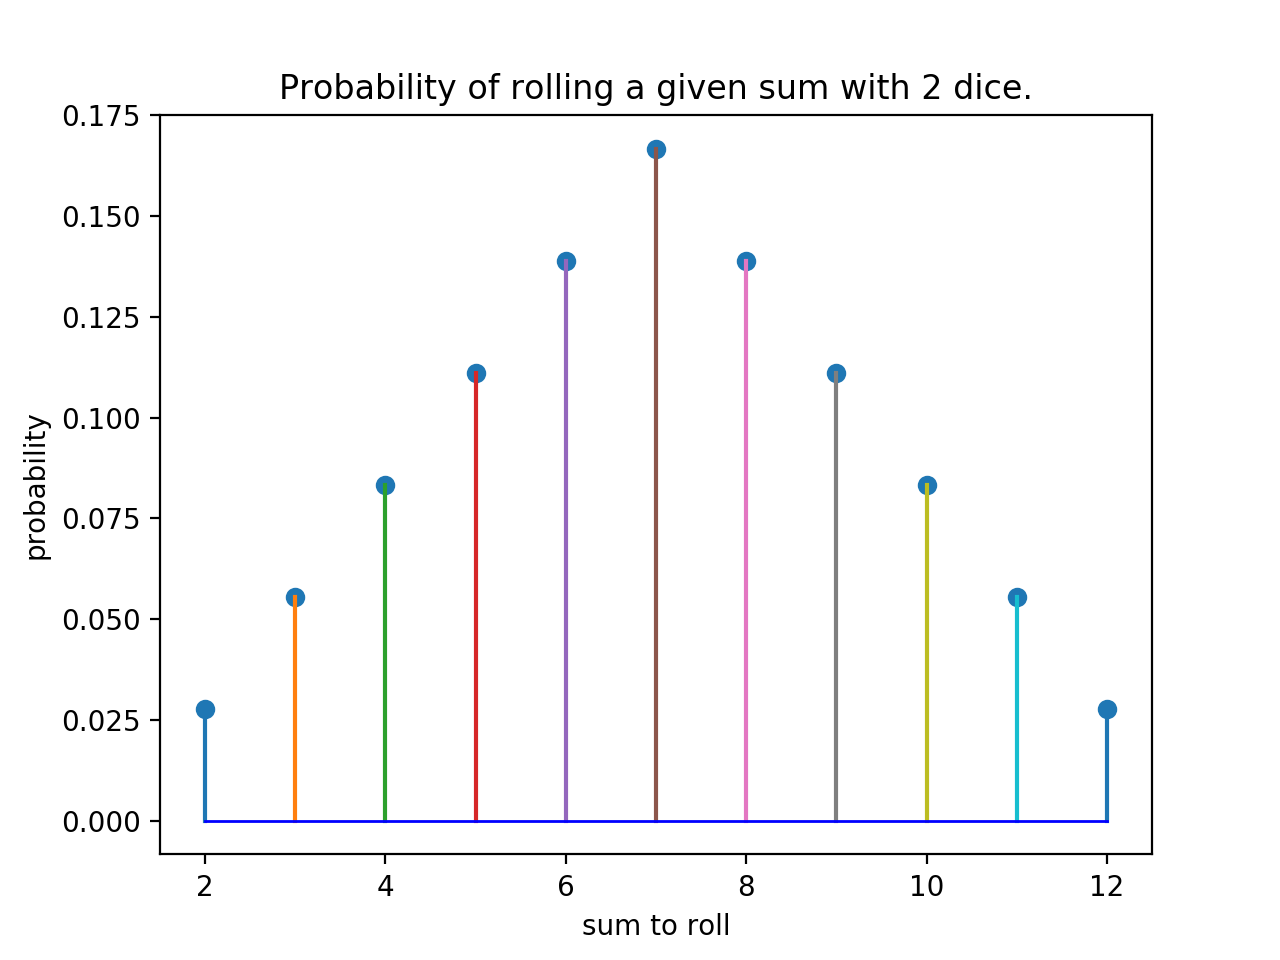
\epsfig{file=Abbildungen/dice-2, scale=1.0}
   \caption{Wahrscheinlichkeits-Funktion der Zufalls-Variablen $S$}
  \label{fig:dice-2}
\end{figure}

\begin{Definition}[Wahrscheinlichkeits-Funktion]
  Ist $\langle \Omega, 2^\Omega, P \rangle$ ein diskreter Wahrscheinlichkeits-Raum und ist $X:\Omega \rightarrow \mathbb{R}$ 
  eine Zufalls-Variablen, so bezeichnen wir die Funktion
  \\[0.2cm]
  \hspace*{1.3cm}
  $f_X:\mathrm{range}(X) \rightarrow [0,1]$,
  \\[0.2cm]
  die durch die Gleichung
  \\[0.2cm]
  \hspace*{1.3cm}
  $f_X(x) := P(X = x)$
  \\[0.2cm]
  definiert ist, als die der Zufalls-Variablen $X$ zugeordnete \blue{Wahrscheinlichkeits-Funktion}.  \eoxs
\end{Definition}

\example
Bei dem letzten Beispiel haben wir die Summe $S$ der Augenzahlen beim W�rfeln mit zwei W�rfeln als
Zufalls-Variable betrachtet.  F�r die Zufalls-Variable $S$ gilt in diesem Fall
\\[0.2cm]
\hspace*{1.3cm}
$\mathrm{range}(S) = \{2, \cdots, 12\}$,
\\[0.2cm]
denn die Summe der Augenzahl beim W�rfeln mit zwei W�rfeln ist mindestens 2 und h�chstens 12.  F�r die
Wahrscheinlichkeits-Funktion $f_S$ gilt nach dem, was wir oben ausgerechnet haben:
\\[0.2cm]
\hspace*{1.3cm}
$f_S(k) = \left\{
\begin{array}{ll}
\ds  \frac{k-1}{36}  & \mbox{falls $k \leq 7$}; \\[0.5cm]
\ds  \frac{13-k}{36} & \mbox{sonst}. 
\end{array}
\right.
$ 
\\[0.2cm]
Die Wahrscheinlichkeits-Funktion $f_s$ ist in Abbildung \ref{fig:dice-2} gezeigt.  \eoxs

\remark
Ist $\langle \Omega, 2^\Omega, P \rangle$ ein diskreter Wahrscheinlichkeits-Raum, ist $X:\Omega \rightarrow \mathbb{R}$ 
eine Zufalls-Variable mit $\mathrm{range}(X) = \{x_1, \cdots, x_n\}$ und hat $X$ die Wahrscheinlichkeits-Funktion $f_X$, so muss
\\[0.2cm]
\hspace*{1.3cm}
$\ds \sum\limits_{i=1}^n f_X(x_i) = 1$
\\[0.2cm]
gelten, denn aus der Gleichung $\mathrm{range}(X) = \{x_1, \cdots, x_n\}$ folgt, dass das Ereignis
\\[0.2cm]
\hspace*{1.3cm}
$\ds \bigcup\limits_{i=1}^n \bigl\{ \omega \in \Omega \bigm| X(\omega) = x_i \bigr\}$ 
\\[0.2cm]
mit dem Ergebnis-Raum $\Omega$ identisch ist und folglich die Wahrscheinlichkeit $1$ hat.
Da wir andererseits
\\[0.2cm]
\hspace*{1.3cm}
$f_X(x_i) = P\bigl(\bigl\{ \omega \in \Omega \bigm| X(\omega) = x_i \bigr\}\bigr)$
\\[0.2cm]
haben, muss die Summe dieser Wahrscheinlichkeiten den Wert $1$ ergeben.  \eox

\exercise Betrachten Sie allgemein den Fall, dass mit $n$ W�rfeln gew�rfelt wird.  Der
Ergebnis-Raum $\Omega$ ist dann das $n$-fache kartesische Produkt der Menge
$\{1,\cdots,6\}$:
\\[0.2cm]
\hspace*{1.3cm} $\ds \Omega = \{ 1,\cdots,6 \}^n$
\\[0.2cm]
Berechnen Sie mit Hilfe eines geeigneten Programms (in einer Programmiersprache ihrer
Wahl) die Wahrscheinlichkeit daf�r, dass die Augensumme aller W�rfel den Wert $s$ hat und
erstellen Sie den Graphen der Funktion
\\[0.2cm]
\hspace*{1.3cm}
$P_n: \{n, \cdots, 6 \cdot n\} \rightarrow \mathbb{R}$
\\[0.2cm]
die durch
\\[0.2cm]
\hspace*{1.3cm}
$\ds P_n(s) = P\Bigl(\bigl\{\langle x_1,\cdots,x_n\rangle \in \Omega \;\big|\;s =
  \sum\limits_{i=1}^n x_i \bigr\}\Bigl)$.
\\[0.2cm]
gegeben ist.  Zeichnen Sie diesen Graphen f�r die Werte $n=2$, $n=3$, $n=5$, $n=10$, sowie $n=100$.
\vspace*{0.2cm}

\noindent
\textbf{Hinweis}:  Sie k�nnen den Wert $P_n(s)$ nat�rlich mit dem W�rfel-Summen-Satz berechnen.  Allerdings
muss dann die von Ihnen verwendete Programmiersprache in der Lage sein, Ausdr�cke der Form ${n \choose k}$ auch
f�r sehr gro�e Werte von $n$ exakt berechnen zu k�nnen.  Wenn diese Voraussetzung nicht erf�llt ist, dann
k�nnen Sie $P_n(s)$ am besten rekursiv berechnen, indem Sie $P_n$ auf $P_{n-1}$ zur�ck f�hren.  Allerdings
sollten Sie sich dar�ber im Klaren sein, dass eine naive rekursive Implementierung nur f�r kleine Werte von $n$
in endlicher Zeit ein Ergebnis berechnet.
\eoxs

\begin{Definition}[Bernoulli-Verteilung]
Ist $\langle \Omega, 2^\Omega, P \rangle$ ein Wahrscheinlichkeits-Raum und ist $X$ eine Zufalls-Variable, die
nur die beiden Werte $0$ und $1$ annimmt, wobei der Wert $1$ mit der Wahrscheinlichkeit $p$ angenommen wird, gilt also
\\[0.2cm]
\hspace*{1.3cm}
$X: \Omega \rightarrow \{0,1\}$ \quad und \quad $P(X=1) = p$,
\\[0.2cm]
dann sagen wir, dass $X$ eine \href{https://de.wikipedia.org/wiki/Bernoulli-Verteilung}{Bernoulli-Verteilung}
(\href{https://de.wikipedia.org/wiki/Jakob_I._Bernoulli}{Jacob I. Bernoulli}, 1655 --- 1705)
mit Parameter $p$ hat und schreiben
\\[0.2cm]
\hspace*{1.3cm}
$X \sim \mathrm{Bern}(p)$ (lese: $X$ ist Bernoulli-verteilt mit Parameter $p$).  \eox
\end{Definition}

Hat ein Zufalls-Experiment nur zwei m�gliche Ausg�nge, von denen wir einen als \blue{Erfolg} und den anderen
als \blue{Misserfolg} bezeichnen, so k�nnen wir die Menge $\Omega$ als
\\[0.2cm]
\hspace*{1.3cm}
$\Omega := \{ \mathrm{E}, \mathrm{M} \}$
\\[0.2cm]
darstellen, wobei das Ergebnis $\mathrm{E}$ f�r ``Erfolg'' und das Ergebnis $\mathrm{M}$ f�r ``Misserfolg''
steht.  Definieren wir die Zufalls-Variable $X: \Omega \rightarrow \{0,1\}$  durch
\\[0.2cm]
\hspace*{1.3cm}
$X(\mathrm{E}) = 1$ \quad und \quad $X(\mathrm{M}) = 0$
\\[0.2cm]
und definieren wir weiter
\\[0.2cm]
\hspace*{1.3cm}
$p := P(\{\mathrm{E}\})$,
\\[0.2cm]
so gilt $X \sim \mathrm{Bern}(p)$.  Ein solches Zufalls-Experiment hei�t \blue{Bernoulli-Experiment} mit
Parameter $p$.  Ein einfaches Beispiel f�r ein solches Bernoulli-Experiment w�re der Wurf
einer M�nze, wenn wir beispielsweise ``Wappen'' als Erfolg und ``Zahl'' als Misserfolg interpretieren.
Wiederholen wir ein solches Bernoulli-Experiment mehrmals,  wobei die einzelnen Wiederholungen voneinander
unabh�ngig sind, und summieren wir dann die Anzahl der Erfolge,  so ist diese Summe eine Zufalls-Variable, die
einer \blue{Binomial-Verteilung} gen�gt.  Diesen Begriff definieren wir nun formal.

\begin{Definition}[Binomial-Verteilung]
  Wird ein Bernoulli-Experiment mit Parameter $p$ insgesamt $n$ mal so wiederholt, dass die einzelnen
  Ausf�hrungen des Experiments 
  voneinander unabh�ngig sind, und beschreibt die Zufalls-Variable $S$ die Anzahl der Erfolge, die sich bei der
  $n$-maligen Durchf�hrung des Bernoulli-Experiments ergeben, so sagen wir, dass die Zufalls-Variable $S$
  \blue{binomial mit den Parameter $n$ und $p$ verteilt} ist und schreiben
  \\[0.2cm]
  \hspace*{1.3cm}
  $S \sim \mathrm{Bin}(n, p)$.  \qed
\end{Definition}

Wir wollen nun die Wahrscheinlichkeits-Funktion einer binomial-verteilten Zufalls-Variable berechnen.  Dazu
definieren wir zun�chst den Ereignis-Raum $\Omega$ als die Menge aller $n$-Tupel, die nur die beiden Elemente
$\mathrm{E}$ (f�r ``Erfolg'') und $\mathrm{M}$ (f�r ``Misserfolg'') enthalten, es gilt also
\\[0.2cm]
\hspace*{1.3cm}
$\Omega = \{ \mathrm{E}, \mathrm{M}\}^n$.
\\[0.2cm]
Ist $p$ die Wahrscheinlichkeit daf�r, dass bei einem einzelnen der $n$ Bernoulli-Experimente ein Erfolg
eintritt, so h�ngt die Wahrscheinlichkeit $P(\omega)$ f�r $\omega \in \Omega$ davon ab, wie oft in der Liste
ein Erfolg bzw.~ein Misserfolg vorliegt.  Ist beispielsweise $n=5$ und betrachten wir das Elementar-Ereignis
\\[0.2cm]
\hspace*{1.3cm}
$A := \bigl\{[\mathrm{E}, \mathrm{M}, \mathrm{E}, \mathrm{E}, \mathrm{M}]\bigr\}$,
\\[0.2cm]
so gilt $P(A) = p^3 \cdot (1 - p)^2$, denn bei dem Ereignis $A$ sind $3$ der Bernoulli-Experimente erfolgreich,
w�hrend zwei der Bernoulli-Experimente nicht erfolgreich waren.  Ist allgemein $B$ ein Elementar-Ereignis, bei
dem $k$ der zugeh�rigen Bernoulli-Experimente erfolgreich und die restlichen $n-k$ Bernoulli-Experimente nicht
erfolgreich sind, so gilt
\\[0.2cm]
\hspace*{1.3cm}
$P(B) = p^k \cdot (1 - p)^{n-k}$.
\\[0.2cm]
Wir m�ssen uns nun fragen, wie viele Elementar-Ereignisse es in der Menge $\Omega$ gibt, bei denen genau $k$ der
insgesamt $n$ Bernoulli-Experimente erfolgreich sind.  Diese Zahl ist aber gleich der Anzahl der M�glichkeiten,
die wir haben, um aus einer $n$-elementigen Menge $k$ Elemente auszuw�hlen und diese Zahl ist gerade 
${n \choose k}$.  Damit haben wir die Wahrscheinlichkeits-Funktion einer binomial verteilten Zufalls-Variable
gefunden: Falls $S \sim \mathrm{Bin}(n,p)$ ist, so gilt
\\[0.2cm]
\hspace*{1.3cm}
$\ds f_S(k) = P(S = k) = {n \choose k} \cdot p^k \cdot (1 - p)^{n-k}$.
\\[0.2cm]
Die Abbildungen \ref{fig:bin10.png} und \ref{fig:bin100.png} auf Seite \pageref{fig:bin10.png} zeigen
verschiedene Binomial-Verteilungen.

\begin{figure}[!ht]
  \centering
   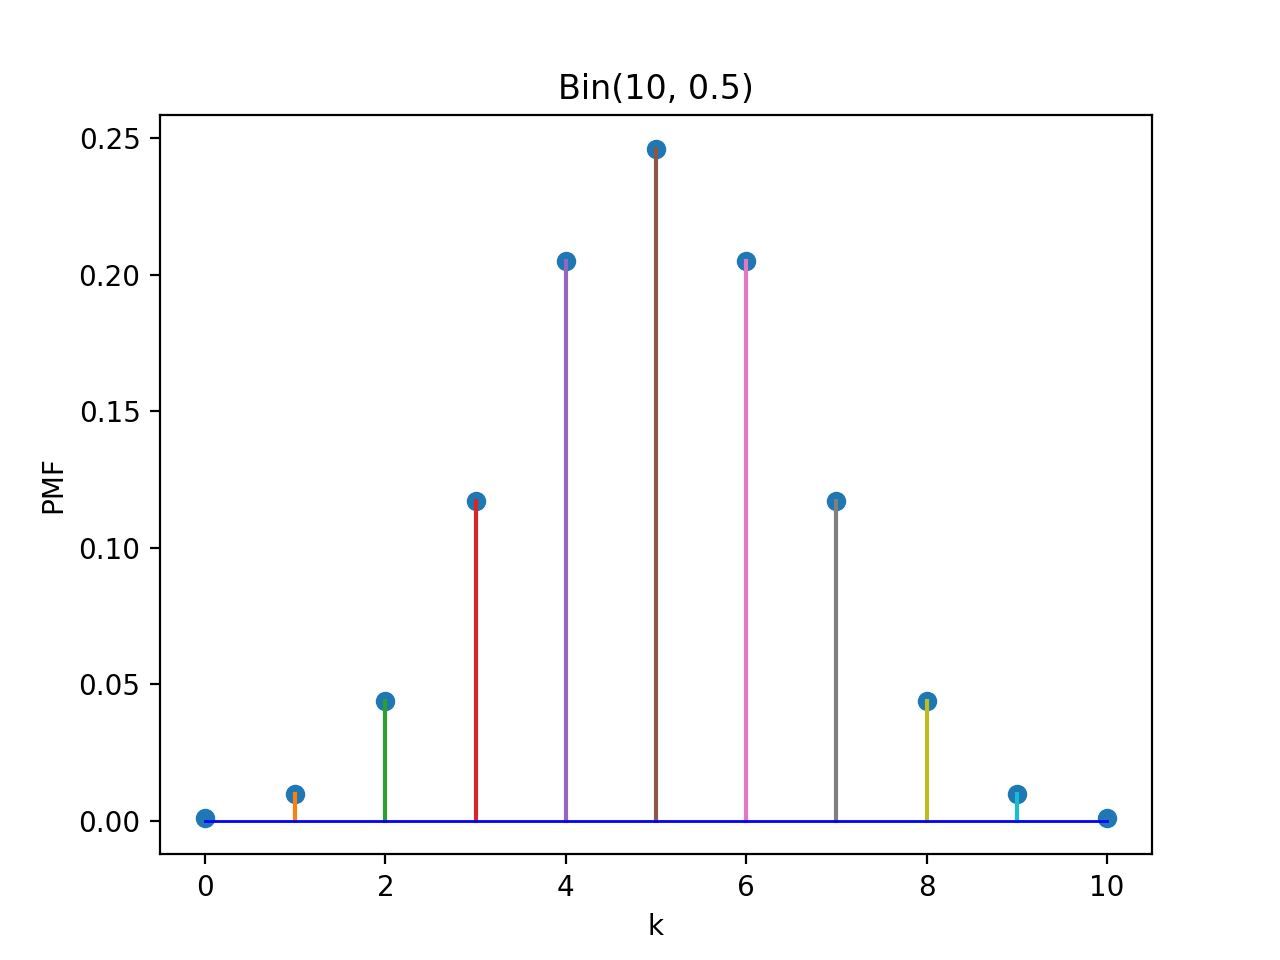
\epsfig{file=Abbildungen/bin10half.png, scale=0.45}
   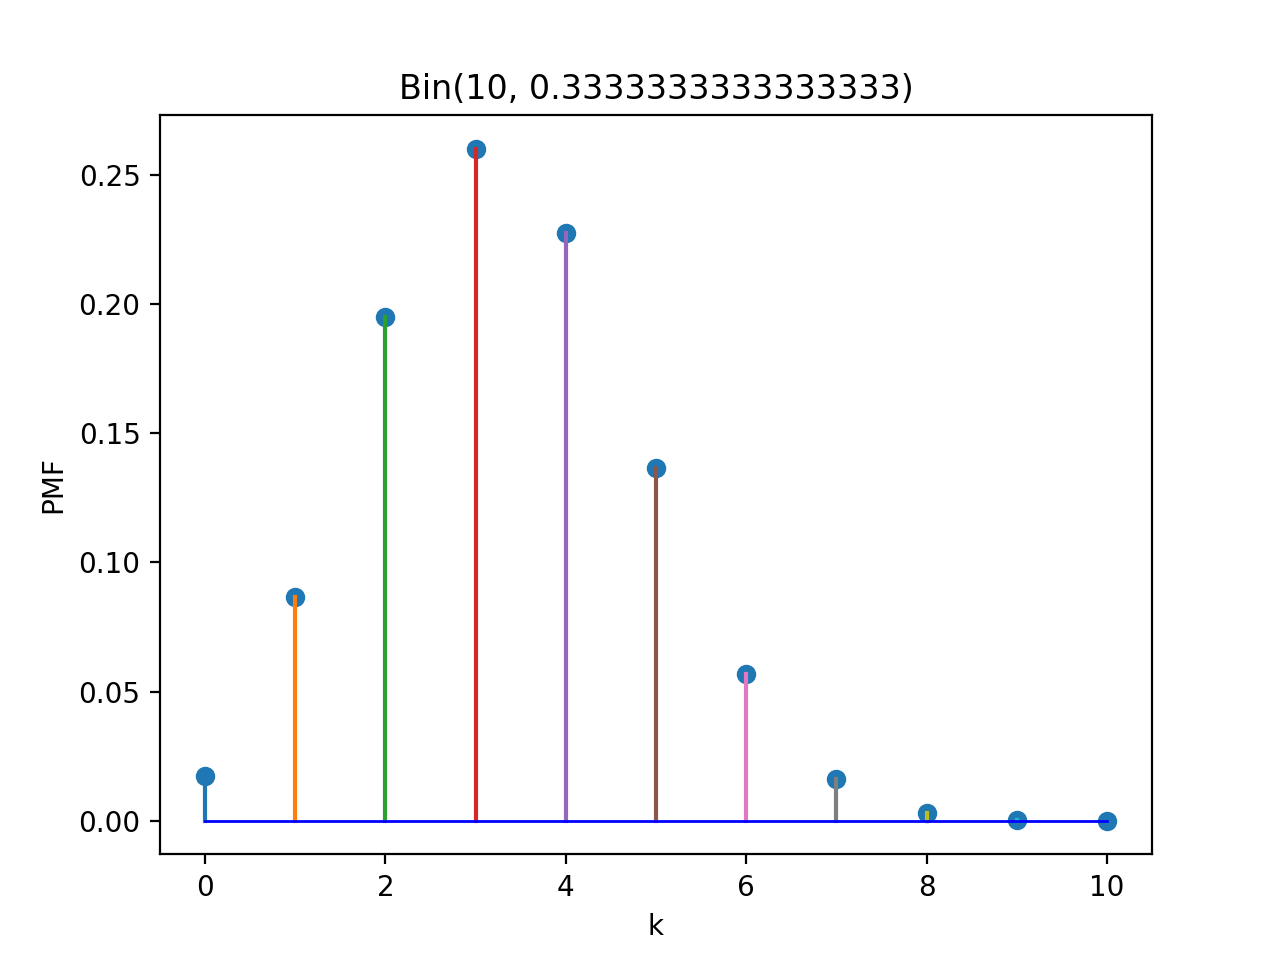
\epsfig{file=Abbildungen/bin10third.png, scale=0.45}
   \caption{Die Binomial-Verteilungen $\mathrm{Bin}(10,1/2)$ und $\mathrm{Bin}(10,1/3)$.}
  \label{fig:bin10.png}
\end{figure}

\begin{figure}[!ht]
  \centering
   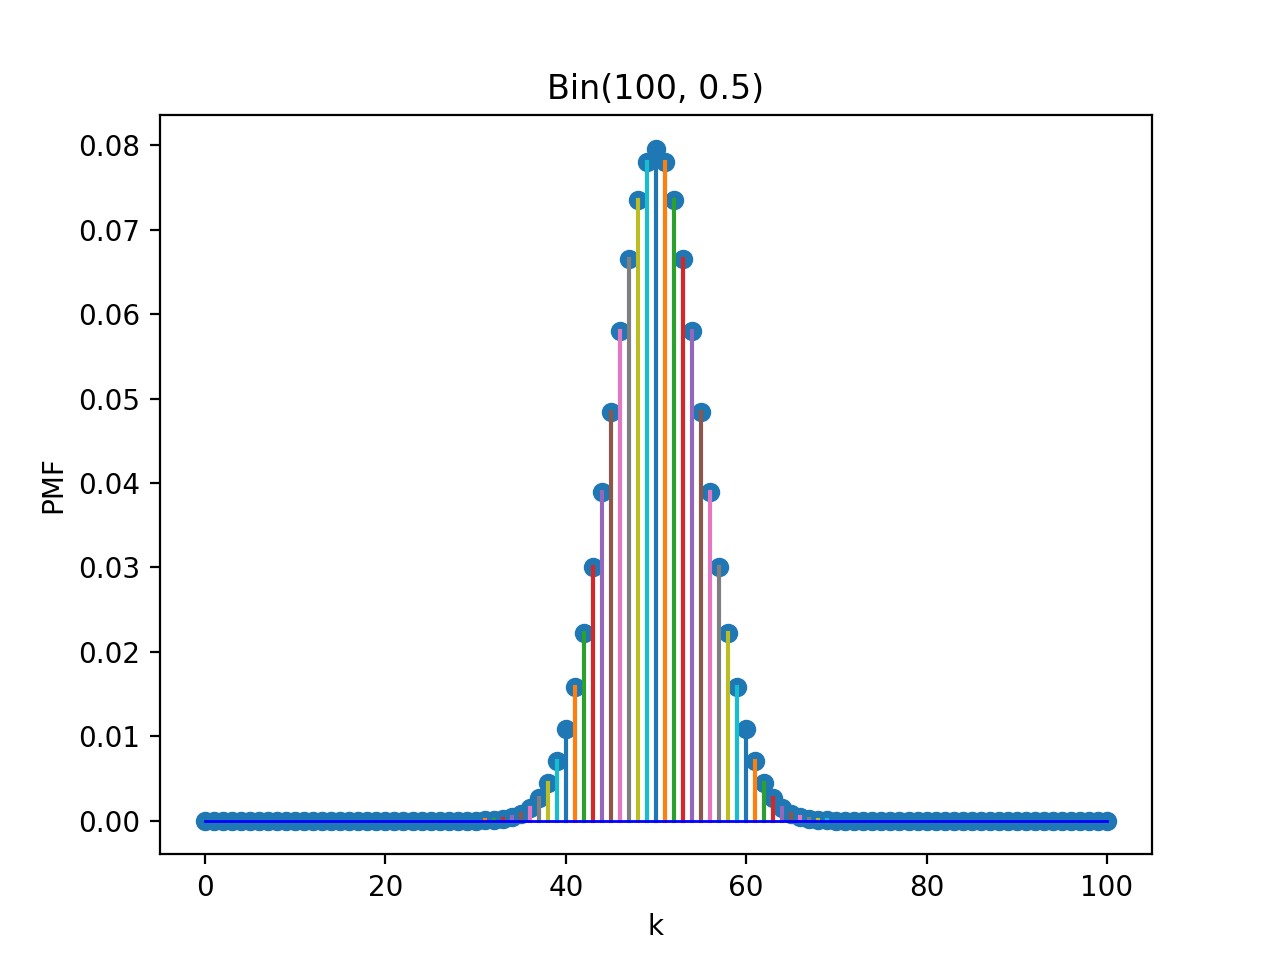
\epsfig{file=Abbildungen/bin100half.png, scale=0.45}
   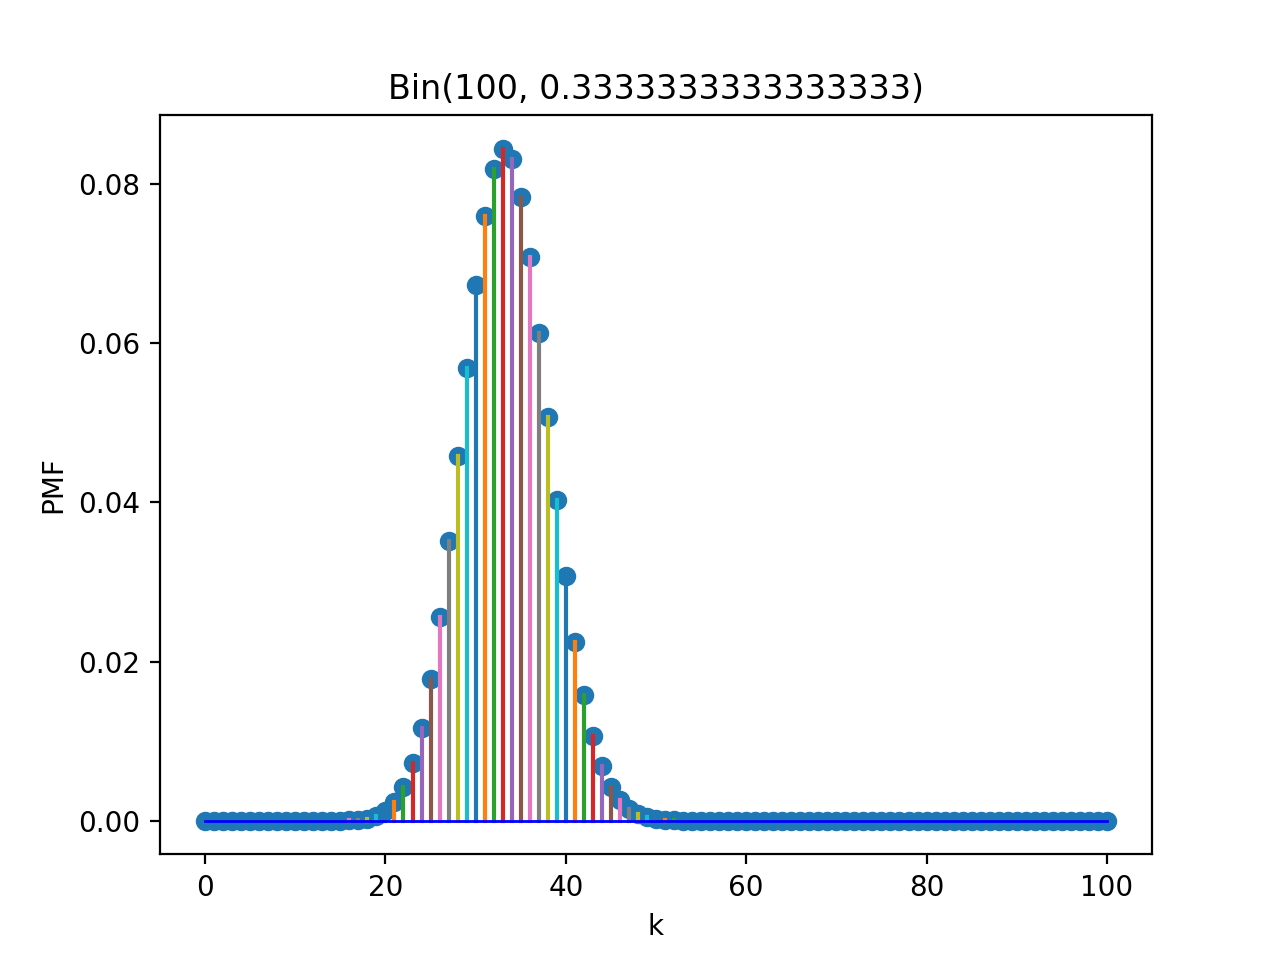
\epsfig{file=Abbildungen/bin100third.png, scale=0.45}
   \caption{Die Binomial-Verteilungen $\mathrm{Bin}(100,1/2)$ und $\mathrm{Bin}(100,1/3)$.}
  \label{fig:bin100.png}
\end{figure}



\section{Erwartungswert und Varianz}
\begin{Definition}[Erwartungswert]
  Ist $\langle \Omega, 2^\Omega, P \rangle$ ein diskreter Wahrscheinlichkeits-Raum und ist 
  \\[0.2cm]
  \hspace*{1.3cm}
  $X: \Omega \rightarrow \mathbb{R}$
  \\[0.2cm]
  eine Zufalls-Variable, so definieren wir den \blue{Erwartungswert} $E[X]$ als 
  \\[0.2cm]
  \hspace*{1.3cm}
  $\ds E[X] := \sum\limits_{\omega\in\Omega} P(\{\omega\}) \cdot X(\omega)$.
  \\[0.2cm]
  Hat der  Wertebereich von $X$ die Form 
  \\[0.2cm]
  \hspace*{1.3cm}
  $X(\Omega) = \{ X(\omega) \;|\; \omega\in \Omega \} = \{ x_n \;|\; n\in\mathbb{N} \}$, 
  \\[0.2cm]
  so k�nnen wir den Erwartungswert auch durch die Formel 
  \\[0.2cm]
  \hspace*{1.3cm}
  $\ds E[X] = \sum\limits_{n=0}^\infty P(X = x_n) \cdot x_n$
  \\[0.2cm]
  berechnen.  Eine analoge Formel gilt, wenn die Menge $X(\Omega)$ endlich ist. \qed
\end{Definition}

Der Erwartungswert einer Zufalls-Variable gibt den durchschnittlichen Wert an, der sich bei
einer gro�en Zahl von Versuchen ergeben w�rde.  Diese Aussage werden wir sp�ter noch n�her
pr�zisieren und dann auch beweisen k�nnen.

\example
Wir berechnen den Erwartungswert der Augenzahl beim W�rfeln mit einem W�rfel. 
Es gilt \\
\hspace*{1.3cm}
$
\begin{array}[t]{lcl}
 E[S] & = & \ds \sum\limits_{s=1}^6 P(S=s) \cdot s \\[0.5cm]
      & = & \ds \sum\limits_{s=1}^6 \frac{1}{6} \cdot s \;=\; \frac{1}{6} \cdot \sum\limits_{s=1}^6 s \\[0.5cm]
      & = & \ds \frac{1}{6} \cdot \frac{1}{2} \cdot 6 \cdot (6+1) \;=\; \frac{7}{2} \\[0.3cm]
\end{array}
$
\\[0.2cm]
Als n�chstes berechnen wir den Erwartungswert der Augensumme f�r das
W�rfeln mit zwei Laplace-W�rfeln.  Hier gilt
\\[0.2cm]
\hspace*{1.3cm}
$
\begin{array}[t]{lcl}
  
 E[S] & = & \ds \sum\limits_{s=2}^{12} P(S=s)\cdot s \\[0.5cm]
      & = & \ds \frac{1}{36} \cdot \sum\limits_{s=2}^7 (s-1)\cdot s +
                \frac{1}{36} \cdot \sum\limits_{s=8}^{12} (13-s)\cdot s \\[0.5cm]
      & = & \ds \frac{252}{36} \;=\; 7 
\end{array}
$
\\[0.2cm]
Dieses Ergebnis war auch zu erwarten, denn beim W�rfeln mit einem W�rfel ist der Erwartungswert
$\frac{7}{2}$ und der Erwartungswert der Augensumme beim W�rfeln mit zwei
W�rfeln sollte doppelt so gro� sein. \eox

\exercise 
Beim \blue{Mensch-�rger-dich-nicht} m�ssen Sie am Anfang eine 6 w�rfeln um das Spiel
beginnen zu k�nnen.  Berechnen Sie den Erwartungswert f�r die Anzahl der W�rfe, die
ben�tigt werden um eine 6 zu w�rfeln.

\solution Die Wahrscheinlichkeit, dass die 6 sofort beim ersten Wurf kommt, betr�gt
$\frac{1}{6}$, w�hrend die Wahrscheinlichkeit, dass beim ersten Wurf keine 6 gew�rfelt
wird, offenbar den Wert $\frac{5}{6}$ hat.  Die Wahrscheinlichkeit daf�r, dass im zweiten
Wurf die 6 f�llt, ist das Produkt aus der Wahrscheinlichkeit, dass im ersten Wurf keine 6
f�llt und der Wahrscheinlichkeit, dass im zweiten Wurf eine sechs f�llt und hat daher den
Wert $\frac{5}{6} \cdot \frac{1}{6}$.  Allgemein hat die Wahrscheinlichkeit daf�r, dass erst im
$n+1$-ten Wurf eine 6 f�llt, den Wert
\\[0.2cm]
\hspace*{1.3cm} $\ds \left(\frac{5}{6}\right)^n \cdot \frac{1}{6}$.
\\[0.2cm]
Bezeichnen wir die Zufalls-Variable, welche die Anzahl der ben�tigten W�rfe angibt, mit $N$, so
erhalten wir f�r den Erwartungswert von $N$ die Formel 
\\[0.2cm]
\hspace*{1.3cm}
$\ds E[N] = \sum\limits_{n=0}^\infty \left(\frac{5}{6}\right)^n \cdot\frac{1}{6} \cdot (n+1) = 
\frac{1}{6} \cdot \sum\limits_{n=0}^\infty \left(\frac{5}{6}\right)^n \cdot (n+1)$.
\\[0.2cm]
Diese Summe k�nnen wir mit einem Trick auf die \blue{geometrische Reihe} zur�ck f�hren.
Wir haben im letzten Semester gesehen, dass f�r alle $q \in ]-1,1[$ 
\\[0.2cm]
\hspace*{1.3cm}
$\ds \sum\limits_{n=0}^\infty q^n = \frac{1}{1-q}$
\\[0.2cm]
gilt.  Differenzieren wir diese Formel nach $q$, so erhalten wir die Gleichung
\\[0.2cm]
\hspace*{1.3cm}
$\ds \sum\limits_{n=1}^\infty n\cdot q^{n-1} = \frac{1}{(1-q)^2}$.
\\[0.2cm]
Die Summe auf der linken Seite geht erst bei $n=1$ los, denn das konstante Glied f�llt
beim Differenzieren weg.  Ersetzen wir in dieser Summe $n$ durch $n+1$, so haben wir 
\\[0.2cm]
\hspace*{1.3cm}
$\ds \sum\limits_{n=0}^\infty (n+1)\cdot q^{n} = \frac{1}{(1-q)^2}$.
\\[0.2cm]
Diese Summe hat aber  genau die Form, die oben bei der Berechnung des Erwartungswerts
auftritt.  Damit gilt 
\\[0.2cm]
\hspace*{1.3cm}
$\ds E[N] 
 = \frac{1}{6} \cdot \sum\limits_{n=0}^\infty \left(\frac{5}{6}\right)^n \cdot (n+1)
 = \frac{1}{6} \cdot \frac{1}{\bigl(1-\frac{5}{6}\bigr)^2} 
 = \frac{1}{6} \cdot \frac{1}{\bigl(\frac{1}{6}\bigr)^2} = 6$.
\\[0.2cm]
Wir m�ssen im Schnitt also 6 mal w�rfeln bis eine 6 auftritt.  Dieses Ergebnis ist intuitiv einleuchtend.
\eox 

Der Erwartungswert gibt den mittleren Wert einer Zufalls-Variable wieder. 
Damit wissen wir aber noch nichts dar�ber, wie weit die einzelnen Werte der Zufalls-Variable
um diesen Mittelwert streuen.  Dar�ber gibt die \blue{Varianz} Aufschluss.

\begin{Definition}[Varianz, Standard-Abweichung] \hspace*{\fill} \\
  Ist $\langle \Omega, 2^\Omega, P \rangle$ ein Wahrscheinlichkeits-Raum und ist 
  \\[0.2cm]
  \hspace*{1.3cm}
  $X: \Omega \rightarrow \mathbb{R}$
  \\[0.2cm]
  eine Zufalls-Variable, so definieren wir die \blue{Varianz} $\mathrm{Var}[X]$ als 
  den Erwartungswert der Zufalls-Variable $\omega \mapsto \bigr(X(\omega) - E[X]\bigr)^2$, also gilt
  \\[0.2cm]
  \hspace*{1.3cm}
  $\ds \mathrm{Var}[X] := E\bigl[(X - E[X])^2\bigr]$.
  \\[0.2cm]
  Hat der  Wertebereich von $X$ die Form 
  \\[0.2cm]
  \hspace*{1.3cm}
  $X(\Omega) = \{ X(\omega) \;|\; \omega\in \Omega \} = \{ x_n \;|\; n\in\mathbb{N} \}$
  \\[0.2cm]
  und setzen wir zur Abk�rzung $\mu = E[X]$,
  so k�nnen wir die Varianz auch durch die Formel 
  \\[0.2cm]
  \hspace*{1.3cm}
  $\ds \mathrm{Var}[X] = \sum\limits_{n=0}^\infty P(X = x_n) \cdot (x_n - \mu)^2$
  \\[0.2cm]
  berechnen.  Eine analoge Formel gilt, wenn die Menge $X(\Omega)$ endlich ist. 

  Die \blue{Standard-Abweichung} ist als die Quadrat-Wurzel aus der Varianz definiert
  \\[0.2cm]
  \hspace*{1.3cm}
  $\sigma(X) := \sqrt{\mathrm{Var}[X]\,}$.
  \\[0.2cm]
  Im Gegensatz zur Varianz hat die Standard-Abweichung dieselbe Einheit wie die Zufalls-Variable $X$.
  \eox
\end{Definition}

\example
Wir berechnen die Varianz der Zufalls-Variable $S$, welche die {Augenzahl} beim
W�rfeln mit einem W�rfel wiedergibt.  Wegen $E[S] = \frac{7}{2}$  gilt \\
\hspace*{1.3cm}
$
\begin{array}[t]{lcl}
 \mathrm{Var}[S] & = & \ds \sum\limits_{s=1}^6 P(S=s) \cdot \left(s - \frac{7}{2}\right)^2 \\[0.5cm]
      & = & \ds \sum\limits_{s=1}^6 \frac{1}{6} \cdot \left(s - \frac{7}{2}\right)^2 
      \;=\; \ds \frac{1}{6} \cdot \sum\limits_{s=1}^6 \left(s - \frac{7}{2}\right)^2 \\[0.5cm]
      & = & \ds \frac{35}{12}.
\end{array}
$
\\[0.2cm]
Damit gilt f�r die Standard-Abweichung 
\\[0.2cm]
\hspace*{1.3cm}
$\ds \sigma(X) = \sqrt{\frac{35}{12}\,} \approx 1.707825129$. 
\\[0.2cm]
F�hren wir dieselbe Rechnung f�r das Experiment ``W�rfeln mit  zwei W�rfeln'' durch, so
erhalten wir f�r die Varianz
\\[0.2cm]
\hspace*{1.3cm}
$
\begin{array}[t]{lcl}
  
 \textsl{Var}[S] & = & \ds \sum\limits_{s=2}^{12} P(S=s)\cdot (s - 7)^2 \\[0.5cm]
      & = & \ds \frac{1}{36} \cdot \sum\limits_{s=2}^7 (s-1)\cdot (s - 7)^2 +
                \frac{1}{36} \cdot \sum\limits_{s=8}^{12} (13-s)\cdot (s-7)^2 \\[0.5cm]
      & = & \ds \frac{35}{6}
\end{array}
$
\\[0.2cm]
Wir sehen, dass die Varianz jetzt genau doppelt so gro� ist wie beim W�rfeln mit einem W�rfel.
Diese Beobachtung werden wir sp�ter verallgemeinern und beweisen.
\qed


%%% Local Variables: 
%%% mode: latex
%%% TeX-master: "statistik"
%%% ispell-local-dictionary: "deutsch8"
%%% End: 

\chapter[Berechnung der Binomial-Koeffizienten]{Praktische Berechnung von Fakult�t und \\ Binomial-Koeffizienten}
In der Wahrscheinlichkeits-Rechnung verfolgen uns die Fakult�t und die 
Binomial-Koeffizienten auf Schritt und Tritt.  F�r kleine Werte von $n$ k�nnen wir $n!$
und ${n \choose k}$ problemlos mit dem Taschenrechner ausrechnen.  Aber schon bei der
L�sung von Aufgabe 5 st��t der Taschenrechner an seine Grenzen, denn der Ausdruck 
\\[0.1cm]
\hspace*{1.3cm}
$\ds {40\,000 \choose 200}$,
\\[0.1cm]
der bei der L�sung dieser Aufgabe im Nenner auftritt, liefert eine ganze Zahl mit 545
Stellen.  Zwar kann \textsc{SetlX} solche Zahlen noch m�helos berechnen, aber in vielen andern
Programmier-Sprachen k�nnen Sie mit solchen Zahlen nicht mehr arbeiten.   Wir stellen daher in diesem Abschnitt
eine N�herungs-Formel f�r die Fakult�t und f�r den Binomial-Koeffizienten vor. 
Wir beginnen mit einer Approximation der Fakult�t.
Die klassische \href{https://de.wikipedia.org/wiki/Stirlingformel}{N�herung von Stirling} 
(\href{https://de.wikipedia.org/wiki/James_Stirling_(Mathematiker)}{James Stirling}; 1692 - 1770) lautet  
\\[0.1cm]
\hspace*{1.3cm}
$\ds n! \approx \sqrt{2 \cdot \pi \cdot n\,} \cdot \left(\frac{n}{\mathrm{e}}\right)^n$.
\\[0.1cm]
Hier bezeichnet $\mathrm{e}$ die \href{https://de.wikipedia.org/wiki/Eulersche_Zahl}{Eulersche Zahl}.
Genauer ist die Formel des ungarischen Mathematikers 
\href{https://en.wikipedia.org/wiki/Cornelius_Lanczos}{Cornelius Lanzcos} (1893 - 1974). 
Diese Formel lautet:  
\\[0.1cm]
\hspace*{1.3cm}
$\ds n! \approx \sqrt{2 \cdot \pi\;} \cdot \left(\frac{n+ \frac{1}{2}}{\mathrm{e}}\right)^{n+\frac{1}{2}}$.
\\[0.1cm]
Die Formel auf der rechten Seite approximiert die Fakult�t in dem folgenden Sinne: Es gilt
\\[0.3cm]
\hspace*{1.3cm}
$\ds \lim\limits_{n\rightarrow \infty} \frac{\sqrt{2 \cdot \pi\;} \cdot
  \left(\frac{n+ \frac{1}{2}}{e}\right)^{n+\frac{1}{2}}}{n!} = 1$.
\\[0.3cm]
F�r eine Herleitung dieser Formeln bleibt uns leider nicht die Zeit.  Oft sind die
Fakult�ten so gro�, dass Sie nicht mehr auf dem Taschenrechner dargestellt werden k�nnen.
Sie treten dann meist in Br�chen auf und der zu berechnende Bruch ist durchaus noch
darstellbar. Dann kann es hilfreich sein, zum Logarithmus �berzugehen.   Um beispielsweise
${n \choose k}$ zu berechnen, gehen wir wie folgt vor: 
\begin{equation}
  \label{eq:binappr}  
\begin{array}[b]{lcl}
\ds 
 {n \choose k} & = & \ds \frac{n!}{k! \cdot (n-k)!} \\[0.3cm]
                & = & \ds \exp\left(\ln\left(\frac{n!}{k! \cdot (n-k)!}\right)\right) \\[0.3cm]  
                & = & \ds \exp\Bigl(\ln\bigl(n!\bigr) - \ln\bigl(k!\bigr) - \ln\bigl((n-k)!\bigr)\Bigr) \\[0.3cm]  
\end{array}
\end{equation}
Zu Berechnung der verschiedenen Fakult�ten in dieser Formel wenden wir auf die N�herungsformel von Lanzcos den
Logarithmus an und erhalten 
\\[0.1cm]
\hspace*{1.3cm}
$\ds \ln\bigl(n!\bigr) \approx  \frac{1}{2}\cdot\ln(2\cdot \pi) + \left(n+\frac{1}{2}\right) \cdot \left( \ln\Bigl(n + \frac{1}{2}\Bigr) - 1 \right)$.
\\[0.1cm]
Setzen wir diesen Wert in Gleichung (\ref{eq:binappr}) ein, so  k�nnen wir den
Binomial-Koeffizienten approximieren.
Berechnen wir ${100 \choose 50}$ auf diese Weise, so erhalten wir 
\\[0.1cm]
\hspace*{1.3cm}
$\ds {100 \choose 50} \approx 1.007667751 \cdot 10^{29}$.
\\[0.1cm]
Der exakte Wert ist
\\[0.1cm]
\hspace*{1.3cm}
$\ds {100 \choose 50} = 100\,891\,344\,545\,564\,193\,334\,812\,497\,256$
\\[0.1cm]
und der relative Fehler liegt bei $1.2$\textperthousand.  Bei der Berechnung von
Wahrscheinlichkeiten sind solche Genauigkeiten meistens ausreichend.

Noch einfacher k�nnen Binomial-Koeffizienten �ber die Formel 
\\[0.3cm]
\hspace*{1.3cm}
$\ds
 {n \choose k} \approx \sqrt{\frac{2}{\pi \cdot n}} \cdot 2^n \cdot \exp\left(-\frac{\bigl(k - \frac{1}{2}\cdot
     n\bigr)^2}{\frac{1}{2}\cdot n}\right)$.
\\[0.3cm]
berechnet werden.  Diese Formel geht auf 
\href{https://en.wikipedia.org/wiki/Abraham_de_Moivre}{Abraham de Moivre} (1667 - 1754) 
zur�ck.  Diese N�herung liefert brauchbare Werte sobald die
Bedingung $n > 36$ erf�llt ist.  Die Werte sind am genauesten f�r $k \approx \frac{n}{2}$.
Berechnen wir mit dieser Formel eine N�herung f�r ${100 \choose 50}$, so erhalten wir 
\\[0.1cm]
\hspace*{1.3cm}
$\ds {100 \choose 50} \approx 1.0114388424145895 \cdot 10^{29}$.
\\[0.1cm]
Diesmal liegt der relative Fehler bei $2.5$\textperthousand\ und ist damit doppelt so hoch
wie bei der Verwendung der Formel von Lanzcos.

Der Binomial-Koeffizient tritt oft in Termen der Form 
\\[0.1cm]
\hspace*{1.3cm}
$\ds {n \choose k} \cdot p^k \cdot (1-p)^{n-k}$ 
\\[0.1cm]
auf.  
F�r diesen Fall gibt es noch eine Approximations-Formel, die einfacher zu handhaben
ist.  Die Formel lautet 
\\[0.1cm]
\hspace*{1.3cm}
$\ds {n \choose k} \cdot p^k \cdot (1-p)^{n-k} 
  \approx \frac{1}{\sqrt{2\cdot \pi \cdot n \cdot p \cdot (1-p)\;}} \cdot 
          \exp\left(-\frac{(k - n \cdot p)^2}{2 \cdot n \cdot p \cdot (1 - p)}\right)$
\\[0.1cm]
und geht auf \href{https://en.wikipedia.org/wiki/Pierre-Simon_Laplace}{Pierre Simon Laplace} (1749 - 1827)
zur�ck.  Diese N�herung liefert brauchbare Werte sobald die Bedingung
\\[0.1cm]
\hspace*{1.3cm}
$n \cdot p \cdot (1 - p) > 9$
\\[0.1cm]
erf�llt ist.  F�r $p= \frac{1}{2}$ geht diese Formel in die von de Moivre angegebene
Formel �ber.  Die Werte, die mit dieser Formel berechnet werden, sind am brauchbarsten f�r
die Werte von $k$, die in der N�he von $n \cdot p$ liegen.

Normalerweise interessiert uns nicht eine einzelne Wahrscheinlichkeit der Form 
\\[0.1cm]
\hspace*{1.3cm}
$\ds {n \choose k} \cdot p^k \cdot (1 - p)^{n-k}$,
\\[0.1cm]
sondern wir wollen vielmehr wissen, welchen Wert ein Ausdruck der Form 
\\[0.1cm]
\hspace*{1.3cm}
$\ds \sum\limits_{i=0}^k {n \choose i} \cdot p^i \cdot (1 - p)^{n-i}$
\\[0.1cm]
annimmt, denn dieser Ausdruck gibt die Wahrscheinlichkeit daf�r an, dass bei einer
Binomial-Verteilung bei einer $n$-fachen Durchf�hrung eines Experiments 
ein Ergeignis h�chstens $k$-mal auftritt.  Wir wollen daher jetzt eine N�herung f�r diese
Summe herleiten.  Dazu definieren wir zun�chst 
\\[0.1cm]
\hspace*{1.3cm}
$\ds F^n_p(k) := \sum\limits_{i=0}^k {n \choose i} \cdot p^i \cdot (1 - p)^{n-i}$.
\\[0.1cm]
Die Funktion $F^n_p(k)$ bezeichnen wir auch als die \blue{Verteilungsfunktion}.
Um die nachfolgende Rechnung zu vereinfachen, definieren wir zur Abk�rzung 
\\[0.1cm]
\hspace*{1.3cm}
$\mu := n \cdot p$, \quad $q := 1 - p$ \quad und \quad $\sigma := \sqrt{n \cdot p \cdot q\,}$.
\\[0.1cm]
Allgemein l�sst sich eine Summe der Form $\sum_{i=0}^k f(i)$ wie folgt durch ein Integral
approximieren: 
\\[0.1cm]
\hspace*{1.3cm}
$\ds \sum\limits_{i=a}^b f(i) \approx \int_{a-\frac{1}{2}}^{b+\frac{1}{2}} f(t)\dx t$
\\[0.1cm]
Wir approximieren nun in der Definition der Verteilungsfunktion $F^n_p(k)$ einerseits den
Binomial-Koeffizienten durch die Formel von Laplace und andererseits n�hern wir die Summe
durch ein Integral an.  Dann erhalten wir 
\\[0.1cm]
\hspace*{1.3cm}
$
\begin{array}[t]{lcl}
 F^n_p(k) & =       & \ds 
                      \sum\limits_{i=0}^k {n \choose i} \cdot p^i \cdot (1 - p)^i \\[0.5cm]
          & \approx & \ds 
                      \sum\limits_{i=0}^k \frac{1}{\sqrt{2 \, \pi \,n \, p \, (1-p)\;}} \cdot \exp\left(-\frac{(i - n \cdot p)^2}{2 \, n \, p \,(1 - p)}\right) \\[0.5cm]
          & =       & \ds
                      \sum\limits_{i=0}^k \frac{1}{\sqrt{2\, \pi\;} \cdot \sigma} \cdot \exp\left(-\frac{(i - \mu)^2}{2\, \sigma^2}\right) \\[0.5cm]
          & \approx & \ds
                      \int_{-\frac{1}{2}}^{k+\frac{1}{2}} \frac{1}{\sqrt{2\, \pi\;} \cdot \sigma} \cdot \exp\left(-\frac{(u - \mu)^2}{2\, \sigma^2}\right)\dx u \\[0.5cm]
          & =       & \ds
                      \frac{1}{\sqrt{2\, \pi\;} \cdot \sigma} \cdot \int_{-\frac{1}{2}}^{k+\frac{1}{2}} \exp\left(-\frac{(u - \mu)^2}{2\, \sigma^2}\right)\dx u \\[0.5cm]
\end{array}
$
\\[0.1cm]
Das hier auftretende Integral vereinfachen wir, indem wir die Variablen-Substitution 
\\[0.1cm]
\hspace*{1.3cm}
$\ds t(u) = \frac{u - \mu}{\sigma}$, \quad also $\dx t = \frac{1}{\sigma} \dx u$\quad $\sigma\dx t = \dx u$
\\[0.1cm]
durchf�hren.  Setzen wir hier f�r $u$ die Grenzen $-\frac{1}{2}$ bzw. $k+\frac{1}{2}$ ein,
so erhalten wir 
\\[0.1cm]
\hspace*{1.3cm}
$
\begin{array}[t]{lcl}
 F^n_p(k) & = & \ds \frac{1}{\sqrt{2\, \pi\;} \cdot \sigma} \cdot 
                \int\limits_{(-\frac{1}{2}-\mu)/\sigma}^{(k+\frac{1}{2}-\mu)/\sigma} \exp\left(-\frac{t^2}{2}\right)\,\sigma\dx t \\[0.75cm]
 
          & = & \ds \frac{1}{\sqrt{2\, \pi\;}} \cdot 
                \int\limits_{(-\frac{1}{2}-\mu)/\sigma}^{(k+\frac{1}{2}-\mu)/\sigma} \exp\left(-\frac{t^2}{2}\right)\dx t 
\end{array}
$
\\[0.1cm]
Um an dieser Stelle weiter zu kommen, ben�tigen wir die Gau�'sche Integralfunktion
$\Phi(x)$.  Diese Funktion wird wie folgt definiert: 
\\[0.1cm]
\hspace*{1.3cm}
$\ds \Phi(x) = \frac{1}{\sqrt{2\,\pi}} \cdot \int_{-\infty}^x \exp\left(-\frac{t^2}{2}\right)\dx t$
\\[0.1cm]
Damit haben f�r die Verteilungsfunktion $F^n_p(k)$ die N�herung
\\[0.1cm]
\hspace*{1.3cm}
$\ds  F^n_p(k) = \Phi\Biggl(\frac{k+\frac{1}{2}-\mu}{\sigma}\Biggr) -   \Phi\Biggl(\frac{-\frac{1}{2}-\mu}{\sigma}\Biggr)$
\\[0.1cm]
gefunden.  Ber�cksichtigen wir noch, dass $\mu = n \cdot p$ und $\sigma = \sqrt{n\,p\,q}$ gilt und
bedenken, dass wir eine N�herung f�r gro�e Werte von $n$ suchen, so gilt 
\\[0.1cm]
\hspace*{1.3cm}
$\ds \Phi\left(\frac{-\frac{1}{2}-\mu}{\sigma}\right) =
  \Phi\left(\frac{-\frac{1}{2}-n\,p}{\sqrt{n\,p\,q}}\right) 
  \stackrel{\ds\longrightarrow}{_{n \rightarrow \infty}} \Phi\left(-\infty\right) = 0$
\\[0.1cm]
Damit lautet unsere N�herung f�r die Verteilungsfunktion $F^n_p(k)$ 
\\[0.1cm]
\hspace*{1.3cm}
$\ds F^n_p(k) \approx \Phi\Biggl(\frac{k+\frac{1}{2}- n\,p}{\sqrt{n\,p\,q\,}}\Biggr)$.
\\[0.1cm]
In dieser Formel wird h�ufig die sogenannte \emph{Stetigkeits-Korrektur} $\frac{1}{2}$
weggelassen, denn gegen�ber dem Term $n\,p$ f�llt diese kaum ins Gewicht.
Wir werden also im folgenden die N�herung
\\[0.3cm]
\hspace*{1.3cm}
\framebox{$\ds F^n_p(k) \approx \Phi\Biggl(\frac{k- n\,p}{\sqrt{n\,p\,q\,}}\Biggr)$}
\\[0.3cm]
verwenden.  Die $\Phi$-Funktion ist in \textsc{SetlX} vordefiniert und hat dort den Namen
\texttt{stat\_normalCDF}.  Diese Funktion wird mit drei Parametern aufgerufen.  Es gilt
\\[0.2cm]
\hspace*{1.3cm}
$\Phi(x) = \mathtt{stat\_normalCDF}(x, 0, 1)$.
\\[0.2cm]
Damit sind wir jetzt in der Lage, auch interessantere Aufgaben aus der
Wahrscheinlichkeits-Rechnung numerisch zu l�sen. 

\exercise
Angenommen, wir w�rfeln $n$ mal mit einem Laplace-W�rfel.  Wie gross muss $n$ gew�hlt
werden, damit wir mit einer  Wahrscheinlichkeit von $99\%$ davon ausgehen k�nnen, 
dass mindestens $\frac{n}{7}$ mal eine Sechs  gew�rfelt wird?

%%% Local Variables: 
%%% mode: latex
%%% TeX-master: "statistik"
%%% ispell-local-dictionary: "deutsch8"
%%% End: 

\chapter{Bedingte Wahrscheinlichkeiten}
In diesem Abschnitt beantworten wir die folgende Frage: Es sei ein
Wahrscheinlichkeits-Raum $\langle \Omega, 2^\Omega, P \rangle$ gegeben.  Wir
betrachten ein Ereignis $A\in 2^\Omega$.  Angenommen wir erfahren nun, dass ein
Ereignis $B$ eingetreten ist.  Wie ver�ndert sich durch diese Information die
Wahrscheinlichkeit f�r das Eintreten des Ereignisses $A$?  Die 
Wahrscheinlichkeit f�r das Eintreten von $A$ unter der Voraussetzung, dass $B$
bereits eingetreten ist, bezeichnen wir mit
\\[0.2cm]
\hspace*{1.3cm} $P(A|B)$.

\example Wir betrachten das Zufalls-Experiment ``\blue{Wurf eines
  Laplace-W�rfels}'' mit dem Ergebnis-Raum $\Omega = \{1,\cdots,6\}$.  Es sei $A$
das Ereignis, dass eine 6 gew�rfelt wird, also $A = \{6\}$.  Da wir
vorausgesetzt haben, dass es sich um einen Laplace-W�rfel handelt, gilt 
\\[0.2cm]
\hspace*{1.3cm} $\ds P(A) = \frac{1}{6}$.
\\[0.2cm]
Es sei weiterhin $B$ das Ereignis, dass die Augenzahl gr��er als 4 ist, also
$B = \{5,6\}$.  Wir nehmen nun an, dass der W�rfel geworfen wird und wir gesagt
bekommen, dass das Ereignis $B$ eingetreten ist.  Das genaue Ergebnis des
Zufalls-Experiments ist uns allerdings nicht bekannt.  Da dann nur noch zwei M�glichkeiten f�r das Ergebnis 
bleiben, n�mlich die Zahlen 5 und 6, w�rden wir in dieser neuen Situation dem
Ereignis $A$ die Wahrscheinlichkeit $\frac{1}{2}$ zuordnen, also gilt 
\\[0.2cm]
\hspace*{1.3cm}
$\ds P(A|B) = \frac{1}{2}$. \eox


\example
Aus einer Sterbetafel, in der das Lebensalter von $100\,000$ Frauen
verzeichnet ist,  entnehmen wir die Information, dass $89\,835$
aller Frauen das Alter von mindestens 60 Jahren erreichen, w�hrend $57\,062$ ein
Alter von mehr als 80 Jahren erreichen.  Angenommen, eine Frau wird 60 Jahre alt.
Mit welcher Wahrscheinlichkeit erreicht Sie dann ein Alter von 80 Jahren?

Wir bezeichnen das Ereignis, dass eine Frau das Alter von $60$ Jahren erreicht, mit
$A$, w�hrend das Ereignis, dass eine Frau das Alter von $80$ Jahren erreicht, mit 
$B$ bezeichnet wird.  Offenbar ist $B$ eine Teilmenge von $A$ und es ist klar, dass
der Anteil der sechzigj�hrigen Frauen, die auch noch das Alter von 80 Jahren
erreichen, durch den Bruch $\frac{|B|}{|A|}$ gegeben wird.  Also gilt 
\\[0.2cm]
\hspace*{1.3cm}
$\ds P(B|A) = \frac{|B|}{|A|} = \frac{57\,062}{89\,835} \approx 0.63519$. 
\\[0.2cm]
Damit betr�gt also die Wahrscheinlichkeit daf�r, dass eine sechzigj�hrige Frau das
Alter von 80 Jahren erreicht, $63.5\%$.
\eox

\next Wir verallgemeinern die obigen Beispiele.  Wir gehen davon aus, dass ein
Wahrscheinlichkeits-Raum
\\
\hspace*{1.3cm} $\langle \Omega, 2^\Omega, P \rangle$
\\[0.2cm]
mit einer gleichm��igen Wahrscheinlichkeits-Verteilung $P$ gegeben ist, es gilt also
\\[0.2cm]
\hspace*{1.3cm} $\ds P(E) = \frac{|E|}{|\Omega|}$ \quad f�r alle $E \in
2^\Omega$.
\\[0.2cm]
Wir betrachten zwei Ereignisse $A$ und $B$ und berechnen die bedingte
Wahrscheinlichkeit f�r das Eintreten von $B$, wenn wir bereits wissen, dass $A$
eingetreten ist.  Wenn $A$ eingetreten ist, kommen f�r das Eintreten von $B$ nur
noch die Ergebnisse in Frage, die in $B \cap A$ liegen.  Nehmen wir an, dass diese
Ergebnisse nach wie vor dieselbe Wahrscheinlichkeit haben, dann haben wir einen
neuen Wahrscheinlichkeits-Raum, dessen Ereignis-Raum die Menge $A$ ist.  Folglich
gilt
\begin{equation}
  \label{eq:condProb}  
\ds P(B|A) = \frac{|B \cap A|}{|A|} 
   = \frac{\frac{|B \cap A|}{|\Omega|}}{\frac{|A|}{|\Omega|}}
   = \frac{P(B \cap A)}{P(A)}.
\end{equation}
Diese Gleichung f�r die bedingte Wahrscheinlichkeit gilt auch im allgemeinen Fall.
Sind zwei Ereignisse $A$ und $B$ gegeben und f�hren wir das zugrunde liegende
Zufalls-Experiment $n$-mal aus, so erwarten wir, dass f�r gro�e $n$ ein Ereignis
$E$ etwa $n \cdot P(E)$ mal eintritt.  Ist das Ereignis $A$ bereits eingetreten, so
tritt das Ereignis $B$ genau dann ein, wenn das Ereignis $B \cap A$ eintritt.  Also
ist die relative H�ufigkeit f�r das Eintreten des Ereignisses $B$ unter der Annahme,
dass $A$ bereits eingetreten ist, durch den Quotienten
\\[0.2cm]
\hspace*{1.3cm}
$\ds \frac{n \cdot P(B \cap A)}{n \cdot P(A)} = \frac{P(B \cap A)}{P(A)}$
\\[0.2cm]
gegeben und daher definieren wir die bedingte Wahrscheinlichkeit immer als diesen Quotienten.

\exercise
Eine Lieferung von Gl�hbirnen enthalte erfahrungsgem�� drei Arten von Gl�hbirnen:
\begin{enumerate}
\item Gl�hbirnen, die bereits defekt sind.  Der Anteil dieser Gl�hbirnen betrage
      $10\%$.
\item Gl�hbirnen, die zwar funktionieren, aber nur eine Lebensdauer von weniger als 10 Tagen haben.  Hier
      betr�gt der Anteil $20\%$. 
\item Gl�hbirnen, die voll funktionsf�hig sind.
\end{enumerate}
Angenommen, Sie testen eine Gl�hbirne und stellen fest, dass diese Birne noch nicht
defekt ist.  Wie hoch ist dann die Wahrscheinlichkeit daf�r, dass diese Gl�hbirne 
voll funktionsf�hig ist?

\solution
Wir bezeichnen das Ereignis ``\blue{Gl�hbirne defekt}'' mit $D$, das Ereignis
``\blue{Gl�hbirne hat kurze Lebensdauer}'' mit $K$ und das Ereignis
``\blue{Gl�hbirne voll funktionsf�hig}'' mit $F$.  Gefragt ist dann nach der
Wahrscheinlichkeit, dass die Gl�hbirne voll funktionsf�hig ist unter der Bedingung,
dass die Gl�hbirne nicht defekt ist.  Das ist genau die bedingte Wahrscheinlichkeit
$P(F|D^c)$:
\\[0.2cm]
\hspace*{1.3cm}
$
\begin{array}[t]{lcll}
 P(F|D^c) & = & \ds \frac{P(F \cap D^c)}{P(D^c)} \\[0.5cm]
          & = & \ds \frac{P\bigl(F \cap (K \cup F)\bigr)}{P(K \cup F)} 
              & \mbox{wegen $D^c = K \cup F$} \\[0.5cm]
          & = & \ds \frac{P\bigl((F \cap K) \cup (F \cap F)\bigr)}{P(K \cup F)} \\[0.5cm]
          & = & \ds \frac{P\bigl(\emptyset \cup F\bigr)}{P(K \cup F)} 
              & \mbox{wegen $F \cap K = \emptyset$} \\[0.5cm]
          & = & \ds \frac{P(F)}{P(K) + P(F)} 
              & \mbox{wegen $K \cap F = \emptyset$} \\[0.5cm]
          & = & \ds \frac{0.7}{0.2 + 0.7} 
              & \mbox{wegen $P(F) = 1 - P(D) - P(K)$} \\[0.5cm]
          & = & \ds \frac{7}{9}
\end{array}
$
\\[0.2cm]
Damit hat die gesuchte Wahrscheinlichkeit den Wert $0.\overline{7}$.

\next
Die Gleichung (\ref{eq:condProb}) zur Berechnung der bedingten Wahrscheinlichkeit
kann wie folgt umgestellt werden:
\begin{equation}
\label{eq:condProbCut}
P(B \cap A) = P(B|A) \cdot P(A)
\end{equation}

\exercise
Wir nehmen an, dass bei der Produktion von Gl�hbirnen die Wahrscheinlichkeit daf�r,
dass eine Gl�hbirne defekt ist, den Wert $0.1$ hat.  Diese Gl�hbirnen werden
anschlie�end in Kisten verpackt und ausgeliefert.  Die Wahrscheinlichkeit, dass eine
solche Kiste beim 
Transport hinf�llt, betrage $5\%$.  Au�erdem gehen wir davon aus, dass beim
Hinfallen einer Kiste $30\%$ der intakten Gl�hbirnen zerst�rt werden.
Berechnen Sie die Wahrscheinlichkeit daf�r, dass eine gelieferte Gl�hbirne
funktionsf�hig ist. 

\section{Die totale Wahrscheinlichkeit und die Formel von Bayes}
Es sei ein Wahrscheinlichkeits-Raum $\langle \Omega, 2^\Omega, P \rangle$ gegeben.
Wir betrachten zwei Ereignisse $A$ und $B$. Nach Definition des komplement�ren
Ereignisses gilt
\\[0.2cm]
\hspace*{1.3cm}
$B \cup B^c = \Omega$.
\\[0.2cm]
Wegen $A \cap \Omega = A$ folgt daraus 
\\[0.2cm]
\hspace*{1.3cm}
$A = A \cap (B \cup B^c) = (A \cap B) \cup (A \cap B^c)$.
\\[0.2cm]
Da die beiden Mengen $A \cap B$ und $A \cap B^c$ disjunkt sind, k�nnen wir damit die
Wahrscheinlichkeit des Ereignisses $A$ durch die folgende Formel berechnen:
\\[0.2cm]
\hspace*{1.3cm}
$
\begin{array}[t]{lcll}
P(A) & = & P(A \cap B) + P(A \cap B^c) \\[0.2cm]
     & = & P(A|B)\cdot P(B) + P(A|B^c)\cdot P(B^c) 
         & \mbox{nach Gleichung (\ref{eq:condProbCut})}
\end{array}
$
\\[0.2cm]
Dieses Ergebnis l�sst sich verallgemeinern.  Ist eine Familie $B_1$, $\cdots$, $B_n$
von Ereignissen gegeben, so dass 
\begin{enumerate}
\item $B_1 \cup \cdots \cup B_n = \Omega$ \quad und
\item $B_i \cap B_j = \emptyset$ f�r alle $i \not= j$
\end{enumerate}
gilt, so haben wir 
\begin{equation}
  \label{eq:condTotal}
\begin{array}[b]{lcl}
P(A) & = & P(A \cap B_1) + \cdots + P(A \cap B_n) \\[0.2cm]
     & = & P(A|B_1)\cdot P(B_1) + \cdots + P(A|B_n) \cdot P(B_n) \\[0.2cm]
     & = & \ds \sum\limits_{i=1}^n P(A|B_i)\cdot P(B_i).
\end{array}  
\end{equation}
Dies ist die Formel von der \blue{totalen Wahrscheinlichkeit}.
Eine Familie $B_1$, $\cdots$, $B_n$ von Ereignissen mit den oben angegebenen
Eigenschaften bezeichnen wir als \blue{Zerlegung} von $\Omega$.

\exercise
Erfahrungsgem�� sind etwa $8\%$ aller M�nner farbenblind, w�hrend nur $0.6\%$ aller
Frauen farbenblind sind.
Nehmen Sie an, dass der Anteil der M�nner in der Gesamtbev�lkerung $47\%$ betr�gt und
berechnen Sie die Wahrscheinlichkeit daf�r, dass eine beliebige Person farbenblind
ist.

\solution
Es sei $B$ das Ereignis, das eine Person farbenblind ist.  Das Ereignis, dass eine
Person m�nnlich ist bezeichnen wir mit $M$ und das dazu komplement�re Ereignis
bezeichnen wir mit $F$.  Dann gilt 
\\[0.2cm]
\hspace*{1.3cm}
$P(B) = P(B|M)\cdot P(M) + P(B|F) \cdot P(F) = 0.08 \cdot 0.47 + 0.006 \cdot 0.53 \approx 0.04078$.
\\[0.2cm]
Also sind etwa $4.1\%$ aller Personen farbenblind.
\eox

\next
Aus der Gleichung $P(B \cap A) = P(B|A) \cdot P(A)$ k�nnen wir eine weitere Formel ableiten:
\\[0.2cm]
\hspace*{1.3cm}
$
\begin{array}[t]{lcl}
  P(B|A) \cdot P(A) & = & P(B \cap A) \\[0.2cm]
                    & = & P(A \cap B) \\[0.2cm]
                    & = & P(A|B) \cdot P(B)
\end{array}
$
\\[0.2cm]
Teilen wir diese Formel durch $P(A)$, so ergibt sich 
\\[0.2cm]
\hspace*{1.3cm}
$\ds P(B|A) = \frac{P(A|B) \cdot P(B)}{P(A)}$
\\[0.2cm]
Nehmen wir nun an, dass $B_1$, $\cdots$, $B_n$ eine Zerlegung von $\Omega$ ist,
so gilt nach dem Satz von der totalen Wahrscheinlichkeit 
\\[0.2cm]
\hspace*{1.3cm}
$P(A) = \sum\limits_{i=1}^n P(A|B_i) \cdot P(B_i)$.
\\[0.2cm]
Gilt nun  $B = B_k$ f�r ein $k\in\{1,\cdots,n\}$, so haben wir insgesamt 
\begin{equation}
  \label{eq:bayes}
  \ds P(B_k|A) = \frac{P(A|B_k) \cdot P(B_k)}{\sum\limits_{i=1}^n P(A|B_i) \cdot P(B_i)}.
\end{equation}
Dies ist der \href{https://de.wikipedia.org/wiki/Satz_von_Bayes}{Satz von Bayes}
(\href{https://de.wikipedia.org/wiki/Thomas_Bayes}{Thomas Bayes, 1701 -- 1761}).  Diese Formel f�hrt
die Wahrscheinlichkeit daf�r, dass ein Ereignis $B_k$ unter der Bedingung
$A$ eintritt auf die Wahrscheinlichkeiten, dass das Ereignis $A$ unter der Bedingung
$B_i$ eintritt, zur�ck.  Die Formel von Bayes ist sehr wichtig im Bereich der Medizin
und der Rechtssprechung. Wir betrachten entsprechende Beispiele.

\example
Ein (hypothetischer) Bluttest erkennt das Vorliegen von Malaria mit einer
Wahrscheinlichkeit von $99.9\%$.  Mit einer Wahrscheinlichkeit von $0.5\permil$ liefert der Test aber 
auch dann ein positives Ergebnis, wenn keine Malaria vorliegt.
Die Wahrscheinlichkeit, dass eine Person aus Deutschland an Malaria erkrankt ist,
liegt bei etwa $10^{-6}$.  Angenommen, Sie machen diesen Bluttest und erhalten ein
positives Ergebnis.  Wie hoch ist dann die Wahrscheinlichkeit, dass Sie Malaria
haben?

\solution
Wir bezeichnen das Ereignis, dass eine in Deutschland lebende Person Malaria hat, mit
$B_1$ und das dazu komplement�re Ereignis mit $B_2$.  Weiterhin sei $A$ das Ereignis,
dass der Bluttest ein positives Result ergibt.  Nach der Aufgabenstellung haben wir 
\\[0.2cm]
\hspace*{1.3cm}
$P(B_1) = 10^{-6}$, \quad $P(B_2) = 1 - 10^{-6}$, \quad 
$P(A|B_1) = 0.999$ \quad und \quad $P(A|B_2) = 0.0005$.
\\[0.2cm]
Gesucht ist die bedingte Wahrscheinlichkeit $P(B_1|A)$.
Nach der Formel von Bayes gilt 
\\[0.2cm]
\hspace*{1.3cm}
$
\begin{array}[t]{lcl}  
P(B_1|A) 
 & = & \ds \frac{P(A|B_1) \cdot P(B_1)}{P(A|B_1) \cdot P(B_1) + P(A|B_2) \cdot P(B_2)} \\[0.3cm]
 & = & \ds \frac{0.999 \cdot 10^{-6}}{0.999 \cdot 10^{-6} + 0.0005 \cdot (1 - 10^{-6})}   \\[0.3cm]
 & \approx & 0.001994017946
\end{array}
$
\\[0.2cm]
Damit liegt die Wahrscheinlichkeit daf�r, dass Sie tats�chlich an Malaria erkrankt
sind, unter $2\permil$.  Dieses Beispiel zeigt, dass die bedingte
Wahrscheinlichkeit f�r das Eintreten eines Ereignisses $A$ unter einer Bedingung $B$
v�llig verschieden ist von der Wahrscheinlichkeit des Eintretens des Ereignisses $B$
unter der Bedingung $A$!  \eox

Das bei der letzten Aufgabe erhaltene Ergebnis erscheint zun�chst kontraintuitiv.
Wir beleuchten den Sachverhalt  daher noch aus einer anderen Perspektive.  Wir gehen
davon aus, dass in Deutschland etwa $83\,000\,000$ Personen leben.  Von diesen
Personen hat dann $83$ Personen Malaria.  W�rden wir nun alle Personen aus 
Deutschland testen, so w�rden wir zwei Gruppen von Personen positiv testen:
\begin{enumerate}
\item Die $83$ tats�chlich an Malaria erkrankte Person werden (mit hoher Wahrscheinlichkeit) 
      alle positiv getestet.
\item Bei den $82\,999\,917$ gesunden Personen schl�gt der Test mit einer Wahrscheinlichkeit von 
      $0.5\permil$ an.  Daher erhalten wir also zus�tzlich etwa
      $0.0005 \cdot 82\,999\,917 \approx 41\,500$ weitere positive Testergebnisse.
\end{enumerate}
Da es insgesamt $41\,583$ positive Tests gibt, ist das Verh�ltnis von positiven Tests,
die korrekt das Vorliegen von Malaria erkennen, zu den positiven Tests, die
f�lschlicherweise das Vorliegen von Malaria behaupten, durch den Bruch 
$\frac{83}{41\,583}$ geben und das sind etwa $2$ Promille.

\exercise 
Auf einer Insel ist die Tochter des dort amtierenden K�nigs einem Verbrechen zum Opfer gefallen.  Es gibt
zun�chst keinen Verd�chtigen, aber daf�r kann am Tatort eine DNA-Probe des T�ters sichergestellt werden.  Da es
zu teuer ist, alle $100\,000$ auf der Insel lebenden M�nner zu testen, werden zuf�llig $100$ M�nner f�r einen
DNA-Test ausgew�hlt.  Bei einem dieser M�nner ist der Test in der Tat positiv.  Bei dem besagten Test wird ein
spezielles Gen verglichen.  Die Chance, dass dieses Gen bei zwei zuf�llig ausgew�hlten M�nnern identisch ist, liegt
bei $1$ zu $50\,000$.  Wie gro� ist die Wahrscheinlichkeit, dass es sich bei dem positiv getesteten Mann um den
T�ter handelt?  Beantworten Sie dieselbe Frage f�r den Fall, dass auf der Insel $1\,000\,000$ M�nner leben.


\section{Das Monty-Hall-Problem}
\exercise Das folgende Problem wird in der Literatur als das
\href{https://de.wikipedia.org/wiki/Ziegenproblem}{Monty-Hall-Problem} bezeichnet.  
\vspace*{0.3cm}

\begin{minipage}[t]{0.9\linewidth}
{\em Bei einer Fernseh-Show steht der Kandidat vor der Auswahl, eine von drei
T�ren zu �ffnen.  Hinter einer der T�ren befindet sich ein Auto, das der Kandidat
gewinnt, wenn er diese T�r �ffnet.  Hinter den anderen beiden T�ren befindet sich
jeweils eine Ziege.  Der Kandidat hat keinerlei Informationen, wo sich das Auto
befindet und w�hlt zuf�llig eine der T�ren aus.  Nachdem der Kandidat seine Wahl
getroffen hat, gibt er diese Wahl bekannt und  der Show-Master 
\href{https://de.wikipedia.org/wiki/Monty_Hall}{Monty Hall} tritt in Aktion.
Dieser wei�, hinter welcher T�r sich das Auto befindet und �ffnet eine T�r,
die einerseits verschieden ist von der T�r, die der Kandidat gew�hlt hat und hinter
der andererseits eine Ziege steht.  Falls es hier zwei M�glichkeiten gibt, trifft der
Show-Master die Wahl zuf�llig, wobei er beide T�ren mit der selben Wahrscheinlichkeit w�hlt.  Der Kandidat
erh�lt jetzt die M�glichkeit, seine urspr�ngliche Wahl zu revidieren und die andere, noch verbleibende T�r
auszuw�hlen. Angenommen, der Kandidat hat die erste T�r gew�hlt und der Show-Master hat die zweite T�r ge�ffnet
um dem Kandidaten die dahinter verborgende Ziege zu zeigen.  Ist es f�r den Kandidaten vorteilhaft, seine Wahl
revidieren?} 
\end{minipage}
\vspace*{0.3cm}

\solution
Wir �berlegen uns zun�chst, wie der Ergebnisraum $\Omega$ aussieht und definieren 
\\[0.2cm]
\hspace*{1.3cm}
$M = \{1,2,3\}$ \quad und \quad
$\Omega = \bigl\{ \langle a, w, o \rangle \;|\; a \in M \wedge w \in M \wedge o \in M \backslash \{a,w\}\bigr\}$
\\[0.2cm]
Hier gibt $a$ die T�r an, hinter der das \underline{A}uto steht, $w$ gibt die T�r an,
die der Kandidat ge\underline{w}�hlt hat und $o$ gibt die T�r an, die vom Show-Master
ge\underline{�}ffnet wurde.   Die Wahrscheinlichkeits-Verteilung $P$, die dem
Problem zugrunde liegt, ist \textbf{keine} gleichm��ige Verteilung.  Der Grund daf�r
ist die dritte Komponente $o$ der Trippel $\langle a, w, o\rangle$.  Zun�chst sind
alle Werte von $a$ und $w$ tats�chlich gleich wahrscheinlich.  F�r gegebene Werte $a,w\in M$
definieren wir das Ereignis $E(a,w)$ als
\\[0.2cm]
\hspace*{1.3cm}
$E(a,w) = \bigl\{\langle a, w, o \} \in M^3 \;\big|\; o \neq a \wedge o \neq w \bigr\}$.
\\[0.2cm]
Das Ereignis $E(a,w)$ fasst alle die Ergebnisse aus $\Omega$ zusammen, bei denen die
Werte von $a$ und $w$ fest sind.  Wir nehmen an, dass diese Ereignisse alle dieselbe
Wahrscheinlichkeit haben.
Das es insgesamt 9 Paare $\langle a, w\rangle$
gibt,  gilt 
\\[0.2cm]
\hspace*{1.3cm}
$\ds \forall a,w \in M: P\bigl( E(a,w) \bigr) = \frac{1}{9}$.
\\[0.2cm]
Wenn $a \not= w$ ist, dann enth�lt die Menge $E(a,w)$ genau ein Element, aber wenn $a=w$ ist, was dem Fall
entspricht, dass der Kandidat die T�r gew�hlt hat, hinter der tats�chlich das Auto steht, dann enth�lt die
Menge $E(a,w)$ zwei Elemente, denn dann hat der Show-Master zwei T�ren zur Verf�gung, die er �ffnen kann.  Wir
haben festgelegt, dass der Show-Master in diesem Fall beide T�ren mit der selben Wahrscheinlichkeit ausw�hlt.
Daher gilt insgesamt  
\\[0.2cm]
\hspace*{1.3cm}
$P\Bigl(\bigl\{\langle a, w, o\rangle\bigr\}\Bigr) = \left\{
\begin{array}{cl}
\ds \frac{1}{ 9} & \mbox{falls $a \not= w$;} \\[0.4cm]
\ds \frac{1}{18} & \mbox{sonst.}
\end{array}
\right.
$ 
\\[0.2cm]
Um das Problem zu l�sen, definieren wir nun eine Reihe von Ereignissen.
\begin{enumerate}
\item $A_n := \bigl\{ \langle a, w, o \rangle \in \Omega \;\big|\; a = n\bigr\}$ f�r $n =1,2,3$.

      Das Ereignis $A_n$ gibt an, dass das Auto hinter der T�r mit der Nummer $n$ steht.
\item $W_n := \bigl\{ \langle a, w, o \rangle \in \Omega \;\big|\; w = n\bigr\}$ f�r $n =1,2,3$.

      Das Ereignis $W_n$ gibt an, dass der Kandidat die T�r mit der Nummer $n$
      gew�hlt hat.
\item $O_n := \bigl\{ \langle a, w, o \rangle \in \Omega \;\big|\; o = n\bigr\}$ f�r $n =1,2,3$.

      Das Ereignis $O_n$ gibt an, dass der Show-Master die T�r mit der Nummer $n$
      ge�ffnet hat.  
\end{enumerate}
Um die Aufgabe zu l�sen m�ssen wir die bedingten Wahrscheinlichkeiten
\\[0.2cm]
\hspace*{1.3cm}
$P(A_1|W_1 \cap O_2)$ \quad und \quad $P(A_3|W_1 \cap O_2)$ 
\\[0.2cm]
berechnen, denn dies sind die Wahrscheinlichkeiten daf�r, dass das Auto hinter
der ersten bzw.~hinter der zweiten T�r steht.  Die Bedingung $W_1 \cap O_2$ dr�ckt
dabei unser bisheriges Wissen aus: Der Kandiat hat die T�r 1 gew�hlt und der 
Show-Master hat die T�r 2 ge�ffnet.

Wir beginnen mit der Berechnung von $P(A_3|W_1 \cap O_2)$.  
Nach Gleichung (\ref{eq:condProb}) gilt 
\begin{equation}
  \label{eq:ziege1}
  \ds P(A_3|W_1 \cap O_2) = \frac{P(A_3 \cap W_1 \cap O_2)}{P(W_1 \cap O_2)}.
\end{equation}
Nun haben wir $A_3 \cap W_1 \cap O_2 = \bigl\{ \langle 3, 1, 2 \rangle \bigr\}$, also
gilt 
\begin{equation}
  \label{eq:ziege2}  
\ds P(A_3 \cap W_1 \cap O_2) = 
  P\Bigl(\bigl\{ \langle 3, 1, 2 \rangle \bigr\}\Bigr) = \frac{1}{9}.
\end{equation}
Die Wahrscheinlichkeit $P(W_1 \cap O_2)$ berechnen wir mit Hilfe des Satzes von der
totalen Wahrscheinlichkeit, wobei wir als Zerlegung von $\Omega$ die Mengen
$A_1$, $A_2$ und $A_3$ w�hlen: 
\begin{equation}
  \label{eq:ziege3}
\ds P(W_1 \cap O_2) = \sum\limits_{i=1}^3 P(W_1 \cap O_2|A_i) \cdot P(A_i)
\end{equation}
Die Ausdr�cke $P(W_1 \cap O_2|A_i) \cdot P(A_i)$ berechnen wir f�r $i=1,2,3$ mit Hilfe von
Gleichung $(\ref{eq:condProbCut})$.
\begin{enumerate}
\item $\ds P(W_1 \cap O_2|A_1) \cdot P(A_1) = P(W_1 \cap O_2 \cap A_1) = 
       P\Bigl(\bigl\{ \langle 1, 1, 2 \rangle \bigr\} \Bigr) = \frac{1}{18}$.
\item $\ds P(W_1 \cap O_2|A_2) \cdot P(A_2) = P(W_1 \cap O_2 \cap A_2) = 
       P\Bigl(\bigl\{\bigr\} \Bigr) = 0$.
\item $\ds P(W_1 \cap O_2|A_3) \cdot P(A_3) = P(W_1 \cap O_2 \cap A_3) = 
       P\Bigl(\bigl\{ \langle 3, 1, 2 \rangle \bigr\} \Bigr) = \frac{1}{9}$.
\end{enumerate}
Damit haben wir nun nach Gleichung (\ref{eq:ziege3})
\begin{equation}
  \label{eq:ziege4}
\ds P(W_1 \cap O_2) = \frac{1}{18} + 0 + \frac{1}{9} = \frac{3}{18} = \frac{1}{6}.
\end{equation}
Setzen wir die Ergebnisse der Gleichungen (\ref{eq:ziege2}) und (\ref{eq:ziege4}) in
Gleichung (\ref{eq:ziege1}) ein, so erhalten wir 
\begin{equation}
  \label{eq:ziege5}
  \ds P(A_3|W_1 \cap O_2) = \frac{\frac{1}{9}}{\;\frac{1}{6}\;} = \frac{2}{3}.
\end{equation}
Eine analoge Rechnung liefert $P(A_1|W_1 \cap O_2) = \frac{1}{3}$.  Wir brauchen die
Rechnung nicht durchzuf�hren, denn es muss
\\[0.2cm]
\hspace*{1.3cm}
$P(A_1|W_1 \cap O_2) + P(A_2|W_1 \cap O_2) + P(A_3|W_1 \cap O_2) = 1$
\\[0.2cm]
gelten und wegen $P(A_2|W_1 \cap O_2) = 0$ wissen wir 
\\[0.2cm]
\hspace*{1.3cm}
$P(A_1|W_1 \cap O_2) = 1 - P(A_3|W_1 \cap O_2) = 1 - \frac{2}{3} = \frac{1}{3}$.
\\[0.2cm]
Folglich ist es f�r den Kandiaten vorteilhaft, seine Entscheidung zu revidieren. \eox

\section{Unabh�ngige Ereignisse}
Es gibt viele Situationen in denen das Wissen, dass ein Ereignis $E$ eingetreten ist,
die Wahrscheinlichkeit f�r das Auftreten eines anderen Ereignisses $F$ nicht
beeinflusst.  
In diesem Fall gilt
\begin{equation}
  \label{eq:independent1}
  P(F|E) = P(F).
\end{equation}
Ein einfaches Beispiel daf�r w�re das W�rfeln mit zwei W�rfeln.  Wenn $F$ das
Ereignis ist, dass im ersten Wurf eine Sechs gew�rfelt wird und $E$ das Ereignis ist, das
der im zweiten Wurf eine Drei gew�rfelt wird, also 
\\[0.2cm]
\hspace*{1.3cm}
$F = \bigl\{ \langle 6,i\rangle \;\big|\; i \in \{1,\cdots,6\}\bigr\}$ \quad und \quad
$E = \bigl\{ \langle i, 3 \rangle \;\big|\; i \in \{1,\cdots,6\}\bigr\}$,
\\[0.2cm]
dann ist offensichtlich, dass das Ereignis $E$ das Ereignis $F$ nicht beeinflussen
kann, denn die beiden Ereignisse betreffen ja verschiedene W�rfel.

Ersetzen wir in Gleichung (\ref{eq:independent1}) die bedingte Wahrscheinlichkeit
durch den in Gleichung (\ref{eq:condProb}) gegebenen Wert, so haben wir 
\\[0.2cm]
\hspace*{1.3cm}
$\ds \frac{P(F \cap E)}{P(E)} = P(F)$.
\\[0.2cm]
Multiplikation dieser Gleichung mit $P(E)$ liefert
\begin{equation}
  \label{eq:independent}
  P(F \cap E) = P(E) \cdot P(F).
\end{equation}
Wir bezeichnen zwei Ereignisse $E$ und $F$ als \blue{unabh�ngig}, wenn Gleichung
(\ref{eq:independent}) erf�llt ist. Wegen $F \cap E = E \cap F$ ist diese Definition
symmetrisch: Die Ereignisse $E$ und $F$ sind genau dann unabh�ngig, wenn die
Ereignisse $F$ und $E$ unabh�ngig sind.

Unabh�ngige Ereignisse treten dann auf, wenn ein Zufalls-Experiment durchgef�hrt
wird, dass aus zwei unabh�ngigen Zufalls-Experimenten besteht.  Ein einfaches
Beispiel daf�r ist das W�rfeln mit zwei W�rfeln.  Um diese Situation formal
beschreiben zu k�nnen, f�hren wir das Produkt zweier Wahrscheinlichkeits-R�ume ein.

\begin{Definition}[Produkt-Raum]
  Sind $\mathcal{W}_1 = \langle \Omega_1, 2^{\Omega_1}, P_1 \rangle$
  und  $\mathcal{W}_2 = \langle \Omega_2, 2^{\Omega_2}, P_2 \rangle$
  zwei Wahr\-scheinlichkeits-R�ume, so definieren wir 
  \\[0.2cm]
  \hspace*{1.3cm}
  $\mathcal{W}_1 \times \mathcal{W}_2 := \langle \Omega_1 \times \Omega_2, 2^{\Omega_1 \times \Omega_2}, P \rangle$,
  \\[0.2cm]
  wobei die neue Wahrscheinlichkeits-Verteilung $P$ dadurch definiert wird, dass wir
  die Wahrscheinlichkeiten der Elementar-Ereignisse angeben:
  \\[0.2cm]
  \hspace*{1.3cm}
  $P\bigl(\{\langle x, y \rangle\}\bigr) := P_1(\{x\}) \cdot P_2(\{y\})$ \quad
  f�r alle $x \in \Omega_1$ und alle $y \in \Omega_2$.
  \\[0.2cm]
  F�r beliebige Ereignisse $E$ ist die Wahrscheinlichkeits-Verteilung dann durch 
  \\[0.2cm]
  \hspace*{1.3cm}
  $\ds P(E) = \sum\limits_{\omega \in E} P\bigl(\{\omega\}\bigr)$
  \\[0.2cm]
  gegeben.  \eox
\end{Definition}

\begin{Definition}   Ist
  \\[0.2cm]
  \hspace*{1.3cm}
   $\langle \Omega, 2^\Omega, P \rangle = \mathcal{W}_1 \times \mathcal{W}_2 =
  \langle \Omega_1, 2^{\Omega_1}, P_1 \rangle \times \langle \Omega_2, 2^{\Omega_2}, P_2 \rangle$
  \\[0.2cm]
  ein Produkt-Raum, und ist $E$ ein Ereignis aus diesem Raum, so sagen wir,
  dass $E$ \blue{durch die erste Komponente bestimmt} ist, falls es eine Menge $\widehat{E}$ gibt, so dass
  \\[0.2cm]
  \hspace*{1.3cm}
  $E = \bigl\{ \langle x, y \rangle \;\big|\; x \in \widehat{E} \wedge y \in \Omega_2 \bigr\}$
  \\[0.2cm]
  gilt.  Analog sagen wir, dass $E$ \blue{durch die zweite  Komponente bestimmt} ist, wenn  es eine
  Menge $\widehat{E}$ gibt, so dass 
  \\[0.2cm]
  \hspace*{1.3cm}
  $E = \bigl\{ \langle x, y \rangle \;\big|\; x \in \Omega_1  \wedge y \in \widehat{E} \bigr\}$
  \\[0.2cm]
  gilt.  \eox
\end{Definition}

\example
Wir betrachten das Zufalls-Experiment ``W�rfeln mit zwei W�rfeln'' und definieren
zun�chst $\Omega_1 := \{ 1, \cdots, 6\}$, 
\\[0.2cm]
\hspace*{1.3cm}
$\ds P_1(A) := \frac{1}{6} \cdot |A|$ \quad und \quad 
$\mathcal{W}_1 := \langle \Omega_1, 2^{\Omega_1}, P_1 \rangle$.
\\[0.2cm]
Weiter sei $\mathcal{W} := \mathcal{W}_1 \times \mathcal{W}_1$. Dann ist das Ereignis
\\[0.2cm]
\hspace*{1.3cm}
$\bigl\{ \langle 6, n \rangle \;\big|\; n \in \{1,\cdots,6\} \bigr\}$
\\[0.2cm]
durch die erste Komponente bestimmt, w�hrend das Ereignis 
\\[0.2cm]
\hspace*{1.3cm}
$\bigl\{ \langle m, n \rangle \;\big|\; m \in \{1,\cdots,6\} \wedge n \in \{2,4,6\} \bigr\}$
\\[0.2cm]
durch die zweite Komponente bestimmt wird. \eox

\begin{Satz} \label{satz:unabhaengig} Ist 
  $\mathcal{W} = \langle \Omega_1, 2^{\Omega_1}, P_1 \rangle \times \langle \Omega_2, 2^{\Omega_2}, P_2 \rangle$
  ein Produkt-Raum und sind $E$ und $F$ Ereignisse, so dass 
  $E$ durch die erste und $F$ durch die zweite Komponente bestimmt ist, so sind die
  Ereignisse $E$ und $F$ unabh�ngig.
\end{Satz}

\noindent
\textbf{Beweis}:
Nach Voraussetzung gibt es Mengen $\widehat{E}$ und $\widehat{F}$, so dass 
\\[0.2cm]
\hspace*{1.3cm}
$E = \bigl\{ \pair(x,y) \in \Omega_1 \times \Omega_2 \;|\; x \in \widehat{E} \wedge y \in \Omega_2 \bigr\}$
\quad und \quad
$F = \bigl\{ \pair(x,y) \in \Omega_1 \times \Omega_2 \;|\; x \in \Omega_1 \wedge y \in \widehat{F} \bigr\}$
\\[0.2cm] 
gilt.
Es ist zu zeigen, dass \\[0.2cm]
\hspace*{1.3cm}
$\ds P(E \cap F) = P(E) \cdot P(F)$ 
\\[0.2cm]
gilt. Nach Definition der Wahrscheinlichkeits-Verteilung  $P$ gilt 
\\[0.2cm]
\hspace*{1.3cm}
$
\begin{array}[t]{lcl}
 P(E \cap F) & = & \ds
                   \sum\limits_{\omega \in E \cap F} P\bigl(\{\omega\}\bigr)  \\[0.5cm]
             & = & \ds
                   \sum\limits_{\pair(x,y) \in E \cap F} P\bigl(\{\pair(x,y)\}\bigr)  
\end{array}
$
\\[0.2cm]
Die Bedingung $\pair(x,y) \in E \cap F$ formen wir um: 
\\[0.2cm]
\hspace*{1.3cm}
$
\begin{array}[t]{ll}
                & \pair(x,y) \in E \cap F                   \\[0.2cm]
\Leftrightarrow & \pair(x,y) \in E \wedge \pair(x,y) \in F   \\[0.2cm]
\Leftrightarrow & \Bigl(x \in \widehat{E} \wedge y \in \Omega_2\Bigr) \,\wedge\,\Bigl(x\in\Omega_1 \wedge y \in \widehat{F}\Bigr) \\[0.2cm]
\Leftrightarrow & x \in \widehat{E} \wedge y \in \widehat{F} \\[0.2cm]
\end{array}
$
\\[0.2cm]
Damit k�nnen wir die Summe in der Gleichung f�r $P(E \cap F)$ umschreiben: 
\\[0.2cm]
\hspace*{1.3cm}
$
\ds P(E \cap F) = 
\sum\limits_{x \in \widehat{E},\;y \in \widehat{F}} P\bigl( \{ \pair(x,y) \}\bigr)$.
\\[0.2cm]
Nach Definition des Produkt-Raums gilt $P\bigl(\{\pair(x,y)\}\bigr) = P_1\bigl(\{x\}\bigr)\cdot P_2\bigl(\{y\}\bigr)$.
Damit haben wir 
\\[0.2cm]
\hspace*{1.3cm}
$
\ds P(E \cap F) = 
\sum\limits_{x \in \widehat{E},\;y \in \widehat{F}} P_1\bigl( \{ x \}\bigr) \cdot P_2\bigl(\{y\}\bigr)$.
\\[0.2cm]
Jetzt k�nnen wir die Summe, die oben �ber $x$ und $y$ l�uft, in zwei getrennte Summen
aufspalten und finden 
\\[0.2cm]
\hspace*{1.3cm}
$
\begin{array}[t]{lcl}
   P(E \cap F) & = & \ds
\sum\limits_{x \in \widehat{E},\;y \in \widehat{F}} P_1\bigl( \{ x \}\bigr) \cdot P_2\bigl(\{y\}\bigr) \\[0.6cm]
& = & \ds
  \sum\limits_{x \in \widehat{E}} \sum\limits_{y \in \widehat{F}} P_1\bigl( \{ x \}\bigr) \cdot P_2\bigl(\{y\}\bigr) \\[0.6cm]
& = & \ds
  \sum\limits_{x \in \widehat{E}} P_1\bigl( \{ x \}\bigr) \sum\limits_{y \in \widehat{F}} P_2\bigl(\{y\}\bigr) \\[0.6cm]
& = & \ds
  \left(\sum\limits_{x \in \widehat{E}} P_1\bigl( \{ x \}\bigr)\right) \cdot \left(\sum\limits_{y \in \widehat{F}} P_2\bigl(\{y\}\bigr)\right) \\[0.6cm]
& = & \ds
  P_1\bigl(\widehat{E}\bigr)  \cdot P_2\bigl(\widehat{F}\bigr) 
\end{array}
$
\\[0.2cm]
Der Beweis ist abgeschlossen, wenn wir zeigen k�nnen, dass $P_1(\widehat{E}) = P(E)$ und  $P_2(\widehat{F}) = P(F)$ gilt.
Dies folgt aus 
\\[0.2cm]
\hspace*{1.3cm}
$
\begin{array}[t]{lcl}
P(E) & = & P\bigl(\bigl\{ \pair(x,y) \in \Omega_1 \times \Omega_2 \;|\; x \in \widehat{E} \wedge y \in \Omega_2 \bigr\}\bigr) \\[0.3cm]
     & = & \sum\limits_{\pair(x,y) \in  \{ \pair(x,y) \in \Omega_1 \times \Omega_2 \,|\, x \in \widehat{E} \,\wedge\, y \in \Omega_2 \}}
           P\bigl(\bigl\{ \pair(x,y) \bigr\}\bigr) \\[0.6cm]
     & = & \sum\limits_{x \in \widehat{E}, \, y \in \Omega_2} P\bigl(\bigl\{ \pair(x,y) \bigr\}\bigr) \\[0.6cm]
     & = & \sum\limits_{x \in \widehat{E}, \, y \in \Omega_2} P_1\bigl(\bigl\{ x \bigr\}\bigr) \cdot P_2\bigl(\bigl\{ y \bigr\}\bigr) \\[0.6cm]
     & = & \sum\limits_{x \in \widehat{E}} \sum\limits_{y \in \Omega_2} P_1\bigl(\bigl\{ x \bigr\}\bigr) \cdot P_2\bigl(\bigl\{ y \bigr\}\bigr) \\[0.6cm]  
     & = & \sum\limits_{x \in \widehat{E}} P_1\bigl(\bigl\{ x \bigr\}\bigr) \sum\limits_{y \in \Omega_2} P_2\bigl(\bigl\{ y \bigr\}\bigr) \\[0.6cm]  
     & = & \left(\sum\limits_{x \in \widehat{E}} P_1\bigl(\bigl\{ x \bigr\}\bigr)\right) \cdot \left(\sum\limits_{y \in \Omega_2} P_2\bigl(\bigl\{ y \bigr\}\bigr)\right) \\[0.6cm]
     & = & P_1\bigl(\widehat{E}\bigr) \cdot P_2\bigl(\Omega_2) \\[0.2cm]
     & = & P_1\bigl(\widehat{E}\bigr) \cdot 1 \\[0.2cm]
     & = & P_1\bigl(\widehat{E}\bigr) 
\end{array}
$
\\[0.2cm]
Damit haben wir  $P_1(\widehat{E}) = P(E)$ gezeigt.  Der Nachweis von  
$P_2(\widehat{F}) =P(F)$ verl�uft v�llig analog, so dass wir auf die Details verzichten k�nnen.
\qed

Es ist offensichtlich, dass der Begriff des Produkt-Raums auch auf Produkte von mehr als
zwei Faktoren erweitert werden kann.  Als Anwendung der bisher pr�sentierten Theorie
zeigen wir eine alternative L�sung des Ziegen-Problems, bei der wir den zugrunde liegenden
Wahrscheinlichkeits-Raum nicht explizit angeben.
Stattdessen k�nnen wir uns auf die Betrachtung von Ereignissen beschr�nken.

\example 
Diesmal definieren wir die Ereignisse $A_i$, $W_i$ und $O_i$ unmittelbar ohne R�ckgriff 
auf einen zugrunde liegenden Ergebnisraum $\Omega$ wie folgt:
\begin{enumerate}
\item $A_n$: ``\blue{Das Auto steht hinter der T�r mit der Nummer $n$}''.

      Da die Ereignisse $A_1$, $A_2$ und $A_3$ alle dieselbe Wahrscheinlichkeit haben,
      gilt \\[0.2cm]
      \hspace*{1.3cm} $\ds P(A_n) = \frac{1}{3}$ \quad f�r alle $n \in \{1,2,3\}$.
\item $W_n$: ``\blue{Der Kandidat hat die T�r mit der Nummer $n$ gew�hlt}''.

      Da die Ereignisse $W_1$, $W_2$ und $W_3$ alle dieselbe Wahrscheinlichkeit haben,
      gilt \\[0.2cm]
      \hspace*{1.3cm} $\ds P(W_n) = \frac{1}{3}$ \quad f�r alle $n \in \{1,2,3\}$.
\item $O_n$: ``\blue{Der Showmaster hat die T�r mit der Nummer $n$ ge�ffnet}''.

      Die Wahrscheinlichkeit $P(O_n)$ l�sst sich nicht unmittelbar angeben,
      denn das Ereignis $O_n$ wird offenbar von den anderen Ereignissen beeinflusst.
\end{enumerate}
Wir berechnen wieder die bedingte Wahrscheinlichkeit $P(A_3|W_1 \cap O_2)$:
\\[0.2cm]
\hspace*{1.3cm}
$\ds P(A_3|W_1 \cap O_2) = \frac{P(A_3 \cap W_1 \cap O_2)}{P(W_1 \cap O_2)}$
\\[0.2cm]
Um an dieser Stelle weitermachen zu k�nnen, m�ssen wir $P(A_3 \cap W_1 \cap O_2)$
berechnen.  Wir stellen diese Wahrscheinlichkeit als bedingte Wahrscheinlichkeit dar:
\\[0.2cm]
\hspace*{1.3cm}
$\ds P(A_3 \cap W_1 \cap O_2) = P(O_2 \cap A_3 \cap W_1) = P(O_2|A_3 \cap W_1)\cdot P(A_3 \cap W_1)$
\\[0.2cm]
Die Ereignisse $A_3$ und $W_1$ sind offenbar unabh�ngig, daher gilt 
\\[0.2cm]
\hspace*{1.3cm}
$\ds P(A_3 \cap W_1) = P(A_3) \cdot P(W_1) = \frac{1}{3} \cdot \frac{1}{3} = \frac{1}{9}$
\\[0.2cm]
Die bedingte Wahrscheinlichkeit $P(O_2|A_3 \cap W_1)$ hat den Wert 1, denn wenn das Auto
hinter der dritten T�r steht und der Kandidat die erste T�r w�hlt, dann hat der Showmaster
keine Wahlm�glichkeit und �ffnet immer die zweite T�r.
Damit haben wir also 
\\[0.2cm]
\hspace*{1.3cm}
$\ds P(A_3 \cap W_1 \cap O_2) = P(O_2|A_3 \cap W_1)\cdot P(A_3 \cap W_1) = \frac{1}{9}$
\\[0.2cm]
Jetzt m�ssen wir noch die Wahrscheinlichkeit $P(W_1 \cap O_2)$ bestimmen. Das geht so: 
\\[0.2cm]
\hspace*{1.3cm}
$
\begin{array}[t]{lcl}
  P(W_1 \cap O_2) & = & P\bigl(W_1 \cap O_2 \cap (A_1 \cup A_2 \cup A_3)\bigr) \\[0.2cm]
                  & = & P\bigl((W_1 \cap O_2 \cap A_1) \cup (W_1 \cap O_2 \cap A_2) \cup (W_1 \cap O_2 \cap A_3)\bigr) \\[0.2cm]
                  & = & P(W_1 \cap O_2 \cap A_1) + P(W_1 \cap O_2 \cap A_2) + P(W_1 \cap O_2 \cap A_3) \\[0.2cm]
\end{array}
$
\\[0.2cm]
Es bleibt die Aufgabe, die Wahrscheinlichkeiten $P(W_1 \cap O_2 \cap A_i)$ f�r $i=1,2,3$
zu berechnen.   Damit das m�glich ist, m�ssen wir diese Wahrscheinlichkeiten als bedingte
Wahrscheinlichkeiten schreiben.  Wir beginnen mit $P(W_1 \cap O_2 \cap A_1)$:
\\[0.2cm]
\hspace*{1.3cm}
$\ds P(W_1 \cap O_2 \cap A_1) = P(O_2 \cap A_1 \cap W_1) = P(O_2|A_1 \cap W_1)\cdot P(A_1 \cap W_1)$
\\[0.2cm]
Die Ereignisse $A_1$ und $W_1$ sind offenbar unabh�ngig, daher gilt 
\\[0.2cm]
\hspace*{1.3cm}
$\ds P(A_1 \cap W_1) = P(A_1) \cdot P(W_1) = \frac{1}{3} \cdot \frac{1}{3} = \frac{1}{9}$
\\[0.2cm]
Die bedingte Wahrscheinlichkeit $P(O_2|A_1 \cap W_1)$ hat aus Symmetrie-Gr�nden den selben
Wert wie die Wahrscheinlichkeit $P(O_3|A_1 \cap W_1)$, denn
 wenn das Auto hinter der ersten T�r steht und der Kandidat diese T�r w�hlt, dann kann der Showmaster
entweder die zweite oder die dritte T�r �ffnen.  Da diese beiden Wahrscheinlichkeiten
zusammen den Wert 1 ergeben m�ssen, folgt
\\[0.2cm]
\hspace*{1.3cm}
$P(O_2|A_1 \cap W_1) = \frac{1}{2}$.
\\[0.2cm]
Damit haben wir also 
\\[0.2cm]
\hspace*{1.3cm}
$\ds P(W_1 \cap O_2 \cap A_1) = P(O_2|A_1 \cap W_1)\cdot P(A_1 \cap W_1) =
  \frac{1}{2}\cdot\frac{1}{9} = \frac{1}{18}$.
\\[0.2cm]
Jetzt berechnen wir  $P(W_1 \cap O_2 \cap A_2)$.  Hier m�ssen wir nicht lange �berlegen,
denn wenn das Auto hinter der zweiten T�r steht, dann wird der Showmaster die zweite T�r
nicht �ffnen, also gilt 
\\[0.2cm]
\hspace*{1.3cm}
$W_1 \cap O_2 \cap A_2 = \emptyset$, \quad folglich ist \quad $P(W_1 \cap O_2 \cap A_2) = 0$.
\\[0.2cm]
Jetzt ben�tigen  wir  $P(W_1 \cap O_2 \cap A_3)$. Es gilt aber
$W_1 \cap O_2 \cap A_3 = A_3 \cap W_1 \cap O_2$ und f�r dieses Ereignis haben wir oben
bereits die Wahrscheinlichkeit  $\frac{1}{9}$ gefunden.  Damit haben wir insgesamt 
\\[0.2cm]
\hspace*{1.3cm}
$
\begin{array}[t]{lcl}
 P(A_3|W_1 \cap O_2) 
& = & \ds
 \frac{P(A_3 \cap W_1 \cap O_2)}{P(W_1 \cap O_2)} \\[0.5cm]
& = & \ds
 \frac{\frac{1}{9}}{P(W_1 \cap O_2 \cap A_1) + P(W_1 \cap O_2 \cap A_2) + P(W_1 \cap O_2 \cap A_3)} \\[0.5cm]  
& = & \ds
 \frac{\frac{1}{9}}{\frac{1}{18} + 0 + \frac{1}{9}} \\[0.5cm]
& = & \ds
 \frac{2}{1 + 2} \\[0.4cm]
& = & \ds
 \frac{2}{3} 
\end{array}
$
\\[0.2cm] 
Das ist das selbe Ergebnis, was wir auch schon fr�her gefunden haben.
\eox

\exercise
Anton, Bruno und Charlie haben sich unsterblich in dieselbe Frau verliebt und
beschlie�en, ein Dreier-Duell durchzuf�hren.  Dieses wird folgenderma�en durchgef�hrt: Die
drei Duellanten stellen sich so auf, dass zwischen jedem Paar ein Abstand von 25 Metern
besteht.  Es wird ausgelost, wer als erstes einen Schu� abgeben darf, danach wird immer in
der Reihenfolge Anton, Bruno, Charlie geschossen, mit der kleinen Einschr�nkung, dass
jemand, der tot ist, nicht mehr mitspielen darf.  Wenn jemand einen Schu� abgeben darf, so
steht es ihm frei, auf welchen Kontrahenten er schie�t.  Au�erdem hat er auch die
M�glichkeit, in die Luft zu schie�en.  Dies gilt allerdings nicht f�r Anton, der darf
nicht in die Luft schie�en.  
Die Bewaffnung der drei Duellanten ist  unterschiedlich.
\begin{enumerate}
\item Anton verf�gt �ber eine Maschinen-Pistole vom Typ \href{https://de.wikipedia.org/wiki/Kalaschnikow}{Kalaschnikow}.  Seine
      Trefferwahrscheinlichkeit liegt daher bei $100\%$.
\item Bruno setzt eine Pumpgun ein und hat eine Trefferwahrscheinlichkeit von $80\%$.
\item Charlie besitzt einen klassischen 
      \href{https://de.wikipedia.org/wiki/Colt_Single_Action_Army}{F�nfundvierziger Peacemaker} mit dem er eine
      Trefferwahrscheinlichkeit von $50\%$ erzielt.
\end{enumerate}
L�sen Sie die folgenden Aufgaben:
\begin{enumerate}[(a)]
\item �berlegen Sie, welche Strategie f�r die einzelnen Kontrahenten optimal ist.
\item Berechnen Sie die �berlebenswahrscheinlichkeit f�r jeden der Duellanten.
\item Wie gro� ist der Erwartungswert f�r die Dauer des Duells.
\end{enumerate}

\noindent
\textbf{Hinweis}: Die am schwierigsten zu berechnende Situation ist die,
wenn Bruno den Anton erschossen hat und Charlie und Bruno sich nun abwechselnd beschie�en.
Um die bei diesem Duell auftretenden Wahrscheinlichkeiten berechnen zu k�nnen, ist
es zweckm��ig, f�r dieses Duell die folgenden Abk�rzungen einzuf�hren.
\begin{enumerate}
\item $c(n)$ ist die Wahrscheinlichkeit daf�r, dass Charlie nach der $n$-ten Runde noch lebt.

      Eine Runde besteht dabei aus dem Schuss von Charlie und dem Schuss von Bruno, falls
      dieser noch dazu in der Lage ist.
\item $b(n)$ ist die Wahrscheinlichkeit daf�r, dass Bruno nach der $n$-ten Runde noch lebt.
\item $g(n)$ ist die Wahrscheinlichkeit daf�r, dass das Spiel nach der $n$-ten Runde beendet ist.

      Die Wahrscheinlichkeit $g$ kann auf die beiden Wahrscheinlichkeiten $c(n)$ und $b(n)$
      zur�ckgef�hrt werden.
\end{enumerate}
Es ist zweckm��ig, f�r $c(n)$ und $b(n)$ ein System von Rekurrenz-Gleichungen aufzustellen und zu l�sen.
Anschlie�end k�nnen die Grenzwerte dieser Folgen f�r $n$ gegen Unendlich berechnet werden. Es ergibt sich 
\\[0.2cm]
\hspace*{1.3cm}
$\ds \lim\limits_{n\rightarrow\infty} c(n) = \frac{5}{9}$ \quad und \quad
$\ds \lim\limits_{n\rightarrow\infty} b(n) = \frac{4}{9}$.
\\[0.2cm]
Der Rest der Aufgabe ist dann nicht mehr schwer.
\vspace*{0.3cm}

\noindent
Der Begriff der Unabh�ngigkeit von Ereignissen kann auf mehr als zwei Ereignisse
ausgedehnt werden.  Wir sagen, dass $\{A_1, \cdots, A_n\}$ eine Menge unabh�ngiger Ereignisse ist, falls
f�r jede nicht-leere Teilmenge $I \subseteq \{1,\cdots,n\}$ gilt:
\\[0.2cm]
\hspace*{1.3cm}
$\ds P\biggl(\bigcap\limits_{i\in I} A_i\biggr) = \prod\limits_{i\in I} P(A_i)$.

\section{Unabh�ngige Zufalls-Variablen}
Wir verallgemeinern die Begriffsbildung des letzten Abschnitts und betrachten nun
die Unabh�ngigkeit von Zufalls-Variablen. 

\begin{Definition}[Unabh�ngige Zufalls-Variablen]
  Es sei
  \begin{enumerate}
  \item $\langle \Omega, 2^\Omega, P \rangle$ ein Wahrscheinlichkeits-Raum,
  \item $X:\Omega \rightarrow \mathbb{R}$ und $Y:\Omega \rightarrow \mathbb{R}$ seien zwei Zufalls-Variablen.
  \end{enumerate}
  Dann sind die Zufalls-Variablen $X$ und $Y$ \blue{unabh�ngig}, wenn f�r alle $x,y \in \mathbb{R}$
  die Ereignisse 
  \\[0.2cm]
  \hspace*{1.3cm}
  $\bigl\{ \omega \in \Omega \;\big|\; X(\omega) = x \bigr\}$ \quad und \quad
  $\bigl\{ \omega \in \Omega \;\big|\; Y(\omega) = y \bigr\}$.
  \\[0.2cm]
  unabh�ngig sind.  Nach Definition der Unabh�ngigkeit zweier Ereignisse ist das �quivalent
  zu der Forderung, dass f�r alle $x,y \in \mathbb{R}$ die Gleichung
  \\[0.2cm]
  \hspace*{0.3cm}
  $
  \begin{array}[t]{cl}
    & P\Bigl( \bigl\{ \omega \in \Omega \;\big|\; X(\omega) = x \bigr\} \cap \bigl\{ \omega \in \Omega \;\big|\; Y(\omega) = y \bigr\} \Bigr) \\[0.2cm]
   =& P\Bigl( \bigl\{ \omega \in \Omega \;\big|\; X(\omega) = x \bigr\}\Bigr) \cdot P\Bigl(\bigl\{ \omega \in \Omega \;\big|\; Y(\omega) = y \bigr\} \Bigr)
  \end{array}
  $
  \\[0.2cm]
  gilt.  Diese Gleichung k�nnen wir k�rzer in der Form 
  \\[0.2cm]
  \hspace*{1.3cm}
  $P( X = x \wedge Y = y) = P(X = x) \cdot P(Y = y)$
  \\[0.2cm]
  schreiben. \eoxs
\end{Definition}

\example
Angenommen, wir w�rfeln mit zwei Laplace-W�rfel.  Der Ergebnis-Raum hat dann die Form 
\\[0.2cm]
\hspace*{1.3cm}
$\Omega = \bigl\{ \pair(i,j) \;\big|\; i,j \in \{1,\cdots,6\}\bigr\}$.
\\[0.2cm]
Definieren wir die Zufalls-Variablen $X$ und $Y$ durch 
\\[0.2cm]
\hspace*{1.3cm}
$X\bigl(\pair(i,j)\bigr) = i$ \quad und $Y\bigl(\pair(i,j)\bigr) = j$,
\\[0.2cm]
so sind  diese Zufalls-Variablen unabh�ngig, denn w�hlen wir beispielsweise $x = 2$  und $y = 5$, so m�ssen wir zeigen, dass
\\[0.2cm]
\hspace*{1.3cm}
$P(X = 2 \wedge Y = 5) = P(X = 2) \cdot P(Y = 5)$
\\[0.2cm]
gilt. Dies rechnen wir sofort nach, denn einerseits gilt
\\[0.2cm]
\hspace*{1.3cm}
$\ds P(X = 2 \wedge Y = 5) = P\bigl(\{ \pair(2,5)\}\bigr) = \frac{1}{36}$,
\\[0.2cm]
andererseits haben wir 
\\[0.2cm]
\hspace*{1.3cm}
$
\begin{array}[t]{lcl}
  P(X=2) & = & P\bigl( \{ \pair(i,j) \in \Omega \;|\; X(\pair(i,j)) = 2 \}\bigr) \\[0.2cm]
         & = & P\bigl( \{ \pair(i,j) \in \Omega \;|\; i = 2 \}\bigr) \\[0.2cm]
         & = & P\bigl( \{ \pair(2,j)  \;|\; j \in \{1,\cdots,6 \}\bigr) \\[0.2cm]
         & = & \ds \frac{\bigl|\{ \pair(2,j)  \;|\; j \in \{1,\cdots,6 \}\bigl|}{36} \\[0.2cm]
         & = & \ds \frac{6}{36} \\[0.4cm]
         & = & \ds \frac{1}{6}.
\end{array}
$
\\[0.2cm]
Genau so sehen wir $P(Y = 5) = \frac{1}{6}$ und daher gilt insgesamt 
\\[0.2cm]
\hspace*{1.3cm}
$\ds P(X = 2 \wedge Y = 5) = \frac{1}{36} = \frac{1}{6} \cdot \frac{1}{6} = P(X = 2) \cdot P(Y = 5)$.
\\[0.2cm]
Die Tatsache, dass wir hier mit $x=2$ und $y=5$ gearbeitet haben, ist v�llig unerheblich, denn wir h�tten bei jedem anderen Wert
das selbe Ergebnis bekommen.  Daher sind die beiden Zufalls-Variablen $X$ und $Y$ unabh�ngig. \eox

Um das letzte  Beispiel verallgemeinern zu k�nnen, fehlt noch eine Definition.
\begin{Definition}
Es seien
\begin{enumerate}
\item $\mathcal{W}_1 = \langle \Omega_1, 2^{\Omega_1}, P_1 \rangle$ und
      $\mathcal{W}_2 = \langle \Omega_2, 2^{\Omega_2}, P_2 \rangle$ Wahrscheinlichkeits-R�ume.
\item $\mathcal{W} = \mathcal{W}_1 \times \mathcal{W}_2 = \langle \Omega, 2^\Omega, P\rangle$ der aus $\mathcal{W}_1$ und $\mathcal{W}_2$ gebildete Produkt-Raum.
\item $X: \Omega \rightarrow \mathbb{R}$ eine Zufallsgr��e auf $\mathcal{W}$.
\end{enumerate}
Dann \blue{wird $X$ durch die erste Komponente bestimmt}, falls 
\\[0.2cm]
\hspace*{1.3cm}
$\forall \omega_1 \in \Omega_1: \forall \omega_2,\omega_3 \in \Omega_2: X\bigl(\pair(\omega_1,\omega_2)\bigr) = X\bigl(\pair(\omega_1,\omega_3)\bigr)$
\\[0.2cm]
gilt. Bei der Auswertung der Zufallsgr��e $X$ spielt also die zweite Komponente keine Rolle.
Analog sagen wir, dass \blue{$X$ durch die zweite Komponente bestimmt wird}, wenn die erste Komponente
bei der Auswertung von $X$ keine Rolle spielt, wenn also gilt: 
\\[0.2cm]
\hspace*{1.3cm}
$\forall \omega_2 \in \Omega_2: \forall \omega_1,\omega_3 \in \Omega_1: X\bigl(\pair(\omega_1,\omega_2)\bigr) = X\bigl(\pair(\omega_3,\omega_2)\bigr)$. 
 \eox
\end{Definition}

\begin{Satz}
Es seien 
\begin{enumerate}
\item $\mathcal{W}_1 = \langle \Omega_1, 2^{\Omega_1}, P_1 \rangle$ und
      $\mathcal{W}_2 = \langle \Omega_2, 2^{\Omega_2}, P_2 \rangle$ Wahrscheinlichkeits-R�ume.
\item $\mathcal{W} = \mathcal{W}_1 \times \mathcal{W}_2 = \langle \Omega, 2^\Omega, P\rangle$ der aus $\mathcal{W}_1$ und $\mathcal{W}_2$ gebildete Produkt-Raum.
\item $X_1: \Omega \rightarrow \mathbb{R}$ und
      $X_2: \Omega \rightarrow \mathbb{R}$ Zufalls-Variablen auf $\mathcal{W}$.
\end{enumerate}
Falls nun $X_1$ durch die erste Komponente bestimmt wird und $X_2$ durch die zweite Komponente
bestimmt wird, dann sind die Zufalls-Variablen $X_1$ und $X_2$ unabh�ngig.
\end{Satz}

\noindent
\textbf{Beweis}: Wir m�ssen zeigen, dass f�r beliebige Zahlen $x_1,x_2 \in \mathbb{R}$ die Gleichung
\\[0.2cm]
\hspace*{1.3cm}
$P(X_1 = x_1 \wedge X_2 = x_2) = P(X_1 = x_1) \cdot P(X_2 = x_2)$
\\[0.2cm]
gilt.  Dies ist gleichbedeutend damit, dass die beiden Ereignisse 
\\[0.2cm]
\hspace*{1.3cm}
$E_1:= \bigl\{ \omega \in \Omega \;\big|\; X_1(\omega) = x_1 \bigr\}$ \quad und \quad
$E_2 := \bigl\{ \omega \in \Omega \;\big|\; X_2(\omega) = x_2 \bigr\}$
\\[0.2cm]
unabh�ngig sind. Dies folgt aus Satz \ref{satz:unabhaengig}, falls wir zeigen k�nnen,
dass $E_1$ auf die erste und $E_2$ auf zweite Komponente beschr�nkt ist.  Wir f�hren den Nachweis f�r das
Ereignis $E_1$, der Nachweis f�r das Ereignis $E_2$ verl�uft v�llig analog.  Dazu definieren wir eine Menge
$\widehat{E}_1$ durch
\\[0.2cm]
\hspace*{1.3cm}
$\widehat{E}_1 := \bigl\{ \omega_1 \in \Omega_1 \;\big|\; \exists \omega_2 \in \Omega_2: X_1(\pair(\omega_1,\omega_2)) = x_1 \}$
\\[0.2cm]
und zeigen, dass
$E_1 = \bigl\{ \pair(\omega_1,\omega_2) \in \Omega \;\big|\; \omega_1 \in \widehat{E}_1 \wedge \omega_2 \in \Omega_2 \bigr\}$
gilt. Den Nachweis, dass diese beiden Mengen  gleich sind f�hren wir, indem wir zeigen, dass 
\\[0.2cm]
\hspace*{1.3cm}
$\pair(\omega_1,\omega_2) \in \bigl\{ \omega \in \Omega \;\big|\; X_1(\omega) = x_1 \bigr\} \;\Leftrightarrow\;
 \pair(\omega_1,\omega_2) \in \bigl\{ \pair(\omega_1,\omega_2) \in \Omega \;\big|\; \omega_1 \in \widehat{E}_1 \wedge \omega_2 \in \Omega_2 \bigr\}$
\\[0.2cm]
gilt.  Wir betrachten zun�chst die linke Seite:
\begin{equation}
  \label{eq:l1}  
\begin{array}[b]{cl}
                & \pair(\omega_1,\omega_2) \in \bigl\{ \omega \in \Omega \;\big|\; X_1(\omega) = x_1 \bigr\} \\[0.2cm]
\Leftrightarrow & X_1(\pair(\omega_1,\omega_2)) = x_1 \\[0.2cm]
\end{array}
\end{equation}
Jetzt formen wir die rechte Seite um:
\begin{equation}
  \label{eq:r1}
\begin{array}[b]{cl}
                & \pair(\omega_1,\omega_2) \in \bigl\{ \pair(\omega_1,\omega_2) \in \Omega \;\big|\; \omega_1 \in \widehat{E}_1 \wedge \omega_2 \in \Omega_2 \bigr\} \\[0.2cm]
\Leftrightarrow & \omega_1 \in \widehat{E}_1 \wedge \omega_2 \in \Omega_2                                                                                            \\[0.2cm]
\Leftrightarrow & \omega_1 \in \widehat{E}_1                                                                                                                         \\[0.2cm]
\Leftrightarrow & \omega_1 \in \bigl\{ \omega_1 \in \Omega_1 \;\big|\; \exists \omega_3 \in \Omega_2: X_1(\pair(\omega_1,\omega_3)) = x_1 \}                         \\[0.2cm]
\Leftrightarrow & \exists \omega_3 \in \Omega_2: X_1(\pair(\omega_1,\omega_3)) = x_1                         \\[0.2cm]
\end{array}
\end{equation}
Um zu zeigen, dass die Bedingungen (\ref{eq:r1}) und (\ref{eq:l1}) �quivalent sind, bemerken wir zun�chst, dass die Richtung
\\[0.2cm]
\hspace*{1.3cm}
$X_1(\pair(\omega_1,\omega_2)) = x_1 \;\Rightarrow\; \exists \omega_3 \in \Omega_2: X_1(\pair(\omega_1,\omega_3)) = x_1$
\\[0.2cm]
offensichtlich ist, denn wir k�nnen f�r das $\omega_3$, dessen Existenz auf der rechten Seite gefordert wird,
ja $\omega_2$ einsetzen.  Um  die umgekehrte Richtung
\\[0.2cm]
\hspace*{1.3cm}
$\exists \omega_3 \in \Omega_2: X_1(\pair(\omega_1,\omega_3)) = x_1 \;\Rightarrow\; X_1(\pair(\omega_1,\omega_2)) = x_1$
\\[0.2cm]
zu zeigen, nehmen wir also an, dass f�r ein $\omega_3 \in \Omega_2$ die Gleichung
\\[0.2cm]
\hspace*{1.3cm}
$X_1(\pair(\omega_1,\omega_3)) = x_1$ 
\\[0.2cm]
gilt. Nun folgt aus der Voraussetzung, dass $X_1$ durch die erste Komponente bestimmt wird, 
\\[0.2cm]
\hspace*{1.3cm}
$X_1(\pair(\omega_1,\omega_2)) = X_1(\pair(\omega_1,\omega_3)) = x_1$ 
\\[0.2cm]
und damit ist der Beweis abgeschlossen. \qed

Der n�chsten Satz ist eine unmittelbare Konsequenz aus der Definition des Begriffs der unabh�ngigen Zufalls-Variablen.
\begin{Satz}
  Es sei
  \begin{enumerate}
  \item $\langle \Omega, 2^\Omega, P \rangle$ ein Wahrscheinlichkeits-Raum,
  \item $X:\Omega \rightarrow \mathbb{R}$ und $Y:\Omega \rightarrow \mathbb{R}$ seien zwei unabh�ngige Zufalls-Variablen.
  \item $A,B \subseteq \mathbb{R}$.
  \end{enumerate}
  Dann sind die Ereignisse
  \\[0.2cm]
  \hspace*{1.3cm}
  $\bigl\{ \omega \in \Omega \;\big|\; X(\omega) \in A \bigr\}$ \quad und \quad
  $\bigl\{ \omega \in \Omega \;\big|\; Y(\omega) \in B \bigr\}$
  \\[0.2cm]
  unabh�ngig, es gilt also
  \\[0.2cm]
  \hspace*{1.3cm}
  $P( X \in A \wedge Y \in B) = P(X \in A) \cdot P(Y \in B)$.
\end{Satz}

\noindent
\textbf{Beweis}:  Zun�chst eine Vorbemerkung. Ist eine Menge 
\\[0.2cm]
\hspace*{1.3cm}
$C = \{ c_n \;|\; n \in \mathbb{N} \}$
\\[0.2cm]
gegeben, wobei wir stillschweigend voraussetzen, dass die Elemente $c_n$ voneinander verschieden sind,
 und ist weiter $Z$ eine Zufallsgr��e auf $\Omega$, so kann die Wahrscheinlichkeit
$P(Z \in C)$ wie folgt berechnet werden:
\\[0.2cm]
\hspace*{1.3cm}
$
\begin{array}[t]{lcl}
  P(Z \in C) 
& = & P\bigl(\{ \omega \in \Omega \;|\; Z(\omega) \in C\}\bigr) \\[0.2cm]
& = & \ds 
      P\left(\bigcup\limits_{n=0}^\infty \{ \omega \in \Omega \;|\; Z(\omega) = c_n \}\right) \\[0.5cm]
& = & \ds 
      \sum\limits_{n=0}^\infty P\bigl(\{ \omega \in \Omega \;|\; Z(\omega) = c_n \}\bigr) \\[0.5cm]
& = & \ds 
      \sum\limits_{n=0}^\infty P\bigl( Z = c_n \bigr). 
\end{array}
$
\\[0.2cm]
Diese Identit�t werden wir weiter unten ben�tigen.

Wir nehmen nun an, dass wir  die Mengen $A$ und $B$ in der Form 
\\[0.2cm]
\hspace*{1.3cm}
$A = \{ a_n \;|\; n \in \mathbb{N}\}$ \quad und \quad $B = \{ b_n \;|\; n \in \mathbb{N}\}$,
\\[0.2cm]
schreiben k�nnen, wobei wir stillschweigend $a_m \not= a_n$ f�r $n\not=m$ und
 $b_m \not= b_n$ f�r $n\not=m$ voraussetzen, wir betrachten also nur den Fall,
dass die beiden Mengen $A$ und $B$ unendlich viele Elemente enthalten. 
Dann gilt in Analogie zu der oben gezeigten Identit�t:
\\[0.2cm]
\hspace*{0.3cm}
$
\begin{array}[b]{lcll}
      P(X \in A \wedge Y \in B) 
& = & \ds
      \sum\limits_{m=0}^\infty \sum\limits_{n=0}^\infty P(X = a_m \wedge Y = b_n) \\[0.5cm]
& = & \ds
      \sum\limits_{m=0}^\infty \sum\limits_{n=0}^\infty P(X = a_m) \cdot P(Y = b_n)
    & \mbox{$X$ und $Y$ sind unabh�ngig} \\[0.6cm]
& = & \ds
      \sum\limits_{m=0}^\infty P(X = a_m) \cdot \sum\limits_{n=0}^\infty P(Y = b_n)
    & \mbox{Distributiv-Gesetz} \\[0.6cm]
& = & \ds
      \left(\sum\limits_{m=0}^\infty P(X = a_m)\right) \cdot \left(\sum\limits_{n=0}^\infty P(Y = b_n)\right)
    & \mbox{Distributiv-Gesetz} \\[0.6cm]
& = & \ds
      P(X \in A) \cdot P(Y \in B)
\end{array}
$ \qed

\noindent
Genau wie wir den Begriff der Unabh�ngigkeit auch f�r mehr als zwei Ereignisse definieren konnten,
so k�nnen wir auch den Begriff der Unabh�ngigkeit von Zufalls-Variablen f�r mehr als zwei Zufalls-Variablen definieren.
Eine Menge $\{X_1,\cdots,X_n\}$ von Zufalls-Variablen ist unabh�ngig, falls f�r jede nicht-leere Teilmenge $I
\subseteq \{1,\cdots,n\}$ gilt: 
\\[0.2cm]
\hspace*{1.3cm}
$\ds P\biggl(\bigwedge\limits_{i\in I} X_i = x_i\biggr) = \prod\limits_{i\in I} P(X_i = x_i)$.


\section{Eigenschaften von Erwartungswert und Varianz}
Der Erwartungswert hat die folgende Linearit�ts-Eigenschaft.
\begin{Satz}[Linearit�t des Erwartungswerts]
Ist $\langle \Omega, 2^\Omega, P \rangle$ ein Wahrscheinlichkeits-Raum und sind $X: \Omega \rightarrow \mathbb{R}$  
und $Y: \Omega \rightarrow \mathbb{R}$ zwei Zufalls-Variablen, so k�nnen wir f�r beliebige $\alpha,\beta \in \mathbb{R}$ eine Zufallsgr��e 
$Z:\Omega \rightarrow \mathbb{R}$ durch 
\\[0.2cm]
\hspace*{1.3cm}
$Z(\omega) := \alpha \cdot X(\omega) + \beta \cdot Y(\omega)$
\\[0.2cm]
definieren.  F�r den Erwartungswert dieser Zufallsgr��e gilt: 
\\[0.2cm]
\hspace*{1.3cm}
$E\bigl[Z\bigr] = \alpha \cdot E\bigl[X\bigr] + \beta \cdot E\bigl[Y\bigr]$.
\end{Satz}

\noindent
\textbf{Beweis}: Dieser Satz wird bewiesen, indem wir die Definition des Erwartungswerts expandieren:
\hspace*{1.3cm}
\\[0.2cm]
\hspace*{1.3cm}
$
\begin{array}[b]{lcl}
E[Z] & = & \ds \sum\limits_{\omega\in\Omega} P(\{\omega\}) \cdot Z(\omega) \\[0.5cm]
     & = & \ds \sum\limits_{\omega\in\Omega} P(\{\omega\}) \cdot \bigl(\alpha \cdot X(\omega) + \beta \cdot Y(\omega)\bigr) \\[0.5cm]
     & = & \ds \sum\limits_{\omega\in\Omega} P(\{\omega\}) \cdot \alpha \cdot X(\omega) + 
                         \sum\limits_{\omega\in\Omega} P(\{\omega\}) \cdot \beta  \cdot Y(\omega) \\[0.5cm]
     & = & \ds \alpha \cdot \sum\limits_{\omega\in\Omega} P(\{\omega\}) \cdot X(\omega) + 
                         \beta  \cdot \sum\limits_{\omega\in\Omega} P(\{\omega\}) \cdot Y(\omega) \\[0.5cm]
     & = & \ds \alpha \cdot E[X] + \beta \cdot E[Y]
\end{array}
$ \qed

\exercise
Beweisen Sie:
Ist $\langle \Omega, 2^\Omega, P \rangle$ ein Wahrscheinlichkeits-Raum und definieren wir
f�r ein beliebiges $\beta \in \mathbb{R}$ die Zufallsgr��e $X:\Omega \rightarrow \mathbb{R}$ als 
\\[0.2cm]
\hspace*{1.3cm} $X(\omega) = \beta$, \\[0.2cm]
so gilt 
$E[X] = \beta$. \eox
\vspace*{0.3cm}

\noindent
Im Gegensatz zu dem Erwartungswert ist die Varianz kein linearer Operator.
Es gilt aber der folgende Satz.

\begin{Satz}[Verschiebungs-Satz]
Ist $\langle \Omega, 2^\Omega, P \rangle$ ein Wahrscheinlichkeits-Raum und ist $X: \Omega \rightarrow \mathbb{R}$  
ein Zufallsgr��e, so k�nnen wir f�r beliebige $\alpha,\beta \in \mathbb{R}$ eine Zufallsgr��e 
$Z:\Omega \rightarrow \mathbb{R}$ durch 
\\[0.2cm]
\hspace*{1.3cm}
$Z(\omega) = \alpha \cdot X(\omega) + \beta$
\\[0.2cm]
definieren.  F�r die Varianz dieser Zufallsgr��e gilt: 
\\[0.2cm]
\hspace*{1.3cm}
$\var\bigl[Z\bigr] = \alpha^2 \cdot \var\bigl[X\bigr]$.
\end{Satz}

\noindent
\textbf{Beweis}: Zur Abk�rzung definieren wir zun�chst 
$\mu := E[X]$.
Nach dem gerade bewiesenen Satz gilt 
\\[0.2cm]
\hspace*{1.3cm}
$E[\alpha \cdot X + \beta] = \alpha \cdot E[X] + \beta \cdot E[1] = \alpha \cdot \mu + \beta$.
\\[0.2cm]
Nun gilt f�r die Varianz von $Z$: 
\\[0.2cm]
\hspace*{1.3cm}
$
\begin{array}[b]{lcl}
  \var[Z] 
& = & E\bigl[(Z - E[Z])^2\bigr] \\[0.2cm]
& = & E\bigl[\bigl(\alpha \cdot X + \beta - (\alpha \cdot \mu + \beta)\bigr)^2\bigr] \\[0.2cm]
& = & E\bigl[\bigl(\alpha \cdot X  - \alpha \cdot \mu\bigr)^2\bigr] \\[0.2cm]
& = & E\bigl[\bigl(\alpha \cdot (X - \mu)\bigr)^2\bigr] \\[0.2cm]
& = & E\bigl[\alpha^2 \cdot (X - \mu)^2\bigr] \\[0.2cm]
& = & \alpha^2 \cdot E\bigl[(X - \mu)^2\bigr] \\[0.2cm]
& = & \alpha^2 \cdot \var[X] 
\end{array}
$ \qed

\noindent
Um den sp�ter folgenden Satz beweisen zu k�nnen, ben�tigen wir einen Satz �ber den 
Erwartungswerts des Produktes zweier unabh�ngiger Zufalls-Variablen.

\begin{Lemma} \label{lemma:produnabhaengig}
Ist $\langle \Omega, 2^\Omega, P \rangle$ ein Wahrscheinlichkeits-Raum und sind $X: \Omega \rightarrow \mathbb{R}$  und
$Y: \Omega \rightarrow \mathbb{R}$ zwei \red{unabh�ngige} Zufalls-Variablen, so gilt 
\\[0.2cm]
\hspace*{1.3cm}
$E[X \cdot Y\bigr] = E\bigl[X\bigr] \cdot E\bigl[Y\bigr]$.  
\end{Lemma}

\noindent
\textbf{Beweis}: Der Wertebereich der Zufalls-Variablen $X$ und $Y$ sei durch die Mengen
\\[0.2cm]
\hspace*{1.3cm}
$X(\Omega) = \{ x_n \;|\; n \in \mathbb{N}\}$ \quad und \quad
$Y(\Omega) = \{ y_n \;|\; n \in \mathbb{N}\}$
\\[0.2cm]
gegeben.  Dann ist der Wertebereich der Zufallsgr��e $Z:\Omega \rightarrow \mathbb{R}$, die durch 
\\[0.2cm]
\hspace*{1.3cm}
$Z(\omega) = X(\omega) \cdot Y(\omega)$
\\[0.2cm]
definiert ist, wie folgt gegeben:
\\[0.2cm]
\hspace*{1.3cm}
$Z(\Omega) = \{ x_m \cdot y_n \;|\; m,n \in \mathbb{N}\}$. 
\\[0.2cm]
Damit finden wir f�r den Erwartungswert von $Z$ 
\\[0.2cm]
\hspace*{1.3cm}
$
\begin{array}[b]{lcll}
E[Z] & = & \sum\limits_{m=0}^\infty \sum\limits_{n=0}^\infty P(X = x_m \wedge Y = y_n) \cdot x_m \cdot y_n \\[0.6cm]
     & = & \sum\limits_{m=0}^\infty \sum\limits_{n=0}^\infty P(X = x_m) \cdot P(Y = y_n) \cdot x_m \cdot y_n 
         & \mbox{$X$ und $Y$ sind unabh�ngig} \\[0.6cm]
     & = & \sum\limits_{m=0}^\infty P(X = x_m) \cdot x_m \cdot \sum\limits_{n=0}^\infty P(Y = y_n) \cdot y_n 
         & \mbox{Distributiv-Gesetz} \\[0.6cm]
     & = & \left(\sum\limits_{m=0}^\infty P(X = x_m) \cdot x_m\right) \cdot \left(\sum\limits_{n=0}^\infty P(Y = y_n) \cdot y_n\right)
         & \mbox{Distributiv-Gesetz} \\[0.6cm]
     & = & E[X] \cdot E[Y]  \hspace*{\fill} \Box
\end{array}
$ 


\exercise
Zeigen Sie: Sind $X:\Omega \rightarrow \mathbb{R}$ und $Y: \Omega \rightarrow \mathbb{R}$ zwei unabh�ngige Zufalls-Variablen,
ist $\alpha \in \mathbb{R}$ und
ist die Zufallsgr��e $Z:\Omega \rightarrow \mathbb{R}$ definiert durch 
\\[0.2cm]
\hspace*{1.3cm}
$Z(\omega) = X(\omega) + \alpha$,
\\[0.2cm]
so sind auch die Zufalls-Variablen $Z$ und $Y$ unabh�ngig. \eox

\noindent
Der n�chste Satz ist f�r die weitere Theorie von fundamentaler Bedeutung.

\begin{Satz}
Ist $\langle \Omega, 2^\Omega, P \rangle$ ein Wahrscheinlichkeits-Raum und sind $X: \Omega \rightarrow \mathbb{R}$  und
$Y: \Omega \rightarrow \mathbb{R}$ zwei \red{unabh�ngige} Zufalls-Variablen, so gilt 
\\[0.2cm]
\hspace*{1.3cm}
$\var\bigl[X + Y\bigr] = \var\bigl[X\bigr] + \var\bigl[Y\bigr]$.
\end{Satz}

\noindent
\textbf{Beweis}: Zur Abk�rzung setzen wir $\mu_X := E[X]$ und  $\mu_Y := E[Y]$.  Wegen $E[X+Y] = \mu_X + \mu_Y$ gilt dann
\\[0.2cm]
\hspace*{0.3cm}
$
\begin{array}[b]{lcl}
 \var[X+Y] & = & E\bigl[(X + Y - \mu_X - \mu_Y)^2\bigr] \\[0.2cm] 
           & = & E\bigl[\bigl((X - \mu_X) + (Y - \mu_Y)\bigr)^2\bigr] \\[0.2cm] 
           & = & E\bigl[(X - \mu_X)^2 + (Y - \mu_Y)^2 + 2 \cdot (X - \mu_X) \cdot (Y - \mu_Y)\bigr] \\[0.2cm] 
           & = & E\bigl[(X - \mu_X)^2\bigr] + E\bigl[(Y - \mu_Y)^2\bigr] + 2 \cdot E\bigl[(X - \mu_X) \cdot (Y - \mu_Y)\bigr] \\[0.2cm] 
           & = & \var[X] + \var[Y] + 2 \cdot E\bigl[(X - \mu_X) \cdot (Y - \mu_Y)\bigr] \\[0.2cm] 
           & = & \var[X] + \var[Y] + 2 \cdot E\bigl[(X - \mu_X)\bigr] \cdot E\bigl[Y - \mu_Y)\bigr] \\[0.2cm] 
           &   & \mbox{nach Lemma \ref{lemma:produnabhaengig}, denn $X- \mu_X$ und $Y - \mu_Y$ sind unabh�ngig nach Aufgabe 19} \\[0.2cm]
           & = & \var[X] + \var[Y] + 2 \cdot \bigl(E[X] - \mu_X\bigr) \cdot \bigl(E[Y] - \mu_Y\bigr) \\[0.2cm] 
           & = & \var[X] + \var[Y] + 2 \cdot \bigl(\mu_X - \mu_X\bigr) \cdot \bigl(\mu_Y - \mu_Y\bigr) \\[0.2cm] 
           & = & \var[X] + \var[Y]. \hspace*{\fill} \Box
\end{array}
$
\pagebreak

\noindent
Der letzte Satz l�sst sich auf Mengen von unabh�ngigen Zufalls-Variablen verallgemeinern.
Ist $\{X_1,\cdots,X_n\}$ eine Menge unabh�ngiger Zufalls-Variablen, so gilt 
\\[0.2cm]
\hspace*{1.3cm}
$\ds \var\left(\sum\limits_{i=0}^n X_i\right) = \sum\limits_{i=0}^n \var(X_i)$.
\\[0.2cm]
In dieser Form hat der Satz eine �u�erst wichtige Konsequenz.  Wir gehen aus von einem 
Zufalls-Experiment, dass durch einen Wahrscheinlichkeits-Raum der Form
\\[0.2cm]
\hspace*{1.3cm}
$\mathcal{W} = \langle \Omega, 2^\Omega, P\rangle$
\\[0.2cm]
beschrieben wird.  Weiter sei $X$ eine Zufallsgr��e, die bei diesem Experiment eine Rolle spielt.
Wiederholen wir das Zufalls-Experiment $n$-mal, so haben wir eine Menge 
$\{X_1, \cdots, X_n\}$ von $n$ Zufalls-Variablen, die offenbar unabh�gig sind.  Wir definieren jetzt die Zufallsgr��e
\\[0.2cm]
\hspace*{1.3cm}
$\ds \overline{X} := \frac{1}{n} \sum\limits_{k=1}^n X_k$.
\\[0.2cm]
$\overline{X}$ ist offenbar das arithmetische Mittel der Zufalls-Variablen $X_1,\cdots,X_n$. F�r den Erwartungswert von
$\overline{X}$ gilt dann 
\\[0.2cm]
\hspace*{1.3cm}
$
\begin{array}[t]{lcl}
  E\Bigl[\overline{X}\Bigr] & = & \ds E\left[\frac{1}{n} \cdot \sum\limits_{k=1}^n X_k\right] \\[0.5cm]
  & = & \ds \frac{1}{n} \cdot \sum\limits_{k=1}^n E\left[X_k\right] \\[0.5cm]
  & = & \ds \frac{1}{n} \cdot \sum\limits_{k=1}^n E[X] \\[0.5cm]
  & = & \ds \frac{1}{n} \cdot E[X] \cdot \sum\limits_{k=1}^n 1 \\[0.5cm]
  & = & \ds \frac{1}{n} \cdot E[X] \cdot n \\[0.3cm]
  & = & E[X] 
\end{array}
$
\\[0.2cm]
Dabei haben wir ausgenutzt, dass die Zufalls-Variablen $X_i$ alle den selben Erwartungswert $E[X]$ haben.
Nat�rlich ist es nicht weiter verwunderlich, dass das arithmetische Mittel dann ebenfalls den Erwartungswert $E[X]$ hat.
Wesentlich interessanter ist die Frage nach der Varianz der Zufallsgr��e $\overline{X}$. 
Es gilt 
\\[0.2cm]
\hspace*{1.3cm}
$
\begin{array}[t]{lcl}
\var\bigl[\overline{X}\bigr]  & = & \ds \var\left[ \frac{1}{n} \cdot \sum\limits_{k=1}^n X_i \right] \\[0.6cm]
 & = & \ds \left(\frac{1}{n}\right)^2 \cdot \var\left[ \sum\limits_{k=1}^n X_i \right] \\[0.6cm]
 & = & \ds \frac{1}{n^2} \cdot \sum\limits_{k=1}^n \var\left[ X_i \right] \\[0.6cm]
 & = & \ds \frac{1}{n^2} \cdot \sum\limits_{k=1}^n \var\left[ X \right] \\[0.6cm]
 & = & \ds \frac{1}{n^2} \cdot \var\left[ X \right] \cdot \sum\limits_{k=1}^n 1 \\[0.6cm]
 & = & \ds \frac{1}{n^2} \cdot \var\left[ X \right] \cdot n \\[0.6cm]
 & = & \ds \frac{1}{n}   \cdot \var\left[ X \right] 
\end{array}
$
\\[0.2cm]
Die Standard-Abweichung $\sigma$ ist die Wurzel der Varianz, es gilt also 
\\[0.2cm]
\hspace*{1.3cm}
\colorbox{blue}{\framebox{\colorbox{yellow}{
$\ds \sigma\Bigl[\overline{X}\Bigr] = \frac{1}{\sqrt{n}} \cdot \sigma[X]$.}}}
\\[0.2cm]
Dieser Zusammenhang wird in der Literatur als das $\sqrt{n}$-Gesetz bezeichnet:

\begin{Satz}[$\sqrt{n}$-Gesetz] Es sei
\begin{enumerate}
\item $\mathcal{W} = \langle \Omega, 2^\Omega, P \rangle$  ein Wahrscheinlichkeits-Raum,
\item $X: \Omega \rightarrow \mathbb{R}$ eine Zufallsgr��e auf $\mathcal{W}$,
\item $\mathcal{W}^n = \underbrace{\mathcal{W} \times \cdots \times \mathcal{W}}_n$
      sei das $n$-fache kartesisches Produkt von $\mathcal{W}$ mit sich selbst,
\item $X_i: \Omega^n \rightarrow \mathbb{R}$ sei f�r $i=1,\cdots,n$ definiert durch 
      \\[0.2cm]
      \hspace*{1.3cm} $X_i\bigl(\langle\omega_1, \cdots, \omega_n\rangle\bigr): X(\omega_i)$
\item $\overline{X}: \Omega^n \rightarrow \mathbb{R}$ sei definiert durch 
      \\[0.2cm]
      \hspace*{1.3cm} $\ds \overline{X}(\omega):= \frac{1}{n} \cdot \sum\limits_{k=1}^n X_i(\omega)$
\end{enumerate}
Dann gilt:
\begin{enumerate}
\item $E\Bigl[\overline{X}\Bigr] = E[X]$
\item $\ds \var\Bigl[\overline{X}\Bigr] = \frac{1}{n} \cdot \var[X]$ \quad und \quad $\ds \sigma\Bigl[\overline{X}\Bigr] = \frac{1}{\sqrt{n}} \cdot \sigma[X]$ \qed
\end{enumerate}
\end{Satz}

\noindent
Das $\sqrt{n}$-Gesetz hat in der Praxis eine sehr wichtige Anwendung bei der Messung.  Wird eine physikalische Gr��e gemessen,
so k�nnen wir diese Messung als Zufalls-Experiment ansehen.  Der Erwartungswert des Zufalls-Experiments
ist dann der tats�chliche Wert, w�hrend die Standard-Abweichung als die ungef�hre Gr��e des Messfehlers 
interpretiert werden kann.  Das $\sqrt{n}$-Gesetz zeigt uns eine M�glichkeit, um die Genauigkeit
unserer Messung zu verbessern:  F�hren wir dieselbe Messung $n$-mal durch und bilden den Mittelwert unserer 
Ergebnisse, so wird die Mess-Genauigkeit um den Faktor $\sqrt{n}$ gesteigert. 
Ein anderes Beispiel ist das W�rfeln:  Gibt die Zufallsgr��e $X$ die Augenzahl beim einmaligen
W�rfeln an, so haben wir f�r  Varianz und Standard-Abweichung die Werte
\\[0.2cm]
\hspace*{1.3cm}
$\var[X] = \frac{35}{12}$ \quad und \quad $\sigma[X] = \sqrt{\frac{35}{12}} \approx 1.707825128$.
\\[0.2cm]
W�rfeln wir hingegen $100$-mal und bilden das arithmetische Mittel $\overline{X}$ aller gew�rfelten Augenzahlen,
so finden wir f�r die Standard-Abweichung den Wert
\\[0.2cm]
\hspace*{1.3cm}
$\sigma\Bigl[\overline{X}\Bigr] = 0.1707825128$
\\[0.2cm]
Im n�chsten Abschnitt werden wir sehen, welche konkreten Aussagen �ber die Wahrscheinlichkeit
aus der Standard-Abweichung abgeleitet werden k�nnen.

\section[Das Gesetz der gro�en Zahlen]{Der Satz von Tschebyschow und das Gesetz  der gro�en Zahlen}
Der folgende Satz, der nach 
\href{https://de.wikipedia.org/wiki/Pafnuti_Lwowitsch_Tschebyschow}{Pafnuti Lwowitsch Tschebyschow} 
(1821 -- 1894) benannt ist, zeigt uns,  
welche konkrete Bedeutung die Standard-Abweichung $\sigma[X]$ hat.

\begin{Satz}[Ungleichung von Tschebyschow]
  Es sei
  \begin{enumerate}
  \item $\langle \Omega, 2^\Omega, P \rangle$ ein Wahrscheinlichkeits-Raum,
  \item $X: \Omega \rightarrow \mathbb{R}$ eine Zufallsgr��e mit Erwartungswert $\mu = E[X]$ und
        Standard-Abweichung $\sigma^2 = \var[X]$. 
  \end{enumerate}
  Dann gilt  f�r alle $r \in \mathbb{R}_+$ 
  \\[0.2cm]
  \hspace*{1.3cm} 
  $\ds P\bigl(|X - \mu| \geq r \cdot \sigma\bigr) \leq \frac{1}{r^2}$.
\end{Satz}

\noindent
\textbf{Beweis}:
Zun�chst formen wir die Bedingung $|X - \mu| \geq r \cdot \sigma$ um.  Es gilt offenbar f�r beliebige $\omega \in \Omega$
\\[0.2cm]
\hspace*{1.3cm}
$\ds |X(\omega) - \mu| \geq r \cdot \sigma \;\Leftrightarrow\; \bigl(X(\omega) - \mu\bigr)^2 \geq r^2 \cdot \sigma^2
\;\Leftrightarrow\; \left(\frac{X(\omega) - \mu}{\sigma}\right)^2 \geq r^2$
\\[0.2cm]
Wir zeigen jetzt zun�chst die Ungleichung 
\\[0.2cm]
\hspace*{1.3cm}
$r^2 \cdot P\bigl(|X - \mu| \geq r \cdot \sigma\bigr) \leq 1$.
\\[0.2cm]
Wenn wir diese Ungleichung durch $r^2$ dividieren, folgt die Behauptung. 
\\[0.2cm]
\hspace*{1.3cm}
$
\begin{array}[b]{lcl}
 r^2 \cdot P\bigl(|X - \mu| \geq r \cdot \sigma\bigr) 
& = & \ds                           
 r^2 \cdot P\bigl(\,(X - \mu)^2 \geq r^2 \cdot \sigma^2\bigr) \\[0.2cm]
& = & \ds
r^2 \cdot \sum\limits_{\left\{ \omega \in \Omega \,\big|\, \left(\frac{X - \mu}{\sigma}\right)^2 \geq r^2 \right\}} P\bigl(\{\omega\}\bigr) \\[0.7cm]
& = & \ds
\sum\limits_{\left\{ \omega \in \Omega \,\big|\, \left(\frac{X - \mu}{\sigma}\right)^2 \geq r^2 \right\}} P\bigl(\{\omega\}\bigr) \cdot r^2 \\[0.7cm]
& \leq & \ds
         \sum\limits_{\left\{ \omega \in \Omega \,\big|\, \left(\frac{X - \mu}{\sigma}\right)^2 \geq r^2 \right\}} 
         P\bigl(\{\omega\}\bigr) \cdot \left(\frac{X - \mu}{\sigma}\right)^2 
\end{array}
$
\\[0.2cm]
Im letzten Schritt haben wir ausgenutzt, dass die Summe nur �ber die $\omega$ l�uft, f�r die $\left(\frac{X - \mu}{\sigma}\right)^2 \geq r^2$ gilt, so dass die Summe
gr��er wird, wenn wir $r^2$ durch $\left(\frac{X - \mu}{\sigma}\right)^2$ ersetzen.
Im n�chsten Schritt vergr��ern wir die Summe, indem wir �ber alle $\omega \in \Omega$ summieren:
\\[0.2cm]
\hspace*{1.3cm}
$
\begin{array}[b]{lcl}
 r^2 \cdot P\bigl(|X - \mu| \geq r \cdot \sigma\bigr) 
& \leq & \ds
\sum\limits_{\left\{ \omega \in \Omega \,\big|\, \left(\frac{X - \mu}{\sigma}\right)^2 \geq r^2 \right\}} P\bigl(\{\omega\}\bigr) \cdot \left(\frac{X - \mu}{\sigma}\right)^2 
      \\[0.7cm]
& \leq & \ds
\sum\limits_{\omega \in \Omega} P\bigl(\{\omega\}\bigr) \cdot \left(\frac{X - \mu}{\sigma}\right)^2 
      \\[0.7cm]
& = & \ds
\frac{1}{\sigma^2} \sum\limits_{\omega \in \Omega} P\bigl(\{\omega\}\bigr) \cdot (X - \mu)^2 
      \\[0.7cm]
& = & \ds
     \frac{1}{\sigma^2} \cdot \var[X] \\[0.4cm]
& = & \ds
     1
 \end{array}
$
\qed

\exercise 
Sch�tzen Sie mit Hilfe der Ungleichung von
Tschebyschow ab, 
wie oft Sie w�rfeln m�ssen, damit die Wahrscheinlichkeit, dass der arithmetische Mittelwert der Augenzahlen um mehr als 
$0.1$ vom Erwartungswert abweicht, kleiner als $1\%$ ist?

\solution
Zun�chst formalisieren wir die Aufgabenstellung. Gesucht ist ein $n$, so dass f�r den arithmetischen Mittelwert
\\[0.2cm]
\hspace*{1.3cm}
$\ds \overline{X} = \frac{1}{n} \sum\limits_{k=1}^n X_i$
\\[0.2cm]
die Beziehung 
\\[0.2cm]
\hspace*{1.3cm}
$\ds P\bigl(|\overline{X} - \mu| \geq 0.1) \leq 0.01$
\\[0.2cm]
gilt.  Um diesen Ausdruck auf die Ungleichung von Tschebyschow zur�ck f�hren zu k�nnen, formen wir den Wert $0.1$ um:
\\[0.2cm]
\hspace*{1.3cm}
$\ds 0.1 = 0.1 \cdot \frac{1}{\sigma} \cdot \sigma$ \quad und definieren $\ds r = 0.1 \cdot \frac{1}{\sigma}$
\\[0.2cm]
Damit k�nnen wir die obige Ungleichung auch in der Form 
\\[0.2cm]
\hspace*{1.3cm}
$\ds P\bigl(|\overline{X} - \mu| \geq r \cdot \sigma) \leq 0.01$
\\[0.2cm]
schreiben.  Damit diese Ungleichung aus der Ungleichung von Tschebyschow folgt, muss 
\\[0.2cm]
\hspace*{1.3cm}
$\ds \frac{1}{r^2} \leq 0.01$
\\[0.2cm]
gelten.  Setzen wir hier den Wert f�r $r$ ein, so haben wir 
\\[0.2cm]
\hspace*{1.3cm}
$\ds 10^2 \cdot \sigma^2 \leq 0.01$, \quad also \quad $10 \cdot \sigma \leq 0.1$, \quad also \quad  $\sigma \leq \frac{1}{100}$.
\\[0.2cm]
Die Standard-Abweichung $\sigma$ k�nnen wir aus dem $\sqrt{n}$-Gesetz bestimmen, denn da
die Augenzahl beim W�rfeln mit einem W�rfel die Varianz $\frac{35}{12}$ hat,  gilt f�r die
Varianz beim $n$-maligen W�rfeln
\\[0.2cm]
\hspace*{1.3cm}
$\ds \sigma = \sqrt{\frac{1}{n} \cdot \frac{35}{12}}$
\\[0.2cm]
Also haben wir die Ungleichung 
\\[0.2cm]
\hspace*{1.3cm}
$
\begin{array}[b]{cl}
                & \ds \sqrt{\frac{1}{n} \cdot \frac{35}{12}} \leq \frac{1}{100}     \\[0.4cm]
\Leftrightarrow & \ds \frac{1}{n} \cdot \frac{35}{12}        \leq \frac{1}{10\,000} \\[0.4cm]
\Leftrightarrow & \ds 10\,000 \cdot \frac{35}{12} \leq n                            \\[0.4cm]
\Leftrightarrow & \ds 29\,166.\overline{6}\cdots  \leq n           
\end{array}
$
\\[0.2cm]
Wenn wir $29\,167$ mal w�rfeln, dann weicht der arithmetische Mittelwert um weniger als $0.1$ vom
Erwartungswert ab. \eoxs

\remark
Die Ungleichung von Tschebyschow ist nicht sehr genau.  Wir werden sp�ter noch eine wesentlich bessere
Absch�tzung finden.  \eoxs

\exercise
Angenommen, wir w�rfeln $n$ mal mit einem Laplace-W�rfel.  Bestimmen Sie mit Hilfe der Ungleichung von
Tschebyschow ein $n$ so,  dass Sie mit einer  Wahrscheinlichkeit von $99\%$ davon ausgehen k�nnen, 
dass mindestens $\frac{n}{7}$ mal eine Sechs  gew�rfelt wird? \eoxs

\remark
Sie k�nnen diese Aufgabe auch mit Hilfe der N�herung von Laplace f�r die (kumulative) Verteilungsfunktion 
l�sen.  Dann ergibt sich ein kleinerer Wert.  Das ist nicht weiter verwunderlich, denn die Tschebyschow-Ungleichung
gilt f�r beliebige Verteilungen, w�hrend die N�herung von Laplace nur gilt, wenn die Verteilungsfunktion die Form 
\\[0.2cm]
\hspace*{1.3cm}
$\ds \sum\limits_{i=0}^k {n \choose i} \cdot  p^i \cdot (1-p)^{n-i}$
\\[0.2cm]
hat.
\vspace*{0.3cm}

\noindent
Wenn wir ein Zufalls-Experiment nur oft genug durchf�hren und dabei eine Zufallsgr��e 
$X$ ermitteln, so wird die Wahrscheinlichkeit, dass der arithmetische Mittelwert, den wir bei $n$ Messungen finden,
beliebig klein, wenn wir nur $n$ gro� genug w�hlen.  Genauer gilt:

\begin{Satz}[Schwaches Gesetz der gro�en Zahlen] Es sei 
\begin{enumerate}
\item $\mathcal{W} = \langle \Omega, 2^\Omega, P \rangle$  ein Wahrscheinlichkeits-Raum,
\item $X: \Omega \rightarrow \mathbb{R}$ eine Zufallsgr��e auf $\mathcal{W}$ mit dem Erwartungswert $\mu = E[X]$ und Standard-Abweichung
      $\sigma := \sqrt{\var[X]\,}$,
\item $\mathcal{W}^n = \underbrace{\mathcal{W} \times \cdots \times \mathcal{W}}_n$
      sei das $n$-fache kartesisches Produkt von $\mathcal{W}$ mit sich selbst,
\item $X_i: \Omega^n \rightarrow \mathbb{R}$ sei f�r $i=1,\cdots,n$ definiert durch 
      \\[0.2cm]
      \hspace*{1.3cm} $X_i\bigl(\langle\omega_1, \cdots, \omega_n\rangle\bigr):= X(\omega_i)$
\item $\overline{X}: \Omega^n \rightarrow \mathbb{R}$ sei definiert durch 
      \\[0.2cm]
      \hspace*{1.3cm} $\ds \overline{X}(\omega):= \frac{1}{n} \cdot \sum\limits_{i=1}^n X_i(\omega)$
\end{enumerate}
Dann gilt f�r alle $\varepsilon > 0$: \\[0.2cm]
\hspace*{1.3cm}
$\ds \lim\limits_{n\rightarrow\infty} P\bigl( |\overline{X} - \mu| \geq \varepsilon) = 0$.
\end{Satz}

\noindent
\textbf{Beweis}: Nach dem $\sqrt{n}$-Gesetz haben wir f�r die Zufallsgr��e $\overline{X}$:
\\[0.2cm]
\hspace*{1.3cm}
$E\Bigl[\overline{X}\Bigr] = \mu$ \quad und \quad $\ds \var\Bigl[\overline{X}\Bigr] = \frac{\sigma^2}{n}$, \quad 
also $\ds\sigma\Bigl[\overline{X}\Bigr] = \frac{\sigma}{\sqrt{n}}$.
\\[0.2cm]
Definieren wir nun 
\\[0.2cm]
\hspace*{1.3cm}
$\ds r := \frac{\varepsilon}{\sigma} \cdot \sqrt{n}$, \quad so gilt $\ds \varepsilon = r \cdot \frac{\sigma}{\sqrt{n}}$
\\[0.2cm]
und mit nach der Ungleichung von Tschebyschow folgt
\\[0.2cm]
\hspace*{1.3cm}
$\ds P\bigl( |\overline{X} - \mu| \geq \varepsilon\bigr) \leq \frac{1}{\frac{\varepsilon^2}{\sigma^2} \cdot n}$, \quad
 also $\ds P\bigl( |\overline{X} - \mu| \geq \varepsilon\bigr) \leq \frac{\sigma^2}{n \cdot \varepsilon^2}$.
\\[0.2cm]
Wegen $\ds\lim\limits_{n\rightarrow\infty} \frac{\sigma^2}{n \cdot \varepsilon^2} = 0$ folgt die Behauptung. \qed



%%% Local Variables: 
%%% mode: latex
%%% TeX-master: "statistik"
%%% ispell-local-dictionary: "deutsch8"
%%% End: 
 
\chapter{Stetige Zufalls-Variablen}
Bisher haben wir nur mit diskreten Wahrscheinlichkeits-R�umen 
$\langle \Omega, 2^\Omega, P\rangle$
gearbeitet, $\Omega$ war dabei eine h�chstens abz�hlbare Menge diskreter
Ergebnisse.  Bei vielen Zufalls-Experimenten ist das Ergebnis aber 
nicht eine nat�rliche Zahl, sondern eine beliebige reelle Zahl oder sogar ein Tupel
reeller Zahlen.  In diesen F�llen hat der Wahrscheinlichkeits-Raum die Form
\\[0.2cm]
\hspace*{1.3cm}
$\langle \Omega, \frak{A}, P \rangle$.
\\[0.2cm]
Die Komponenten dieses Tripels haben dabei die folgenden Eigenschaften:
\begin{enumerate}
\item Die erste Komponente $\Omega$ bezeichnen wir als den \blue{Ergebnis-Raum}. Es gilt 
      \\[0.2cm]
      \hspace*{1.3cm}
      $\Omega \subseteq \mathbb{R}$ oder $\Omega \subseteq \mathbb{R}^n$ f�r ein $n \in \mathbb{N}$      .
\item Die zweite Komponente $\frak{A}$ bezeichnen wir als den \blue{Ereignis-Raum}.  
      Es gilt
      \\[0.2cm]
      \hspace*{1.3cm}
      $\frak{A} \subseteq 2^\Omega$.
      \\[0.2cm]
      Der Ereignisraum $\frak{A}$ ist jetzt nicht mehr mit der Potenzmenge von $\Omega$ identisch, sondern ist
      nur noch eine Teilmenge dieser Potenzmenge.  Der Grund daf�r ist, vereinfacht gesagt, dass die Potenzmenge von $\Omega$
      bestimmte Mengen enth�lt, die so kompliziert sind, dass wir diesen Mengen keine Wahrscheinlichkeit
      zuordnen k�nnen.  Daher k�nnen diese Mengen auch nicht  Elemente unseres  Ereignisraums sein.  Diese
      Mengen sind die so genannten \blue{nicht messbaren Mengen}.  Die Existenz solcher pathologischen Mengen ist
      Gegenstand des \href{https://en.wikipedia.org/wiki/Vitali_set}{Satzes von Vitali}.  

      
      Um mit dem Ereignisraum arbeiten zu k�nnen m�ssen wir fordern, dass der Ereignis-Raum
      bestimmten Abschuss-Eigenschaften gen�gt. Genauer muss gelten: 
      \begin{enumerate}
      \item $\Omega \in \frak{A}$.
      \item Aus $A \in \frak{A}$ folgt $A^\mathrm{c} \in \frak{A}$.
      \item Gilt f�r alle $n \in \mathbb{N}$ dass $A_n \in \frak{A}$ ist, dann gilt auch 
            \\[0.2cm]
            \hspace*{1.3cm}
            $\ds \bigcup\limits_{n \in \mathbb{N}} A_n \in \frak{A}$.
      \end{enumerate}
      Ein Mengensystem, dass diesen Abschuss-Eigenschaften gen�gt, bezeichnen
      wir auch als eine \href{https://en.wikipedia.org/wiki/Sigma-algebra}{$\sigma$-Algebra}.

      Wenn $\Omega \subseteq \mathbb{R}$ ist, dann reicht es f�r unsere Zwecke aus, wenn $\frak{A}$ einerseits alle Intervalle
      $[a,b]$ enth�lt, f�r die $[a,b] \subseteq \Omega$ ist und andererseits die oben angegebenen
      Abschuss-Eigenschaften erf�llt sind.
\item Die dritte Komponente $P$ ist eine Abbildung, die den selben Axiomen wie 
      im diskreten Fall gen�gt:
      \begin{enumerate}
      \item $0 \leq P(A) \leq 1$ \quad f�r alle $A \subseteq \frak{A}$.
      \item $P(\emptyset) = 0$.
      \item $P(\Omega) = 1$.
      \item Ist $(A_n)_{n\in\mathbb{N}}$ eine Folge paarweise disjunkter Mengen aus
            $\frak{A}$, gilt also 
            \\[0.2cm]
            \hspace*{1.3cm} 
            $\forall n\in\mathbb{N}: A_n \in \frak{A}$ \quad und \quad
            $\forall m,n\in\mathbb{N}: m \not= n \rightarrow A_m \cap A_n =  \emptyset$
            \\[0.2cm]
            so folgt \quad $\ds P\left(\bigcup\limits_{n \in \mathbb{N}} A_n\right) = \sum\limits_{n=0}^\infty P(A_n)$.
      \end{enumerate}
      Die Funktion $P$ bezeichnen wir als die \blue{Wahrscheinlichkeits-Ma�}.
\end{enumerate}
Um Zufalls-Experimente beschreiben zu k�nnen,  f�hren wir den Begriff der
\blue{Zufalls-Variable} ein, wobei wir uns auf den eindimensionalen Fall
beschr�nken.  Eine  \blue{Zufalls-Variable} $X$ ist eine Abbildung 
\\[0.2cm]
\hspace*{1.3cm}
$X: \Omega \rightarrow \mathbb{R}$.
\\[0.2cm]
Hat $\Omega$ die Form $\Omega = [a,b]$ mit
\begin{enumerate}
\item $a \in \mathbb{R} \cup \{-\infty\}$,
\item $b \in \mathbb{R} \cup \{+\infty\}$,
\item $a < b$,
\end{enumerate}
so ist die \blue{(kumulative) Verteilungs-Funktion}\footnote{
Das Attribut \blue{kumulativ} lassen wir im folgenden weg.} 
$F_X$ der Zufalls-Variable $X$  definiert als 
\\[0.2cm]
\hspace*{1.3cm}
$F_X : [a,b] \rightarrow [0,1]$ \quad mit $F_X(x) := P(X \leq x)$.
\\[0.2cm]
Wenn die Verteilungs-Funktion $F_X$ \blue{differenzierbar} ist, dann nennen wir $X$ eine \blue{stetige} Zufalls-Variable.
Aus der Verteilungs-Funktion l�sst sich sofort die Wahrscheinlichkeit eines Ereignisses der
Form 
\\[0.2cm]
\hspace*{1.3cm}
$\bigl\{ \omega \in \Omega \;\big|\; u < X(\omega) \leq v \bigr\}$
\\[0.2cm]
berechnen, denn es gilt 
\\[0.2cm]
\hspace*{1.3cm}
$P\bigl(\bigl\{ \omega \in \Omega \;\big|\; u < X(\omega) \leq v \bigr\}\bigr) = F_X(v) - F_X(u)$.
\\[0.2cm]
 Anstelle der Verteilungs-Funktion werden wir oft mit der \blue{Wahrscheinlichkeits-Dichte}
$p_X$ arbeiten.  Die Wahrscheinlichkeits-Dichte 
\\[0.2cm]
\hspace*{1.3cm}
$p_X: \Omega \rightarrow \mathbb{R}$
\\[0.2cm]
wird als Grenzwert definiert:
\\[0.2cm]
\hspace*{1.3cm}
$\ds p_X(x) := \lim\limits_{h \rightarrow 0} \frac{F_X(x + h) - F_X(x)}{h} =\frac{\dx F_X}{\dx x}$.
\\[0.2cm]
Nach dem \href{https://de.wikipedia.org/wiki/Fundamentalsatz_der_Analysis}{Hauptsatz der Differenzial- und Integral-Rechnung}
kann die Verteilungs-Funktion auf die Wahrscheinlichkeits-Dichte zur�ckgef�hrt werden.  Hat $\Omega$ die Form $[a,b]$,
so gilt: 
\\[0.2cm]
\hspace*{1.3cm}
$\ds F_X(x) = \int_a^x p_X(t) \dx t$.

\example
Der einfachste Fall einer stetigen Zufalls-Variable ist eine \blue{gleichverteilte} Zufalls-Variable.
Es seien $a,b \in \mathbb{R}$ und der Wahrscheinlichkeits-Raum habe die Form 
\\[0.2cm]
\hspace*{1.3cm}
$\langle [a,b], \frak{A}, P \rangle$.
\\[0.2cm]
Die Wahrscheinlichkeits-Verteilung $P(A)$ sei f�r ein Intervall $[u,v] \subseteq [a,b]$
durch das Verh�ltnis der L�ngen definiert:
\\[0.2cm]
\hspace*{1.3cm}
$\ds P\bigl([u,v]\bigr) = \frac{v-u}{b-a}$
\\[0.2cm]
Weiter sei die Zufalls-Variable $X: [a,b] \rightarrow \mathbb{R}$ 
trivial definiert durch $X(x) := x$.
Die Verteilungs-Funktion $F_X$ der Zufalls-Variable $X$ hat dann die Form 
\\[0.2cm]
\hspace*{1.3cm}
$\ds F_X(x) = P(X \leq x) = P\bigl([a,x]\bigr) = \frac{x - a}{b-a}$.
\\[0.2cm]
Damit ergibt sich die Wahrscheinlichkeits-Dichte $p_X$ der Zufalls-Variable $X$ als 
\\[0.2cm]
\hspace*{1.3cm}
$\ds p_X(x) = \frac{\dx F_X}{\dx x} = \frac{\dx}{\dx x} \left(\frac{x-a}{b-a}\right) = \frac{1}{b-a}$.
\\[0.2cm]
Sind $a,b \in \mathbb{R}$ mit $a < b$ und ist $X:\Omega \rightarrow \{a,b\}$ eine Zufalls-Variable, f�r die
\\[0.2cm]
\hspace*{1.3cm}
$\ds F_X(x) = \frac{x - a}{b-a}$
\\[0.2cm]
gilt, so schreiben wir
\\[0.2cm]
\hspace*{1.3cm}
$X \sim \mathtt{Unif}(a, b)$
\\[0.2cm]
und sagen, dass die Zufalls-Variable $X$ auf dem Intervall $[a,b]$ \blue{gleichverteilt} ist.

\exercise
In einer fremden Stadt kommen Sie zu einem zuf�lligen Zeitpunkt an eine Bushaltestelle, an
der kein Fahrplan h�ngt.  Sie wissen allerdings, dass Busse im Intervall von 30 Minuten ankommen. 
Berechnen Sie die Wahrscheinlichkeit, dass Sie l�nger als 20 Minuten auf den Bus warten m�ssen.

\solution
Der Wahrscheinlichkeits-Raum hat die Form 
\\[0.2cm]
\hspace*{1.3cm}
$\langle [0,30], \frak{A}, P \rangle$
\\[0.2cm]
und die Zufalls-Variable $X$, welche die Zahl in Minuten angibt, bis der n�chste Bus kommt, ist
gleichverteilt.  Also ist die Verteilungs-Funktion $F_X$ durch 
\\[0.2cm]
\hspace*{1.3cm}
$\ds F_X(x) = \frac{x - 0}{30 - 0} = \frac{x}{30}$
\\[0.2cm]
gegeben.  Damit haben wir 
\\[0.2cm]
\hspace*{1.3cm}
$
\begin{array}[t]{lcl}
P(X \geq 20) 
& = & P(20 \leq X \leq 30) \\[0.2cm]
& = & \ds F_X(30)  - F_X(20) \\[0.2cm]
& = & \ds \frac{30}{30} - \frac{20}{30} \\[0.3cm]
& = & \ds 1 - \frac{2}{3} \\[0.3cm]
& = & \ds \frac{1}{3} 
\end{array}
$
\\[0.2cm]
Die Wahrscheinlichkeit, dass Sie l�nger als 20 Minuten warten m�ssen, betr�gt also etwa
$33\%$.
\eox

Wir betrachten nun ein Beispiel, bei dem zwar die Wahrscheinlichkeits-Verteilung $P$ gleichm��ig ist, 
in dem aber die Zufalls-Variable selber nicht mehr gleichverteilt ist.

\example
Der Feuerleitrechner eines Artillerie-Gesch�tzes ist durch Feindeinwirkung besch�digt und produziert
f�r den Abschusswinkel $\varphi$
nur noch gleichverteilte Zufallszahlen aus dem Intervall $\bigl[0, \frac{\pi}{4}\bigr]$.  
Unser Wahrscheinlichkeits-Raum hat also die Form 
\\[0.2cm]
\hspace*{1.3cm}
$\ds \bigl\langle \bigl[0,\frac{\pi}{4}\bigr], \frak{A}, P\bigr\rangle$ \quad 
mit $\ds P\bigl([u,v]\bigr) = \frac{v - u}{\frac{\pi}{4}} = \frac{4}{\pi} \cdot (v - u)$
\\[0.2cm]
Die Zufalls-Variable, an der wir interessiert sind, ist in diesem Fall die Schussweite $R(\varphi)$,
die (unter Vernachl�ssigung des Luftwiderstands) nach der
\href{https://de.wikipedia.org/wiki/Wurfparabel}{Formel}
\begin{equation}
  \label{eq:schussweite}
\ds R(\varphi) = \frac{v_0^2}{g} \cdot \sin(2\cdot \varphi)
\end{equation}
berechnet werden kann.  Dabei bezeichnet $v_0$ die Geschwindigkeit, die das Geschoss beim Austritt aus der M�ndung
des Gesch�tzes besitzt.  F�r die weitere Rechnung nehmen wir $v_0 = 300\, \mathrm{m}/\mathrm{s}$ an.
Die Konstante $g$ steht f�r die \href{https://de.wikipedia.org/wiki/Schwerefeld}{Erdbeschleunigung}, die in unseren
Breiten etwa den Wert $9.8\, \mathrm{m}/\mathrm{s}^2$ besitzt.  Wir wollen die Verteilungs-Funktion der
Zufalls-Variable ``Schussweite'' $R$ berechnen.  
Nach Gleichung (\ref{eq:schussweite}) nimmt die Schussweite ihren Maximalwert 
\\[0.2cm]
\hspace*{1.3cm}
$\ds R_{\max} = \frac{v_0^2}{g}$
\\[0.2cm]
bei $\varphi = \frac{\pi}{4}$ an.  F�r die zugeh�rige Verteilungs-Funktion $F_R$ finden wir
\\[0.2cm]
\hspace*{1.3cm}
$
\begin{array}[t]{lcl}
  F_R(x) &  = & P(R \leq x)  \\[0.2cm]
         &  = & \ds P\left( \frac{v_0^2}{g} \cdot \sin(2\cdot \varphi) \leq x \right) \\[0.5cm]
         &  = & \ds P\left( \sin(2\cdot \varphi) \leq x \cdot \frac{g}{v_0^2}\right) \\[0.5cm]
         &  = & \ds P\left( \varphi \leq \frac{1}{2} \cdot \arcsin\Bigl(x \cdot \frac{g}{v_0^2}\Bigr)\right) \\[0.5cm]
         &  = & \ds \frac{4}{\pi} \cdot \frac{1}{2} \cdot \arcsin\Bigl(x \cdot \frac{g}{v_0^2}\Bigr) \\[0.5cm]
         &  = & \ds \frac{2}{\pi} \cdot \arcsin\Bigl( \frac{x}{R_{\max}}\Bigr) 
\end{array}
$
\\[0.2cm]
Die zugeh�rige Wahrscheinlichkeits-Dichte finden wir, indem wir die Verteilungs-Funktion
nach $x$ differenzieren.  Es ergibt sich 
\\[0.2cm]
\hspace*{1.3cm}
$\ds p_R(x) = \frac{\dx F_f}{\dx x} = 
\frac{2}{\pi \cdot R_{\max}} \cdot \frac{1}{\sqrt{1 - \left(\frac{\mbox{$x$}}{R_{\max}}\right)^2}}$.
\\[0.2cm]
Diese Wahrscheinlichkeits-Dichte ist keinesweg gleichverteilt. Abbildung
\ref{fig:reichweite}
zeigt den Graphen der Wahrscheinlichkeits-Dichte unter der Annahme $v_0 = 300\, \mathrm{m}/\mathrm{s}$.
An der rechten Intervall-Grenze divergiert die Wahrscheinlichkeits-Dichte, es gilt 
\\[0.2cm]
\hspace*{1.3cm}
$\ds \lim\limits_{x \rightarrow R_{\max}} p_R(x) = \infty$.
\\[0.2cm]
Abbildung \ref{fig:reichweite} zeigt die Verteilungs-Funktion und die Wahrscheinlichkeits-Dichte der
Zufalls-Variable $R$.
\vspace*{0.3cm}

\begin{figure}[t]
  \centering
   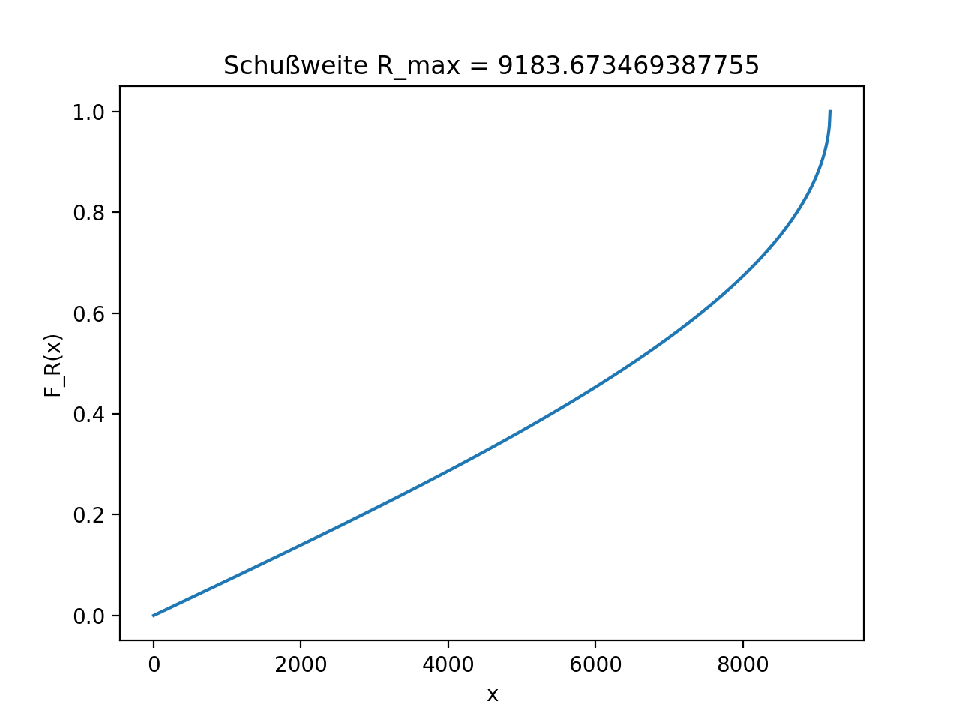
\epsfig{file=Abbildungen/schussweite-verteilung.pdf,scale=0.6}\\
   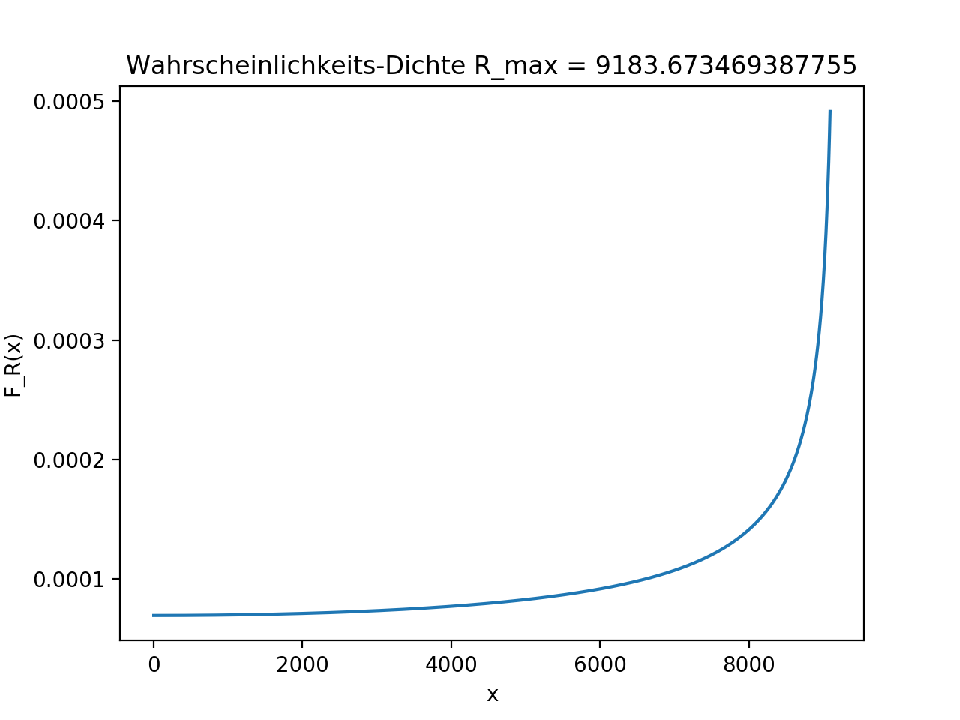
\epsfig{file=Abbildungen/schussweite-dichte.pdf,scale=0.6}
   \caption{Verteilungs-Funktion und Wahrscheinlichkeits-Dichte der SchussWeite.}
  \label{fig:reichweite}
\end{figure}

\noindent
Der n�chste Satz  verallgemeinert das obige Beispiel.  
\begin{Satz}[\blue{Variablen-Transformation}] \label{satz:vartrans} Es sei
  \begin{enumerate}
  \item $\mathcal{W}= \langle \Omega, \frak{A}, P \rangle$ ein Wahrscheinlichkeits-Raum,
  \item $X:\Omega \rightarrow [a,b]$ eine stetige Zufalls-Variable,
  \item $\varphi:[a,b] \rightarrow [c,d]$ eine streng monoton wachsende Funktion
  \item $\psi:[c,d] \rightarrow [a,b]$ die Umkehrfunktion von $\varphi$, also 
        \\[0.2cm]
        \hspace*{1.3cm}
        $\psi\bigl(\varphi(t)\bigr) = t$ \quad f�r alle $t\in [a,b]$,
  \item $Y:\Omega \rightarrow [c,d]$ eine Zufalls-Variable, die definiert ist durch 
        \\[0.2cm]
        \hspace*{1.3cm}
        $Y(\omega) := \varphi\bigl(X(\omega)\bigr)$.
  \end{enumerate}
  Dann gilt f�r die Wahrscheinlichkeits-Dichten $p_X$ und $p_Y$ die Beziehung 
  \\[0.2cm]
  \hspace*{1.3cm}
  $\ds p_Y(t) = p_X\bigl(\psi(t)\bigr) \cdot \frac{\mathrm{d} \psi}{\mathrm{d} t}$.
\end{Satz}

\proof Wir betrachten die Verteilungs-Funktion der Zufalls-Variable $Y$. Es gilt
\\[0.2cm]
\hspace*{1.3cm}
$
\begin{array}[t]{lcll}
 F_Y(t) & = & P(Y \leq t) \\[0.2cm]
& = & P(\varphi\circ X \leq t)    & \mbox{nach Definition von $Y$} \\[0.2cm]
& = & P\bigl(X \leq \psi(t)\bigr) & \mbox{denn $\psi$ ist Umkehrfunktion von $\varphi$} \\[0.2cm]
& = & F_X\bigl( \psi(t) \bigr)    & \mbox{nach Definition der Verteilungs-Funktion von $X$}
\end{array}
$
\\[0.2cm]
Wir haben also $F_Y(t) = F_X\bigl( \psi(t) \bigr)$.  Wenn wir diese Gleichung nach $t$ differenzieren,
erhalten wir die Behauptung mit Hilfe der Ketten-Regel: 
\\[0.2cm]
\hspace*{1.3cm}
$\ds p_Y(t) = \frac{\dx}{\dx t}F_Y(t) = \frac{\dx}{\dx t}F_X\bigl(\psi(t)\bigr) = 
   \frac{\dx F_X}{\dx \psi}\bigl(\psi(t)\bigr)\cdot \frac{\dx \psi}{\dx t} = p_X\bigl(\psi(t)\bigr)\cdot \frac{\dx \psi}{\dx t}$. 
\qed

\section{Erwartungswert und Varianz stetiger Zufalls-Variablen}
Es sei $\langle [a,b], \frak{A}, P\rangle$ ein Wahrscheinlichkeits-Raum und 
\\[0.2cm]
\hspace*{1.3cm}
$X: [a,b] \rightarrow [c,d]$ 
\\[0.2cm]
sei eine stetige Zufalls-Variable mit Wahrscheinlichkeits-Dichte $p_X$.
Wir �berlegen uns, wie wir die Definition des Erwartungswerts auf den kontinuierlichen Fall �bertragen k�nnen.
F�r eine diskrete Zufalls-Variable $Y$, deren Wertebereich sich als Menge der Form 
\\[0.2cm]
\hspace*{1.3cm}
$Y(\Omega) = \bigl\{ y_k \;\big|\; k \in \{1,\cdots,n\} \bigr\}$
\\[0.2cm]
schreiben l�sst, hatten wir seinerzeit die Formel 
\\[0.2cm]
\hspace*{1.3cm}
$\ds E[Y] = \sum\limits_{k=1}^n y_k \cdot P(Y=y_k)$
\\[0.2cm]
gefunden.  Da der Wertebereich der Zufalls-Variable $X$ kontinuierlich ist, k�nnen wir versuchen,
die m�glichen Werte von $X$ in viele kleine Intervalle der Form
\\[0.2cm]
\hspace*{1.3cm}
$[x_k, x_{k+1}]$ \quad mit $\ds x_k = c + \frac{k}{n} \cdot (d - c)$ f�r $k=0,\cdots,n-1$
\\[0.2cm]
aufzuteilen.  Jedes dieser Intervalle hat die L�nge 
\\[0.2cm]
\hspace*{1.3cm}
$\ds h = x_{k+1} - x_k = \frac{k+1}{n}\cdot(d-c) - \frac{k}{n}\cdot(d-c) = \frac{d-c}{n}$.
\\[0.2cm]
Wenn $n$ gro� ist, wird die L�nge $h$ diese Intervalle  sehr klein, so dass die Zahlen, die in dem
selben Intervall liegen, nahezu gleich sind.
Dann k�nnen  wir den Erwartungswert der Zufalls-Variable $X$ n�herungsweise durch
\\[0.2cm]
\hspace*{1.3cm}
$\ds E[X] \approx \sum\limits_{k=1}^n x_k \cdot P(x_{k-1} \leq X \leq x_k)$
\\[0.2cm]
berechnen.  Nun gilt 
\\[0.2cm]
\hspace*{1.3cm}
$\ds P(x_{k-1} \leq X \leq x_k) = \int_{x_{k-1}}^{x_k} p_X(x)\, \dx x$.
\\[0.2cm]
Also haben wir f�r den Erwartungswert 
\\[0.2cm]
\hspace*{1.3cm}
$\ds E[X] \approx \sum\limits_{k=1}^n x_k \cdot \int_{x_{k-1}}^{x_k} p_X(x)\, \dx x$
\\[0.2cm]
Hier k�nnen wir die Konstante $x_k$ in das Intergral hineinziehen und durch die Variable
$x$ ersetzen, denn innerhalb eines Intervalls $[x_{k-1},x_k]$ �ndert sich $x$ kaum, wenn
$n$ gro� und damit die Intervall-L�nge $x_{k} - x_{k-1} = \frac{d-c}{n}$ klein ist.  Dann haben wir 
\\[0.2cm]
\hspace*{1.3cm}
$\ds E[X] \approx \sum\limits_{k=1}^n  \int_{x_{k-1}}^{x_k} x \cdot p_X(x)\, \dx x = \int_{c}^{d} x \cdot p_X(x)\, \dx x$
\\[0.2cm]
Diese �berlegungen motivieren im Fall stetiger Zufalls-Variablen die Definition
des \blue{Erwartungswerts} einer stetigen Zufalls-Variable $X$ durch die Formel
\\[0.2cm]
\hspace*{1.3cm}
$\ds E[X] := \int_c^d x \cdot p_X(x) \dx x$.
\\[0.2cm]
Hier bezeichnen $c$ und $d$ den minimalen bzw.~maximalen Wert, den die Zufalls-Variable $X$ annehmen kann.
Die \blue{Varianz} einer stetigen Zufalls-Variable wird nun wie fr�her durch 
\\[0.2cm]
\hspace*{1.3cm}
$\ds \var[X] := E\Bigl[(X - E[X])^2\Bigr]$
\\[0.2cm]
definiert.  Setzen wir $\mu := E[X]$, so hei�t dies
\\[0.2cm]
\hspace*{1.3cm}
$\ds \var[X] = \int_c^d (x - \mu)^2 \cdot p_X(x) \dx x$. 

\exercise
Berechnen Sie Erwartungswert und Varianz der Zufalls-Variable $X$, falls f�r die Verteilungs-Funktion
$F_X$ gilt
\\[0.2cm]
\hspace*{1.3cm}
$F_X(t) = \left\{
\begin{array}[c]{ll}
 \ds 1 - \mathrm{e}^{-\lambda \cdot t} & \mbox{falls $t \geq 0$;} \\[0.2cm]
               0                        & \mbox{sonst.}
\end{array}
\right.
$
\eox

\solution
Zun�chst m�ssen wir die Wahrscheinlichkeits-Dichte $p_X$ berechnen.  Es gilt 
\\[0.2cm]
\hspace*{1.3cm}
$\ds p_X(t) = \frac{\dx}{\dx t} (1 - \mathrm{e}^{-\lambda \cdot t}) = \lambda \cdot \mathrm{e}^{-\lambda \cdot t}$ \quad f�r $x \geq 0$.
\\[0.2cm]
Damit erhalten wir f�r den Erwartungswert 
\\[0.2cm]
\hspace*{1.3cm}
$
\begin{array}[t]{lcl}  
E[X] 
& = & \ds  \int_0^\infty x \cdot \lambda \cdot \mathrm{e}^{-\lambda \cdot x} \dx x \\[0.3cm]
&   & \mbox{partielle Integration: $u(x) = x$ und $v'(x) = \lambda \cdot \mathrm{e}^{-\lambda \cdot x}$} \\
&   & \mbox{also:  \hspace*{2.2cm} $u'(x) = 1$ und $v(x) = - \mathrm{e}^{-\lambda \cdot x}$} \\[0.2cm]
& = & \ds \underbrace{-x \cdot \mathrm{e}^{-\lambda \cdot x}\Big|_0^\infty}_0 + 
      \int_0^\infty \mathrm{e}^{-\lambda \cdot x} \dx x                     \\[0.7cm]
&   & \mbox{denn $\lim\limits_{x \rightarrow \infty} x \cdot \mathrm{e}^{-\lambda \cdot x} = 0$} \\[0.3cm]
& = & \ds -\frac{1}{\lambda} \cdot \mathrm{e}^{-\lambda \cdot x} \Big|_0^\infty         \\[0.4cm]
& = & \ds \frac{1}{\lambda} 
\end{array}
$
\\[0.2cm]
F�r die Varianz finden wir entsprechend 
\\[0.2cm]
\hspace*{1.3cm}
$
\begin{array}[b]{lcl}  
\var[X] 
& = & \ds  \int_0^\infty \Bigl(x - \frac{1}{\lambda}\Bigr)^2  \cdot \lambda \cdot \mathrm{e}^{-\lambda \cdot x} \dx x \\[0.3cm]
&   & \mbox{partielle Integration: $u(x) = (x-\frac{1}{\lambda})^2$ und $v'(x) = \lambda \cdot \mathrm{e}^{-\lambda \cdot x}$} \\
&   & \mbox{also  \hspace*{2.3cm}  $u'(x) = 2\cdot(x - \frac{1}{\lambda})$ und $v(x) = - \mathrm{e}^{-\lambda \cdot x}$} \\[0.4cm]
& = & \ds - \Bigl(x - \frac{1}{\lambda}\Bigr)^2 \cdot \mathrm{e}^{-\lambda \cdot x}\Big|_0^\infty + 
      2 \cdot \int_0^\infty \Bigl(x - \frac{1}{\lambda}\Bigr) \cdot \mathrm{e}^{-\lambda \cdot x} \dx x                     \\[0.4cm]
& = & \ds \frac{1}{\lambda^2} + 2 \cdot \int_0^\infty \Bigl(x - \frac{1}{\lambda}\Bigr) \cdot \mathrm{e}^{-\lambda \cdot x} \dx x \\[0.4cm]
&   & \mbox{partielle Integration: $u(x) = x-\frac{1}{\lambda}$ und $v'(x) = \mathrm{e}^{-\lambda \cdot x}$} \\
&   & \mbox{also  \hspace*{2.3cm}  $u'(x) = 1$ und $v(x) = - \frac{1}{\lambda} \cdot \mathrm{e}^{-\lambda \cdot x}$} \\[0.4cm]
& = & \ds \frac{1}{\lambda^2} - \left(2 \cdot \Bigl(x-\frac{1}{\lambda}\Bigr) \cdot \frac{1}{\lambda} \cdot \mathrm{e}^{-\lambda \cdot x} \Big|_0^\infty\right) +
      \frac{2}{\lambda} \cdot \int_0^\infty \mathrm{e}^{-\lambda \cdot x} \dx x \\[0.4cm]
& = & \ds \frac{1}{\lambda^2} - \frac{2}{\lambda^2}  -
      \left(\frac{2}{\lambda^2} \cdot \mathrm{e}^{-\lambda \cdot x} \Big|_0^\infty\right) \\[0.4cm]
& = & \ds \frac{1}{\lambda^2} - \frac{2}{\lambda^2}  +
      \frac{2}{\lambda^2}  \\[0.4cm]
& = & \ds \frac{1}{\lambda^2}. 
\end{array}
$ 
\qed
\pagebreak

\remark
Ein Zufalls-Variable $X:\Omega \rightarrow \mathbb{R}$, deren Verteilungs-Funktion die Form
\\[0.2cm]
\hspace*{1.3cm}
$F_X(t) = \left\{
\begin{array}[c]{ll}
 \ds 1 - \mathrm{e}^{-\lambda \cdot t} & \mbox{falls $t \geq 0$,} \\[0.2cm]
               0                        & \mbox{sonst}
\end{array}
\right.
$
\\[0.2cm]
hat, nennen wir eine \href{https://de.wikipedia.org/wiki/Exponentialverteilung}{exponential-verteilte}
Zufalls-Variable mit Parameter $\lambda$ und schreiben
\\[0.2cm]
\hspace*{1.3cm}
$X \sim \mathrm{Exp}(\lambda)$.
\eoxs

\begin{Definition}[\href{https://de.wikipedia.org/wiki/Logistische_Verteilung}{Logistische Verteilung}]
  Eine Zufalls-Variable $X$ ist \blue{logistisch mit den Parametern $\mu$ und $\sigma$ verteilt}, falls die
  Verteilungs-Funktion $F_X$ die Form
  \\[0.2cm]
  \hspace*{1.3cm}
  $\ds F_X(x) = \frac{1}{\ds 1 + \exp\Bigl(-\frac{x-\mu}{s}\Bigr)}$
  \\[0.2cm]
  hat.  In diesem Fall schreiben wir
  $X \sim \mathrm{Log}(\mu, s)$.  \eoxs
\end{Definition}

\remark
Die logistische Verteilung spielt sp�ter in der \href{https://de.wikipedia.org/wiki/Logistische_Regression}{logistischen Regression}
und als \blue{Aktivierungsfunktion} bei den \href{https://de.wikipedia.org/wiki/K�nstliches_Neuron}{Neuronen} eines
\blue{neuronalen Netzes} eine wichtige Rolle. 
Abbildung \ref{fig:logistic-distribution.png} auf Seite \pageref{fig:logistic-distribution.png} zeigt die
Verteilungs-Funktion $F_X$ einer Zufalls-Variable $X$  mit $X \sim \mathrm{Log(1,0}$, die zugeh�rige
Wahrscheinlichkeits-Dichte $p_X$ ist Abbildung \ref{fig:logistic-distribution.png} auf Seite
\pageref{fig:logistic-distribution.png} geplottet.
\eoxs

\begin{figure}[t]
  \centering
   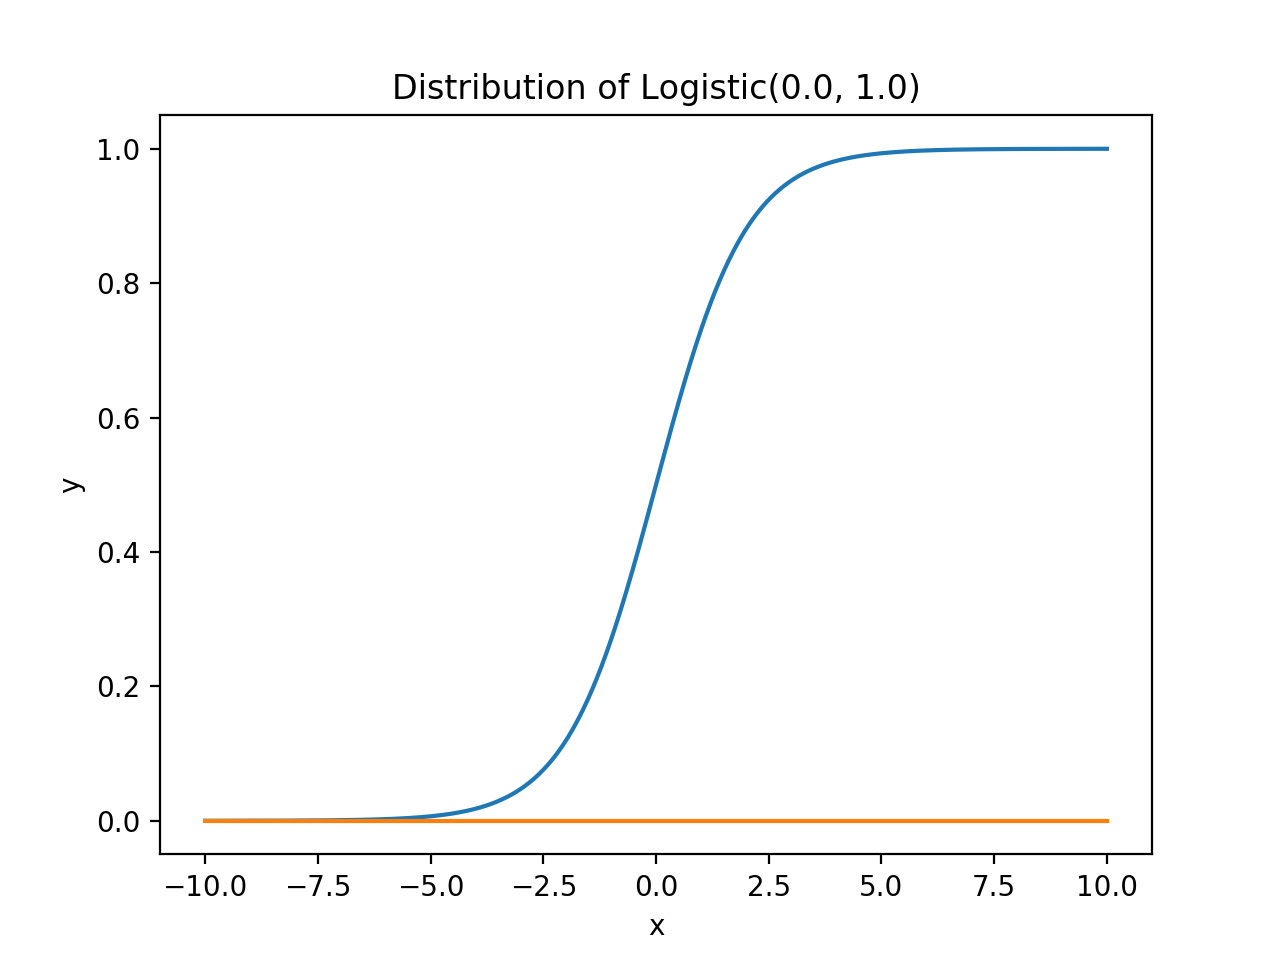
\epsfig{file=Abbildungen/logistic-distribution.png,scale=1.0}
   \caption{Verteilungs-Funktion und Wahrscheinlichkeits-Dichte einer logistisch verteilten Zufalls-Variable.}
  \label{fig:logistic-distribution.png}
\end{figure}

\begin{figure}[t]
  \centering
   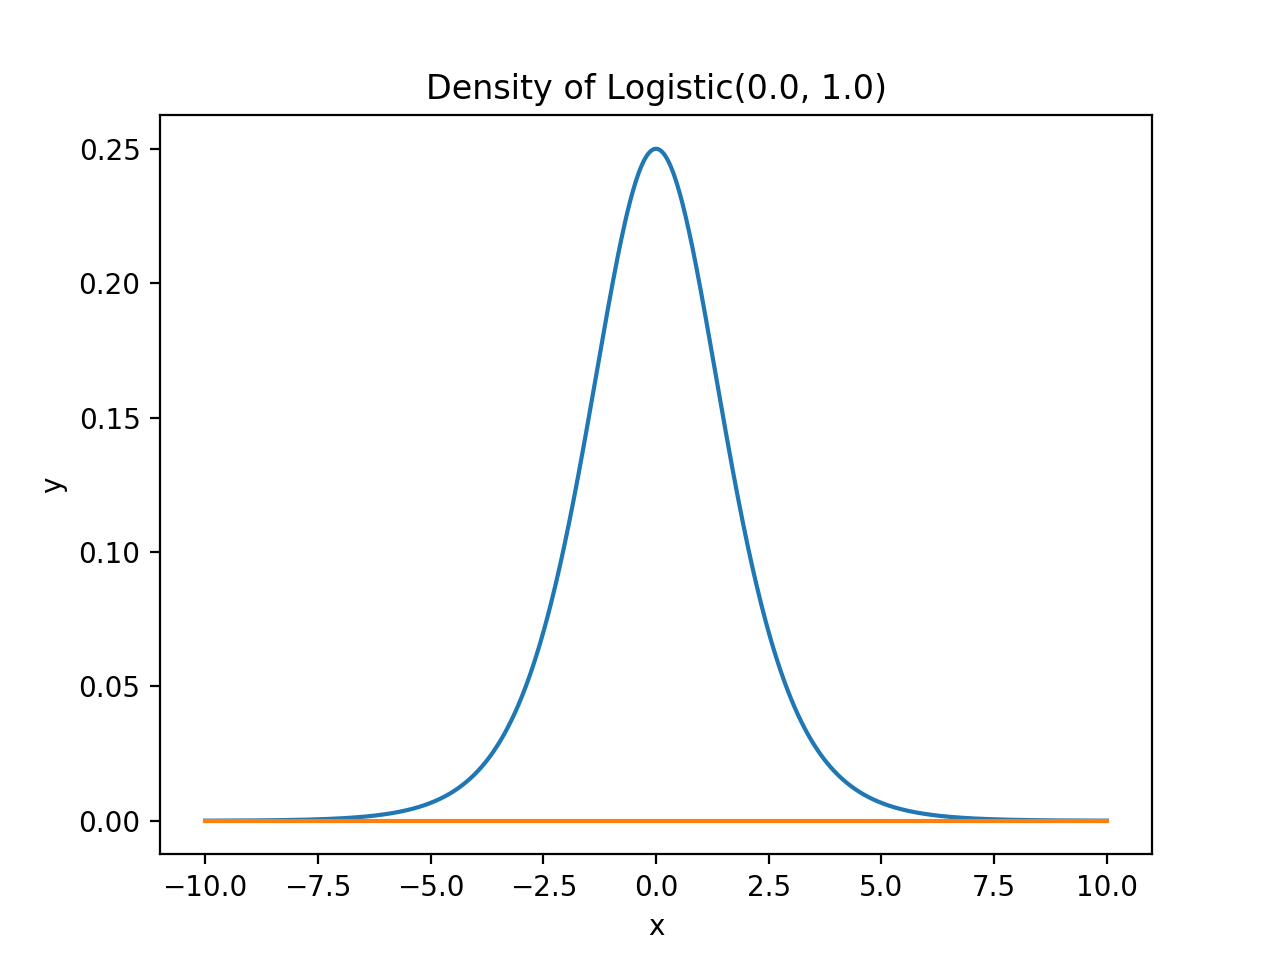
\epsfig{file=Abbildungen/logistic-density.png,scale=1.0}
   \caption{Verteilungs-Funktion und Wahrscheinlichkeits-Dichte einer logistisch verteilten Zufalls-Variable.}
  \label{fig:logistic-distribution.png}
\end{figure}

\exercise
Berechnen Sie den Erwartungswert und die Varianz einer logistisch verteilten Zufalls-Variable.
Beachten Sie dabei die folgenden \textbf{Hinweise}.
\begin{enumerate}[(a)]
\item Es ist am einfachsten, wenn Sie zun�chst den Erwartungs-Wert und die Varianz einer Zufalls-Variable $X$
      berechnen, f�r die $X \sim \mathrm{Log}(0,1)$ gilt.  Ist $Y$ dann eine Zufalls-Variable, f�r die
      $Y \sim \mathrm{Log}(\mu, s)$ gilt, so zeigt der Satz \ref{satz:vartrans}, dass $Y = \varphi \circ X$
      ist, falls Sie 
      \\[0.2cm]
      \hspace*{1.3cm}
      $\varphi(x) := s \cdot x + \mu$
      \\[0.2cm]
      definieren.  Mit Hilfe des Verschiebungs-Satzes k�nnen Sie anschlie�end $E[Y]$ und $\mathrm{Var}[Y]$ bestimmen.
\item Bei der Berechnung von Erwartungs-Wert und Varianz der Zufalls-Variable $X$ sollten Sie ausnutzen, dass die Funktion
      $p_X$ eine \blue{gerade Funktion} ist, es gilt also
      \\[0.2cm]
      \hspace*{1.3cm}
      $p_X(-x) = p_X(x)$.
      \\[0.2cm]
      In der Analysis hatten wir gesehen, dass
      \\[0.2cm]
      \hspace*{1.3cm}
      $\ds \int\limits_{-a}^a f(x) \mathrm{d}x = 2 \cdot \int\limits_0^a f(x) \mathrm{d}x$
      \\[0.2cm]
      ist, falls die Funktion $f$ gerade ist.  Ist die Funktion $f$ hingegen ungerade, gilt also $f(-x) = -f(x)$, 
      so haben wir
      \\[0.2cm]
      \hspace*{1.3cm}
      $\ds \int\limits_{-a}^a f(x) \mathrm{d}x = 0$.
\item Die Berechnung des Erwartungswerts $E[X]$ verl�uft ohne Komplikationen.  Bei der
      Berechnung der Varianz sollten Sie sich an die Formel f�r die geometrische Reihe erinnern:
      \\[0.2cm]
      \hspace*{1.3cm}
      $\ds\sum\limits_{n=0}^\infty q^n = \frac{1}{1-q}$  \quad falls $|q| < 1$ ist.   
      \\[0.2cm]
      Leiten wir diese Formel auf beiden Seiten nach $q$ ab, so erhalten wir
      \\[0.2cm]
      \hspace*{1.3cm}
      $\ds\sum\limits_{n=1}^\infty n \cdot q^{n-1} = \frac{1}{(1-q)^2}$  \quad falls $|q| < 1$ ist.   
      \\[0.2cm]
      Diese Formel m�ssen Sie an geeigneter Stelle r�ckw�rts, also von rechts nach links, anwenden.  
\item Schlie�lich sollten Sie sich daran erinnern, dass wir am Ende des zweiten Semesters die Formel
      \\[0.2cm]
      \hspace*{1.3cm}
      $\ds \sum\limits_{n=1}^\infty \frac{1}{n^2} = \frac{\;\pi^2}{6\,}$
      \\[0.2cm]
      bewiesen haben.  Aus dieser Formel l�sst sich die Summenformel
      \\[0.2cm]
      \hspace*{1.3cm}
      $\ds \sum\limits_{n=1}^\infty \frac{(-1)^{n+1}}{n^2} = \frac{\;\pi^2}{12\;}$
      \\[0.2cm]
      herleiten und $\mathrm{Var}[X]$ kann auf diese Summe zur�ck gef�hrt werden.
      \eoxs
\end{enumerate}

\begin{Satz} \label{satz:varianz}
  Es sei $X:\Omega \rightarrow [a,b]$ eine Zufalls-Variable mit Wahrscheinlichkeits-Dichte $p_X(t)$. 
  Dann kann die Varianz $\var[X]$ wie folgt berechnet werden: 
  \\[0.2cm]
  \hspace*{1.3cm}
  $\var[X] = E\bigl[X^2\bigr] - \bigl(E[X]\bigr)^2$.
\end{Satz}
\proof  Es sei $\ds\mu := E[X] = \int_a^b x \cdot p_X(x)\,\dx x$.  Dann gilt 
\\[0.2cm]
\hspace*{0.8cm}
$
\begin{array}[b]{lcl}
\var[X] & = & E\Bigl[\bigl(X-E[X]\bigr)^2\Bigr] \\[0.2cm]
& = & \ds
      \int_a^b (x - \mu)^2 \cdot p_X(x)\,\dx x \\[0.5cm]
& = & \ds
      \int_a^b \bigl(x^2 - 2 \cdot \mu \cdot x + \mu^2\bigr) \cdot p_X(x)\,\dx x \\[0.5cm]
& = & \ds
      \int_a^b x^2 \cdot p_X(x)\,\dx x \;-\;
      2 \cdot \mu \cdot \underbrace{\int_a^b x \cdot p_X(x)\,\dx x}_{E[X]} \;+\;
      \mu^2 \cdot \underbrace{\int_a^b  p_X(x)\,\dx x}_1 
      \\[0.7cm]
& = & \ds
      E\bigl[X^2\bigr] - 2 \cdot \mu^2 + \mu^2  
      \\[0.2cm]
& = & \ds
      E\bigl[X^2\bigr] - \bigl(E[X]\bigr)^2  
\end{array}
$ \qed
\pagebreak

\begin{Satz}[Verhalten des Erwartungswerts bei Variablen-Transformation] 
\label{satz:vartranserw} Es sei
  \begin{enumerate}
  \item $\mathcal{W}= \langle \Omega, \frak{A}, P \rangle$ ein Wahrscheinlichkeits-Raum,
  \item $X:\Omega \rightarrow [a,b]$ eine stetige Zufalls-Variable,
  \item $\varphi:[a,b] \rightarrow [c,d]$ eine stetige Funktion
  \item $Y:\Omega \rightarrow [c,d]$ eine Zufalls-Variable, die definiert ist durch 
        \\[0.2cm]
        \hspace*{1.3cm}
        $Y := \varphi \circ X$, \quad also \quad $Y(\omega) := \varphi\bigl(X(\omega)\bigr)$ \quad f�r alle $\omega \in \Omega$.
  \end{enumerate}
  Dann gilt f�r den Erwartungswert von $Y$ 
  \\[0.2cm]
  \hspace*{1.3cm}
  $\ds E[Y] = E[\varphi \circ X] = \int_a^b \varphi(x) \cdot p_X(x)\, \dx x$
\end{Satz}

\proof Wir setzen zus�tzlich voraus, dass die Funktion $\varphi$ streng monoton steigend
ist und dass $\psi:[c,d] \rightarrow [a,b]$ die Umkehrfunktion von $\varphi$ ist.
Nach dem Satz �ber Variablen-Transformation gilt dann
\\[0.2cm]
\hspace*{1.3cm}
$\ds p_Y(t) = p_X\bigl(\psi(t)\bigr) \cdot \frac{\dx \psi}{\dx t}$.
\\[0.2cm]
Nach Definition des Erwartungswerts gilt 
\\[0.2cm]
\hspace*{0.3cm}
$
\begin{array}[t]{lcll}
  E[Y] 
& = & \ds 
      \int_c^d y \cdot p_Y(y)\,\dx y & \mbox{nach Definition von $E[Y]$} \\[0.4cm] 
& = & \ds 
      \int_c^d y \cdot p_X\bigl(\psi(y)\bigr) \cdot \frac{\dx \psi}{\dx y}\,\dx y 
      & \mbox{nach Satz \ref{satz:vartrans} �ber Variablen-Transformationen}                  \\[0.4cm]
& = & \ds
      \int_c^d \varphi(\psi(y)) \cdot p_X\bigl(\psi(y)\bigr) \cdot \frac{\dx \psi}{\dx y}\,\dx y
      & \mbox{denn $\psi$ ist die Umkehrfunktion von $\varphi$}  \\[0.4cm]
& = & \ds
      \int_a^b \varphi(\psi) \cdot p_X(\psi) \dx \psi
      & \mbox{Substitutionsregel der Analysis}                    \\[0.4cm]
& = & \ds
      \int_a^b \varphi(x) \cdot p_X(x) \dx x
      & \hspace*{-1cm} \mbox{ob die Integrations-Variable $x$ oder $\psi$ hei�t, ist egal}
\end{array}
$
\\[0.2cm]
Im allgemeinen Fall kann der Beweis dadurch gef�hrt werden,
dass wir das Intervall $[a,b]$ in Intervalle zerlegen, in denen die Funktion
$\varphi$ streng monoton ist.
\qeds

\remark
Im Englischen hat dieser Satz den Namen
\href{https://en.wikipedia.org/wiki/Law_of_the_unconscious_statistician}{\emph{law of the unconscious statistician}},
abgek�rzt \blue{\textsc{Lotus}}.
\eoxs

\section{Moment-erzeugende Funktion}
In diesem Abschnitt f�hren wir ein Hilfsmittel ein, mit dem wir sp�ter die Wahrscheinlichkeits-Dichte f�r eine
Reihe wichtiger Zufalls-Variablen berechnen k�nnen.  Dieses Hilfsmittel ist die
\href{https://de.wikipedia.org/wiki/Momenterzeugende_Funktion}{moment-erzeugende Funktion} einer
Zufalls-Variable $X$.  Der Begriff der moment-erzeugenden Funktion wird au�erdem zum Beweis des 
\blue{zentralen Grenzwert-Satzes} ben�tigt.

\begin{Definition}[\href{https://de.wikipedia.org/wiki/Momenterzeugende_Funktion}{Moment-erzeugende Funktion}]
Es sei $X: [a,b] \rightarrow [c,d]$ eine stetige Zufalls-Variable.
Dann definieren wir die \blue{moment-erzeugende Funktion}
\\[0.2cm]
\hspace*{1.3cm}
$M_X: \mathbb{R} \rightarrow \mathbb{R}$
\\[0.2cm]
f�r alle $t \in \mathbb{R}$ als den folgenden Erwartungswert:
\\[0.2cm]
\hspace*{1.3cm}
$\ds M_X(t) := E\bigl[\exp(t \cdot X)\bigr] = \int_c^d \exp\bigl(t\cdot x\bigr) \cdot p_X(x)\, \dx x$.
\\[0.2cm]  
Dabei haben wir bei der letzten Gleichung Gebrauch von Satz \ref{satz:vartranserw} (\blue{\textsc{Lotus}}) gemacht.
\eoxs
\end{Definition}

\begin{Satz}[Verschiebungs-Satz f�r moment-erzeugende Funktionen]
Es sei $X:\Omega \rightarrow \mathbb{R}$ eine Zufalls-Variable, $a \in \mathbb{R}$ und $b\in \mathbb{R}\backslash \{0\}$.
Definieren wir die Zufalls-Variable $Y:\Omega \rightarrow \mathbb{R}$ als
\\[0.2cm]
\hspace*{1.3cm}
$\ds Y(\omega) = \frac{X(\omega) + a}{b}$,
\\[0.2cm]
so gilt 
\\[0.2cm]
\hspace*{1.3cm}
$\ds M_{Y}(t) = M_X\Bigl(\frac{\;t\;}{b}\Bigr) \cdot \exp\Bigl(\frac{a \cdot t}{b}\Bigr)$.
\end{Satz}

\exercise
Beweisen Sie den Verschiebungs-Satz f�r moment-erzeugende Funktionen.

\noindent
\textbf{Hinweis}: Verwenden Sie Satz \ref{satz:vartrans}.


\example
Es sei $\mu\in\mathbb{R}$ und $\sigma\in \mathbb{R}_+$.
Die Zufalls-Variable $X: \Omega \rightarrow \mathbb{R}$ habe die Wahrscheinlichkeits-Dichte
\\[0.2cm]
\hspace*{1.3cm}
$\ds p_X(x) = \frac{1}{\sqrt{2\cdot\pi\;}\!\cdot \sigma} \cdot \exp\left(- \frac{(x-\mu)^2}{2\cdot\sigma^2}\right)$ \quad mit $\sigma > 0$.
\\[0.2cm]
Eine solche Zufalls-Variable hei�t \href{https://de.wikipedia.org/wiki/Normalverteilung}{normal-verteilt} mit
Parametern $\mu$ und $\sigma$, wir schreiben 
\\[0.2cm]
\hspace*{1.3cm}
$X \sim \mathcal{N}(\mu, \sigma)$.
\\[0.2cm]
Wir werden sp�ter sehen, dass $\mu$ der Erwartungswert von $X$ ist.  Den
Parameter $\sigma$ werden wir als die Standard-Abweichung von $X$ erkennen.

\begin{figure}[t]
  \centering
   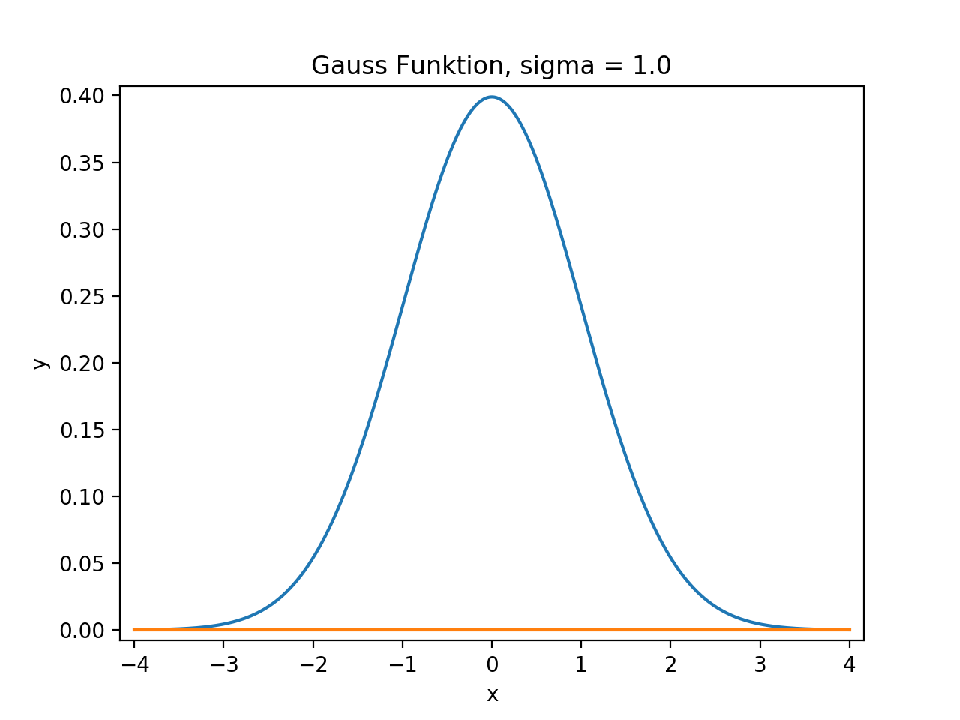
\epsfig{file=Abbildungen/gaussian.pdf,scale=1.0}
   \caption{Wahrscheinlichkeits-Dichte einer $\mathcal{N}(0,1)$ verteilten Zufalls-Variable.}
  \label{fig:gaussian}
\end{figure}

Abbildung \ref{fig:gaussian} auf Seite \pageref{fig:gaussian} zeigt die Wahrscheinlichkeits-Dichte einer Standard-Normal-Verteilung.  Abbildung
\ref{fig:zehn-deutsche-mark.png} auf Seite \pageref{fig:zehn-deutsche-mark.png} zeigt eine Banknote mit dem Portrait von
\href{https://en.wikipedia.org/wiki/Carl_Friedrich_Gauss}{Carl Friederich Gauss}, auf
dem diese Wahrscheinlichkeits-Dichte ebenfalls abgebildet ist.

\begin{figure}[!ht]
  \centering
   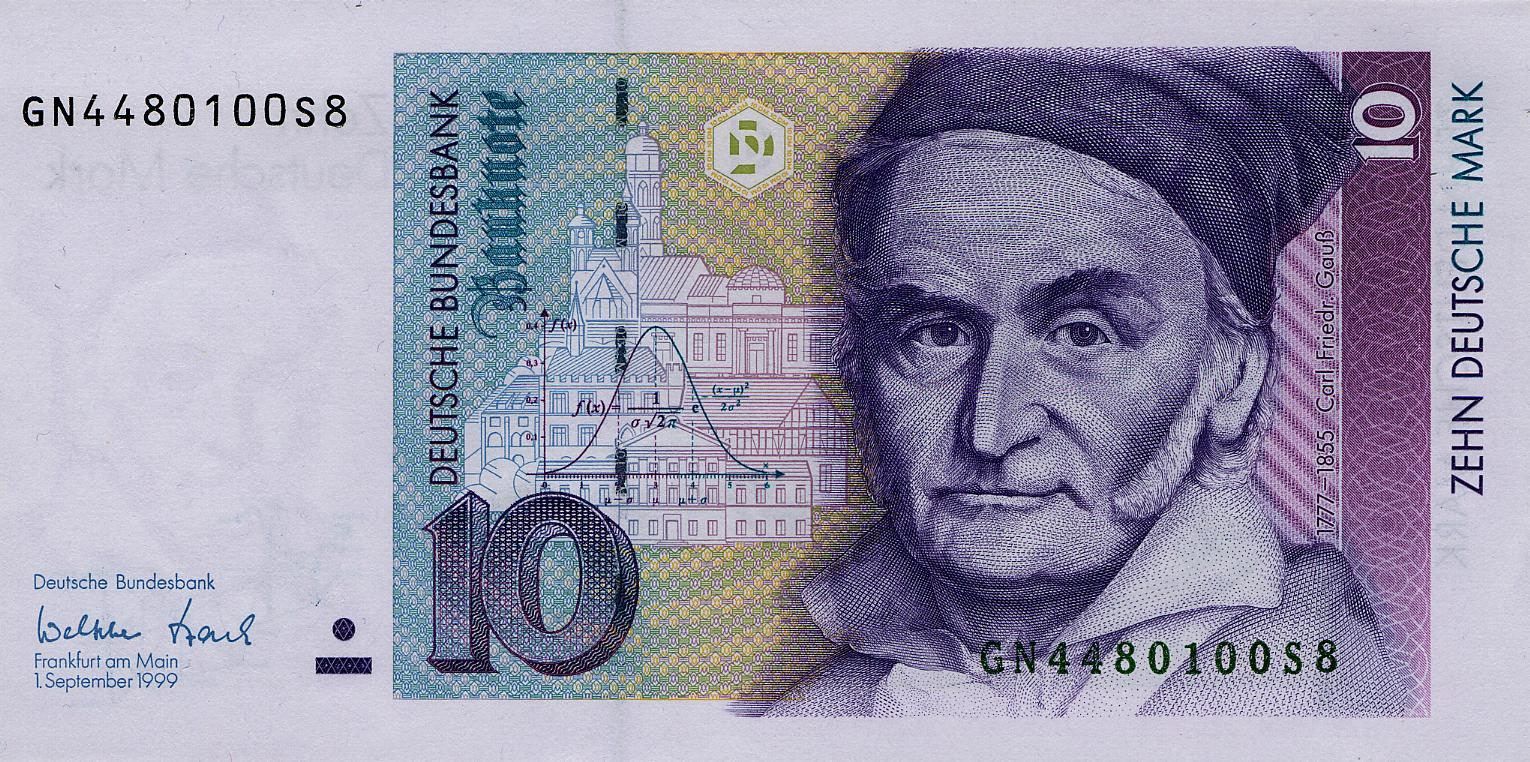
\epsfig{file=Abbildungen/zehn-deutsche-mark.png, scale=1.0}
   \caption{Vorderseite eines Zehn-Mark-Scheins.}
  \label{fig:zehn-deutsche-mark.png}
\end{figure}

Falls $Y$ eine Zufalls-Variable mit $Y \sim \mathcal{N}(0,1)$ ist, sprechen wir von einer \blue{standard-normal-verteilten} Zufalls-Variable.
Um $X$ und $Y$ in Beziehung zu setzen, definieren wir eine lineare Funktion $\varphi: \mathbb{R} \rightarrow \mathbb{R}$ durch
\\[0.2cm]
\hspace*{1.3cm}
$\ds \varphi(x) = \frac{x - \mu}{\sigma}$.
\\[0.2cm]
Die Umkehrfunktion $\psi$ von $\varphi$ ist dann
\\[0.2cm]
\hspace*{1.3cm}
$\ds \psi(y) = y\cdot \sigma + \mu$.
\\[0.2cm]
Dann gilt $Y := \varphi \circ X$, denn nach Satz \ref{satz:vartrans}
haben wir f�r die Wahrschein\-lichkeits-Dichte $p_Y$:
\\[0.2cm]
\hspace*{1.3cm}
$\ds p_Y(y) = p_X(y\cdot \sigma + \mu) \cdot \sigma =  \frac{1}{\sqrt{2\cdot\pi\;}} \cdot \exp\left(- \frac{y^2}{2}\right)$.
\\[0.2cm]
Die moment-erzeugende Funktion von $Y$ erhalten wir wie folgt:
\\[0.2cm]
\vspace*{\fill}

\pagebreak


\hspace*{1.3cm}

$
\begin{array}[t]{lcl}
 M_{Y}(t) 
& = & \ds
      \int_{-\infty}^\infty \exp(t\cdot x) \cdot \frac{1}{\sqrt{2\cdot\pi\;}} \cdot \exp\left(- \frac{x^2}{2}\right)\, \dx x 
      \\[0.5cm]
& = & \ds 
      \frac{1}{\sqrt{2\cdot\pi\;}} \cdot 
      \int_{-\infty}^\infty \exp(t\cdot x) \cdot \exp\left(- \frac{x^2}{2}\right)\, \dx x 
      \\[0.5cm]
& = & \ds
      \frac{1}{\sqrt{2\cdot\pi\;}} \cdot 
      \int_{-\infty}^\infty \exp\left(- \frac{1}{2}\cdot(x^2 - 2 \cdot t \cdot x) \right)\, \dx x 
      \\[0.5cm]
& = & \ds
      \frac{1}{\sqrt{2\cdot\pi\;}} \cdot 
      \int_{-\infty}^\infty 
      \exp\left(- \frac{1}{2}\cdot\bigl(x^2 - 2 \cdot t \cdot x + t^2 \bigr) + \frac{1}{2}\cdot t^2 \right)\, \dx x 
      \\[0.5cm]
& = & \ds
      \frac{1}{\sqrt{2\cdot\pi\;}} \cdot \exp\left(\frac{1}{2}\cdot t^2\right) \cdot
      \int_{-\infty}^\infty 
      \exp\left(- \frac{1}{2}\cdot\bigl(x - t\bigr)^2 \right)\, \dx x 
      \\[0.5cm]
& = & \ds
      \frac{1}{\sqrt{2\cdot\pi\;}} \cdot \exp\left(\frac{1}{2}\cdot t^2\right) \cdot
      \int_{-\infty}^\infty 
      \exp\left(- \frac{1}{2}\cdot y^2 \right)\, \dx y 
      \\[0.5cm]
&   & \mbox{mit der Variablen-Transformation $x \mapsto y + t$}
      \\[0.2cm]
& = & \ds
      \exp\left(\frac{1}{2}\cdot t^2\right) 
      \\[0.4cm]
&   & \mbox{denn $\ds \int_{-\infty}^\infty \exp\left(- \frac{1}{2}\cdot y^2 \right)\, \dx y = \sqrt{2\cdot\pi\,}$.}
      \\[0.4cm]
\end{array}
$
\\[0.2cm]
Zwischen der Zufalls-Variable $X$ und der Zufalls-Variable $Y$ besteht der Zusammenhang 
\\[0.2cm]
\hspace*{1.3cm}
$\ds X = \psi \circ Y = Y \cdot \sigma + \mu = \left(Y + \frac{\mu}{\sigma}\right)\cdot \sigma = 
   \left(Y + \frac{\mu}{\sigma}\right)\cdot \frac{1}{\textstyle \frac{1}{\sigma}}$
\\[0.2cm]
Nach dem Verschiebungs-Satz f�r moment-erzeugende Funktionen gilt daher 
\\[0.2cm]
\hspace*{1.3cm}
$
\begin{array}[b]{lcl} 
M_X(t) & = & \ds 
\exp(\mu \cdot t) \cdot M_{Y}\bigl(t \cdot \sigma\bigr) \\[0.3cm]
& = & \ds \exp(\mu \cdot t ) \cdot \exp\left( \frac{1}{2} \cdot t^2 \cdot \sigma^2\right) \\[0.3cm]
& = & \ds \exp\left( \frac{1}{2} \cdot t^2 \cdot \sigma^2 + \mu \cdot t\right)
\end{array}
$
\eoxs

\exercise
Beweisen Sie die beiden folgenden Eigenschaften einer normal-verteilten Zufalls-Variablen
$X\sim\mathcal{N}(\mu,\sigma)$: 
\\[0.2cm]
\hspace*{1.3cm}
$E\bigl[X\bigr] = \mu$ \quad und \quad $\var\bigl[X\bigr] = \sigma^2$.  \eoxs


\begin{Satz}[Eindeutigkeits-Satz] \label{satz:moment-eindeutig}
Es seien $X:\Omega \rightarrow \mathbb{R}$ und $Y: \Omega \rightarrow \mathbb{R}$ zwei Zufalls-Variablen und
f�r die moment-erzeugenden Funktionen $M_X$ und $M_Y$ gelte 
\\[0.2cm]
\hspace*{1.3cm}
$M_X(t) = M_Y(t)$ \quad f�r alle $t \in \mathbb{R}$.
\\[0.2cm]
Dann sind die Wahrscheinlichkeits-Dichten $p_X$ und $p_Y$ gleich:
\\[0.2cm]
\hspace*{1.3cm}
$p_X(t) = p_Y(t)$ \quad f�r alle $t \in \mathbb{R}$. \eox
\end{Satz}

\noindent
Der Beweis dieses Satzes gelingt, indem die moment-erzeugende Funktion einer Zufalls-Variable
auf die Fourier-Transformierte zur�ckgef�hrt wird.  Da wir die Fourier-Transformation
in der Analysis nicht mehr behandelt haben, k�nnen wir hier die Details dieses Beweises nicht 
diskutieren.  Trotzdem ist der Satz f�r unsere weitere Arbeit ein wichtiges Hilfsmittel,
denn er gestattet uns, die Wahrscheinlichkeits-Dichten bestimmter Zufalls-Variablen durch Berechnung 
der moment-erzeugenden Funktion zu berechnen.

\begin{Satz} \label{satz:moment-unabhaengig}
Es seien  $X:\Omega \rightarrow \mathbb{R}$ und $Y: \Omega \rightarrow \mathbb{R}$ zwei \red{unabh�ngige} Zufalls-Variablen.
Dann l�sst sich die moment-erzeugende Funktion der Zufalls-Variable $X + Y$ als Produkt der
moment-erzeugenden Funktionen von $X$ und $Y$ schreiben:
\\[0.2cm]
\hspace*{1.3cm}
$M_{X+Y}(t) = M_X(t) \cdot M_Y(t)$ \quad f�r alle $t\in \mathbb{R}$.
\end{Satz}

\proof  Es gilt 
\\[0.2cm]
\hspace*{1.3cm}
$
\begin{array}[b]{lcl}
      M_{X+Y}(t) 
& = & E\left[\exp\bigl(t\cdot(X+Y)\bigr)\right] \\[0.2cm]
& = & E\left[\exp(t\cdot X) \cdot \exp(t\cdot Y)\right] \\[0.2cm]
& = & E\left[\exp(t\cdot X)\right] \cdot E\left[\exp(t\cdot Y)\right] \\[0.2cm]
&   & \mbox{denn wenn $X$ und $Y$ unabh�ngig sind, } \\[0.2cm]
&   & \mbox{dann sind auch $\exp(t\cdot X)$ und $\exp(t\cdot Y)$ unabh�ngig} \\[0.2cm]
& = & M_X(t) \cdot M_Y(t) 
\end{array}
$
\\[0.2cm]
Hier haben wir im vorletzten Schritt ausgenutzt, dass mit $X$ und $Y$ auch die Zufalls-Variablen
$\exp(t\cdot X)$ und $\exp(t\cdot Y)$ unabh�ngig sind.  Genau wir im diskreten Fall auch gilt f�r den Erwartungswert
des Produkts unabh�ngiger Zufalls-Variablen $X$ und $Y$ die Gleichung 
\\[0.2cm]
\hspace*{1.3cm}
$E[X\cdot Y] = E[X] \cdot E[Y]$.
\qeds

\begin{Definition}[\href{https://de.wikipedia.org/wiki/Moment_(Stochastik)}{Moment}]
  Es sei $X$ eine Zufalls-Variable.  Das \blue{$n$-te Moment} von $X$ ist als
  \\[0.2cm]
  \hspace*{1.3cm}
  $\mathrm{Mt}(X,n) := E[X^n]$
  \\[0.2cm]
  definiert.  Gilt $\mu := E[X]$, so ist das \blue{$n$-te zentrale Moment} von $X$ als
  \\[0.2cm]
  \hspace*{1.3cm}
  $\mathrm{ZM}(X,n) := E\bigl[(X-\mu)^n\bigr]$
  \\[0.2cm]
  definiert. \qed
\end{Definition}

\begin{Definition}[\href{https://de.wikipedia.org/wiki/Schiefe_(Statistik)}{Schiefe}]
  Es sei $X$ eine Zufalls-Variable mit der Standard-Abweichung $\sigma$.  Die \blue{Schiefe} von $X$ ist dann
  als 
  \\[0.2cm]
  \hspace*{1.3cm}
  $\ds v(X) := \frac{\mathrm{ZM}(X, 3)}{\sigma^3} = \frac{E\bigl[(X-\mu)^3\bigr]}{\sigma^3}$
  \\[0.2cm]
  definiert.  Die Schiefe misst, wie unsymmetrisch die Verteilung der Zufalls-Variable $X$ ist.
\end{Definition}


\begin{Satz}
  Ist $f(t) = M_X(t)$ die moment-erzeugende Funktion der Zufalls-Variable $X$ und die Funktion sei $f$ in einer
  \href{https://de.wikipedia.org/wiki/Taylorreihe}{Taylor-Reihe} um $0$ entwickelbar.  Dann gilt
  \\[0.2cm]
  \hspace*{1.3cm}
  $\ds \mathrm{Mt}(X,n) = \frac{\mathrm{d}^n f}{\mathrm{d} t^n}(0)$.
\end{Satz}

\proof Es sei $X:\Omega \rightarrow [a,b]$.  Dann gilt 
\\[0.2cm]
\hspace*{1.3cm}
$
\begin{array}[b]{lcll}
      M_X(t) 
& = & \ds 
      \int_a^b \exp(t\cdot x) \cdot p_X(x)\, \dx x 
      \\[0.5cm]
& = & \ds 
      \int_a^b \sum\limits_{n=0}^\infty \frac{(t\cdot x)^n}{n!} \cdot p_X(x)\, \dx x & \quad
      \mbox{denn $\ds\exp(x) = \sum\limits_{n=0}^\infty \frac{x^n}{n!}$}
      \\[0.5cm]
& = & \ds 
      \sum\limits_{n=0}^\infty \frac{t^n}{n!} \cdot \int_a^b x^n \cdot p_X(x)\, \dx x 
      \\[0.5cm]
& = & \ds 
      \sum\limits_{n=0}^\infty \frac{t^n}{n!} \cdot E\bigl[X^n\bigr] 
      \\[0.5cm]
\end{array}
$
\\[0.2cm]
Auf der anderen Seite hat die Taylor-Reihe von $f(t)$ die Form 
\\[0.2cm]
\hspace*{1.3cm}
$\ds f(t) = \sum\limits_{n=0}^\infty \frac{t^n}{n!} \cdot f^{(n)}(0)$ 
\\[0.2cm]
Durch einen Koeffizienten-Vergleich der beiden Reihen erkennen wir, dass 
\\[0.2cm]
\hspace*{1.3cm}
$E[X^n] = f^{(n)}(0)$ \quad f�r alle $n \in \mathbb{N}$ gilt.  \qeds

\remark
An dieser Stelle sehen wir, wie n�tzlich die Kenntnis der Moment-erzeugenden Funktion einer Zufalls-Variable
$X$ ist, denn der Erwartungswert, die Varianz und die Schiefe von $X$ lassen sich aus den Momenten berechnen,
genauer gilt:
\begin{enumerate}[(a)]
\item $E[X] = \mathrm{Mt}(X, 1)$,
\item $\mathrm{Var}[X] = \mathrm{Mt}(X, 2) - \mathrm{Mt}(X, 1)^2$,
\item $\ds v(X) = \frac{\mathrm{ZM}(X,3)}{\mathrm{Var}[X]^{3/2}}$.

      Dabei kann das dritte zentrale Moment $\mathtt{ZM}(X,3)$ wie folgt aus dem ersten, zweiten und dritten
      Moment berechnet werden:
      \\[0.2cm]
      \hspace*{1.3cm}
      $\mathrm{ZM}(X,3) = \mathrm{Mt}(X,3)- 3 \cdot \mathrm{Mt}(X,2) \cdot \mathrm{Mt}(X,1) + 2 \cdot \mathrm{Mt}(X,1)^3$.
      \eoxs

      \exercise
      Beweisen Sie diese Formel.
\end{enumerate}

\begin{Satz}[Momente der Standard-Normal-Verteilung] \hspace*{\fill} \linebreak
  Es sei $X:\Omega \rightarrow \mathbb{R}$ eine standard-normal-verteilte Zufalls-Variable, es gelte also
  $X\sim\mathcal{N}(0,1)$.  Dann k�nnen die Momente von $X$ wie folgt berechnet werden:
  \begin{enumerate}
   \item $\mathrm{Mt}(X,2\cdot n + 1) = 0$ \quad f�r alle $n\in\mathbb{N}$.
   \item $\mathrm{Mt}(X,2\cdot n) = (2\cdot n-1)!!$ \quad f�r alle $n\in\mathbb{N}$ mit $n > 0$.

         Dabei ist f�r eine ungerade Zahl $2 \cdot m + 1$ der Ausdruck $(2\cdot m+1)!!$ als
         \\[0.2cm]
         \hspace*{1.3cm}
         $\ds (2\cdot m + 1)!! := 1 \cdot 3 \cdot 5 \cdot {\dots} \cdot (2\cdot m - 1) \cdot (2\cdot m + 1)
                                = \prod\limits_{k=0}^m (2 \cdot k + 1)
         $
         \\[0.2cm]
         definiert.  Dieser Ausdruck wird auch als \href{https://en.wikipedia.org/wiki/Double_factorial}{Doppel-Fakult�t} bezeichnet.
 \end{enumerate}
\end{Satz}

\proof
Wir haben fr�her f�r die Moment-erzeugende Funktion $M_X(t)$ einer standard-normal-verteilten Zufalls-Variable
$X$ den Ausdruck
\\[0.2cm]
\hspace*{1.3cm}
$\ds M_X(t) = \exp\biggl(\frac{t^2}{2}\biggr)$
\\[0.2cm]
gefunden.  Wir wissen, dass sich die Exponential-Funktion als
\\[0.2cm]
\hspace*{1.3cm}
$\ds\exp(x) = \sum\limits_{n=0}^\infty \frac{x^n}{n!}$
\\[0.2cm]
schreiben l�sst.  Setzen wir hier f�r $x$ den Ausdruck $t^2/2$ ein, so erhalten wir
\\[0.2cm]
\hspace*{1.3cm}
$\ds M_X(t) = \sum\limits_{n=0}^\infty \frac{t^{2\cdot n}}{n! \cdot 2^n} 
            = \sum\limits_{n=0}^\infty \frac{t^{2\cdot n}}{(2\cdot n)!} \cdot \frac{(2\cdot n)!}{n! \cdot 2^n}
            = \sum\limits_{n=0}^\infty \frac{t^{2\cdot n}}{(2\cdot n)!} \cdot (2\cdot n - 1)!! 
$,
\\[0.2cm]
denn Sie k�nnen durch eine elementare vollst�ndige Induktion zeigen, dass
\\[0.2cm]
\hspace*{1.3cm}
$\ds \frac{(2\cdot n)!}{n! \cdot 2^n} =  (2\cdot n - 1)!!$
\\[0.2cm]
gilt.  Der Beweis des letzten Satzes zeigt, dass das $n$-te Moment einer Zufalls-Variable $X$ gerade der
Koeffizient von $t^n/n!$ in der Taylor-Reihe von $M_X(t)$ ist.  Daraus folgt die Behauptung, denn in der Reihe
\\[0.2cm]
\hspace*{1.3cm}
$\ds \sum\limits_{n=0}^\infty \frac{t^{2\cdot n}}{(2\cdot n)!} \cdot (2\cdot n - 1)!! $ 
\\[0.2cm]
gibt es keine ungeraden Koeffizienten und der Koeffizient von $t^{2\cdot n}/(2\cdot n)!$ ist
offenbar $(2\cdot n - 1)!!$.
\qed

\section{Der zentrale Grenzwert-Satz}
Wir kommen nun zu dem wichtigsten Ergebnis der Wahrscheinlichkeits-Rechnung.
\begin{Satz}[Zentraler Grenzwertsatz]  
Es sei $(X_n)_{n\in\mathbb{N}}$ eine Folge unabh�ngiger stetiger Zufalls-Variablen, die alle dieselbe Wahrscheinlichkeits-Dichte haben,
es gilt also 
\\[0.2cm]
\hspace*{1.3cm}
$\forall m,n\in\mathbb{N}: p_{X_m}(t) = p_{X_n}(t)$.
\\[0.2cm]
Weiter gelte 
\\[0.2cm]
\hspace*{1.3cm}
$\mu = E[X_n]$ \quad und \quad $\sigma^2 = \var[X_n]$ \quad f�r alle $n \in \mathbb{N}$.
\\[0.2cm]
Definieren wir f�r $n \in \mathbb{N}$ die Zufalls-Variablen $S_n$ durch 
\\[0.2cm]
\hspace*{1.3cm}
$\ds S_n = \frac{1}{\sigma \cdot \sqrt{n}} \cdot \sum\limits_{k=1}^n \left(X_k - \mu\right)$,
\\[0.2cm]
so konvergieren die Wahrscheinlichkeits-Dichten $p_{S_n}$ der Zufalls-Variablen $S_n$ gegen die Normal-Verteilung, es gilt also
\\[0.2cm]
\hspace*{1.3cm}
$\ds \lim\limits_{n \rightarrow \infty} p_{S_n}(t) = \frac{1}{\sqrt{2\cdot\pi\,}} \cdot \exp\left(-\frac{1}{2} \cdot t^2\right)$.
\end{Satz}

\proof Wir f�hren den Beweis, indem wir zeigen, dass die moment-erzeugenden Funktionen 
$M_{S_n}$ der Zufalls-Variablen $S_n$ gegen die moment-erzeugende Funktion einer normal-verteilten Zufalls-Variable mit Mittelwert 
$0$ und Varianz $1$ konvergieren.  Die Behauptung folgt dann aus dem Eindeutigkeits-Satz \ref{satz:moment-eindeutig}. 
Es sei $f_k$ die moment-erzeugende Funktion der Zufalls-Variable
\\[0.2cm]
\hspace*{1.3cm}
 $\ds Y_k := \frac{X_k - \mu}{\sigma \cdot \sqrt{n}}$, \quad also
\\[0.2cm]
\hspace*{1.3cm}
$\ds f_k(t) := M_{Y_k}(t) = E\left[\exp\left(t \cdot \frac{1}{\sigma \cdot \sqrt{n}} \cdot (X_k - \mu)\right)\right]$.
\\[0.2cm]
Da die Zufalls-Variablen $X_n$ alle dieselbe Wahrscheinlichkeits-Dichte haben, sind auch die 
moment-erzeugenden Funktionen $M_{Y_k}$ f�r alle $k$ gleich:
\\[0.2cm]
\hspace*{1.3cm}
$\forall k,l \in \mathbb{N}: f_k = f_l$.
\\[0.2cm]
Daher k�nnen wir den Index $k$ bei der 
Funktion $f_k$ weglassen und 
\\[0.2cm]
\hspace*{1.3cm}
$f := f_k$
\\[0.2cm]
definieren.  F�r die moment-erzeugende Funktion $M_{S_n}$ finden wir jetzt das Folgende:
\\[0.2cm]
\hspace*{1.3cm}
$
\begin{array}[b]{lcl}
      M_{S_n}(t) 
& = & \ds
      E\left[ \exp\left(t\cdot \frac{1}{\sigma \cdot \sqrt{n}} \cdot \sum\limits_{k=1}^n \left(X_k - \mu\right)\right) \right] \\[0.5cm]
& = & \ds
      E\left[ \prod\limits_{k=1}^n \exp\left(t\cdot \frac{1}{\sigma \cdot \sqrt{n}} \cdot \left(X_k - \mu\right)\right) \right] \\[0.5cm]
& = & \ds
      \prod\limits_{k=1}^n E\left[ \exp\left(t\cdot \frac{1}{\sigma \cdot \sqrt{n}} \cdot \left(X_k - \mu\right)\right) \right] \\[0.5cm]
&   & \mbox{denn die Zufalls-Variablen $X_k$ sind unabh�ngig} \\[0.2cm]
& = & \ds
      \prod\limits_{k=1}^n f(t) \\[0.5cm]
& = & \ds
      f^n(t) \\[0.2cm]
\end{array}
$
\\[0.2cm]
In der Definition der moment-erzeugenden Funktion $f$ ersetzen wir die Exponential-Funktion durch die Taylor-Reihe 
\\[0.2cm]
\hspace*{1.3cm}
$\ds \exp(x) = \sum\limits_{i=0}^\infty \frac{x^i}{i!}$
\\[0.2cm]
und erhalten 
\\[0.2cm]
\hspace*{1.3cm}
$
\begin{array}[b]{lcl} 
      f(t) 
& = & \ds
      E\left[ \sum\limits_{i=0}^\infty \frac{1}{i!} \cdot \left(\frac{t}{\sigma \cdot \sqrt{n}}\right)^i \cdot (X_k - \mu)^i\right]
      \\[0.5cm]
& = & \ds
      \sum\limits_{i=0}^\infty \frac{1}{i!} \cdot \left(\frac{t}{\sigma \cdot \sqrt{n}}\right)^i \cdot E\bigl[(X_k - \mu)^i\bigr]
      \\[0.5cm]
& = & \ds
      1 \;+\; \frac{t}{\sigma \cdot \sqrt{n}} \cdot \underbrace{E[X_k - \mu]}_0
      \;+\; \frac{1}{2} \cdot \frac{t^2}{\sigma^2 \cdot n} \cdot E\bigl[(X_k - \mu)^2\bigr] \\[0.6cm]
&   & \ds+\; \frac{1}{6} \cdot \frac{t^3}{\sigma^3 \cdot n \cdot \sqrt{n}} \cdot E\bigl[(X_k - \mu)^3\bigr] \;+\; \cdots
      \\[0.5cm]
& \xrightarrow{\scriptsize n \rightarrow \infty} & \ds
      1 \;+\; \frac{1}{2} \cdot \frac{t^2}{\sigma^2 \cdot n} \cdot E\bigl[(X_k - \mu)^2\bigr] 
      \\[0.5cm]
& = & \ds
      1 \;+\; \frac{1}{2} \cdot \frac{t^2}{\sigma^2 \cdot n} \cdot \sigma^2 
      \\[0.5cm]
& = & \ds
      1 \;+\; \frac{1}{2} \cdot \frac{t^2}{n} 
      \\[0.5cm]
\end{array}
$
\\[0.2cm]
Dabei haben wir im letzten Schritt ausgenutzt, dass f�r $n \rightarrow \infty$ die Terme,
bei denen $n^{i/2}$ mit $i>2$ im Nenner steht, gegen�ber dem Term mit $\frac{1}{n}$ 
vernachl�ssigt werden k�nnen.  Daher haben wir 
\\[0.2cm]
\hspace*{1.3cm}
$
\begin{array}[b]{lcl}
  \lim\limits_{n \rightarrow \infty} M_{S_n}(t) 
& = & \ds \lim\limits_{n \rightarrow \infty} 
      \left(1 \;+\; \frac{1}{2} \cdot \frac{t^2}{n}\right)^n \\[0.3cm] 
& = & \ds 
      \exp\left(\frac{1}{2} \cdot t^2\right), \\[0.3cm] 
\end{array}
$
\\[0.2cm]
denn wir erinnern uns, dass wir in der Analysis gezeigt haben, dass
\\[0.2cm]
\hspace*{1.3cm}
$\ds\lim\limits_{n \rightarrow \infty} \Bigl(1 + \frac{x}{n}\Bigr)^n = \exp(x)$
\\[0.2cm]
gilt.  Die Funktion
\\[0.2cm]
\hspace*{1.3cm}
$\ds x \mapsto \exp\Bigl(\frac{1}{2} \cdot t^2\Bigr)$
\\[0.2cm]
ist aber gerade die moment-erzeugende Funktion einer Zufalls-Variable $X$, f�r die $X \sim \mathcal{N}(0,1)$
gilt.  Aus dem Eindeutigkeits-Satz \ref{satz:moment-eindeutig} f�r die moment-erzeugenden Funktionen folgt nun 
\\[0.2cm]
\hspace*{1.3cm}
$\ds \lim\limits_{n \rightarrow \infty} p_{S_n}(x) = \frac{1}{\sqrt{2\cdot\pi\,}} \cdot \exp\left(-\frac{1}{2}\cdot x^2\right)$.
\qed
\vspace*{0.3cm}

\noindent
Die Voraussetzungen des zentralen Grenzwertsatzes k�nnen noch abgeschw�cht werden.
Es ist nicht erforderlich, dass die einzelnen Zufalls-Variablen $X_k$ alle dieselbe Wahrscheinlichkeits-Dichte 
haben.  Im wesentlichen reicht es aus, wenn die Erwartungswerte und die Varianzen dieser 
Zufalls-Variablen beschr�nkt sind. Dar�ber hinaus muss dann noch eine weitere recht technische Bedingung erf�llt sein.
Der zentrale Grenzwertsatz ist der Grund daf�r, dass in der Praxis viele Zufalls-Variablen normal-verteilt sind.
Diese liegt einfach daran, dass viele Gr��en, die wir  beobachten, durch eine gro�e Zahl 
von Faktoren bestimmt werden.  Auch wenn die einzelnen Faktoren beliebig verteilt sind, so ist 
die Summe dieser Faktoren doch ann�hernd normal-verteilt.

\exercise
Die Zufalls-Variablen $X_1$ und $X_2$ seien normal-verteilt mit den Erwartungswerten  $\mu_1$ und $\mu_2$ und den Varianzen
$\sigma_1^2$ und $\sigma_2^2$, es gilt also
\\[0.2cm]
\hspace*{1.3cm}
$X_1 \sim \mathcal{N}(\mu_1, \sigma_1)$ \quad und \quad $X_2 \sim \mathcal{N}(\mu_2, \sigma_2)$.
\\[0.2cm]  
Au�erdem seien $X_1$ und $X_2$ \red{unabh�ngig}. 
Berechnen Sie die Wahrschein\-lichkeits-Dichte der Zufalls-Variable $X_1 + X_2$.
\vspace*{0.2cm}

\noindent
\textbf{Hinweis}:
Orientieren Sie sich am Beweis des zentralen Grenzwertsatzes. \eoxs

\section{Die \href{https://de.wikipedia.org/wiki/Chi-Quadrat-Verteilung}{Chi-Quadrat-Verteilung}}
In diesem Abschnitt gehen wir davon aus, dass $X_1$, $X_2$, $\cdots$, $X_n$  \red{unabh�ngige} 
Zufalls-Variablen sind, die alle einer standardisierten Normalverteilung gen�gen, f�r die einzelnen
Zufalls-Variablen $X_k$ gilt also $X_k \sim \mathcal{N}(0, 1)$ f�r alle $k=1,\cdots,n$.  Diesen Sachverhalt k�nnen wir auch als
\\[0.2cm]
\hspace*{1.3cm}
$\ds P(X_k \leq x) = \frac{1}{\sqrt{2\,\pi\,}} \cdot \int_{-\infty}^x
\exp\biggl(-\frac{t^2}{2}\biggr)\mathrm{d} t$ \quad f�r alle $k=1,\cdots,n$
\\[0.2cm]
schreiben.  Definieren wir die Zufalls-Variable $Z$ als 
\\[0.2cm]
\hspace*{1.3cm}
$\ds Z(\omega) = \sum\limits_{i=1}^n X_i^2(\omega)$,
\\[0.2cm]
so hat $Z$ eine \href{https://de.wikipedia.org/wiki/Chi-Quadrat-Verteilung}{$\chi^2$-Verteilung mit dem
Freiheitsgrad $n$}, wir schreiben
\\[0.2cm]
\hspace*{1.3cm}
$Z \sim \chi^2(n)$.
\\[0.2cm] 
Unser Ziel ist es, die Wahrscheinlichkeits-Dichte $p_Z$ f�r die Zufalls-Variable $Z$
zu berechnen.  Wir beginnen mit dem Spezialfall $n=1$.

\subsection{Die Chi-Quadrat-Verteilung mit dem Freiheitsgrad Eins}
Es sei $X$ eine Zufalls-Variable,
die der Standard-Normal-Verteilung gen�gt, f�r die Wahrscheinlichkeits-Dichte $p_X(x)$
gilt also
\\[0.2cm]
\hspace*{1.3cm}
$\ds p_X(x) = \frac{1}{\sqrt{2\pi}} \cdot \exp\Bigl(-\frac{x^2}{2}\Bigr)$.
\\[0.2cm]
Wir stellen uns die Frage, wie die Zufalls-Variable $X^2$ verteilt ist.  Wir berechnen 
zun�chst die kumulative Verteilungs-Funktion von $X^2$, die wir mit $F_{X^2}$ bezeichnen.  
Ist $\Omega$ der zu Grunde liegende Ergebnis-Raum, so haben wir 
\\[0.2cm]
\hspace*{1.3cm}
$
\begin{array}[t]{lcl}
\ds F_{X^2}(x) & = & \ds P(X^2 \leq x) \\[0.2cm]
 & = & \ds P\Bigl(\bigl\{ \omega \in \Omega \;\big|\; X^2(\omega) \leq x\bigr\} \Bigr) \\[0.3cm]
 & = & \ds P\Bigl(\bigl\{ \omega \in \Omega \;\big|\; -\sqrt{x} \leq X(\omega) \leq \sqrt{x}\bigr\} \Bigr) \\[0.3cm]
 & = & \ds P\Bigl(\bigl\{ \omega \in \Omega \;\big|\; X(\omega) \leq \sqrt{x}\bigr\} \;\backslash\;
                            \bigl\{ \omega \in \Omega \;\big|\; X(\omega) < -\sqrt{x}\bigr\} \Bigr) \\[0.3cm]
 & = & \ds \Phi\bigl(\sqrt{x}\bigr) - \Phi\bigl(-\sqrt{x}\bigr),
\end{array}
$
\\[0.2cm]
denn die Verteilungs-Funktion einer Zufalls-Variable mit Normalverteilung ist das
\href{https://de.wikipedia.org/wiki/Fehlerintegral}{gau�sche Fehlerintegral}
(benannt nach \href{https://en.wikipedia.org/wiki/Carl_Friedrich_Gauss}{Carl Friederich Gauss})
 \\[0.2cm]
\hspace*{1.3cm}
$\ds \Phi(x) := \frac{1}{\sqrt{2\cdot\pi\,}} \cdot \int\limits_{-\infty}^x \exp\bigl(-t^2/2\bigr)\, \mathrm{d}t$.
\\[0.2cm]
Auf Grund der Symmetrie des Integranden gilt die Gleichung
\\[0.2cm]
\hspace*{1.3cm}
$\Phi(x) + \Phi(-x) = 1$,
\\[0.2cm]
denn wir haben
\\[0.2cm]
\hspace*{1.3cm}
$\begin{array}[t]{lcl}
   1 & = & \ds \frac{1}{\sqrt{2\cdot\pi\,}} \cdot \int\limits_{-\infty}^\infty \exp\bigl(-t^2/2\bigr)\, \mathrm{d}t \\[0.6cm]
     & = & \ds \frac{1}{\sqrt{2\cdot\pi\,}} \cdot \int\limits_{-\infty}^x \exp\bigl(-t^2/2\bigr)\, \mathrm{d}t +
               \frac{1}{\sqrt{2\cdot\pi\,}} \cdot \int\limits_{x}^{\infty} \exp\bigl(-t^2/2\bigr)\, \mathrm{d}t    \\[0.6cm]
     & = & \ds \frac{1}{\sqrt{2\cdot\pi\,}} \cdot \int\limits_{-\infty}^x \exp\bigl(-t^2/2\bigr)\, \mathrm{d}t +
               \frac{1}{\sqrt{2\cdot\pi\,}} \cdot \int\limits_{-\infty}^{-x} \exp\bigl(-t^2/2\bigr)\, \mathrm{d}t    \\[0.6cm]
     & = & \ds \Phi(x) + \Phi(-x).       
\end{array}
$
\\[0.2cm]
Aus $\Phi(x) + \Phi(-x)$ folgt  $\Phi(-x) = 1 - \Phi(x)$ und damit finden wir f�r die Verteilungs-Funktion von $X^2$ die Gleichung 
\\[0.2cm]
\hspace*{1.3cm}
$F_{X^2}(x) = \Phi\bigl(\sqrt{x}\bigr) - \Phi\bigl(-\sqrt{x}\bigr) = \Phi\bigl(\sqrt{x}\bigr) - \bigl(1 -\Phi\bigl(\sqrt{x}\bigr) \bigr)  = 2 \cdot \Phi\bigl(\sqrt{x}\bigr) - 1$.
\\[0.2cm]
 Die Wahrscheinlichkeits-Dichte $p_{X^2}$ der Zufalls-Variable $X^2$ erhalten wir, indem wir die
Verteilungs-Funktion nach $x$ differenzieren.  Wegen
\\[0.2cm]
\hspace*{1.3cm}
$\ds \frac{\mathrm{d} \Phi}{\mathrm{d}x} = \frac{1}{\sqrt{2\cdot\pi\,}} \cdot \exp\bigl(-x^2/2\bigr)$
\\[0.2cm]
finden wir:
\\[0.2cm]
\hspace*{1.3cm}
$
\begin{array}[t]{lcl}
  p_{X^2}(x) & = & \ds \frac{\dx}{\dx x} \Bigl(2 \cdot \Phi\bigl(\sqrt{x}\bigr) - 1\Bigr) 
                  \\[0.5cm]
            & = & \ds 2 \cdot \frac{1}{2\cdot\sqrt{x}} \cdot \frac{1}{\sqrt{2\cdot\pi\,}} \cdot \exp(-x/2) 
                  \\[0.5cm]
            & = & \ds \frac{1}{\sqrt{2\cdot\pi\cdot x\,}} \cdot \exp(-x/2) 
\end{array}
$
\\[0.2cm]
Abbildung \ref{fig:chiSquare1} auf Seite \pageref{fig:chiSquare1} zeigt diese Funktion.

\begin{figure}[t]
  \centering
   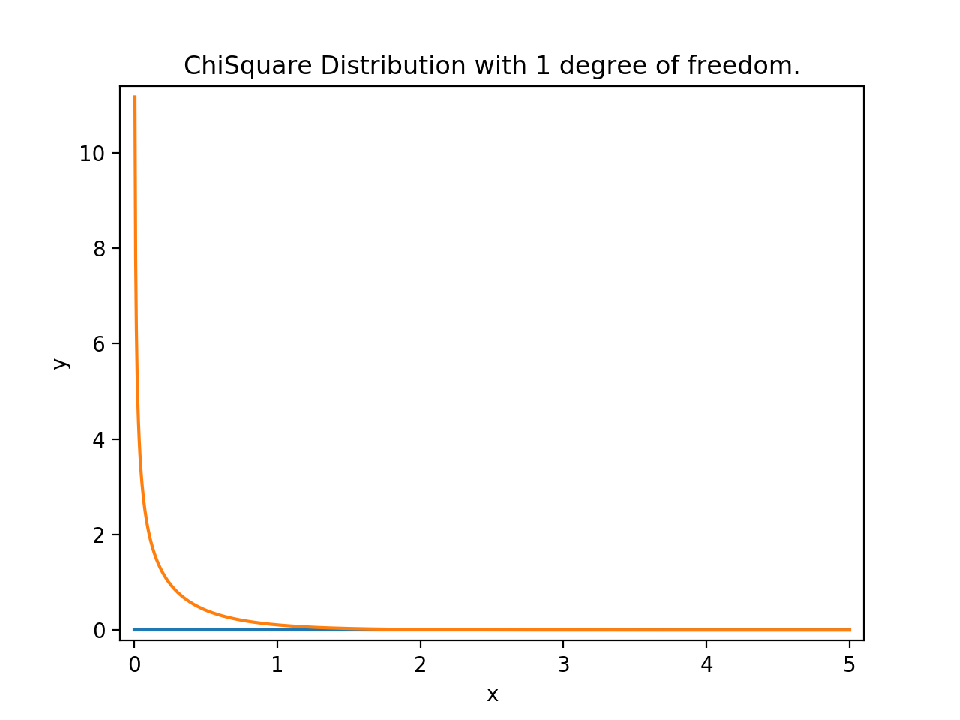
\epsfig{file=Abbildungen/chiSquare1.pdf,scale=1.0}
   \caption{Die $\chi^2$-Verteilung mit einem Freiheitsgrad.}
  \label{fig:chiSquare1}
\end{figure}

\exercise
Berechnen Sie die moment-erzeugende Funktion der Zufalls-Variable $X^2$.

\solution
Die Wahrscheinlichkeits-Dichte von $X^2$ haben wir eben berechnet.  Setzen wir das Ergebnis in die Definition
der Moment-Erzeugenden Funktion ein, so erhalten wir:
\\[0.2cm]
\hspace*{1.0cm}
$
\begin{array}[b]{lcl}
      M_{X^2}(t) 
& = & \ds
      \int_0^\infty \exp(t\cdot x) \cdot \frac{1}{\sqrt{2\pi\,}} \cdot \frac{1}{\sqrt{x}} \cdot \exp\left(-\frac{x}{2}\right)\,\dx x
      \\[0.5cm]
& = & \ds
      \frac{1}{\sqrt{2\pi\,}} \cdot \int_0^\infty \frac{1}{\sqrt{x}} \cdot \exp\left(t\cdot x -\frac{x}{2}\right)\,\dx x
      \\[0.4cm]
&   & \mbox{mit der Variablen-Transformation $x = y^2$, also $\dx x = 2\cdot y\, \dx y$ erhalten wir}  \\[0.2cm]
& = & \ds
      \frac{1}{\sqrt{2\pi\,}} \cdot \int_0^\infty \frac{1}{y} \cdot \exp\left( \Bigl(t - \frac{1}{2}\Bigr)\cdot y^2 \right)\cdot 2\cdot y\,\dx y
      \\[0.5cm]
& = & \ds
      \frac{2}{\sqrt{2\pi\,}} \cdot \int_0^\infty \exp\left( - \bigl(1 - 2 \cdot t\bigr)\cdot \frac{y^2}{2} \right)\,\dx y
      \\[0.4cm]
&   & \mbox{mit der Variablen-Transformation $\ds y = \frac{1}{\sqrt{1 - 2 \cdot t\;}} \cdot z$ wird daraus}  \\[0.3cm]
& = & \ds
      \frac{2}{\sqrt{2\pi\,}} \cdot \frac{1}{\sqrt{1 - 2 \cdot t\;}} \cdot \int_0^\infty \exp\left(-\frac{z^2}{2} \right)\,\dx z
      \\[0.4cm]
& = & \ds
      \frac{2}{\sqrt{2\pi\,}} \cdot \frac{1}{\sqrt{1 - 2 \cdot t\;}} \cdot \frac{1}{2} \cdot \sqrt{2\pi\;}
      \\[0.4cm]
&   & \mbox{denn $\ds \int_0^\infty \exp\left(-\frac{z^2}{2} \right)\,\dx z =
                  \frac{1}{2} \cdot\int_{-\infty}^\infty \exp\left(-\frac{z^2}{2} \right)\,\dx z =\frac{1}{2}\cdot \sqrt{2\pi\;}$} \\[0.5cm]
& = & \ds
      \frac{1}{\sqrt{1 - 2 \cdot t\;}}
\end{array}
$
\\[0.2cm]
Wir halten das Ergebnis fest: 
\begin{equation}
  \label{eq:chi-square2}
  \ds M_{X^2}(t) = \frac{1}{\sqrt{1 - 2 \cdot t\;}}
\end{equation}

\subsection{Der allgemeine Fall}
Um unser eigentliches Problem l�sen zu k�nnen,
ben�tigen wir zwei Definitionen.

\begin{Definition}[\href{https://de.wikipedia.org/wiki/Gammafunktion}{Gamma-Funktion}] 
Die \blue{Gamma-Funktion} ist f�r positive reelle Zahlen $x$ als das folgende Integral definiert:
\\[0.2cm]
\hspace*{1.3cm}
$\ds \Gamma(x) := \int_0^\infty t^{x-1} \cdot \mathrm{e}^{-t} \, \dx t$. \eoxs
\end{Definition}

\exercise
Weisen Sie die folgenden Eigenschaften der Gamma-Funktion nach:
\begin{enumerate}[(a)]
\item $\Gamma(1) = 1$.
\item $\Gamma\left(\frac{1}{2}\right) = \sqrt{\pi}$      .

      \textbf{Hinweis}: F�hren Sie das Integral durch eine geeignete Substitution
      auf das Integral
      \\[0.2cm]
      \hspace*{1.3cm} $\ds \int_0^\infty \exp\left(-\frac{1}{2}\cdot t^2\right)\, \dx t$ 
      \\[0.2cm]
      zur�ck.
\item $\Gamma(x + 1) = x \cdot \Gamma(x)$ \quad falls $x > 0$ ist. 

      \textbf{Hinweis}: Partielle Integration.
\item $\Gamma(n+1) = n!$ \quad f�r alle $n\in\mathbb{N}$.

      \textbf{Hinweis}: Vollst�ndige Induktion.

      Die letzte Eigenschaft zeigt, dass die Gamma-Funktion als eine Erweiterung
      der Fakult�ts-Funktion auf die positiven reellen Zahlen aufgefasst werden kann. 
      \eoxs
\end{enumerate}


\begin{Definition}[\href{https://de.wikipedia.org/wiki/Gammaverteilung}{Gamma-Verteilung}]
  Eine Zufalls-Variable $Y$ gen�gt einer \blue{Gamma-Verteilung mit Parametern $\alpha$ und $\beta$},
  falls f�r die Wahrscheinlichkeits-Dichte $p_Y$ gilt: 
  \\[0.2cm]
  \hspace*{1.3cm}
  $p_Y(x) = \left\{
  \begin{array}[c]{ll}
     \ds 
       \frac{1}{\beta^\alpha \cdot \Gamma(\alpha)} \cdot x^{\alpha-1} \cdot \exp\Bigl(\ds -\frac{x}{\beta}\Bigr)
     & \mbox{f�r $x>0$}; \\[0.5cm]
     0 & \mbox{f�r $x \leq 0$.}
  \end{array}\right.
  $ 
  \\[0.2cm]
  Die Parameter $\alpha$ und $\beta$ sind dabei positive reelle Zahlen.  
  In diesem Fall schreiben wir $Y \sim \Gamma(\alpha,\beta)$.
  \eoxs
\end{Definition}

\exercise
Nehmen Sie an, dass $Y$ eine gamma-verteilte Zufalls-Variable mit den Parametern $\alpha$ und $\beta$ ist, es
gilt also 
\\[0.2cm]
\hspace*{1.3cm}
$Y \sim \Gamma(\alpha, \beta)$
\\[0.2cm]
Berechnen Sie die moment-erzeugende Funktion von $Y$.

\solution
Nach Definition der moment-erzeugenden Funktion $p_Y$ gilt:
\\[0.2cm]
\hspace*{1.3cm}
$
\begin{array}[t]{lcl}
      M_Y(t) 
& = & \ds
      \int_0^\infty \exp(t\cdot x) \cdot p_Y(x)\, \dx x 
      \\[0.5cm]
& = & \ds
      \int_0^\infty \exp(t\cdot x) \cdot \frac{x^{\alpha-1} \cdot \exp\left(\textstyle -x/\beta\right)}{\beta^\alpha \cdot \Gamma(\alpha)}\, \dx x 
      \\[0.5cm]
& = & \ds
      \frac{1}{\beta^\alpha \cdot \Gamma(\alpha)} \cdot \int_0^\infty  x^{\alpha-1} \cdot \exp\left(-\frac{x}{\beta} + t\cdot x\right)\, \dx x 
      \\[0.5cm]
& = & \ds
      \frac{1}{\beta^\alpha \cdot \Gamma(\alpha)} \cdot \int_0^\infty x^{\alpha-1} \cdot \exp\left(-\Bigl(\frac{1}{\beta} - t\Bigr)\cdot x\right)\, \dx x 
\end{array}
$
\\[0.2cm]
Mit der Variablen-Transformation $\ds x = \frac{1}{\Bigl(\frac{1}{\beta} - t\Bigr)} \cdot y$ wird daraus:
\\[0.2cm]
\hspace*{1.3cm}
$
\begin{array}[t]{lcl}
      M_Y(t) 
      & = & \ds
      \frac{1}{\beta^\alpha \cdot \Gamma(\alpha)} \cdot \frac{1}{\Bigl(\frac{1}{\beta} - t\Bigr)} \cdot \frac{1}{\Bigl(\frac{1}{\beta} - t\Bigr)^{\alpha-1}} \cdot 
      \int_0^\infty y^{\alpha-1} \cdot \exp(-y)\, \dx y
      \\[0.6cm]
& = & \ds
      \frac{1}{\beta^\alpha \cdot \Gamma(\alpha)} \cdot \frac{1}{\Bigl(\frac{1}{\beta} - t\Bigr)^{\alpha}} \cdot 
      \Gamma(\alpha)
      \\[0.6cm]
& = & \ds
      \frac{1}{\beta^\alpha} \cdot \frac{1}{\Bigl(\frac{1}{\beta} - t\Bigr)^{\alpha}} 
      \\[0.6cm]
& = & \ds
      \frac{1}{\beta^\alpha} \cdot \left(\frac{\beta}{1 - \beta \cdot t}\right)^{\alpha}
      \\[0.4cm]
& = & \ds
      \bigl(1 - \beta \cdot t \bigr)^{-\alpha}.  \hspace*{2cm} \Box
\end{array}
$
\\[0.3cm]
Also hat die moment-erzeugende Funktion f�r eine Zufalls-Variable $Y$, die einer Gamma-Verteilung mit den
Parametern $\alpha$ und $\beta$ gen�gt, die Form
\begin{equation}
  \label{eq:chi-square3}
  M_Y(t) = (1 - \beta \cdot t)^{-\alpha}.
\end{equation}
Wir l�sen nun unser eigentliches Problem, n�mlich die Berechnung der Wahrscheinlichkeits-Dichte
einer Zufalls-Variable $Z$, die aus $n$ unabh�ngigen, standard-normal-verteilten Zufalls-Variablen
$X_i$ nach der Formel
\\[0.2cm]
\hspace*{1.3cm}
$\ds Z = \sum\limits_{i=1}^n X_i^2$
\\[0.2cm]
berechnet wird.  In diesem Fall schreiben wir
\\[0.2cm]
\hspace*{1.3cm}
$Z \sim \chi^2(n)$
\\[0.2cm]
und sagen, dass $Z$ eine \blue{$\chi^2$-Verteilung mit $n$ Freiheitsgraden} 
hat.  Wir berechnen zun�chst die moment-erzeugende Funktion $M_Z$ von $Z$.  Nach Satz \ref{satz:moment-unabhaengig}
und Gleichung (\ref{eq:chi-square2}) gilt 
\\[0.2cm]
\hspace*{1.3cm}
$\ds M_Z(t) = \Bigl(M_{X^2}(t)\Bigr)^n = (1 - 2 \cdot t)^{\textstyle -\frac{n}{2}}$
\\[0.2cm]
Nach Gleichung (\ref{eq:chi-square3}) hat eine Zufalls-Variable, die einer Gamma-Verteilung
mit den Parametern $\alpha = \frac{n}{2}$ und $\beta = 2$ gen�gt,
dieselbe moment-erzeugende Funktion.  Aus dem Eindeutigkeits-Satz \ref{satz:moment-eindeutig} f�r die moment-erzeugende 
Funktion folgt daher, dass die Wahrscheinlichkeits-Dichte der Zufalls-Variable $Z = \sum\limits_{i=1}^n X_i^2$ die Form 
\\[0.2cm]
\hspace*{1.3cm}
$\ds p_Z(x) = \frac{1}{A_n} \cdot x^{n/2-1} \cdot \exp\left( -\frac{x}{2}\right)$ \quad mit
$\ds A_n = 2^{n/2} \cdot \Gamma\left(\frac{n}{2}\right)$
\quad f�r $x > 0$ hat.
\\[0.2cm]
Wir formulieren dieses Ergebnis als Satz.  Vorher ben�tigen wir noch eine Definition.


\begin{Satz} \label{satz:chi-square-normal}
  Es seien $X_1$, $X_2$, $\cdots$, $X_n$ unabh�ngige Zufalls-Variablen, die
  standard-normal-verteilt sind.  Die Zufalls-Variable $Z$ sei definiert als 
  \\[0.2cm]
  \hspace*{1.3cm}
  $\ds Z := \sum\limits_{i=1}^n X_i^2$
  \\[0.2cm]
  Dann hat die Zufalls-Variable $Z$ die Wahrscheinlichkeits-Dichte 
  \\[0.2cm]
  \hspace*{1.3cm}
  $\ds p_Z(x) = \frac{1}{A_n} \cdot x^{n/2-1} \cdot \exp\left( -\frac{x}{2}\right)$ \quad mit
  $\ds A_n = 2^{n/2} \cdot \Gamma\left(\frac{n}{2}\right)$.
  \\[0.2cm]
  Zusammenfassend k�nnen wir auch sagen: Ist $Z$ eine Zufalls-Variable, so gilt
  \\[0.2cm]
  \hspace*{1.3cm}
  $\ds Z \sim \chi^2(n) \;\Rightarrow\; Z \sim \Gamma\Bigl(\frac{n}{2},2\Bigr)$. \eox
\end{Satz}

Die Abbildungen \ref{fig:chiSquare1.png}, \ref{fig:chiSquare2.png}, \ref{fig:chiSquare34510.png} und
\ref{fig:chiSquare30.png} auf den folgenden Seiten zeigen die Wahrscheinlichkeits-Dichten der
$\chi^2$-Verteilungen f�r die Freiheitsgrade $1$, $2$, $3$, $4$, $5$, $10$ und $30$.  Wir sehen, dass sich diese
Wahrscheinlichkeits-Dichten mit wachsender Zahl von Freiheitsgraden an die Wahrscheinlichkeits-Dichte einer
Normalverteilung ann�hern. Bei der Diskussion des $\chi^2$-Tests im n�chsten Kapitel ben�tigen wir die beiden
folgenden S�tze.

\begin{figure}[!ht]
  \centering
   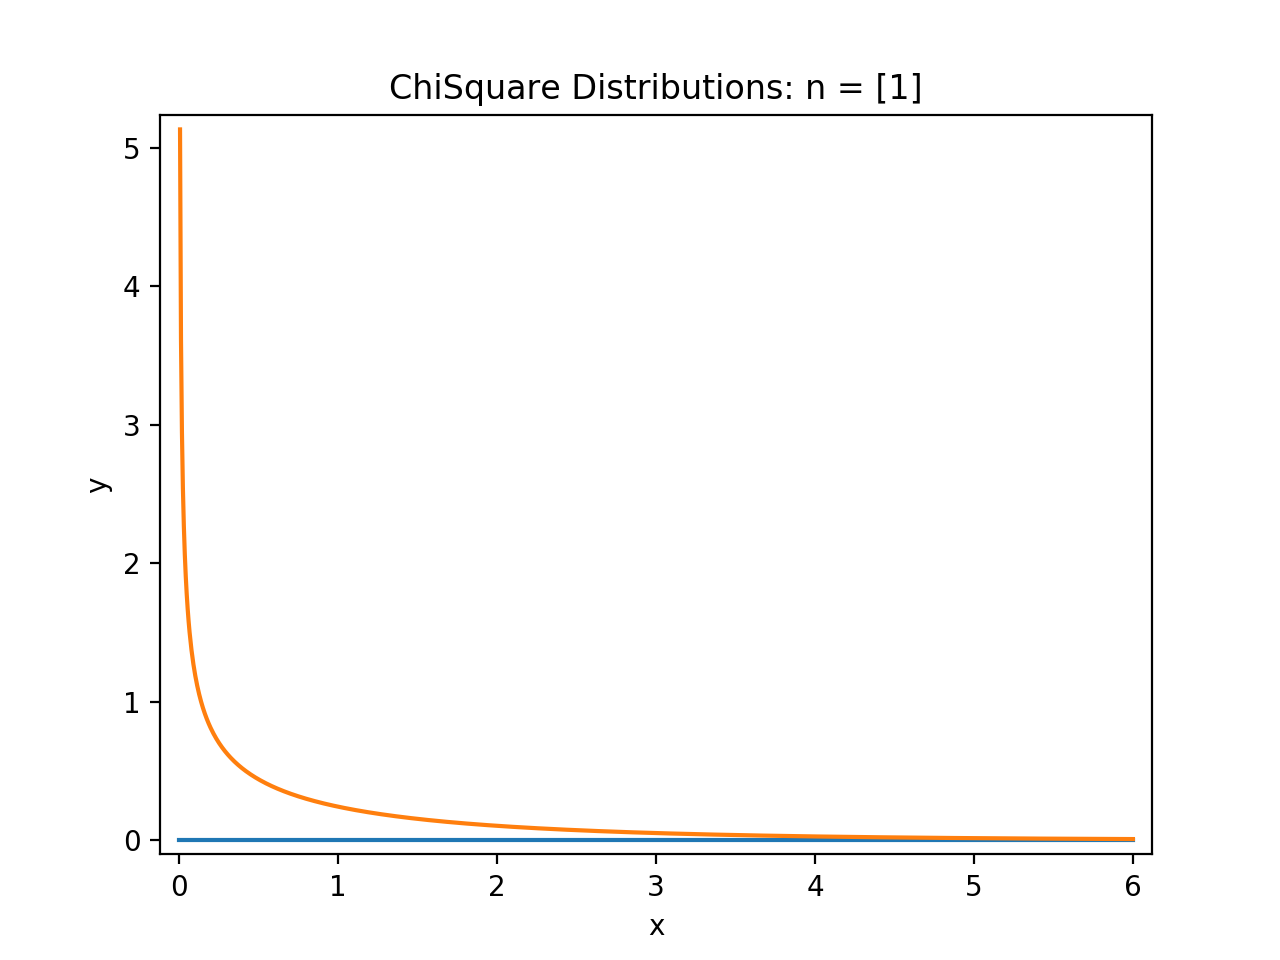
\epsfig{file=Abbildungen/chiSquare1.png,scale=0.9}
   \caption{Die $\chi^2$-Verteilungen mit dem Freiheitsgrad Eins.}
  \label{fig:chiSquare1.png}
\end{figure}


\begin{figure}[!ht]
  \centering
   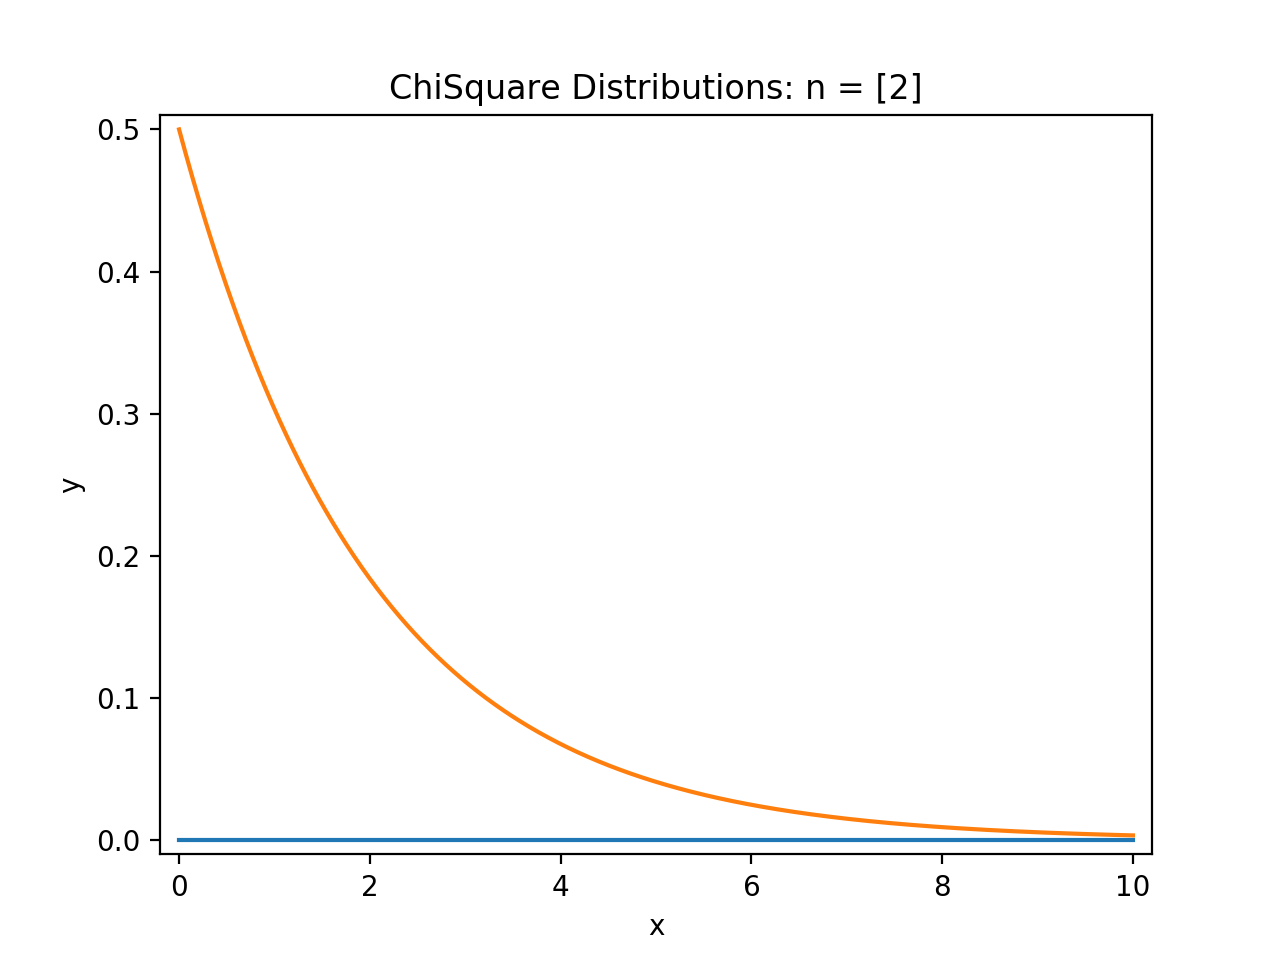
\epsfig{file=Abbildungen/chiSquare2.png,scale=0.9}
   \caption{Die $\chi^2$-Verteilungen mit dem Freiheitsgrad Zwei.}
  \label{fig:chiSquare2.png}
\end{figure}

\begin{figure}[!ht]
  \centering
   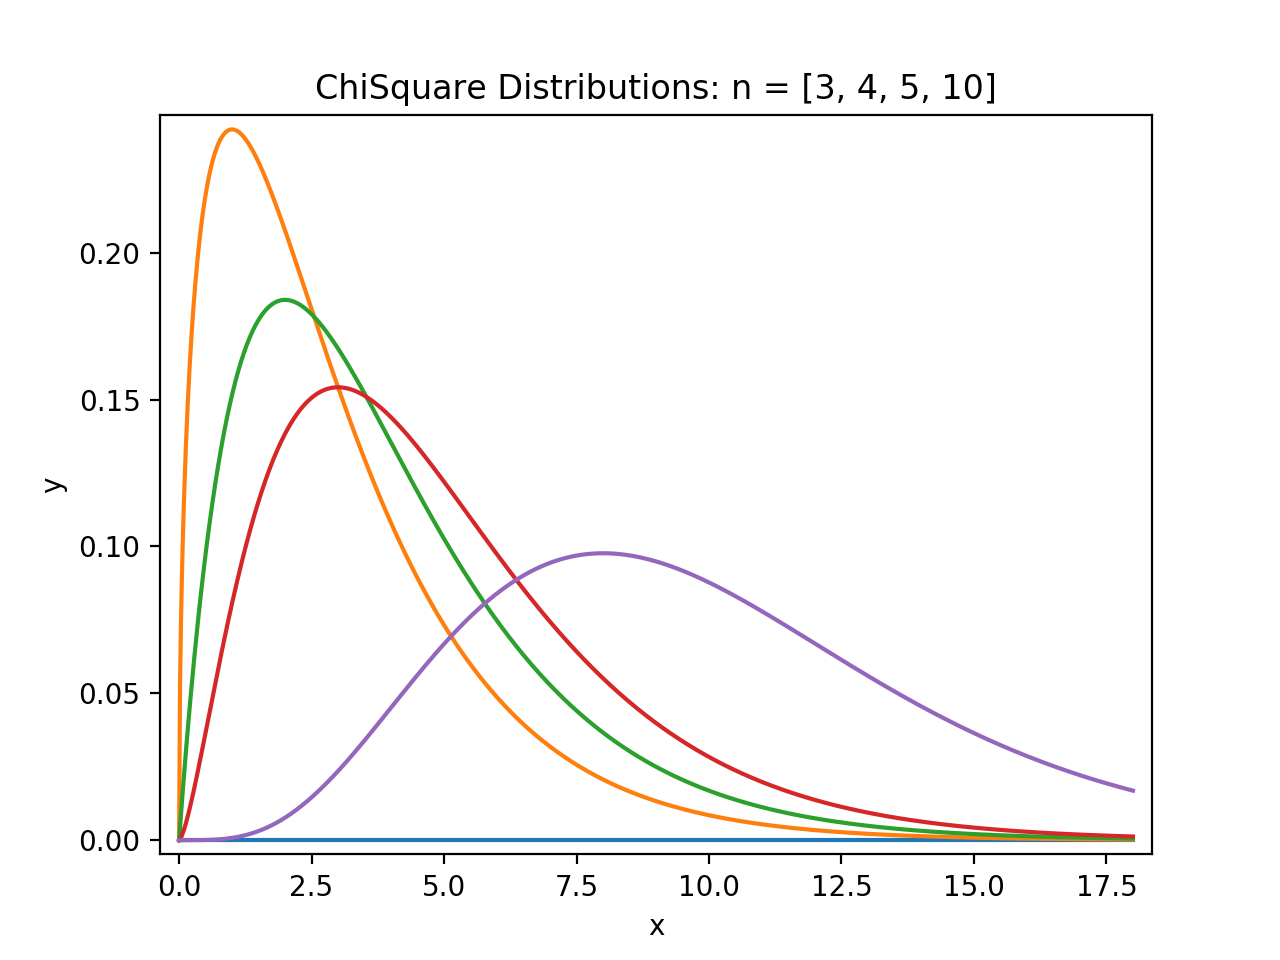
\epsfig{file=Abbildungen/chiSquare34510.png,scale=0.9}
   \caption{Die $\chi^2$-Verteilungen mit den Freiheitsgraden 3, 4, 5 und 10.}
  \label{fig:chiSquare34510.png}
\end{figure}

\begin{figure}[!ht]
  \centering
   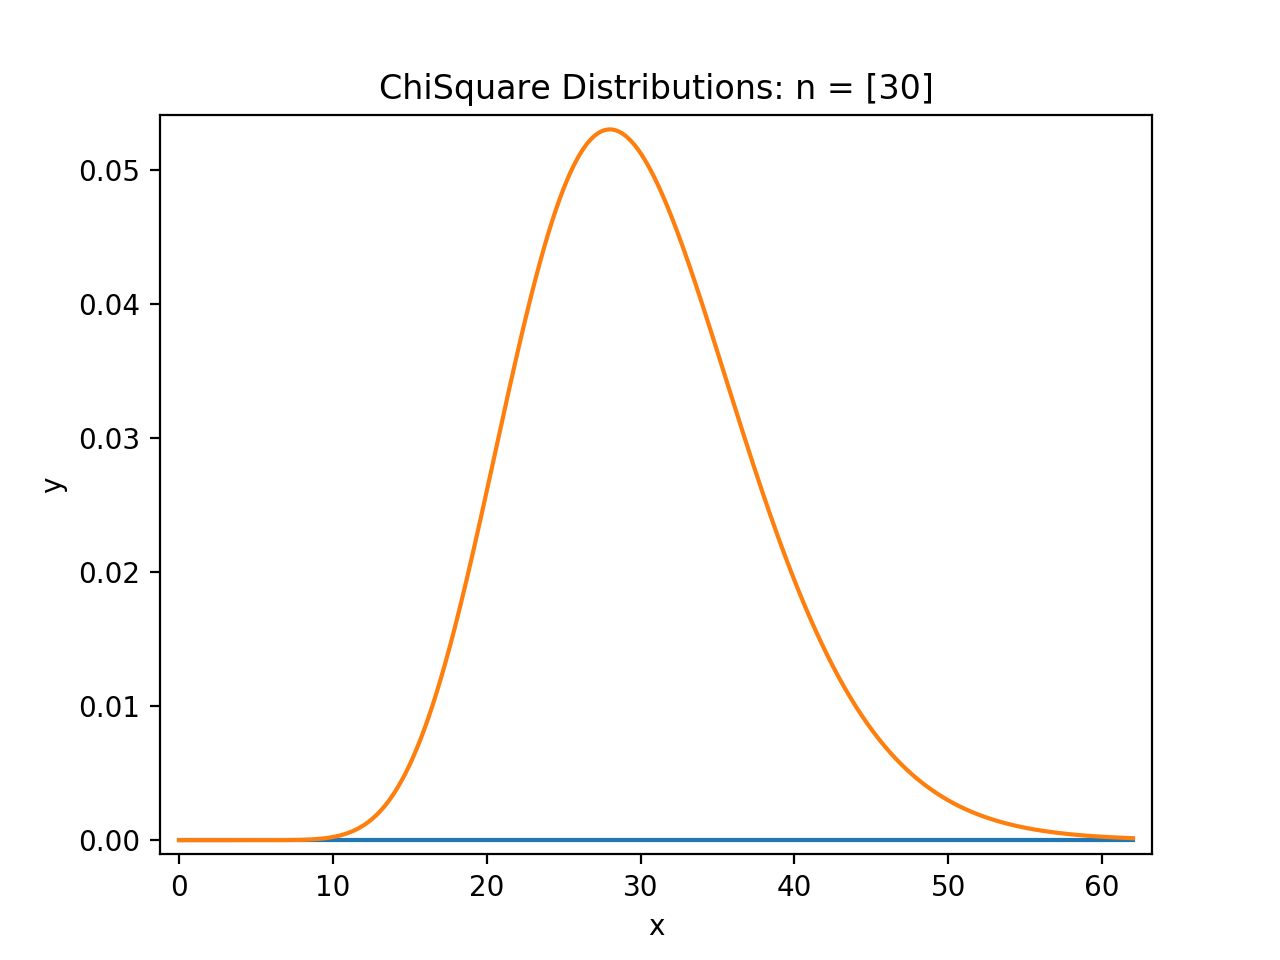
\epsfig{file=Abbildungen/chiSquare30.png,scale=0.9}
   \caption{Die $\chi^2$-Verteilungen mit dem Freiheitsgrad 30.}
  \label{fig:chiSquare30.png}
\end{figure}



\begin{Satz} \label{satz:chi-square-sum}
Es seien $U$, $V$ und $W$ Zufalls-Variablen mit folgenden Eigenschaften:
\begin{enumerate}
\item $U$ ist $\chi^2$-verteilt mit $m$ Freiheitsgraden,
\item $V$ ist $\chi^2$-verteilt mit $n$ Freiheitsgraden,
\item $U$ und $V$ sind unabh�ngig,
\item $W = U + V$.
\end{enumerate}
Dann gen�gt die Zufalls-Variable $W$ einer $\chi^2$-Verteilung mit $m+n$ Freiheitsgraden.
\end{Satz}

\proof  Aus dem Beweis des letzten Satzes k�nnen wir ablesen, wie die
moment-erzeugenden Funktionen  von $U$ und $V$ aussehen m�ssen.  Es gilt
\\[0.2cm]
\hspace*{1.3cm}
$\ds M_U(t) = (1- 2 \cdot t)^{\textstyle -\frac{m}{2}}$ \quad und \quad
$\ds M_V(t) = (1- 2 \cdot t)^{\textstyle -\frac{n}{2}}$.
\\[0.2cm]
Nach Satz \ref{satz:moment-unabhaengig} gilt daher f�r die moment-erzeugende Funktion $M_W$:
\\[0.2cm]
\hspace*{1.3cm}
$\ds M_W(t) = M_U(t) \cdot M_V(t) = (1- 2 \cdot t)^{\textstyle -\frac{m}{2}} \cdot (1- 2 \cdot
t)^{\textstyle -\frac{n}{2}} = (1- 2 \cdot t)^{\textstyle -\frac{m+n}{2}}$.
\\[0.2cm]
Dies ist aber genau die moment-erzeugende Funktion einer Zufalls-Variable, die einer
$\chi^2$-Verteilung mit $m+n$ Freiheitsgraden gen�gt.   Daher folgt die Behauptung aus
dem Eindeutigkeits-Satz \ref{satz:moment-eindeutig}. \qeds

\remark
Der obige Satz l�sst sich leicht auf die Summe von mehr als zwei
$\chi^2$-verteilten Zufalls-Variablen verallgemeinern.
Sind $U_1$, $\cdots$, $U_k$ unabh�ngige Zufalls-Variablen, so dass f�r alle $i=1,\cdots,k$
die Zufalls-Variable $U_i$  einer $\chi^2$-Verteilung mit $m_i$ Freiheitsgraden gen�gt, dann
gen�gt die Summe
\\[0.2cm]
\hspace*{1.3cm}
$W := \ds \sum\limits_{i=1}^k U_i$
\\[0.2cm]
einer $\chi^2$-Verteilung mit $m_1 + \cdots + m_k$ Freiheitsgraden.   Diese Aussage kann
mit Hilfe des letzten Satzes durch eine triviale Induktion nach $k$ gezeigt werden.
\qed

Der n�chste Satz zeigt, dass sich der letzte Satz auch umkehren l�sst.

\begin{Satz} \label{satz:chi-square4}
Es seien $U$, $V$ und $W$ Zufalls-Variablen mit folgenden Eigenschaften:
\begin{enumerate}
\item $U$ ist $\chi^2$-verteilt mit $m$ Freiheitsgraden,
\item $W$ ist $\chi^2$-verteilt mit $m+n$ Freiheitsgraden,
\item $U$ und $V$ sind unabh�ngig,
\item $W = U + V$.
\end{enumerate}
Dann gen�gt die Zufalls-Variable $V$ einer $\chi^2$-Verteilung mit $n$ Freiheitsgraden.
\end{Satz}

\proof
Wir f�hren den Beweis indem wir zeigen, dass die moment-erzeugende Funktion $M_V$ mit der
moment-erzeugenden Funktion einer $\chi^2$-verteilten Zufalls-Variable mit $n$
Freiheitsgraden �bereinstimmt.  

Aus den ersten beiden Voraussetzungen folgt, dass die
moment-erzeugenden Funktionen der Zufalls-Variablen $U$ und $W$ die folgende Gestalt haben: 
\\[0.2cm]
\hspace*{1.3cm}
$M_U(t) = (1- 2 \cdot t)^{\textstyle -\frac{m}{2}}$ \quad und \quad
$M_W(t) = (1- 2 \cdot t)^{\textstyle -\frac{m+n}{2}}$.
\\[0.2cm]
Nach Satz \ref{satz:moment-unabhaengig} gilt f�r die moment-erzeugenden Funktionen 
\\[0.2cm]
\hspace*{1.3cm}
$M_W(t) = M_U(t) \cdot M_V(t)$
\\[0.2cm]
Setzen wir hier die obigen Werte ein, so folgt 
\\[0.2cm]
\hspace*{1.3cm}
$(1- 2 \cdot t)^{\textstyle -\frac{m+n}{2}} = (1- 2 \cdot t)^{\textstyle -\frac{m}{2}}\cdot M_V(t)$
\\[0.2cm]
und das impliziert
\\[0.2cm]
\hspace*{1.3cm}
$M_V(t) = (1- 2 \cdot t)^{\textstyle -\frac{n}{2}}$.
\\[0.2cm]
Dies ist aber genau die moment-erzeugende Funktion einer $\chi^2$-verteilten
Zufalls-Variable vom Freiheitsgrad $n$.  Nach dem Eindeutigkeits-Satz \ref{satz:moment-eindeutig} hat die
Zufalls-Variable $V$ also eine $\chi^2$-Verteilung mit dem Freiheitsgrad $n$.
\qeds

\exercise
Nehmen Sie an, dass die Zufalls-Variable $Z$ einer $\chi^2$-Verteilung mit $n$ Freiheitsgraden gen�gt.
Berechnen Sie den Erwartungswert und die Varianz von $X$.

\noindent
\textbf{Hinweis}: Berechnen Sie zun�chst den Erwartungswert und die Varianz einer Zufalls-Variable $Z$, f�r die
$Z \sim \chi^2(1)$ gilt.
\eoxs

\exercise
Es sei $X$ eine Zufalls-Variable, f�r die $X \sim \chi^2(n)$ gilt.  An welcher Stelle nimmt die
Wahrscheinlichkeits-Dichte $p_X(x)$ ihren maximalen Wert an? 

\exercise
Es sei $X$ eine Zufalls-Variable, die einer $\chi^2$-Verteilung mit $4$ Freiheitsgraden
gen�gt.  Berechnen Sie die Verteilungs-Funktion $F_X$.
\eoxs



%%% Local Variables: 
%%% mode: latex
%%% TeX-master: "statistik"
%%% ispell-local-dictionary: "deutsch8"
%%% End: 

\chapter{Induktive Statistik}
Zwei wesentliche Aufgaben der Statistik sind das \blue{Sch�tzen von Parametern} und das
\blue{Testen von Hypothesen}.  Wir besprechen diese beiden Aufgaben in den beiden folgenden
Abschnitten. 

\section{Parameter-Sch�tzung}
Bisher haben wir uns im wesentlichen mit der Wahrscheinlichkeits-Rechnung besch�ftigt.
Bei der Wahrscheinlichkeits-Rechnung haben wir ein Model eines Prozesses in Form eines
Wahrscheinlichkeits-Raums.  
Mit Hilfe dieses Models berechnen wir dann die
Wahrscheinlichkeit f�r das Auftreten bestimmter Ereignisse.
Damit das m�glich ist, m�ssen uns die Parameter des Models bekannt sein.
Ein  solcher Parameter w�re beispielsweise der Erwartungswert $\lambda$ einer
Poisson-Verteilung oder der Erwartungswert $\mu$ und die Varianz $\sigma^2$ einer
normal-verteilten Zufalls-Variable.

Bei der Statistik ist die Situation anders:  Wir haben zwar meistens 
ebenfalls ein Model in Form eines Wahrscheinlichkeits-Raums, allerdings sind
diesmal die Parameter, welche die Verteilung der Zufalls-Variablen festlegen,  unbekannt.  Um diese Parameter
bestimmen zu k�nnen, beobachten wir Ereignisse und versuchen dann, mit Hilfe der Beobachtungen
die Parameter zu erschlie�en.  Wir haben diesen Prozess bereits in der Einf�hrung am
Beispiel der Ameisenz�hlung demonstriert.  Wir wollen diesen Prozess jetzt formalisieren.
Dazu ben�tigen wir einige Definitionen.

\begin{Definition}[\blue{Stichprobe}]
Gegeben sei eine endliche oder unendliche Menge $\Omega$, die wir im folgenden
als \blue{Population} (oder auch Grundgesamtheit) bezeichnen wollen. Ein
\blue{Merkmal} $X$ dieser Population ist eine Funktion 
\\[0.2cm]
\hspace*{1.3cm}
$X: \Omega \rightarrow \mathbb{R}$.
\\[0.2cm]
Eine \blue{Stichprobe} vom Umfang $n$ ist eine Teilmenge
\\[0.2cm]
\hspace*{1.3cm}
$\{ \omega_1, \cdots, \omega_n \} \subseteq \Omega$
\\[0.2cm]
die genau $n$ Elemente enth�lt. Setzen wir $x_i := X(\omega_i)$ f�r $i=1,\cdots,n$,
so werden die $x_i$ auch als \blue{Stichproben-Werte} bezeichnet.
\qed
\end{Definition}

\subsection{Sch�tzung des Erwartungswertes einer Zufalls-Variable}
Ist eine Stichprobe gegeben, so k�nnen wir versuchen, von der Stichprobe auf die
Grundgesamtheit zu schlie�en.  Ist beispielsweise $\{\omega_1,\cdots,\omega_n\}$ eine
Stichprobe und $X$ eine Zufalls-Variable, so wird der \blue{arithmetische Mittelwert} von $X$
mit $\overline{X}$ bezeichnet und durch
\\[0.2cm]
\hspace*{1.3cm}
$\ds \overline{X} := \frac{1}{n} \cdot \sum\limits_{i=1}^{n} X(\omega_i) = \frac{1}{n} \cdot \sum\limits_{i=1}^{n} x_i$
\\[0.2cm]
definiert.  Um das Verhalten von $\overline{X}$ mit den Mitteln der
Wahrscheinlichkeits-Rechnung untersuchen zu k�nnen, gehen wir aus von dem
Wahrscheinlichkeits-Raum 
\\[0.2cm]
\hspace*{1.3cm}
$\mathcal{V} = \langle \Omega, \frak{A}, P \rangle$.
\\[0.2cm]
Hier ist $\Omega$ die Population, $\frak{A}$ ist eine geeignete $\Sigma$-Algebra und $P$ ein Wahrscheinlichkeits-Ma�.
Dann definieren wir das $n$-fache kartesische Produkt 
\\[0.2cm]
\hspace*{1.3cm}
$\mathcal{W} := \mathcal{V}^n = \langle \Omega^n, \frak{A}^n, \widehat{P} \rangle$.
\\[0.2cm]
F�r ein Tupel von Ereignissen $\langle A_1, \cdots, A_n \rangle$ ist das Wahrscheinlichkeits-Ma� $\widehat{P}$ als 
\\[0.2cm]
\hspace*{1.3cm}
$\widehat{P}\bigl(\langle A_1, \cdots, A_n \rangle\bigr) := P(A_1) \cdot {\dots} \cdot P(A_n)$
\\[0.2cm]
definiert.  Dann k�nnen wir auf $\Omega^n$ die Zufalls-Variablen $X_i$  als 
\\[0.2cm]
\hspace*{1.3cm}
$X_i\bigl( \langle \omega_1, \cdots, \omega_i, \cdots, \omega_n \rangle\bigr) := X(\omega_i)$
\\[0.2cm]
definieren, $X_i$ ist also gerade die Anwendung  von $X$ auf die $i$-te Komponente der Stichprobe.
Die Wahrscheinlichkeits-Verteilungen der Zufalls-Variablen $X_i$ sind dann alle gleich der
Wahrscheinlichkeits-Verteilung der Zufalls-Variable $X$ auf dem urspr�nglichen Wahrscheinlichkeits-Raum $\mathcal{V}$.

Mit den $X_i$ ist auch der arithmetische Mittelwert $\overline{X}$ eine Zufalls-Variable auf
dem Stichproben-Raum $\Omega^n$. Wir k�nnen den Erwartungswert von $\overline{X}$
berechnen und finden 
\\[0.2cm]
\hspace*{1.3cm}
$
\begin{array}[t]{lcl}
 E\Bigl[\overline{X}\Bigr] 
& = & \ds
      E\left[ \frac{1}{n} \cdot \sum\limits_{i=1}^{n} X_i \right] \\[0.5cm]
& = & \ds  
      \frac{1}{n} \cdot \sum\limits_{i=1}^{n} E\left[X_i\right] \\[0.5cm]
& = & \ds  
      \frac{1}{n} \cdot \sum\limits_{i=1}^{n} E\left[X\right] \\[0.5cm]
& = & \ds  
      \frac{1}{n} \cdot E\left[X\right] \cdot \sum\limits_{i=1}^{n} 1 \\[0.5cm]
& = & \ds  
      \frac{1}{n} \cdot E\left[X\right] \cdot n \\[0.3cm]
& = & \ds  
      E\left[X\right].
\end{array}
$
\\[0.2cm]
Diese Rechnung zeigt, dass wir den arithmetischen Mittelwert einer Stichprobe benutzen
k�nnen um den Erwartungswert der Zufalls-Variable $X$ zu \blue{sch�tzen}.  
Ist 
\\[0.2cm]
\hspace*{1.3cm}
$\langle x_1, \cdots, x_n \rangle = \langle X(\omega_1), \cdots, X(\omega_n) \rangle$
\\[0.2cm]
ein \blue{Stichproben-Ergebnis}, so liefert uns dieses Ergebnis eine Sch�tzung des
Mittelwerts $E[X]$: 
\\[0.2cm]
\hspace*{1.3cm}
$\ds E[X] \approx \frac{1}{n} \cdot\sum\limits_{i=1}^{n} x_i = \overline{X}\bigl(\langle \omega_1, \cdots, \omega_n\rangle\bigr)$.
\\[0.2cm]
Wir untersuchen noch die Varianz der Zufalls-Variable $\overline{X}$, denn diese gibt uns
Aufschluss �ber die Genauigkeit unserer Sch�tzung.  Mit einer Rechnung, die analog zur
Herleitung des $\sqrt{n}$-Gesetzes ist, kann gezeigt werden, dass 
\\[0.2cm]
\hspace*{1.3cm}
$\ds \var\Bigl[\overline{X}\Bigr] = \frac{1}{n} \cdot \var[X]$ \quad und damit \quad
$\ds \sigma\Bigl[\overline{X}\Bigr] = \frac{1}{\sqrt{n}} \cdot \sigma[X]$ 
\\[0.2cm]
gilt.  Dies zeigt, wie die Genauigkeit mit wachsender Gr��e $n$ der Stichprobe zunimmt.
Der zentrale Grenzwertsatz zeigt, dass $\overline{X}$ f�r gro�e Werte von $n$ ann�hernd
normal verteilt ist.  In der Praxis zeigt sich, dass die Wahrscheinlichkeits-Verteilung
von $\overline{X}$ f�r $n \geq 30$ hinreichend gut durch eine Normal-Verteilung approximiert wird.

\subsection{Sch�tzung der Varianz einer Zufalls-Variable}
Als n�chstes suchen wir eine Zufalls-Variable, mit der wir die Varianz einer Zufalls-Variable
$X$ absch�tzen k�nnen.  Dazu definieren wir die \blue{Stichproben-Varianz} $S^2$ einer Stichprobe
vom Umfang $n$ als 
\\[0.2cm]
\hspace*{1.3cm}
$\ds S^2 := \frac{1}{n} \cdot \sum\limits_{i=1}^{n} \bigl(X_i - \overline{X}\bigr)^2$
\\[0.2cm]
Die Zufalls-Variable $S^2$ ist genau wie die Zufalls-Variable $\overline{X}$ auf dem
Stichproben-Raum $\Omega^n$ definiert.  Wir werden im folgenden 
die Wahrscheinlichkeits-Verteilung von
$S^2$ berechnen. 
In der Literatur wird die Stichproben-Varianz gelegentlich mit dem Faktor $\frac{1}{n-1}$
anstelle des Faktors $\frac{1}{n}$ definiert.  Wir folgen bei der obigen Definition der
Darstellung von Spiegel \cite{spiegel:2000}.  

Wir berechnen jetzt den Erwartungswert der Zufalls-Variable $S^2$.  
Dazu definieren wir 
\\[0.2cm]
\hspace*{1.3cm}
$\mu := E[X]$ \quad und \quad $\sigma^2 := \var[X]$.
\\[0.2cm]
Zun�chst formen wir die Summe $\sum\limits_{i=1}^{n} \bigl(X_i - \overline{X}\bigr)^2$ um:
\\[0.2cm]
\hspace*{1.3cm}
$
\begin{array}[t]{cl}
   & \ds
     \sum\limits_{i=1}^{n} \bigl(X_i - \overline{X}\bigr)^2 
     \\[0.5cm]
 = & \ds
     \sum\limits_{i=1}^{n} \bigl(X_i - \mu + \mu - \overline{X}\bigr)^2 
     \\[0.5cm]
 = & \ds
     \sum\limits_{i=1}^{n}\Bigl(\bigl(X_i - \mu\bigr)^2 + \bigl(\mu - \overline{X}\bigr)^2 + 2 \cdot (\mu - \overline{X}) \cdot (X_i - \mu)\Bigr)
     \\[0.5cm]
 = & \ds
     \sum\limits_{i=1}^{n} \bigl(X_i - \mu\bigr)^2 + 
     \sum\limits_{i=1}^{n} \bigl(\mu - \overline{X}\bigr)^2 + 
     \sum\limits_{i=1}^{n} 2 \cdot (\mu - \overline{X}) \cdot (X_i - \mu)
     \\[0.5cm]
 = & \ds
     \sum\limits_{i=1}^{n} \bigl(X_i - \mu\bigr)^2 + 
     \sum\limits_{i=1}^{n} \bigl(\mu - \overline{X}\bigr)^2 + 
     2 \cdot (\mu - \overline{X}) \cdot \sum\limits_{i=1}^{n} (X_i - \mu)
     \\[0.5cm]
 = & \ds
     \sum\limits_{i=1}^{n} \bigl(X_i - \mu\bigr)^2 + 
     n \cdot \bigl(\mu - \overline{X}\bigr)^2 + 
     2 \cdot (\mu - \overline{X}) \cdot n \cdot (\overline{X} - \mu)
     \\[0.5cm]
   & \mbox{denn $\sum\limits_{i=1}^{n} X_i = n \cdot \overline{X}$ und $\sum\limits_{i=1}^n \mu = n \cdot \mu$}  \\[0.2cm]
 = & \ds
     \sum\limits_{i=1}^{n} \bigl(X_i - \mu\bigr)^2 + 
     n \cdot \bigl(\mu - \overline{X}\bigr)^2 - 
     2 \cdot n \cdot \bigl(\mu - \overline{X}\bigr)^2 
     \\[0.5cm]
 = & \ds
     \sum\limits_{i=1}^{n} \bigl(X_i - \mu\bigr)^2 -
     n \cdot \bigl(\mu - \overline{X}\bigr)^2 
     \\[0.5cm]
\end{array}
$
\\[0.2cm]
Wir haben also 
\begin{equation}
  \label{eq:varianz-zerlegung}
 \ds \sum\limits_{i=1}^{n} \bigl(X_i - \overline{X}\bigr)^2 =
     \sum\limits_{i=1}^{n} \bigl(X_i - \mu\bigr)^2 - n \cdot \bigl(\mu - \overline{X}\bigr)^2 
\end{equation}
gezeigt.  Damit k�nnen wir $E\bigl[S^2\bigr]$ berechnen:
\\[0.2cm]
\hspace*{1.3cm}
$
\begin{array}[t]{lcl}
      E\bigl[ S^2 \bigr] 
& = & \ds
      \frac{1}{n} \cdot E\left[ \sum\limits_{i=1}^{n} \bigl(X_i - \overline{X}\bigr)^2  \right]
      \\[0.5cm]
& = & \ds
      \frac{1}{n} \cdot E\left[ \left(\sum\limits_{i=1}^{n} \bigl(X_i - \mu\bigr)^2 \right)- n \cdot \bigl(\mu - \overline{X}\bigr)^2 \right]
      \\[0.5cm]
& = & \ds
      \frac{1}{n} \cdot \left(\left(\sum\limits_{i=1}^{n} 
      E\left[ \bigl(X_i - \mu\bigr)^2 \right]\right) - n \cdot E\left[\bigl(\mu - \overline{X}\bigr)^2 \right]\right)
      \\[0.5cm]
& = & \ds
      \frac{1}{n} \cdot \left(\sum\limits_{i=1}^{n} E\left[ \bigl(X_i - \mu\bigr)^2 \right] \;-\;
      \sum\limits_{i=1}^{n} E\left[\bigl(\mu - \overline{X}\bigr)^2 \right]\right)
\end{array}
$
\\[0.2cm]
Nun gilt einerseits 
\\[0.2cm]
\hspace*{1.3cm}
$E\left[ \bigl(X_i - \mu\bigr)^2 \right] = E\left[ \bigl(X - \mu\bigr)^2 \right] = \sigma^2$,
\\[0.2cm]
denn die Zufalls-Variablen $X_i$ haben ja alle dieselbe Verteilung wie die Zufalls-Variable $X$,
andererseits haben wir wegen $E\Bigl[\overline{X}\Bigr] = E[X] = \mu$
\\[0.2cm]
\hspace*{1.3cm}
$\ds E\left[\bigl(\mu - \overline{X}\bigr)^2 \right] = \var\Bigl[\overline{X}\Bigr] = \frac{1}{n} \cdot \sigma^2$.
\\[0.2cm]
Das ergibt insgesamt 
\\[0.2cm]
\hspace*{1.3cm}
$
\begin{array}[t]{lcl}
      E\bigl[ S^2 \bigr] 
& = & \ds
      \frac{1}{n} \cdot \left(\sum\limits_{i=1}^{n} E\left[ \bigl(X_i - \mu\bigr)^2 \right] \;-\;
      \sum\limits_{i=1}^{n} E\left[\bigl(\mu - \overline{X}\bigr)^2 \right]\right)
      \\[0.5cm]
& = & \ds
      \frac{1}{n} \cdot\left( \sum\limits_{i=1}^{n} \sigma^2 \;-\;
      \sum\limits_{i=1}^{n} \frac{1}{n} \cdot \sigma^2 \right)
      \\[0.5cm]
& = & \ds
      \frac{1}{n} \cdot\left( n \cdot  \sigma^2 - \sigma^2 \right)
      \\[0.5cm]
& = & \ds
      \frac{n-1}{n} \cdot \sigma^2 
      \\[0.5cm]
\end{array}
$
\\[0.2cm]
Auf den ersten Blick mag dieses Ergebnis verbl�ffen, denn es zeigt,
dass die Stichproben-Varianz $S^2$ nicht dazu geeignet ist, die Varianz der Zufalls-Variable 
$S$ zu sch�tzen.  Es gilt aber 
\\[0.2cm]
\hspace*{1.3cm}
$\ds E\left[ \frac{n}{n-1} \cdot S^2 \right] = \sigma^2$,
\\[0.2cm]
so dass wir die Zufalls-Variable
\\[0.2cm]
\hspace*{1.3cm}
$\ds \widehat{S}^2 = \frac{n}{n-1} \cdot S^2 = \frac{1}{n-1} \cdot \sum\limits_{i=1}^{n} \bigl(X_i - \overline{X}\bigr)^2$ 
\\[0.2cm]
zur Sch�tzung der Varianz verwenden k�nnen.
\vspace*{0.3cm}

Der n�chste Satz gibt uns Aufschluss �ber die Verteilung der Zufalls-Variable $S^2$ f�r den Fall,
dass die zugrundeliegende Zufalls-Variable $X$ normal verteilt ist und zeigt gleichzeitig die 
Bedeutung der $\chi^2$-Verteilung.

\begin{Satz} \label{satz:chi-square-n-minus-1}
  Ist die Zufalls-Variable $X$ normal verteilt mit Erwartungswert $\mu$ und Varianz
  $\sigma^2$, und wird f�r eine $n$-elementige Stichprobe die Zufalls-Variable $S^2$ durch 
  \\[0.2cm]
  \hspace*{1.3cm}
  $\ds S^2 = \frac{1}{n} \cdot \sum\limits_{i=1}^{n} \bigl(X_i - \overline{X}\bigr)^2$
  \\[0.2cm]
  definiert, so hat die Zufalls-Variable 
  \\[0.2cm]
  \hspace*{1.3cm}
  $\ds \frac{n}{\sigma^2} \cdot S^2 = \frac{1}{\sigma^2} \cdot \sum\limits_{i=1}^{n} \bigl(X_i - \overline{X}\bigr)^2$
  \\[0.2cm]
  eine $\chi^2$-Verteilung mit $n-1$ Freiheitsgraden.
\end{Satz}

\noindent
\textbf{Beweis}: Wir definieren drei Zufalls-Variablen $U$, $V$ und $W$ durch
\\[0.2cm]
\hspace*{1.3cm}
$\ds U := \frac{n}{\sigma^2} \cdot \bigl(\overline{X} - \mu \bigr)^2$, 
$\ds V := \frac{1}{\sigma^2} \cdot \sum\limits_{i=1}^{n} \bigl(X_i -
\overline{X}\bigr)^2$ \quad und \quad
$\ds W := \frac{1}{\sigma^2} \cdot \sum\limits_{i=1}^{n} (X_i - \mu \bigr)^2$.
\\[0.2cm]
Um zu sehen, wie diese Zufalls-Variablen zusammenh�ngen, schreiben wir Gleichung (\ref{eq:varianz-zerlegung}) um:
\\[0.2cm]
\hspace*{1.3cm}
$\ds 
     \sum\limits_{i=1}^{n} \bigl(X_i - \mu\bigr)^2 =
     n \cdot \bigl(\mu - \overline{X}\bigr)^2 \;+\; \sum\limits_{i=1}^{n} \bigl(X_i - \overline{X}\bigr)^2 
$
\\[0.2cm]
Wenn wir diese Gleichung durch $\sigma^2$ dividieren und die Gleichung
$(\mu - \overline{X})^2 = (\overline{X} - \mu)^2$ ber�cksichtigen, dann sehen wir, dass 
\\[0.2cm]
\hspace*{1.3cm}
$W = U + V$
\\[0.2cm]
gilt.  Wir untersuchen jetzt, wie die Zufalls-Variablen $U$, $V$ und $W$ verteilt sind.
Wir beginnen mit der Zufalls-Variable $W$.
Zun�chst ist mit $X_i$ auch $X_i - \mu$ normal verteilt und die Zufalls-Variable
$(X_i - \mu)/\sigma$ ist normal verteilt mit Erwartungswert $0$ und Varianz $1$, also standard-normal-verteilt.
Nach Satz \ref{satz:chi-square-normal} hat die Zufalls-Variable $W$ daher eine
$\chi^2$-Verteilung mit $n$ Freiheitsgraden.  

Als n�chstes untersuchen wir die Verteilung der Zufalls-Variable $U$.
Nach Aufgabe 40 ist die Summe zweier normal verteilter Zufalls-Variablen selber wieder normal verteilt.
Damit ist dann auch die Summe von $n$ Zufalls-Variablen normal verteilt.  Also ist die Zufalls-Variable
$\overline{X} = \frac{1}{n} \cdot \sum_{i=1}^{n} X_i$ normal verteilt.  Also ist auch $\overline{X} - \mu$ normal verteilt.
Der Erwartungswert von $\overline{X} - \mu$ ist 0 und die Varianz ist nach dem $\sqrt{n}$-Gesetz
$\sigma^2/n$.  Also hat die Zufalls-Variable
\\[0.2cm]
\hspace*{1.3cm}
$\ds\frac{\sqrt{n}}{\sigma} \cdot \bigl(\overline{X} - \mu\bigr)$
\\[0.2cm]
den Erwartungswert 0 und die Varianz
$1$.  Wenn wir nun Satz \ref{satz:chi-square-normal} f�r den Fall $n=1$ anwenden, sehen wir,
dass die Zufalls-Variable $U$, die ja das Quadrat der Zufalls-Variable $\frac{\sqrt{n}}{\sigma} \cdot (\overline{X} - \mu)$ ist,
einer $\chi^2$-Verteilung mit Freiheitsgrad $n=1$ gen�gt.

Leider k�nnen wir an dieser Stelle den folgenden Sachverhalt nicht beweisen:  
\\[0.2cm]
\hspace*{1.3cm}
\colorbox{red}{\framebox{\colorbox{orange}{Die Zufalls-Variablen U und V sind unabh�ngig.}}}
\\[0.2cm]
Damit k�nnen wir jetzt Satz \ref{satz:chi-square4} auf die Zufalls-Variablen $U$, $V$ und $W$ 
anwenden und folgern, dass die Zufalls-Variable $V$ einer $\chi^2$-Verteilung mit
$n-1$ Freiheitsgraden gen�gt. \qed

\section{Testen von Hypothesen}
Das Testen von Hypothesen ist eine der beiden Hauptaufgaben der induktiven Statistik, die beispielsweise in
der Medizin h�ufig angewendet wird.  Wir erl�utern das Testen von Hypothesen an einem
einf�hrenden Beispiel.  Wir wollen untersuchen, ob sich beim Werfen einer gegeben M�nze
die Ergebnisse ``Wappen'' und ``Zahl'' mit derselben Wahrscheinlichkeit einstellen.
Wir kodieren das Ergebnis ``Wappen'' als $0$ und das Ergebnis ``Zahl'' als $1$.  
Unsere Hypothese ist, dass bei einem Wurf f�r die
Wahrscheinlichkeit 
\\[0.2cm]
\hspace*{1.3cm}
$\ds P\bigl(\{0\}\bigr) = P\bigl(\{1\}\bigr) = \frac{1}{2}$
\\[0.2cm]
gilt.  Diese Hypothese bezeichnen wir als \blue{Null-Hypothese}, \index{Null-Hypothese}
denn es gibt Null Unterschied zwischen den beiden Wahrscheinlichkeiten.
Um diese Hypothese zu �berpr�fen, werfen wir die M�nze $100$ mal.  Angenommen, wir
erhalten dabei $75$ mal ``Wappen'' und $25$ mal ``Zahl''.  Dann k�nnen wir uns fragen, wie
wahrscheinlich ein solches Ereignis ist, wenn wir die Null-Hypothese annehmen.
Wenn diese Wahrscheinlichkeit kleiner ist als ein vorgegebener Wert $\alpha$,
dann w�rden wir die Null-Hypothese ablehnen und sagen, dass der Test auf dem
\blue{Niveau} $\alpha$ \blue{signifikant} war.  In der Praxis wird f�r $\alpha$ oft ein
Wert von $5\%$ oder $1\%$ gew�hlt.

Bezeichnen wir die H�ufigkeit, mit der
das Ereignis ``Wappen'' eintritt ist, mit $X_0$ und die H�ufigkeit, mit der das Ereignis
``Zahl'' eintritt, mit $X_1$, und ist $n$ die Anzahl der M�nzw�rfe, so misst die Gr��e
\\[0.2cm]
\hspace*{1.3cm}
$\ds C := \frac{(X_0 - n \cdot \frac{1}{2})^2}{n \cdot \frac{1}{2}} + \frac{(X_1 - n \cdot \frac{1}{2})^2}{n \cdot \frac{1}{2}}$
\\[0.2cm]
wie stark $X_0$ und $X_1$ von dem Erwartungswert $n \cdot \frac{1}{2}$ abweichen.  Wir teilen hier die
Quadrate durch $n \cdot \frac{1}{2}$, weil wir sp�ter zeigen wollen, dass die Zufalls-Variable
\\[0.2cm]
\hspace*{1.3cm}
$\ds 2 \cdot \frac{(X_0 - n \cdot \frac{1}{2})^2}{n \cdot \frac{1}{2}} = \frac{(X_0 - n \cdot \frac{1}{2})^2}{n \cdot \frac{1}{4}}$
\\[0.2cm]
eine Chi-Quadrat-Verteilung mit dem Freiheitsgrad $1$ hat. 
Die Zufalls-Variable $C$ bezeichnen wir als eine \blue{Statistik}.
\index{Statistik}
F�r die oben genannten Werte von $X_0 = 75$ und $X_1 = 25$ ergibt sich f�r die Statistik $C$
\\[0.2cm]
\hspace*{1.3cm}
$\ds C = \frac{(75 - 50)^2}{50} + \frac{(25 - 50)^2}{50} = 2 \cdot \frac{25^2}{50} = 25$
\\[0.2cm]
Um diesen Wert interpretieren zu k�nnen, berechnen wir die Wahrscheinlichkeit, dass die
Zufalls-Variable $C$ einen Wert gr��er oder gleich 25 annimmt, unter der Voraussetzung, dass
 die Null-Hypothese
wahr ist.  Dazu formen wir den Ausdruck f�r $C$ um:
\\[0.2cm]
\hspace*{1.3cm}
$
\begin{array}[t]{lcll}
      C 
& = & \ds
      \frac{\bigl(X_0 - n \cdot \frac{1}{2}\bigr)^2}{n \cdot \frac{1}{2}} + \frac{\bigl(X_1 - n \cdot \frac{1}{2}\bigr)^2}{n \cdot \frac{1}{2}}
      \\[0.5cm]
& = & \ds
      \frac{\bigl(X_0 - n \cdot \frac{1}{2}\bigr)^2}{n \cdot \frac{1}{2}} + \frac{\bigl(n - X_0 - n \cdot \frac{1}{2}\bigr)^2}{n \cdot \frac{1}{2}}
      & \mbox{denn $X_1 = n - X_0$}
      \\[0.5cm]
& = & \ds
      \frac{1}{n \cdot\frac{1}{2}} \cdot \left(\left(X_0 - n \cdot \frac{1}{2}\right)^2 + \left(n - X_0 - n \cdot \frac{1}{2}\right)^2\right)
      \\[0.5cm]
& = & \ds
      \frac{1}{n \cdot\frac{1}{2}} \cdot \left(\left(X_0 - n \cdot \frac{1}{2}\right)^2 + \left(n \cdot \frac{1}{2} - X_0 \right)^2\right)
      \\[0.5cm]
& = & \ds
      \frac{2}{n \cdot\frac{1}{2}} \cdot \left(X_0 - n \cdot \frac{1}{2}\right)^2 
      \\[0.5cm]
& = & \ds
      \frac{\left(X_0 - n \cdot \frac{1}{2}\right)^2}{n \cdot\frac{1}{2}\cdot\bigl(1-\frac{1}{2}\bigr)}  
      \\[0.5cm]
\end{array}
$
\\[0.2cm]
Wenn die Null-Hypothese zutrifft, dann ist die Zufalls-Variable $X_0$ binomial verteilt mit
dem Erwartungswert $\mu = n \cdot \frac{1}{2}$ und der Varianz
 $\sigma^2 = n \cdot \frac{1}{2} \cdot (1-\frac{1}{2})$.  F�r gro�e Werte von $n$ kann diese Verteilung 
durch eine Normal-Verteilung $N_{\mu,\sigma}$ mit Mittelwert $\mu$ und Varianz $\sigma$
approximiert werden.  Brauchbare Werte erhalten wir, sobald $\sigma^2 > 9$ gilt.
F�r $n = 100$  haben wir
\\[0.2cm]
\hspace*{1.3cm}
$\sigma^2 = n \cdot \frac{1}{2} \cdot \bigl(1 - \frac{1}{2}\bigr) = 100 \cdot \frac{1}{4} = 25$,
\\[0.2cm]
so dass diese Bedingung erf�llt ist.
Wenn $X_0$ aber ein Normal-Verteilung mit Mittelwert $n \cdot \frac{1}{2}$ und Varianz $n\cdot\frac{1}{2}\cdot(1 - \frac{1}{2})$
hat, dann hat die Zufalls-Variable
\\[0.2cm]
\hspace*{1.3cm}
$\ds Y := \frac{X_0 - n \cdot \frac{1}{2}}{\sqrt{n \cdot \frac{1}{2} \cdot (1-\frac{1}{2})}}$
\\[0.2cm]
eine Standard-Normal-Verteilung, es gilt also $Y \sim \mathcal{N}(0,1)$.  Im letzten Kapitel haben wir gesehen, dass
dann $Y^2$ eine $\chi^2$-Verteilung mit dem Freiheitsgrad $1$ gen�gt.  Die Zufalls-Variable
$Y^2$ ist aber gleich $C$,  so dass wir damit die Verteilung von $C$ gefunden haben.
\\[0.2cm]
\hspace*{1.3cm}
$C = Y^2 \sim \chi^2(1)$.
\\[0.2cm]  
Daher k�nnen wir jetzt die Wahrscheinlichkeit, dass $C$ einen Wert gr��er oder gleich
$25$ annimmt, berechnen.  F�r die Wahrscheinlichkeits-Dichte einer $\chi^2$-Verteilung
mit dem Freiheitsgrad $1$ hatten wir im letzten Kapitel den Ausdruck
\\[0.2cm]
\hspace*{1.3cm}
$\ds p_{\chi^2,1}(x) = \frac{1}{A_1} \cdot \frac{1}{\sqrt{x}} \cdot \exp\left(-\frac{x}{2}\right)$ 
\quad mit $\ds A_1 = \sqrt{2\;} \cdot \Gamma\left(\frac{1}{2}\right) = \sqrt{2\cdot\pi\;}$
\\[0.2cm]
gefunden. Wir setzen zur Abk�rzung $z=25$ und rechnen wie folgt:
\\[0.2cm]
\hspace*{0.3cm}
$
\begin{array}[t]{lcll}
      P(C \geq 25) 
& = & 1 - P(C < 25) \\[0.2cm] 
& \approx & \ds
      1 - \int_0^z p_{\chi^2(1)}(x)\, \dx x
      \\[0.5cm]
& = & \ds
      1 - \int_0^z \frac{1}{\sqrt{2\cdot\pi\cdot x\;}} \cdot \exp\left(-\frac{x}{2}\right) \, \dx x
      \\[0.5cm]
&   & \mbox{Substitution $x = y^2$, also $\dx x = 2 \cdot y\, \dx y$}
      \\[0.2cm]
& = & \ds
      1 - \int_0^{\sqrt{z}} \frac{1}{\sqrt{2 \cdot\pi\;} \cdot y} \cdot
      \exp\left(-y^2/2\right)\cdot 2 \cdot y \, \dx y
      \\[0.5cm]
& = & \ds
      1 - 2 \cdot \frac{1}{\sqrt{2\cdot\pi\,}} \cdot \int_0^{\sqrt{z}} \exp\left(-y^2/2\right)\,\dx y
      \\[0.5cm]
& = & \ds
      1 - 2 \cdot \left( \frac{1}{\sqrt{2\cdot\pi\,}} \cdot \int_{-\infty}^{\sqrt{z}} \exp\left(-y^2/2\right)\,\dx y
                        -\frac{1}{\sqrt{2\cdot\pi\,}} \cdot \int_{-\infty}^{0} \exp\left(-y^2/2\right)\,\dx y\right)
      \\[0.5cm]
& = & \ds
      1 - 2 \cdot \left( \frac{1}{\sqrt{2\cdot\pi\,}} \cdot \int_{-\infty}^{\sqrt{z}} \exp\left(-y^2/2\right)\,\dx y
                        -\frac{1}{\sqrt{2\cdot\pi\,}} \cdot \frac{1}{2}\cdot\int_{-\infty}^{\infty} \exp\left(-y^2/2\right)\,\dx y\right)
      \\[0.5cm]
& = & \ds
      1 - 2 \cdot \left( \frac{1}{\sqrt{2\cdot\pi\,}} \cdot \int_{-\infty}^{\sqrt{z}} \exp\left(-y^2/2\right)\,\dx y
                        -\frac{1}{2} \cdot 1
                  \right)
      \\[0.5cm]
& = & \ds
      2 - 2 \cdot  \frac{1}{\sqrt{2\cdot\pi\,}} \cdot \int_{-\infty}^{\sqrt{z}} \exp\left(-y^2/2\right)\,\dx y
      \\[0.5cm]
  & = & 2 - 2 \cdot \Phi\bigl(\sqrt{z}\bigr) \\[0.2cm]
  & = & 2 - 2 \cdot \bigl(1 - \Phi\bigl(-\sqrt{z}\bigr)\bigr) \quad \mbox{denn $\Phi(x) + \Phi(-x) = 1$}\\[0.2cm]
  & = & 2 \cdot \Phi\bigl(-\sqrt{z}\bigr) = 2 \cdot \Phi(-5) \approx 5.7 \cdot 10^{-7}
\end{array}
$
\\[0.2cm]
Wir k�nnen den Wert des gau�schen Fehlerintegrals $\Phi(x)$ mit \textsc{SetlX} berechnen, denn es gilt
\\[0.2cm]
\hspace*{1.3cm}
$\Phi(x) = \texttt{stat\_normalCDF(x, 0, 1)}$.
\\[0.2cm]
Wenn die Null-Hypothese zutrifft, dann ist die Wahrscheinlichkeit, dass die 
Zufalls-Variable $C$ einen Wert gr��er oder gleich $25$ annimmt, 
verschwindend gering.  Daher werden wir die Null-Hypothese verwerfen.
\eoxs

\remark
Eventuell fragen Sie sich, warum ich oben den Ausdruck $2 - 2 \cdot \Phi\bigl(\sqrt{z}\bigr)$
in den �quivalenten Ausdruck $2 \cdot \Phi\bigl(-\sqrt{z}\bigr)$ umgeformt habe.  Der Grund ist, dass der erste Ausdruck
\href{https://de.wikipedia.org/wiki/Stabilit�t_(Numerik)}{numerisch instabil} ist:  F�r gro�e Werte von
$\sqrt{z}$ hat $\Phi\bigl(\sqrt{z}\bigr)$ ann�hernd den Wert 1 und die Subtraktion f�hrt dann zu einer
\href{https://de.wikipedia.org/wiki/Ausl�schung_(numerische_Mathematik)}{Ausl�schung}.  Setzen wir
beispielsweise $z:=100$, so liefert \textsc{SetlX} f�r den Ausdruck $\Phi(10)$ das Ergebnis $1.0$, so dass
$2 - 2 \cdot \Phi(10)$ dann den Wert $\texttt{0.0}$ hat.  Dem gegen�ber liefert der Ausdruck $2 \cdot \Phi(-10)$ das Ergebnis
$\texttt{1.523970604832111E-23}$, das zwar sehr klein, aber eben nicht exakt $0$ ist.  \eoxs

\exercise
Berechnen Sie die Wahrscheinlichkeit, dass beim Werfen einer fairen M�nze das Ergebnis ``Wappen''
mindestens 75 mal.  Benutzen Sie zur L�sung dieser Aufgabe die Binomial-Verteilung und berechnen Sie die Summe,
die bei der L�sung dieser Aufgabe auftritt, mit einem geeigneten Programm.
Das Ergebnis, das Sie erhalten werden, ist etwa halb so gro� wie der Wert, den wir mit Hilfe der
$\chi^2$-Quadrat-Verteilung erhalten haben.  Der Grund ist, dass die Normal-Verteilung nur f�r solche Werte,
die nicht zu weit vom Mittelwert entfernt sind, eine gute N�herung f�r die Binomial-Verteilung ist.
\eoxs

\example
Wir verallgemeinern das letzte Beispiel und betrachten nun eine Anwendung der Statistik
aus dem wirklichen Leben: Die W�rfel, die an der DHBW zur Notenfindung eingesetzt werden, werden jedes 
Jahr in einem aufwendigen Prozess\footnote{
Unter den Studenten ist dieser Prozess als die sogenannte \blue{T2000-Pr�fung} gef�rchtet.
} 
geeicht.  Dazu wird mit dem zu eichenden W�rfel 100 mal gew�rfelt und die H�ufigkeit der einzelnen Ziffern wird
notiert.  Da an der DHBW nur Noten von $1$ bis $5$ vergeben werden,  handelt es sich bei den verwendeten
W�rfeln um kostspielige Spezialanfertigungen, mit denen sich nur Zahlen aus der Menge $\{1,\cdots,5\}$ w�rfeln
lassen.  Bei meinem W�rfel ergab sich die dabei die folgenden Verteilung der H�ufigkeiten:
\begin{center}
\begin{tabular}[t]{|l|r|r|r|r|r|}
\hline
  Zahl       &  1 &  2 &  3 &  4 &  5  \\
\hline
\hline
  H�ufigkeit & 10 & 16 & 14 & 35 & 25  \\
\hline
\end{tabular}
\end{center}
Wir w�rden erwarten, dass jede Zahl mit einer durchschnittlichen H�ufigkeit von $100 \cdot \frac{1}{5} = 20$
in der Tabelle erscheint, aber es ist auch klar, dass es statistische Schwankungen dieser
H�ufigkeiten geben wird.  F�r $i=1,\cdots,5$ bezeichnen wir die H�ufigkeit des Auftretens
der Zahl $i$ mit $X_i$. 
Als ein Ma� f�r die Abweichung der oben gezeigten H�ufigkeiten
von dem Erwartungswert verwenden wir die Zufalls-Variable $C$, die wir in Analogie zu dem
letzten Beispiel als 
\\[0.2cm]
\hspace*{1.3cm}
$\ds C = \sum\limits_{i=1}^{5} \frac{(X_i - 20)^2}{100 \cdot \frac{1}{5}} =
  \frac{1}{20} \cdot \sum\limits_{i=1}^{5} (X_i - 20)^2$
\\[0.2cm]
definieren.  F�r meinen W�rfel ergibt sich dabei ganz konkret der Wert 
\\[0.2cm]
\hspace*{1.3cm}
$\ds C = \frac{1}{20} \cdot (10^2 + 4^2 + 6^2 + 15^2 + 5^2)  = \frac{402}{20} = 20.1$
\\[0.2cm]
Wir fassen $C$ nun als Zufalls-Variable auf und �berlegen uns, wie wahrscheinlich es ist,
dass die Zufalls-Variable $C$ einen Wert  gr��er oder gleich $20.1$ annimmt, wir berechnen
also die Wahrscheinlichkeit 
\\[0.2cm]
\hspace*{1.3cm}
$P(C \geq 20.1)$.
\\[0.2cm]
Um diese Wahrscheinlichkeit berechnen zu k�nnen, m�ssen wir zun�chst eine Annahme machen,
die uns zeigt, wie die Zufalls-Variablen $X_i$ verteilt sind.  Wir machen die Annahme, dass
es sich bei dem W�rfel um einen Laplace-W�rfel handelt, dass also die Wahrscheinlichkeit
f�r das Auftreten jeder einzelnen Ziffer den Wert $\frac{1}{5}$ hat.  Diese Annahme
ist jetzt die zu pr�fende \blue{Null-Hypothese}.

Die  Zufalls-Variablen $X_i$ sind dann binomial verteilt und es gilt 
\\[0.2cm]
\hspace*{1.3cm}
$\ds P\bigl(X_i = k\bigr) = {100 \choose k} \cdot \left(\frac{1}{5}\right)^k \cdot \left(\frac{4}{5}\right)^{100-k}$.
\\[0.2cm]
Da $100 \cdot \frac{1}{5} \cdot \frac{4}{5} = 16 > 9$ ist, k�nnen wir diese
Verteilung durch eine Normalverteilung approximiert.  Wir setzen also 
\\[0.2cm]
\hspace*{1.3cm}
$\ds \mu = 100 \cdot \frac{1}{5} = 20$ \quad und \quad $\ds \sigma^2 = 100 \cdot \frac{1}{5} \cdot \frac{4}{5} = 16$.
\\[0.2cm]
und haben dann f�r die Verteilung der Zufalls-Variablen $X_i$ die Approximation 
\\[0.2cm]
\hspace*{1.3cm}
$\ds P\bigl(X_i \leq k) \approx
\frac{1}{\sqrt{2\pi\,} \cdot \sigma} \cdot \int_{-\infty}^k  \exp\left( - \frac{(k - \mu)^2}{2 \cdot\sigma^2}\right)\, \dx x$
\\[0.2cm]
In Analogie zur letzten Aufgabe kann gezeigt werden, dass die Zufalls-Variable $C$ 
einer $\chi^2$-Verteilung mit $5 - 1$ Freiheitsgraden gen�gt. Die $1$, die wir von der $5$
abziehen, hat ihre Ursache in der Tatsache, dass die f�nf Zufalls-Variablen $X_1$, $\cdots$,
$X_5$ nicht unabh�ngig sind, denn wenn wir $X_1$,  $X_2$,  $X_3$ und  $X_4$ kennen, dann
k�nnen wir $X_5$ �ber die Formel $X_1 + X_2 + X_3 + X_4 + X_5 = 100$ berechnen.
Dies erkl�rt, dass die $\chi^2$-Verteilung nicht f�nf, sondern nur vier Freiheitsgrade hat.
Wir wollen dieses Ergebnis hier nicht beweisen
sondern nur darauf hinweisen, dass die Situation ganz �hnlich ist wie im Satz \ref{satz:chi-square-n-minus-1}.
 Also gilt 
\\[0.2cm]
\hspace*{1.3cm}
$
\begin{array}[t]{lcl}
      P(C \geq 20.1) 
& = & 1 - P(C < 20.1) \\[0.2cm]
& = & \ds
      1 - P\left(C \leq z \right)
      \quad \mbox{mit $\ds z := 20.1$}
      \\[0.4cm]
& = & \ds
      1 - \int_0^{z} \frac{1}{A_4} \cdot x \cdot \exp\left(-\frac{x}{2}\right)\, \dx x
      \\[0.4cm]
&   & \ds \mbox{mit} \quad A_4 = 2^2 \cdot \Gamma(2) = 4
\end{array}
$
\\[0.4cm]
Wir berechnen das Integral separat: 
\\[0.2cm]
\hspace*{1.3cm}
$
\begin{array}[t]{cll}
   & \ds
     \int_0^z \frac{1}{4} \cdot x \cdot \exp\left(-\frac{x}{2}\right)\, \dx x
     \quad \mbox{mit der Substitution $y = \frac{x}{2}$ wird daraus} 
     \\[0.5cm]
 = & \ds
     \int_0^{z/2} y \cdot \exp\left(-y\right)\, \dx y
     \\[0.5cm]
   & \mbox{partielle Integration: $u(y) = y$, $v'(y) = \exp(-y)$} \\[0.2cm]
   & \mbox{also: \hspace*{2.4cm}  $u'(y) = 1$, $v(y) = -\exp(-y)$} \\[0.2cm]
 = & \ds
     - y \cdot \exp(-y)\Big|_0^{z/2} + \int_0^{z/2}  \exp\left(-y\right)\, \dx y
     \\[0.5cm]
 = & \ds
     - \frac{z}{2} \cdot \exp\left(-\frac{z}{2}\right) + \int_0^{z/2}  \exp\left(-y\right)\, \dx y
     \\[0.5cm]
 = & \ds
     - \frac{z}{2} \cdot \exp\left(-\frac{z}{2}\right) + \left( -\exp(-y)\Big|_0^{z/2} \right) 
     \\[0.5cm]
 = & \ds
     - \frac{z}{2} \cdot \exp\left(-\frac{z}{2}\right) - \exp\left(-\frac{z}{2}\right) + 1 
\end{array}
$
\\[0.2cm]
Damit finden wir f�r die gesuchte Wahrscheinlichkeit $P(C \geq 20.1)$ 
\\[0.2cm]
\hspace*{1.3cm}
$
\begin{array}[t]{lcl}
  P(C \geq 20.1) 
& = & \ds
      1 - \left( - \frac{z}{2} \cdot \exp\left(-\frac{z}{2}\right) - \exp\left(-\frac{z}{2}\right) + 1 \right)
      \\[0.3cm]
& = & \ds
      \left(\frac{z}{2} + 1\right) \cdot \exp\left(-\frac{z}{2}\right)
      \\[0.3cm]
& \approx & 4.8 \cdot 10^{-4}
\end{array}
$
\\[0.2cm]
Diese Wahrscheinlichkeit ist sehr klein.  Dies deutet mit hoher Sicherheit darauf
hin, dass die Null-Hypothese falsch ist.  Wir m�ssen daher die Null-Hypothese verwerfen und
davon ausgehen, dass sich die Wahrscheinlichkeit der einzelnen
Zahlen bei meinem W�rfel deutlich von dem Wert $\frac{1}{5}$ unterscheidet.  Daher muss mein W�rfel neu geeicht
werden.  \eoxs
\vspace*{0.3cm}

\noindent
\textbf{Bemerkung}:  Das in dem obigen Beispiel skizzierte Verfahren
wird als $\chi^2$-Test bezeichnet.  Die n�chste Aufgabe zeigt, wie dieser Test in der Medizin
angewendet wird.
\vspace*{0.3cm}

\exercise
Zur Untersuchung der Frage, ob ein Zusammenhang zwischen Zigaretten-Rauchen und dem Auftreten
von Lungenkrebs besteht, wurde eine Gruppe von $30\,000$ Rauchern �ber einen Zeitraum von
10 Jahren beobachtet.  Am Ende des Tests wurde f�r jede einzelne Person �berpr�ft, ob
die Person w�hrend des Tests an Lungenkrebs erkrankt ist.  Dabei ergaben sich die
folgenden Ergebnisse:
\begin{center}
  \begin{tabular}[t]{|l||r|r|r|}
\hline
                   &   Raucher & Nichtraucher &    Gesamt \\
\hline
\hline
  Lungenkrebs      &      $62$  &           $14$ &      $76$ \\   
\hline
  kein Lungenkrebs &    $9\,938$ &        $19\,986$ &   $29\,924$ \\
\hline
  Gesamt           &   $10\,000$ &        $20\,000$ &   $30\,000$ \\
\hline
  \end{tabular}
\end{center}
Die zu testende Null-Hypothese lautet in diesem Fall, dass es 
zwischen dem Rauchen und dem Auftreten von Lungenkrebs keinen Zusammenhang gibt.
Folglich h�tte die Wahrscheinlichkeit $p$, dass eine Person an Lungenkrebs erkrankt, in
beiden F�llen den selben Wert.  Im Gegensatz zu dem letzten Beispiel kennen wir den Wert
von $p$ nicht und m�ssen ihn daher sch�tzen.  Als Sch�tzwert w�hlen wir das Verh�ltnis
der Gesamtzahl der Lungenkrebs-Erkrankungen zu der Zahl aller Test-Personen und erhalten 
\\[0.2cm]
\hspace*{1.3cm}
$\ds p = \frac{76}{30\,000} = 0.25\overline{3}\,\%$.
\\[0.2cm]
�berpr�fen Sie die Null-Hypothese mit Hilfe des $\chi^2$-Tests.
\vspace*{0.3cm}

\noindent
\textbf{Bemerkung}:
Selbstverst�ndlich handelt es sich bei allen Zahlen, die ich den Beispielen verwende um
Fakten.  Bei den obigen Zahlen handelt es sich sogar um Fakten, die ich mir nicht selber
ausgedacht habe.  Sie k�nnen diese Zahlen in dem Buch von Sheldon M.~Ross \cite{ross:2004}
wiederfinden.
\vspace*{0.2cm}

\solution
Wir bezeichnen die Anzahl der an Lungenkrebs erkrankten Rauchern mit $X_{1,1}$, die Anzahl der
Raucher, die nicht erkrankt sind mit $X_{1,2}$, die Anzahl
der erkrankten Nichtraucher mit $X_{2,1}$ und die Anzahl der Nichtraucher, die nicht erkrankt sind, mit
$X_{2,2}$.  Weiter sei $N_1$ die Anzahl der Raucher und $N_2$ 
sei die Anzahl der Nichtraucher, es gilt also 
\\[0.2cm]
\hspace*{1.3cm}
$N_1 = 10\,000$ \quad und \quad $N_2 = 20\,000$.
\\[0.2cm]
In Analogie zu den vorigen Beispielen definieren wir die Zufalls-Variable $C$ als 
\\[0.2cm]
\hspace*{0.3cm}
$\ds C = \frac{\bigl(X_{1,1} - N_1 \cdot p\bigr)^2}{N_1 \cdot p} + \frac{\bigl(X_{1,2} - N_1 \cdot (1-p)\bigr)^2}{N_1 \cdot (1 - p)} + 
                     \frac{\bigl(X_{2,1} - N_2 \cdot p\bigr)^2}{N_2 \cdot p} + \frac{\bigl(X_{2,2} - N_2 \cdot (1-p)\bigr)^2}{N_2 \cdot (1 - p)}$
\\[0.2cm]
Setzen wir die konkreten Werte ein, so erhalten wir 
\\[0.2cm]
\hspace*{1.3cm}
$C \approx 79.81$
\\[0.2cm]
Wie in den vorherigen Beispielen auch hat $C$ eine $\chi^2$-Verteilung, wir m�ssen aber noch die 
Anzahl der Freiheitsgrade bestimmen.
\begin{enumerate}
\item Wir haben vier Zufalls-Variablen $X_{1,1}$, $X_{1,2}$, $X_{2,1}$ und $X_{2,2}$.
\item Zwischen diesen vier Zufalls-Variablen gibt es drei verschiedene Beziehungen:
      \begin{enumerate}
      \item $X_{1,1} + X_{1,2} = N_1$
      \item $X_{2,1} + X_{2,2} = N_2$
      \item $\ds\frac{X_{1,1} + X_{2,1}}{N_1 + N_2} = p$
      \end{enumerate}
\end{enumerate}
Daher hat die $\chi^2$-Verteilung nur $4-3 = 1$ Freiheitsgrad!
Setzen wir $z:= 79.81$ so gilt also 
\\[0.2cm]
\hspace*{1.3cm}
$
\begin{array}[t]{lcl}
      P(C \geq 79.81) 
& = & P(C \geq z)   \\[0.2cm]
& = & 1 - P(C < z)   \\[0.2cm]
& \approx & \ds
      1 - \int_0^z p_{\chi^2,1}(x)\, \dx x
      \\[0.5cm]
& = & \ds
      1 - \int_0^z \frac{1}{\sqrt{2\pi\cdot x\;}} \cdot \exp\left(-\frac{x}{2}\right) \, \dx x
\end{array}
$
\\[0.2cm]
Das Integral, das hier auftritt, haben wir bereits zu Beginn dieses Abschnitts berechnet.  Wir hatten damals die Formel
\\[0.2cm]
\hspace*{1.3cm}
$P(C \geq z) = 1 - \int_0^z \frac{1}{\sqrt{2\pi\cdot x\;}} \cdot \exp\left(-\frac{x}{2}\right) \, \dx x
             = 2 \cdot \Phi\bigl(-\sqrt{z}\bigr)
$
\\[0.2cm]
Mit $z = 79.81$ gilt 
\\[0.2cm]
\hspace*{1.3cm}
$\ds P(C \geq z) \approx 2 \cdot \Phi\bigl(\sqrt{79.81}\bigr) \approx \texttt{4.1220121535273025E-19}$.
\\[0.2cm]
Dieser Wert ist so klein, dass der Zufall als Ursache f�r die h�here Zahl der
Lungenkrebs-Erkrankungen bei den Rauchern praktisch ausgeschlossen werden kann.  Das hei�t
nat�rlich noch lange nicht, dass zwischen dem Rauchen und dem Auftreten von Lungenkrebs
eine kausale Beziehung besteht, denn die beobachtete Korrelation k�nnte auch andere
Ursachen haben:
\begin{enumerate}
\item Nehmen wir einmal an, dass Rauchen vor Aids sch�tzt\footnote{
        Diese Annahme ist keinesweg so absurd wie sie zun�chst erscheinen mag,
        denn bekanntlich macht Rauchen h��lich.}.
      Wenn dann  die Nichtraucher zu einem nennenswerten Prozentsatz an Aids wegsterben
      w�rden, noch bevor Sie ihre Anspr�che auf einen vollwertigen Lungenkrebs realisieren
      k�nnten, so w�rde dies die beobachteten Unterschiede erkl�ren.
\item Es w�re theoretisch m�glich, dass es ein Gen gibt, dass einerseits das Auftreten von
      Lungenkrebs beg�nstigt, andererseits aber auch den gesunden Menschenverstand
      dahingehend beeintr�chtigt, dass Personen, die dieses Gen besitzen, verst�rkt zu 
      Rauchern werden.  Wenn dies der Fall w�re, so w�rde es einem Raucher wenig n�tzen,
      wenn er das Rauchen aufgibt, denn einerseits w�rde sich dadurch sein Risiko,
      an Lungenkrebs zu erkanken, nicht �ndern und andererseits w�rde sich auch sein
      Intelligenz-Quotient nicht erh�hen.  Das einzige was sich erh�hen w�rde, w�re das
      Risiko an Aids zu erkanken.

      Einer der gr��ten Statistiker des letzten Jahrhunderts,
      \href{https://de.wikipedia.org/wiki/Ronald_Aylmer_Fisher}{Sir Ronald Aylmer Fisher}
      (1890 - 1962), war tats�chlich der Ansicht, dass die
      Korrelation zwischen dem Rauchen und dem Auftreten von Lungenkrebs 
      genetisch bedingt ist.  Der Fairness halber soll erw�hnt werden, dass zu dem
      Zeitpunkt, an dem Sir Ronald diese steile Hypothese aufstellte, der medizinische
      Wissensstand noch keine klare Aussage zulie�.  Der Vollst�ndigkeit halber soll 
      allerdings auch erw�hnt werden, dass Sir Ronald bei der Tabak-Industrie unter
      Vertrag stand und selber ein leidenschaftlicher Zigarren-Raucher war.
      Um die Geschichte abzuschlie�en, bemerken wir noch, dass Sir Ronald
      dann auch nicht an Lungenkrebs gestorben ist, sondern an Kehlkopfkrebs.
      Dies ist die bevorzugte Krebsart bei Zigarren-Rauchern und hat in etwa den selben
      Spa�faktor wie Lungenkrebs. \qed
\end{enumerate}

\noindent
Wir fassen die bisherigen Beispiele in einem Satz zusammen, der 1900 von
\href{https://en.wikipedia.org/wiki/Karl_Pearson}{Karl Pearson} (1857--1936) bewiesen wurde.  Leider liegt ein
Beweis dieses Satzes au�erhalb unserer M�glichkeiten.


\begin{Satz}[$\chi^2$-Test]
  Es seien $n$ verschiedene Zufalls-Variablen $X_1$, $\cdots$, $X_n$ gegeben.
  Weiter sei eine Null-Hypothese $H_0$ gegeben.  Wenn diese Hypothese zutrifft, dann
  gelte:
  \begin{enumerate}
  \item Die Zufalls-Variablen gen�gen (zumindest n�herungsweise) einer Normalverteilung.
  \item Zwischen den Zufalls-Variablen bestehen $k$ \blue{unabh�ngige} Beziehungen.

        Mit \blue{unabh�ngig} ist hier gemeint, dass keine der Beziehungen aus den 
        restlichen $k-1$ Beziehungen gefolgert werden kann.
  \end{enumerate}
  Dann gen�gt die Zufalls-Variable
  \\[0.2cm]
  \hspace*{1.3cm}
  $\ds C = \sum\limits_{i=1}^n \frac{(X_i - E[X_i])^2}{E[X_i]}$
  \\[0.2cm]
  einer $\chi^2$-Verteilung mit $n - k$ Freiheitsgraden.  Nimmt die Zufalls-Variable also
  einen bestimmen Wert $z$ an, so gilt f�r die Wahrscheinlichkeit, dass $C \geq z$ ist
  \\[0.2cm]
  \hspace*{1.3cm}
  $\ds P(C \geq z) = 1 - \int_0^z p_{\chi^2_{n-k}}(x)\,\dx x$. 
  \\[0.2cm]
  Ist diese Wahrscheinlichkeit kleiner als ein vorgegebener Wert $\alpha$
  (in der Praxis nimmt man oft $\alpha = 0.05$, $\alpha = 0.01$ oder $\alpha = 0.001$),
  so sagen wir, dass die Null-Hypothese auf dem Signifikanz-Niveau $\alpha$ verworfen
  werden kann.
  \qeds
\end{Satz}

\exercise
Besuchen Sie im Internet die Seite 
\\[0.2cm]
\hspace*{1.3cm}
\href{http://www.virtualgrave.eu/html_core/ksiega_zmarlych/}{\texttt{http://www.virtualgrave.eu/html\_core/ksiega\_zmarlych/}}
\\[0.2cm]
Bei dieser Seite handelt es sich um einen virtuellen Friedhof.  Notieren Sie 
die Wochentage des Ablebens der Verblichenen.  �berpr�fen Sie die Hypothese,
dass f�r den Todestag eines Menschen alle Wochentage dieselbe Wahrscheinlichkeit haben
mit Hilfe des $\chi^2$-Tests und interpretieren Sie das Ergebnis.
\eoxs

% \section{Die Verteilung des Mittelwerts f�r endliche Populationen}
% Wir betrachten das folgende Problem: Gegeben ist eine Population
% \\[0.3cm]
% \hspace*{1.3cm}
% $\Omega := \{\omega_1, \cdots, \omega_N\}$
% \\[0.3cm]
% mit $N$ Elementen, der eine zuf�llige Stichprobe vom Umfang $n \leq N$
% entnommen wird.  Auf $\Omega$ sei ein Merkmal $X$ definiert.  Mit $X_i$ bezeichnen
% wir dann den Wert, den dieses Merkmal f�r das $i$-te Element der Stichprobe annimmt.
% Wir wollen den
% Erwartungswert des arithmetischen Mittelwert 
% \\[0.3cm]
% \hspace*{1.3cm}
% $\ds\overline{X} := \frac{1}{n} \cdot\sum\limits_{i=1}^n X_i$
% \\[0.3cm]
% und die Varianz des arithmetischen Mittelwerts berechnen.
% Wir setzen 
% \\[0.3cm]
% \hspace*{1.3cm}
% $\ds \mu := \frac{1}{N} \cdot \sum\limits_{i=1}^N X(\omega_i)$ \quad und \quad
% $\ds \sigma^2 := \frac{1}{N} \cdot \sum\limits_{i=1}^N \bigl(X(\omega_i) - \mu\bigr)^2$.
% \\[0.3cm]
% Entnehmen wir der Menge $\Omega$ eine Stichprobe vom Umfang $n$, so bezeichnen
% wir das $i$-te entnommene Element mit $O_i$.  Der Ergebnisraum f�r das Zufalls-Experiment
% ``Entnahme einer Liste $[O_1,\cdots,O_n]$'' aus der Menge $\Omega$
% besteht dann aus allen Listen der L�nge $n$, in denen jedes Element von $\Omega$ h�chstens
% einmal vorkommt. Die Zahl der m�glichen Listen ist dann durch 
% \\[0.3cm]
% \hspace*{1.3cm}
% $\ds N \cdot (N-1) \cdot \dots \cdot (N-n+1) = \frac{N!}{(N-n)!}$
% \\[0.3cm]
% gegeben.  Eine zuf�llige Stichprobe ist dadurch gekennzeichnet, dass alle diese Listen
% dieselbe Wahrscheinlichkeit haben.  Damit hat die Wahrscheinlichkeit, dass eine bestimmte
% Liste gew�hlt wird, den Wert 
% \\[0.3cm]
% \hspace*{1.3cm}
% $\ds \frac{(N-n)!}{N!}$
% \\[0.3cm]
% F�r das Folgende ben�tigen wir die Wahrscheinlichkeit  daf�r, dass das $i$-te Element
% der Liste einen bestimmten Wert $a \in \Omega$ und das  $j$-te Element
% der Liste einen anderen Wert $b \in \Omega$ hat.  Diese Wahrscheinlichkeit schreibt sich
% \\[0.3cm]
% \hspace*{1.3cm}
% $P(O_i = a \wedge O_j = b)$
% \\[0.3cm] 
% Es sei $\Lambda$ die Menge aller Listen, der L�nge $n$ mit Elementen aus $\Omega$, deren
% $i$-tes  Element $a$ ist, deren $j$-tes  Element $b$ ist und deren Elemente alle
% verschieden sind.  Offenbar hat die Anzahl der Elemente von $\Lambda$ den Wert 
% \\[0.3cm]
% \hspace*{1.3cm}
% $\ds
%  |\Lambda| = (N - 2) \cdot (N - 3) \cdot \dots \cdot ((N-2)- (n-2) + 1) = \frac{(N-2)!}{(N-n)!}$
% \\[0.3cm]
% Damit gilt 
% \\[0.3cm]
% \hspace*{1.3cm}
% $\ds P(O_i = a \wedge O_j = b) = \frac{|\Lambda|}{\frac{N!}{(N-n)!}} = 
%   \frac{(N-2)!}{(N-n)!} \cdot \frac{(N-n)!}{N!} = \frac{1}{N \cdot (N - 1)}$
% \\[0.3cm]
% Damit k�nnen wir jetzt die Kovarianz der Zufalls-Variablen $X_i$ und $X_j$ f�r $i\not=j$
% berechnen.  Da der Erwartungswert von $X_i$ und $X_j$ offenbar den Wert $\mu$ hat, gilt
% \\[0.3cm]
% \hspace*{1.3cm}
% $
% \begin{array}[t]{lcl}
%       \mathtt{Cov}(X_i,X_j) 
% & = & \ds
%       E[(X_i - \mu) \cdot (X_j - \mu)]
%       \\[0.2cm]
% & = & \ds
%       \sum\limits_{a=1}^N \sum\limits_{b=1 \atop b \not = a}^N 
%       P(O_i = \omega_a \wedge O_i = \omega_b) \cdot 
%       \bigl(X(\omega_a) - \mu\bigr) \cdot \bigl(X(\omega_b) - \mu\bigr)
%       \\[0.2cm]
% & = & \ds
%       \frac{1}{N \cdot (N - 1)} \cdot \sum\limits_{a=1}^N \sum\limits_{b=1 \atop b \not = a}^N 
%       \bigl(X(\omega_a) - \mu\bigr) \cdot \bigl(X(\omega_b) - \mu\bigr)
%       \\[0.2cm]
% & = & \ds
%       \frac{1}{N \cdot (N - 1)} \cdot \sum\limits_{a=1}^N  
%       \bigl(X(\omega_a) - \mu\bigr) \cdot 
%       \sum\limits_{b=1 \atop b \not = a}^N \bigl(X(\omega_b) - \mu\bigr)
%       \\[0.2cm]
% & = & \ds
%       - \frac{1}{N \cdot (N - 1)} \cdot \sum\limits_{a=1}^N  
%       \bigl(X(\omega_a) - \mu\bigr) \cdot \bigl(X(\omega_a) - \mu\bigr)
%       \\[0.2cm]
% & = & \ds
%       - \frac{1}{N - 1} \cdot \sigma^2
% \end{array}
% $
% \\[0.3cm]
% Dabei haben wir im vorletzten Schritt ausgenutzt, dass gilt
% \\[0.3cm]
% \hspace*{1.3cm}
% $\sum\limits_{b=1 \atop b \not = a}^N \bigl(X(\omega_b) - \mu\bigr) =
%  \sum\limits_{b=1}^N \bigl(X(\omega_b) - \mu\bigr) - \bigl(X(\omega_a) - \mu\bigr) = 
%  - \bigl(X(\omega_a) - \mu\bigr)$.
% \\[0.3cm]

% \begin{Satz}
%   Wird einer Population der Gr��e $N$ eine Stichprobe vom Umfang $n$ entnommen,
%   so gilt f�r den arithmetischen Mittelwert $\overline{X}$:
% \\[0.3cm]
% \hspace*{1.3cm}
%   $E[\overline{X}] = \mu$ \quad und \quad
%   $\ds \mathrm{Var}[\overline{X}] = \frac{\sigma^2}{n} \cdot \frac{N - n}{N - 1}$ .
% \end{Satz}

% \noindent
% \textbf{Beweis}: Nachrechnen. \qed

% \exercise
% Es sei $\Omega = \{ 1, \cdots, N \}$ und das Merkmal $X$ sei definiert als $X( i) := i$.
% Zeigen Sie, dass gilt:
% \\[0.3cm]
% \hspace*{1.3cm}
% $\ds E[\overline{X}] = \frac{1}{2} \cdot (N + 1)$ \quad und \quad
% $\ds \mathrm{Var}[\overline{X}] = \frac{1}{12} \cdot \frac{(N+1) \cdot (N - n)}{n}$.
% \\[0.3cm]

%%% Local Variables: 
%%% mode: latex
%%% TeX-master: "statistik"
%%% ispell-local-dictionary: "deutsch8"
%%% End: 

%\newdimen\snellbaselineskip
\newdimen\snellskip
\snellskip=1.5ex
\snellbaselineskip=\baselineskip
\def\srule{\omit\kern.5em\vrule\kern-.5em}
\newbox\bigstrutbox
\setbox\bigstrutbox=\hbox{\vrule height14.5pt depth9.5pt width0pt}
\def\bigstrut{\relax\ifmmode\copy\bigstrutbox\else\unhcopy\bigstrutbox\fi}
\def\middlehrule#1#2{\noalign{\kern-\snellbaselineskip\kern\snellskip}
&\multispan#1\strut\hrulefill
&\omit\hbox to.5em{\hrulefill}\vrule 
height \snellskip\kern-.5em&\multispan#2\hrulefill\cr}

\makeatletter
\def\bordermatrix#1{\begingroup \m@th
  \@tempdima 8.75\p@
  \setbox\z@\vbox{%
    \def\cr{\crcr\noalign{\kern2\p@\global\let\cr\endline}}%
    \ialign{$##$\hfil\kern2\p@\kern\@tempdima&\thinspace\hfil$##$\hfil
      &&\quad\hfil$##$\hfil\crcr
      \omit\strut\hfil\crcr\noalign{\kern-\snellbaselineskip}%
      #1\crcr\omit\strut\cr}}%
  \setbox\tw@\vbox{\unvcopy\z@\global\setbox\@ne\lastbox}%
  \setbox\tw@\hbox{\unhbox\@ne\unskip\global\setbox\@ne\lastbox}%
  \setbox\tw@\hbox{$\kern\wd\@ne\kern-\@tempdima\left(\kern-\wd\@ne
    \global\setbox\@ne\vbox{\box\@ne\kern2\p@}%
    \vcenter{\kern-\ht\@ne\unvbox\z@\kern-\snellbaselineskip}\,\right)$}%
  \null\;\vbox{\kern\ht\@ne\box\tw@}\endgroup}

\makeatother

\chapter{Markow-Ketten}

\begin{Definition}[Markow-Kette]
  Eine \emph{Markow-Kette} ist ein Paar
  \\[0.3cm]
  \hspace*{1.3cm}
  $\pair(S, P)$ 
  \\[0.3cm]
  Dabei ist $S = \{ s_1, \cdots, s_n \}$ eine endliche Menge von Zust�nden
  und $\mathbf{P} = (p_{i,j})_{i,j}$ ist eine $n \times n$ Matrix, deren Eintr�ge positive reelle
  Zahlen kleiner oder gleich 1 sind: 
  \\[0.3cm]
  \hspace*{1.3cm}
  $\forall i,j \in \{1,\cdots,n\}: 0 \leq p_{i,j} \leq 1$.
  \\[0.3cm]
  Der Wert $p_{i,j}$ gibt die Wahrscheinlichkeit an, dass das System
  vom Zustand $s_i$ in den Zustand $s_j$ wechselt.  Die Matrix $\mathbf{P}$ bezeichnen
  wir als \emph{�bergangs-Matrix}.  Um die Zahlen $p_{i,j}$ in dieser Weise interpretieren 
  zu k�nnen, muss die �bergangs-Matrix die \emph{Normierungs-Bedingungen} 
  \\[0.3cm]
  \hspace*{1.3cm}
  $\displaystyle \sum\limits_{j=1}^n p_{i,j} = 1$ \quad f�r alle $j\in \{1,\cdots,n\}$
  \\[0.3cm]
  erf�llen.

  Wir werden ohne Beschr�nkung der Allgemeinheit davon ausgehen, dass die Menge 
  $S$ der Zust�nde nur aus positiven nat�rlichen Zahlen besteht, es gilt also 
  \\[0.3cm]
  \hspace*{1.3cm}
  $S = \{1,\cdots,n\}$. \qed
\end{Definition}

\noindent
Ist $\pair(S, P)$ eine Markow-Kette, so ist der Ergebnis-Raum $\Omega$ als die Menge aller
Folgen von Zust�nden aus $S$ definiert:
\\[0.3cm]
\hspace*{1.3cm}
$\Omega := \Bigl\{ (s_n)_{n\in\mathbb{N}} \mid \forall n\in\mathbb{N} : s_n \in S \Bigr\}$

\noindent
Bilden wir das Matrix-Produkt der �bergangs-Matrix $\mathbf{P}$ mit sich selbst so erhalten wir die
Matrix $\mathbf{P}^2 = \mathbf{P} \cdot \mathbf{P}$, die wir in der Form 
\\[0.3cm]
\hspace*{1.3cm}
$\mathbf{P}^2 = (p^{(2)}_{i,j})_{i,j}$ 
\\[0.3cm] 
schreiben.  Der Eintrag $p^{(2)}_{i,j}$ gibt die Wahrscheinlichkeit daf�r, dass das System
in zwei Schritten vom Zustand $i$ in den Zustand $j$ wechselt, denn es gilt 
\\[0.3cm]
\hspace*{1.3cm}
$p^{(2)}_{i,j} = \sum\limits_{k=1}^n p_{i,k} \cdot p_{k,j}$
\\[0.3cm]
und das Sytem wechselt dann in zwei Schritten vom Zustand $i$ in den Zustand $j$, wenn es
im ersten Schritt vom Zustand $i$ in einen Zustand $k$ wechselt und im zweiten Schritt
vom Zustand $k$ in den Zustand $j$ wechselt.

Schreiben wir die $m$-te Potenz der �bergangs-Matrix $\mathbf{P}$ als
\\[0.3cm]
\hspace*{1.3cm}
$\mathbf{P}^m = (p^{(m)}_{i,j})_{i,j}$,
\\[0.3cm]
so gibt das Element $p^{(m)}_{i,j}$ die Wahrscheinlichkeit daf�r an, dass
das System vom $i$-ten Zustand in $m$ Schritten in den $j$-ten Zustand �bergeht.

\begin{Definition}[Wahrscheinlichkeits-Vektor]
  Ist eine Markow-Kette mit $n$ Zust�nden gegeben, so bezeichnen wir einen
  Vektor $\vec{u} \in \mathbb{R}^n$ als \emph{Wahrscheinlichkeits-Vektor}, falls
  \\[0.3cm]
  \hspace*{1.3cm}
  $\forall i \in \{1,\cdots,n\}: 0 \leq u_i \leq 1$ \quad und \quad 
  $\displaystyle \sum\limits_{i=1}^n u_{i} = 1$
  \\[0.3cm]
  gilt.  Wir interpretieren die Komponente $u_i$ des Vektors $\vec{u}$ als die
  Wahrscheinlichkeit, dass sich dass zugrunde liegende System in dem
  Zustand $i$ befindet. \qed
\end{Definition}

\begin{Satz}
Es sei $\mathbf{P}$ die �bergangs-Matrix einer Markow-Kette und $\vec{u}$ sei ein
Wahrscheinlichkeits-Vektor, der den Start-Zustand beschreibt.
Die Wahrscheinlichkeit, dass das System nach $m$ Schritten in dem Zustand $i$ ist,
ist durch die $i$-te Komponente des Vektors 
\\[0.3cm]
\hspace*{1.3cm}
$ \vec{u}^{(n)} = \vec{u} \cdot \mathbf{P}^n$
\\[0.3cm]
gegeben.
\end{Satz}

\proof
Dieser Satz kann durch Induktion nach $n$ bewiesen werden. \qed

\section{Absorbierende Markow-Ketten}
\begin{Definition}[Absorbierende Zust�nde, transiente Zust�nde]
Ein Zustand $i$ einer Markow-Kette hei�t 
\emph{absorbierend} wenn es unm�glich ist, diesen Zustand wieder zu verlassen.
Der Zustand $i$ ist also genau dann absorbierend, wenn 
\\[0.1cm]
\hspace*{1.3cm}
$p_{i,i} = 1$ \quad und \quad $p_{i,j} = 0$ f�r $j \not= i$
\\[0.1cm]
gilt.  (Hier folgt die Bedingung f�r die $p_{i,j}$ mit $j \not= i$ aus 
der Normierungs-Bedingung der �bergangs-Matrix.)
Zust�nde, die nicht absorbierend sind, hei�en \emph{transient}.
Der Zustand $i$ ist also genau dann transient, wenn 
\\[0.1cm]
\hspace*{1.3cm}
$p_{i,i} < 1$
\\[0.1cm]
gilt. \qed
\end{Definition}

\begin{Definition}[Absorbierende Markow-Ketten]
  Eine Markow-Kette hei�t \emph{absorbierend}, wenn die folgenden beiden Bedingungen
  erf�llt sind:
  \begin{enumerate}
  \item Es gibt wenigstens einen absorbierenden Zustand.
  \item F�r jeden transienten Zustand $t$     gibt es einen absorbierenden Zustand
        $a$, so dass der Zustand $a$ ausgehend von dem Zustand $t$ in endlich
        vielen Schritten mit einer Wahrscheinlichkeit $p > 0$ erreicht werden kann.
        \qed
      \end{enumerate}
\end{Definition}

Wir wollen im folgenden davon ausgehen, dass die Zust�nde der Markow-Kette so numeriert
sind, dass die die ersten $t$ Zust�nde
transient sind, w�hrend die letzten $r := n - t$ Zust�nde absorbierend sind.  Dann hat die
�bergangs-Matrix $\mathbf{P}$ die folgende sogenannte \emph{kanonische} Form: 
\[
\offinterlineskip
\mathbf{P}\;= 
\bordermatrix{      
                               &\hbox{TR.}&\omit\hfil&\hbox{ABS.}\cr
           \hbox{TR.}\bigstrut & \mathbf{Q} &\srule    & \mathbf{R}    \cr
\middlehrule{1}{1}
           \hbox{ABS.}\bigstrut& \mathbf{0} &\srule    & \mathbf{E}}
\] 
Hierbei gilt:
\begin{enumerate}
\item $\mathbf{Q}$ ist eine $t \times t$ Matrix.
      Diese Matrix bezeichnet die �berg�nge von den transienten Zust�nden
      in die transienten Zust�nde.  Daher sind hier die Eintr�ge $q_{i,i}$ 
      echt kleiner als 1,
      denn wenn $q_{i,i} = 1$ w�re, dann w�re der Zustand $i$ absorbierend.

      Au�erdem muss es ein $i \in \{1,\cdots,t\}$ geben, so dass
      \\[0.3cm]
      \hspace*{1.3cm}
      $\sum\limits_{j=1}^n q_{i,j} < 1$
      \\[0.3cm]
      gilt, denn die obere Summe gibt gerade die Wahrscheinlichkeit daf�r an,
      dass das System aus dem Zustand $i$ in einen transienten Zustand �bergeht.
      Wenn diese Wahrscheinlichkeit f�r alle $i \in \{1,\cdots,t\}$ den Wert $0$ h�tte,
      dann k�nnte das System aus einem transienten Zustand nie in einen 
      absorbierenden Zustand wechseln.
\item $\mathbf{0}$ steht f�r eine $r \times t$ Matrix.
      Diese Matrix beschreibt die �berg�nge von den $r$ absorbierenden Zust�nden
      zu den $t$ transienten Zust�nden.  Da es keine solchen �berg�nge gibt, haben alle
      Eintr�ge den Wert $0$.
\item $\mathbf{R}$ ist eine $t \times r$ Matrix.
      Die Matrix beschreibt die �berg�nge von den $t$ transienten Zust�nden zu den
      $r$ absorbierenden Zust�nden.  Da es von jedem transienten Zustand einen Weg zu einem
      absorbierenden Zustand geben muss, hat diese Matrix wenigstens einen von $0$
      verschiedenen Eintrag.  

      Wir bezeichnen $\mathbf{R}$ als die Absorbtions-Matrix, 
      weil der Eintrag $r_{i,j}$ die Wahrscheinlichkeit angibt, dass das System ausgehend von
      dem transienten Zustand $i$ in den absorbierenden Zustand $j$ �bergeht.
\item $\mathbf{E}$ ist eine $r \times r$ Matrix, die die �berg�nge von den absorbierenden
      Zust�nden zu den absorbierenden Zust�nden beschreibt.  
      Da ein absorbierender Zustand nie wieder verlassen wird, ist $E$ die Einheitsmatrix. 
\end{enumerate}
Durch Induktion nach $m$ k�nnen wir zeigen, dass f�r eine absorbierenden Markow-Kette
die $m$-te Potenz der �bergangs-Matrix die folgende Form hat:
\[
\offinterlineskip
\mathbf{P}^m \;= 
\bordermatrix{      
                               &\hbox{TR.}&\omit\hfil&\hbox{ABS.}\cr
           \hbox{TR.}\bigstrut & \mathbf{Q}^m &\srule & *   \cr
\middlehrule{1}{1}
           \hbox{ABS.}\bigstrut& \mathbf{0} &\srule   & \mathbf{E}}
\] 
Hierbei steht $*$ f�r eine $t \times r$ Matrix, deren genaue Form im folgenden nicht weiter
wichtig ist.

\begin{Satz}
  F�r eine absorbierende Markow-Kette gilt 
  \\[0.3cm]
  \hspace*{1.3cm}
  $\lim\limits_{m \rightarrow \infty} \mathbf{Q}^m = \mathbf{0}$.
\end{Satz}
\vspace{0.1cm}

\noindent
\textbf{Beweis-Idee}: 
Dieser Satz besagt, dass die Wahrscheinlichkeit, dass ein System in einem transienten
Zustand bleibt, f�r gro�e $m$ gegen $0$ konvergiert.  Das liegt ganz einfach daran, dass es
f�r jeden transienten Zustand $t$ einen absorbierenden Zustand $a$ gibt, so dass das System
mit einer positiven Wahrscheinlichkeit $p$ in einer bestimmten Anzahl $k$ von Schritten von
$t$ in den Zustand $a$ �bergeht.  
Damit sind die absorbierenden Zust�nde gewisserma�en Fallen, aus denen das System nie
mehr heraus kommt.
Nun beschreibt die Matrix $\mathbf{Q}^m$ gerade die Wahrscheinlichkeit,
dass das System nach $m$ Schritten von einem transienten Zustand in einen transienten
Zustand �bergeht.  Da das System auf lange Sicht in einem absorbierenden Zustand
gefangen wird, muss die durch $\mathbf{Q}$ beschriebene Wahrscheinlichkeit  gegen 0 gehen.
\qed

\begin{Satz}
  F�r eine absorbierende Markow-Kette ist die Matrix $\mathbf{E} - \mathbf{Q}$
  invertierbar und es gilt 
  \\[0.3cm]
  \hspace*{1.3cm}
  $\displaystyle (\mathbf{E} - \mathbf{Q})^{-1} = \sum\limits_{k=0}^{\infty} \mathbf{Q}^k$.
  \\[0.3cm]
  Dabei ist $\mathbf{Q}^0 := \mathbf{E}$.  Definieren wir dann 
  \\[0.3cm]
  \hspace*{1.3cm}
  $N := (E - Q)^{-1}$
  \\[0.3cm]
  und definieren wir weiter die Zufallsgr��e $X^{(j)}$
  als die Anzahl der Zeitpunkte, f�r die das System in dem Zustand $j$ ist, also
  \\[0.3cm]
  \hspace*{1.3cm}
  $\displaystyle X^{(j)}\bigl((s_m)_m\bigr) := 
    \sum\limits_{k=0}^{\infty} \textsl{eq}(j,s_m)$
  \\[0.3cm]
  so gibt der Eintrag $n_{i,j}$ der Matrix $\mathbf{N}$
  gerade den Erwartungswert der Zufallsgr��e $X^{(j)}$ f�r den Fall an, 
  dass das System in dem Zustand $i$ startet: 
  \\[0.3cm]
  \hspace*{1.3cm}
  $E\bigl[X^{(i)}| s_0 = i\bigr] = n_{i,j}$.
\end{Satz}
\vspace{0.1cm}

\noindent
\textbf{Beweis}:
Wir zeigen zun�chst, dass die Matrix $\mathbf{E} - \mathbf{Q}$ invertierbar ist.  Dazu
nehmen wir an, dass
\\[0.3cm]
\hspace*{1.3cm}
$(\mathbf{E} - \mathbf{Q}) \vec{x} = 0$
\\[0.3cm]
gilt und zeigen, dass daraus $\vec{x} = 0$ folgt.  Es gilt
\\[0.3cm]
\hspace*{1.3cm}
$
\begin{array}[t]{lll}
              & (\mathbf{E} - \mathbf{Q}) \vec{x} = 0 \\[0.1cm]
  \Rightarrow & \mathbf{E} \vec{x} = \mathbf{Q} \vec{x}  \\[0.1cm]
  \Rightarrow & \vec{x} = \mathbf{Q} \vec{x}   \\[0.1cm]
  \Rightarrow & \vec{x} = \mathbf{Q}^m \vec{x}   
              & \mbox{f�r alle $m \in \mathbb{N}$}\\[0.1cm]
  \Rightarrow & \vec{x} = \vec{0}, 
              & \mbox{denn} \lim\limits_{m \rightarrow \infty} \mathbf{Q}^m = \mathbf{0}.
\end{array}
$
\\[0.3cm]
Damit ist gezeigt, dass $\mathbf{E} - \mathbf{Q}$ invertierbar ist.  Die Formel
\\[0.3cm]
\hspace*{1.3cm}
$\displaystyle (\mathbf{E} - \mathbf{Q})^{-1} = \sum\limits_{k=0}^{\infty} \mathbf{Q}^k$
\\[0.3cm]
rechnet man nun unmittelbar nach, indem man beide Seiten dieser Gleichung mit
der Matrix $\mathbf{E} - \mathbf{Q}$ multipliziert.
Interpretieren wir die Einheitsmatrix \textbf{E} als
$1$, so ist die oben angegebene Formel f�r $(\mathbf{E}-\mathbf{Q})^{-1}$
nichts weiter als die geometrische Reihe: 
\\[0.3cm]
\hspace*{1.3cm}
$\displaystyle \sum\limits_{k=0}^{\infty} q^k = \frac{1}{1 - q}$. 
\\[0.3cm]
Wird nun $\mathbf{N} := (\mathbf{E} - \mathbf{Q})^{-1}$ gesetzt und bezeichnen wir die
Eintr�ge der Matrix $N$ mit $n_{i,j}$, so gilt 
\begin{equation}
  \label{eq:e1}
\displaystyle n_{i,j} = \sum\limits_{k=0}^{\infty} q^{(k)}_{i,j}
\end{equation}
Hier ist $q^{(k)}_{i,j}$ der Eintrag der Matrix $\mathbf{Q}^{(k)}$ in  der $i$-ten Zeile
und der $j$-ten Spalte.  Dieser Eintrag gibt die Wahrscheinlichkeit daf�r an, dass
sich das System nach $k$ Schritten im $j$-ten Zustand befindet.  Daher ist die Summe in
Gleichung (\ref{eq:e1}) gerade der Erwartungswert daf�r, wie oft das System sich im
Zustand $j$ befindet wenn es im Zustand $i$ startet.
\qed

\vspace{0.3cm}

\noindent
\textbf{Bemerkung}: Die Matrix \textbf{N} wird auch als die \emph{Fundamental-Matrix} bezeichnet.

\begin{Satz}
  Definieren wir f�r eine absorbierende Markow-Kette und f�r einen transienten Zustand $i$
  die Zahl $w_i$ als den Erwartungswert f�r die Zahl der Schritte, bei denen das System
  noch keinen absorbierenden Zustand erreicht hat, ist $\vec{w} \in \mathbb{R}^t$
  ein Vektor mit den Komponenten $w_i$
  und ist $\vec{e} \in \mathbb{R}^t$ ein 
  Vektor, dessen s�mtliche Komponenten den Wert $1$ haben, so gilt 
  \\[0.3cm]
  \hspace*{1.3cm}
  $\vec{w} = \mathbf{N} \cdot \vec{e}$.
\end{Satz}
\vspace{0.1cm}

\noindent
\textbf{Beweis}: Nach dem Beweis des vorherigen Satzes gibt die Zahl $n_{i,j}$ den
Erwartungswert daf�r an, wie lange das System im Durchschnitt im Zustand $j$ ist, wenn es
im Zustand $i$ startet.  Daher gibt die Zahl
\\[0.3cm]
\hspace*{1.3cm}
$\sum\limits_{j=1}^t n_{i,j}$
\\[0.3cm]
gerade den Erwartungswert f�r die Zeit an, den das Sytem in einem der transienten Zust�nde
$j$ mit $j \in \{1,\cdots,t\}$ verbringt.  Also gilt 
\\[0.3cm]
\hspace*{1.3cm}
$\displaystyle w_i = \sum\limits_{j=1}^t n_{i,j}$. 
\\[0.3cm]
Schreiben wir dieses Ergebnis in in verktorieller Form, so erhalten wir
die Behauptung $\vec{w} = \mathbf{N} \cdot \vec{e}$.
\qed

\begin{Satz}
  Es sei $b_{i,j}$ die Wahrscheinlichkeit daf�r, dass eine absorbierende Markow-Kette,
  die in dem Zustand $i$ startet, in dem Zustand $j$ absorbiert wird und $\mathbf{B}$ sei
  eine $t \times r$ Matrix mit den Eintr�gen $b_{i,j}$.  Dann gilt 
  \\[0.3cm]
  \hspace*{1.3cm}
  $\mathbf{B} = \mathbf{N} \cdot \mathbf{R}$.
  \\[0.3cm]
  Dabei ist $N$ die Fundamental-Matrix und $R$ bezeichnet die Absorbtions-Matrix.
\end{Satz}

\noindent
\textbf{Beweis}:
Das System wird ausgehend von dem transienten Zustand $i$ in dem absorbierenden Zustand
$j$ absorbiert, wenn dass System sich nach $m$ Schritten im transienten Zustand $k$ befindet und dann
vom Zustand $k$ in den Zustand $j$ �bergeht.  Die Wahrscheinlichkeit daf�r, dass das
System sich nach $m$ Schritten im Zustand $k$ befindet, ist $q_{i,k}$ und die
Wahrscheinlichkeit daf�r, dass das System dann in den Zustand $j$ �bergeht, hat den Wert
$r_{k,j}$.  Die Gesamtwahrscheinlichkeit $b_{i,j}$ erhalten wir, wenn wir die
Wahrscheinlichkeiten f�r alle m�glichen Werte von $m$ und $k$ aufsummieren.  Also gilt
\\[0.3cm]
\hspace*{1.3cm}
$
\begin{array}[t]{lcl}
b_{i,j} & = & \displaystyle
              \sum\limits_{m=0}^\infty \sum\limits_{k=1}^t q^{(m)}_{i,k} \cdot r_{k,j} 
              \\[0.5cm]
        & = & \displaystyle
              \sum\limits_{k=1}^t \left(\sum\limits_{m=0}^\infty  q^{(m)}_{i,k}\right)
              \cdot r_{k,j} 
              \\[0.5cm]
        & = & \displaystyle
              \sum\limits_{k=1}^t n_{i,k} \cdot r_{k,j} 
\end{array}
$
\\[0.3cm]
Stellen wir diese Gleichung in Matrix-Schreibweise dar, so erhalten wir die Behauptung.
\qed



\section{Ergodische Markow-Ketten}
\begin{Definition}[Ergodische Markow-Ketten]
  Eine Markow-Kette $\pair(S, P)$ hei�t \emph{ergodisch}, wenn jeder Zustand von jedem
  Zustand aus erreichbar ist.
\end{Definition}
\vspace{0.1cm}

\noindent
\textbf{Bemerkung}: Ergodische Markow-Ketten werden oft auch als \emph{irreduzierbare}
Markow-Ketten bezeichnet.  Eine ergodische Markow-Kette kann insbesondere keine
absorbierenden Zust�nde enthalten, denn einem absorbierenden Zustand kann das System ja
nie wieder verlassen.

Der Begriff der ergodischen Markow-Ketten kann versch�rft werden zu dem Begriff der
\emph{regul�ren} Markow-Kette:  Eine Markow-Kette $\pair(S, \mathbf{P})$ ist regul�r wenn es eine
nat�rliche Zahl $k$ gibt, so dass die Matrix $\mathbf{P}^{(k)}$ nur positive Eintr�ge hat:
\\[0.3cm]
\hspace*{1.3cm}
$\forall i,j \in \{1,\cdots,n\}: p^{(k)}_{i,j} > 0$.
\\[0.3cm]
Das System kann dann also von jedem Zustand in $k$ Schritten in jeden beliebigen anderen 
Zustand �bergehen.  Offenbar sind alle regul�ren Systeme ergodisch, aber die Umkehrung
gilt nicht.  Um das zu sehen reicht es aus, ein System mit nur zwei Zust�nden zu betrachten,
also $S = \{1,2\}$, f�r dass die �bergangs-Matrix die Form
$\mathbf{P} = \left(
\begin{array}[c]{rr}
  0  &  1  \\
  1  &  0  
\end{array}\right)
$
hat.  Das System geht also von dem Zustand $1$ immer in den Zustand $2$ �ber und von dem
Zustand $2$ geht es immer in den Zustand $1$.  Diese Markow-Kette ist offenbar ergodisch
aber sie ist nicht regul�r, denn f�r gerade Zahlen $k$ sind die Potenzen $\mathbf{P}^{(k)}$ die
Einheitsmatrix $\mathbf{E}$ und f�r ungerade Zahlen $k$ sind die Potenzen
$\mathbf{P}^{(k)}$ mit $\mathbf{P}$ identisch. 

\begin{Satz}
  Es sei $\mathbf{P}$ die �bergangs-Matrix einer regul�ren Markow-Kette.
  Dann gibt es eine Matrix $\mathbf{W}$ und einen Vektor $\vec{w}$, so dass gilt:
  \begin{enumerate}
  \item $\displaystyle \lim\limits_{k \rightarrow \infty} \mathbf{P}^{(k)} = \mathbf{W}$
  \item $\forall i, j \in \{1,\cdots,n\}: w_{i,j} = w_i$,
    
        die Matrix $\mathbf{W}$ hat also in jeder Zeile dieselben Eintr�ge.
  \end{enumerate}
\end{Satz}
\textbf{Beweis-Idee}: Aus den Normierungs-Bedingungen folgt, dass alle Eigenwerte
der Matrix $\mathbf{P}$ kleiner oder gleich $1$ sind.  Da alle Eintr�ge von $\mathbf{P}$
positiv sind, liegen die Eigenwerte von $\mathbf{P}$ also in dem Intervall $[0,1]$.
Bei der Berechnung von
$\mathbf{P}^{(k)}$ wird de facto die Potenz-Methode mit den Spaltenvektoren der Matrix
$\mathbf{W}$ als Start-Vektoren ausgef�hrt. Weil nun die Eigenwerte aus dem Intervall
$[0,1]$ stammen, konvergiert die Potenz-Methode und der Grenzwert
\\[0.3cm]
\hspace*{1.3cm}
$\displaystyle \mathbf{W} :=  \lim\limits_{k \rightarrow \infty} \mathbf{P}^{(k)}$
\\[0.3cm]
existiert.  Die entscheidende Beobachtung ist nun, dass es nur einen Eigenvektor zum
Eigenwert 1 gibt und dass dieser die Form 
\\[0.3cm]
\hspace*{1.3cm}
 $\vec{e} := \langle \underbrace{1,\cdots,1}_n \rangle$
\\[0.3cm]
haben muss. Die Tatsache, dass $\mathbf{e}$ ein Eigenvektor mit Eigenwert $1$ ist, folgt
sofort aus den Normierungs-Bedingungen.  Die Tatsache, dass es keinen von $\mathbf{e}$
linear unabh�ngigen Eigenvektor zum Eigenwert $1$ geben kann, beweisen wir indirekt.
Wir nehmen an, dass $\vec{x}$ Eigenwert von $\mathbf{P}$ zum Eigenwert $1$ w�re und dass
$\vec{x}$ von $\vec{e}$ linear unabh�ngig w�re.  Die lineare Unabh�ngigkeit hei�t in
diesem Fall nicht weiter als dass der Vektor $\vec{x}$ zwei verschiedenen Komponenten hat.
Wir nehemen an, dass $u$ die gr��te und $v$ die zweitgr��te dieser Komponenten ist.
Durch Umnummerierung der Zust�nde k�nnen wir erreichen, dass die gr��te Komponente
die erste Komponente ist.  Die Gleichung
\\[0.3cm]
\hspace*{1.3cm}
$\vec{x} = \mathbf{P} \cdot \vec{x}$
\\[0.3cm]
f�hrt f�r die erste Komponente auf die Gleichung 
\\[0.3cm]
\hspace*{1.3cm}
$
\begin{array}{lcl}
u &    = & \displaystyle
           p_{1,j} \cdot u + \sum\limits_{j=2}^n p_{1,j} \cdot x_j 
           \\[0.3cm]
  & \leq & \displaystyle
           p_{1,j} \cdot u + \sum\limits_{j=2}^n p_{1,j} \cdot v 
           \\[0.3cm]
  &    = & \displaystyle
           \left(p_{1,j} + \sum\limits_{j=2}^n p_{1,j} \cdot \frac{v}{u}\right) \cdot u 
           \\[0.3cm]
  &    < & \displaystyle
           1 \cdot u,
           \\[0.3cm]
\end{array}
$
\\[0.3cm]
denn $\sum\limits_{j=1}^n p_{i,j} = 1$ und $p_{1,1} \not=1$. Der Widerspruch $u < u$
widerlegt die Annahme. 

Da es also nur einen Eigenvektor zum Eigenwert $1$ gibt und wir wissen, dass die
Potenz-Methode gegen den Eigenvektor mit dem gr��ten Eigenwert konvergiert, konvergiert
die Potenz-Methode f�r jeden Spaltenvektor von $\mathbf{P}$ gegen diesen Eigenvektor.  Das
liefert die Behauptung.
\qed


\begin{Satz}
  Es sei $\langle S, \mathbf{P} \rangle$ eine regul�re Markow-Kette und es gelte
  \\[0.3cm]
  \hspace*{1.3cm}
  $\mathbf{W} := \lim\limits_{k \rightarrow \infty} \mathbf{P}^{(k)}$.
  \\[0.3cm]
  Weiter sei $\vec{w}$ der konstante Zeilen-Vektor, aus dem die Matrix
  $\mathbf{W}$ aufgebaut ist.  Dann gilt:
  \begin{enumerate}
  \item $\vec{w} \cdot \mathbf{P} = \vec{w}$,

        der Vektor $\vec{w}$ ist also ein Links-Eigenvektor der Matrix $\mathbf{W}$ zum
        Eigenwert $1$.
  \item Jeder andere Links-Eigenvektor der Matrix $\mathbf{W}$ zum
        Eigenwert $1$ ist ein konstantes Vielfaches von $\vec{w}$.
  \end{enumerate}
\end{Satz}

\noindent
\textbf{Beweis}:

%%% Local Variables: 
%%% mode: latex
%%% TeX-master: "statistik"
%%% ispell-local-dictionary: "deutsch8"
%%% End: 

%\chapter{Parameterfreie Tests}
Angenommen, wir haben zwei Gruppen von Studenten \texttt{A} und \texttt{B},
die dieselbe Klausur geschrieben haben. Jede Gruppe bestehe aus $n$ Studenten.
In unserem konkreten Anwendungsfall gelet $n=30$.
Anschlie�end wird eine Liste der Klausur-Ergebnisse aufgestellt, in der die Studenten
nach ihrem Klausur-Ergebnis eingeordnet werden.  Diese Liste wird in zwei
H�lften geteilt, die bessere H�lfte \texttt{H} und die schlechtere H�lfte \texttt{L}.
Es stellt sich heraus, dass sich nur 6 Studenten aus dem \texttt{A}-Kurs,
in der besseren H�lfte plazieren k�nnen, w�hrend die restlichen 24 Pl�tze der besseren
H�lfte von Studenten des \texttt{B}-Kurs belegt werden.  Es stellt sich die Frage, ob
dieses Ergebnis als normal statistische Schwankung interpretiert werden kann oder das
Ergebnis einen signifikanten Qualit�tunterschied der Kurse nahelegt.

Um diese Frage zu untersuchen 
fragen wir uns, wieviele M�glichkeiten es gibt, die Studenten so anzuordnen, dass
$k$ Studenten der Gruppe \texttt{A} in der besseren H�lfte \texttt{H} liegen.
\begin{enumerate}
\item Die Anzahl der M�glichkeiten, um aus den $n$ Pl�tzen der besseren H�lfte
      \texttt{H} $k$ Pl�tze f�r die Studenten aus der Gruppe \texttt{A} auszuw�hlen
      ist
      \\[0.3cm]
      \hspace*{1.3cm}
      $\displaystyle {n \choose k}$
\item Die Anzahl der M�glichkeiten, um aus den Studenten der Gruppe \texttt{A}
      insgeamt $k$ Studenten auszuw�hlen, betr�gt 
      \\[0.3cm]
      \hspace*{1.3cm}
      $\displaystyle {n \choose k}$
\item Die Anzahl der M�glichkeiten, die $k$ Studenten aus der Gruppe \texttt{A}
      auf die $k$ Stellen in der Liste \texttt{H} zu verteilen, betr�gt 
      \\[0.3cm]
      \hspace*{1.3cm}
      $k!$
\item Die Anzahl der M�glichkeiten, um aus den Studenten der Gruppe \texttt{B}
      insgeamt $n-k$ Studenten f�r die Liste \texttt{H} auszuw�hlen, betr�gt 
      \\[0.3cm]
      \hspace*{1.3cm}
      $\displaystyle {n \choose n-k}$
\item Die Anzahl der M�glichkeiten, die $n-k$ Studenten der Gruppe \texttt{B} auf die $n-k$ Stellen in 
      der Liste \texttt{H} zu verteilen, betr�gt 
      \\[0.3cm]
      \hspace*{1.3cm}
      $(n-k)!$
\item Die Anzahl der M�glichkeiten, um aus den $n$ Pl�tzen der schlechteren H�lfte
      \texttt{L} $n-k$ Pl�tze f�r die Studenten aus der Gruppe \texttt{A} auszuw�hlen
      ist
      \\[0.3cm]
      \hspace*{1.3cm}
      $\displaystyle {n \choose n-k}$
\item Die Anzahl der M�glichkeiten, die $n-k$ Studenten der Gruppe \texttt{A} auf die $n-k$ Stellen in 
      der Liste \texttt{L} zu verteilen, betr�gt 
      \\[0.3cm]
      \hspace*{1.3cm}
      $(n-k)!$
\item Die Anzahl der M�glichkeiten, die $k$ Studenten der Gruppe \texttt{B} auf die $k$ Stellen in 
      der Liste \texttt{L} zu verteilen, betr�gt 
      \\[0.3cm]
      \hspace*{1.3cm}
      $k!$
\end{enumerate}
Ber�cksichtigen wir, dass ${n \choose n-k} = {n \choose k}$ gilt, so ergibt sich die Anzahl der M�glichkeiten,
dass $k$ Studenten aus der Gruppe \texttt{A} in der besseren H�lfte \texttt{H} liegen, zu
\\[0.3cm]
\hspace*{1.3cm}
$
\begin{array}[t]{cl}
 & \displaystyle 
   {n \choose k} \cdot {n \choose k} \cdot k! \cdot {n \choose k} \cdot (n-k)! \cdot {n \choose k} \cdot 
   (n-k)! \cdot k!
   \\[0.5cm]
=& \displaystyle
   \frac{\bigl(n!\bigr)^4}{\bigl(k!\bigr)^4 \cdot \bigl((n-k)!\bigr)^4} \cdot \bigl(k!\bigr)^2 
   \cdot \bigl((n-k)!\bigr)^2
   \\[0.5cm]
=& \displaystyle
   \frac{\bigl(n!\bigr)^4}{\bigl(k!\bigr)^2 \cdot \bigl((n-k)!\bigr)^2} 
   \\[0.5cm]
=& \displaystyle
   {n \choose k}^2 \cdot \bigl(n!\bigr)^2
\end{array}
$
\\[0.3cm]
Die Anzahl der M�glichkeiten um $2\,n$ Studenten auf $2\,n$ Pl�tze zu verteilen, ist
\\[0.3cm]
\hspace*{1.3cm}
$(2\,n)!$
\\[0.3cm]
Damit hat die Wahrscheinlichkeit $P(X = k)$, dass sich $k$ Studenten aud der Gruppe \texttt{A} in der besseren
H�lfte plaziert haben, den Wert 
\\[0.3cm]
\hspace*{1.3cm}
$\displaystyle P(X=k) = {n \choose k}^2 \cdot \frac{\bigl(n!\bigr)^2}{(2\,n)!}$
\\[0.3cm]
Abbildung \ref{fig:pGleichK} zeigt die Funktion $k \mapsto P(X=k)$ f�r den Fall $n=30$.
Es ist deutlich zu sehen, dass die Funktion f�r Werte au�erhalb des Intervalls
$[9,21]$ verschwindend klein ist.

\begin{figure}[!ht]
  \centering
  \vspace*{-8cm}

   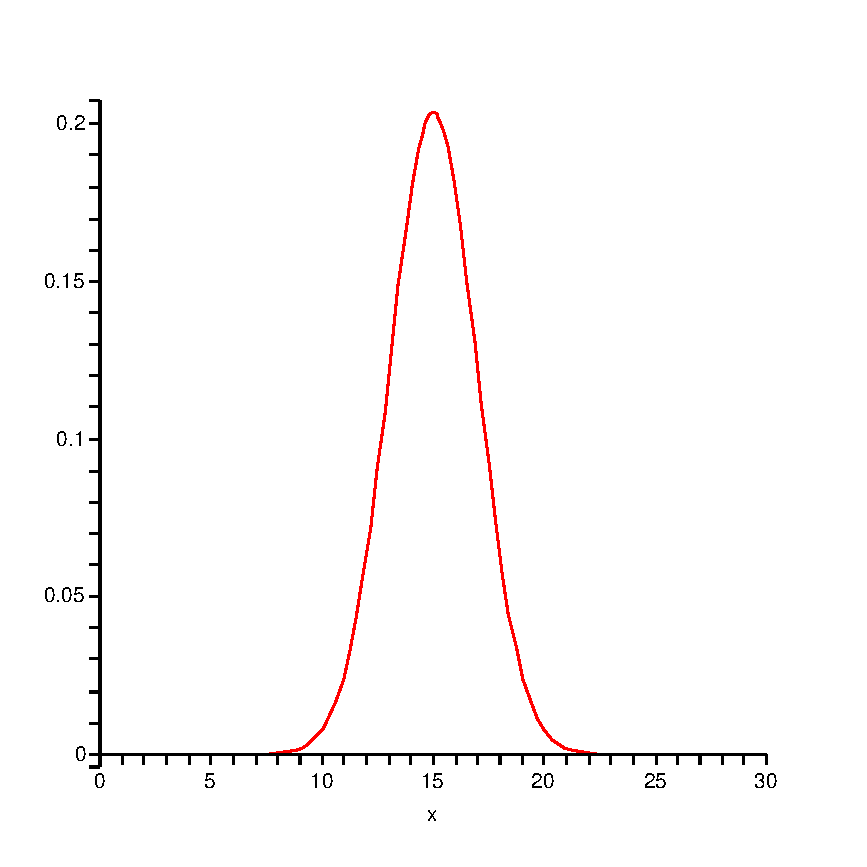
\epsfig{file=pGleichK,scale=0.5}
   \caption{Die Werte der Funktion $P(X=k)$ f�r den Fall $n=30$.}
  \label{fig:pGleichK}
\end{figure}

Weiter gilt 
\\[0.3cm]
\hspace*{1.3cm}
$\displaystyle P(X \leq k) = \frac{\bigl(n!\bigr)^2}{(2\,n)!} \cdot \sum\limits_{l=0}^k {n \choose l}^2$.
\\[0.3cm]
Tragen wir die Werte f�r die Funktion $k \mapsto P(X \leq k)$ in einer Tabelle auf,
so erhalten wir die in Tabelle \ref{tab:pKleinerK} gezeigten Werte.
Wir sehen hier deutlich, dass die vorliegenden Unterschiede zwischen den beiden Kursen mit
hoher Wahrscheinlichkeit auf einen tats�chlich vorhandenen Niveau-Unterschied zur�ck
schlie�en lassen.
\begin{table}[!ht]
  \centering
\framebox{
  \begin{tabular}{|r|l||r|r||r|r|}
\hline
$k$ &          $P(X \leq k)$ & $k$ & $P(X \leq k)$     & $k$ & $P(X \leq k)$ \\
\hline
\hline
  0 & \rule{0pt}{11pt}$8.455616946 \cdot 10^{-18}$ &  10 & $0.0096915941$  &  20 & $0.9979413160$ \\
\hline
  1 & \rule{0pt}{11pt}$7.618510868 \cdot 10^{-15}$ &  11 & $0.0349243550$  &  21 & $0.9996721347$ \\
\hline
  2 & \rule{0pt}{11pt}$1.607632627 \cdot 10^{-12}$ &  12 & $0.0981814847$  &  22 & $0.9999617965$ \\
\hline
  3 & \rule{0pt}{11pt}$1.409866401 \cdot 10^{-10}$ &  13 & $0.2194555084$  &  23 & $0.9999968406$ \\
\hline
  4 & \rule{0pt}{11pt}$6.491442669 \cdot 10^{- 9}$ &  14 & $0.3982728189$  &  24 & $0.9999998218$ \\
\hline
  5 & \rule{0pt}{11pt}$1.782077737 \cdot 10^{- 7}$ &  15 & $0.6017271811$  &  25 & $0.9999999935$ \\
\hline
  6 & \rule{0pt}{11pt}$3.159394076 \cdot 10^{- 6}$ &  16 & $0.7805444916$  &  26 & $0.9999999999$ \\
\hline
  7 & \rule{0pt}{11pt}$3.820354326 \cdot 10^{- 5}$ &  17 & $0.9018185153$  &  27 & $1.0000000000$  \\
\hline
  8 & \rule{0pt}{11pt}$3.278653389 \cdot 10^{- 4}$ &  18 & $0.9650756450$  &  28 & $1.0000000000$  \\
\hline
  9 & \rule{0pt}{11pt}$2.058683970 \cdot 10^{- 3}$ &  19 & $0.9903084059$  &  29 & $1.0000000000$  \\
\hline
  \end{tabular}}
  \caption{Die ersten 60 Werte f�r das Geburtstags-Problem.}
  \label{tab:pKleinerK}
\end{table}
F�r gro�e Werte von $n$ ist die Berechnung der Binomial-Koeffizienten nicht mehr praktikabel.
Dann k�nnen wir in der Formel f�r $P(X=k)$ die Binomial-Koeffizienten durch die Formel von de Moivre ann�hern
und die Fakult�ten $n!$ und $(2\cdot n)!$ k�nnen wir �ber die N�herungsformel von Stirling approximieren-
\begin{enumerate}
\item De Moivre:\quad $\displaystyle
       {n \choose k} \approx \sqrt{\frac{2}{\pi \cdot n}} \cdot 2^n \cdot 
       \exp\left(-\frac{\bigl(k - \frac{1}{2}n\bigr)^2}{\frac{1}{2}n}\right)$.
\item Stirling: \qquad $\displaystyle \;n! \approx \sqrt{2 \cdot \pi \cdot n\;} \cdot 
       \left(\frac{n}{e}\right)^{n}$.
\end{enumerate}
Damit finden wir f�r die Wahrscheinlichkeit $P(X = k)$ die N�herung
\\[0.3cm]
$
\begin{array}[t]{lcl}
P(X = k) 
& = & \displaystyle
      {n \choose k}^2 \cdot \frac{\bigl(n!\bigr)^2}{(2\,n)!}
\\[0.5cm]
& \approx & \displaystyle
\frac{2}{\pi \cdot n} \cdot 4^n \cdot 
       \exp\left(-\frac{\bigl(2 \cdot k - n\bigr)^2}{n}\right) 
       \cdot \frac{2 \cdot \pi \cdot n \cdot 
       \left(\frac{n}{e}\right)^{2\,n}}{
       \sqrt{4 \cdot \pi \cdot n\;} \cdot 
       \left(\frac{2\cdot n}{e}\right)^{2\cdot n}}
\\[0.5cm]
& = & \displaystyle
\frac{2}{\sqrt{\pi \cdot n}} \cdot \exp\left(-\frac{\bigl(2 \cdot k - n\bigr)^2}{n}\right) 
\\[0.5cm]
& \approx & \displaystyle
2 \cdot {2\, n \choose 2\, k} \cdot \left(\frac{1}{2}\right)^{2\,n}
\end{array}
$
\\[0.3cm]
Bei der obigen Ableitung haben wir die N�herungs-Formel von de Moivre im letzten Schritt r�chw�rts angewandt.
Die Wahrscheinlichkeit, die uns eigentlich interessier, ist 
\\[0.3cm]
\hspace*{1.3cm}
$\displaystyle P(X \leq k) = \sum\limits_{l=0}^k P(X=l) \approx 
2 \cdot  \sum\limits_{l=0}^k {2\, n \choose 2\, l} \cdot \left(\frac{1}{2}\right)^{2\,n}
$
\\[0.3cm]
Wir hatten im zweiten Kapitel die Funktion $F^n_p(k)$ wie folgt definiert:
\\[0.3cm]
\hspace*{1.3cm}
$\displaystyle F^n_p(k) := \sum\limits_{l=0}^k {n \choose l} \cdot p^l \cdot (1 - p)^{n-l}$.
\\[0.3cm]
Setzen wir hier f�r $p$ den Wert $\frac{1}{2}$, f�r $n$ den Wert $2\,n$ und f�r $k$ den
Wert $2\,k$ ein, so erhalten wir
\\[0.3cm]
\hspace*{1.3cm}
$\displaystyle 
 F^{2\,n}_{\frac{1}{2}}(2\cdot k) = \sum\limits_{l=0}^{2\,k} {2\,n \choose l} \cdot 
 \left(\frac{1}{2}\right)^{2\,n}$.
\\[0.3cm]
F�r gro�e Werte von $n$ k�nnen wir in dieser Formel die Approximation
\\[0.3cm]
\hspace*{1.3cm}
$\displaystyle {n \choose 2\,l} + {n \choose 2\,l+1} \approx 2 \cdot {n \choose 2\,l}$
\\[0.3cm]
vornehmen, denn die Werte ${n \choose 2\,l}$ und ${n \choose 2\,l+1}$ unterscheiden sich f�r gro�e $n$ und
gro�e $l$ kaum.  F�r kleine Werte von $l$ unterscheiden sich die Werte
 ${n \choose 2\,l}$ und ${n \choose 2\,l+1}$ zwar schon, bei der sp�teren Summation
$\sum\limits_{l=0}^k$ spielen diese Werte aber praktisch keine Rolle.
Damit erhalten wir die N�herungs-Formel
\\[0.3cm]
\hspace*{1.3cm}
$\displaystyle 
 F^{2\,n}_{\frac{1}{2}}(2\cdot k) \approx 2 \cdot
 \sum\limits_{l=0}^k {2\,n \choose 2\,l} \cdot \left(\frac{1}{2}\right)^{2\,n} = P(X \leq k)$.
\\[0.3cm]
Damit haben wir die Wahrscheinlichkeit $P(X \leq k)$ auf die Funktion
$ F^{2\,n}_{\frac{1}{2}}(2\cdot k)$ zur�ck gef�hrt. F�r die Funktion $F^k_p$ hatten wir
aber im zweiten Kapitel die folgende N�herungs-Formel gefunden:
\\[0.3cm]
\hspace*{1.3cm}
$\displaystyle F^n_p(k) \approx \Phi\Biggl(\frac{k- n\,p}{\sqrt{n\,p\,q\,}}\Biggr)$
\\[0.3cm]
Damit haben wir jetzt f�r die Wahrscheinlichkeit $P(X \leq k)$ die N�herungs-Formel 
\\[0.3cm]
\hspace*{1.3cm}
$\displaystyle P(X \leq k) \approx \Phi\Biggl((2\,k- n)\cdot \sqrt{\frac{2}{n}}\Biggr)$
\\[0.3cm]
gefunden.  Dr�cken wir die $\Phi$-Funktion durch die Gau�'sche Fehlerfunktion aus, so
erhalten wir
\\[0.3cm]
\hspace*{1.3cm}
$\displaystyle 
  P(X \leq k) \approx \frac{1}{2} + \frac{1}{2} \cdot \textsl{erf}\biggl(\frac{2\,k- n}{\sqrt{n\;}}\biggr)$.


%%% Local Variables: 
%%% mode: latex
%%% TeX-master: "statistik"
%%% ispell-local-dictionary: "deutsch8"
%%% End: 

%\chapter{Die Ungleichung von Hoeffding}
Angenommen, wir haben eine Urne mit wei�en und schwarzen Kugeln.  Die Wahrscheinlichkeit, dass eine
beliebige Kugel wei� ist, habe den Wert $\mu$, der uns allerdings nicht bekannt ist.  Wir entnehmen
der Urne eine Stichprobe vom Umfang $N$ mit zur�cklegen, so dass die Wahrscheinlichkeit, dass ein
bestimmte Kugel wei� ist, immer den Wert $\mu$ hat.  Ziehen wir bei der Stichprobe insgesamt $k$
wei�e Kugeln, so k�nnen wir die Wahrscheinlichkeit, dass der Bruchteil $k/N$ um mehr als
$\varepsilon$ von der Wahrscheinlichkeit $\mu$ abweicht, durch die
\href{https://en.wikipedia.org/wiki/Hoeffding%27s_inequality}{Hoeffding Ungleichung}
(\href{https://de.wikipedia.org/wiki/Wassily_Hoeffding} Wassily Hoeffding; 1914--1991)
\\[0.2cm]
\hspace*{1.3cm}
$\ds P\biggl(\Bigl|\frac{k}{N} - \mu\Bigr| > \varepsilon\biggr) \leq 2 \cdot\exp\bigl(-2\cdot\varepsilon^2\cdot N\bigr) $
\\[0.2cm] 
absch�tzen.  Diese Formel k�nnen wir nach $N$ umstellen.  Definieren wir $p$ als die
Wahrscheinlichkeit, dass der Anteil der wei�en Kugeln in der Stichprobe um mehr als $\varepsilon$
von der Wahrscheinlichkeit $\mu$ abweicht, setzen wir also
\\[0.2cm]
\hspace*{1.3cm}
$\ds p := P\biggl(\Bigl|\frac{k}{N} - \mu\Bigr| > \varepsilon\biggr)$,
\\[0.2cm]
so haben wir
\\[0.2cm]
\hspace*{1.3cm}
$\ds p \leq 2 \cdot\exp\bigl(-2\cdot\varepsilon^2\cdot N\bigr)$.
\\[0.2cm]
Diese Ungleichung k�nnen wir nach $N$ aufl�sen.  Wir erhalten
\\[0.2cm]
\hspace*{1.3cm}
$\ds N \geq -\frac{\ln(p/2)}{2 \cdot \varepsilon^2}$.
\\[0.2cm]
Nehmen wir beispielsweise an, dass wir einen W�rfel haben und wir sollen die Wahrscheinlichkeit
daf�r, dass eine $6$ gew�rfelt wird, mit einer Genauigkeit von $0.01$ bestimmen.  Die
Wahrscheinlichkeit $p$, dass unser Ergebnis ein Genauigkeit von $0.01$ hat, soll $95\%$ ein.  Dann gilt
\\[0.2cm]
\hspace*{1.3cm}
$p := 0.05$ \quad und \quad $\varepsilon := 0.01$.
\\[0.2cm]
Setzen wir diese Werte in die obige Formel ein, so erhalten wir
\\[0.2cm]
\hspace*{1.3cm}
$N \geq 18444.4$
\\[0.2cm]
und stellen fest, dass wir mindesten $18\,445$ mal w�rfeln m�ssen, um die Wahrscheinlichkeit, dass
eine $6$ gew�rfelt wird mit der erforderlichen Genauigkeit von $0.01$ und $95\%$ Sicherheit bestimmen zu k�nnen.

%%% Local Variables: 
%%% mode: latex
%%% TeX-master: "statistik"
%%% ispell-local-dictionary: "deutsch8"
%%% eval: (setenv "LANG" "de_DE.UTF-8")
%%% End: 


\bibliographystyle{alpha}
\bibliography{cs}

\end{document}

%%% Local Variables: 
%%% mode: latex
%%% TeX-master: t
%%% ispell-local-dictionary: "deutsch8"
%%% End: 
